% ==========================================
% BAB IV IMPLEMENTASI
% ==========================================
\cleardoublepage
\chapter{IMPLEMENTASI}
\label{chap:IV}

Bab ini menerapkan TOGAF Pertahanan Indonesia pada Kemhan RI secara berurutan dari Fase Preliminary hingga Fase Migration Planning.

\section{Fase \textit{Preliminary}}
\label{sec:IV.1}

Fase Preliminary menghasilkan lima keluaran yang menjadi fondasi seluruh fase berikutnya.

\subsection{Prinsip Arsitektur}
\label{sec:IV.1.1}

Prinsip yang digunakan adalah sembilan prinsip arsitektur Pertahanan Indonesia pada Tabel~\ref{tab:III.6}. Untuk memudahkan penerapan, prinsip tersebut dikelompokkan ke dalam enam kategori beserta fase penerapan utamanya, sebagaimana ditunjukkan pada Tabel~\ref{tab:IV.1}.

\begingroup\small\setstretch{1.0}
\begin{longtable}{@{}>{\raggedright\arraybackslash\hspace{0pt}}p{0.187\linewidth}>{\raggedright\arraybackslash\hspace{0pt}}p{0.361\linewidth}>{\raggedright\arraybackslash\hspace{0pt}}p{0.388\linewidth}@{}}
\caption{Pengelompokan Prinsip Arsitektur Pertahanan Indonesia}\label{tab:IV.1}\\
\toprule
\textbf{Kategori} & \textbf{Prinsip} & \textbf{Fase Penerapan Utama}\\
\midrule
\endfirsthead
\multicolumn{3}{@{}l}{\small\itshape \tablename\ \thetable{} (lanjutan)}\\
\toprule
\textbf{Kategori} & \textbf{Prinsip} & \textbf{Fase Penerapan Utama}\\
\midrule
\endhead
\bottomrule
\endlastfoot
Umum & \textit{Smart Defence Oriented}; \textit{Governance \& Compliance} & Seluruh fase\\
Bisnis & \textit{Integrated Command \& Control}; \textit{User-Centric Service} & \textit{Business Architecture}, \textit{Application Architecture}, dan \textit{C6ISR Architecture}\\
Data & \textit{Data as Strategic Asset} & \textit{Data Architecture}\\
Aplikasi & \textit{Interoperability} & \textit{Application Architecture} dan \textit{C6ISR Architecture}\\
Teknologi & \textit{Scalability \& Flexibility}; \textit{Availability \& Reliability} & \textit{Technology Architecture}\\
Keamanan & \textit{Security by Design} & Seluruh fase, terutama \textit{Technology Architecture} dan \textit{C6ISR Architecture}\\
\end{longtable}
\endgroup

Tabel~\ref{tab:IV.1} menunjukkan bahwa setiap domain memiliki prinsip yang mengarahkan perancangannya.

\subsection{Ruang Lingkup}
\label{sec:IV.1.2}

Ruang lingkup arsitektur ditetapkan dalam tiga dimensi, yaitu organisasi yang terlibat, unit organisasi Kemhan RI, dan domain arsitektur, sebagaimana ditunjukkan pada Gambar~\ref{fig:IV.1}.
\begin{figure}[htbp]
\centering
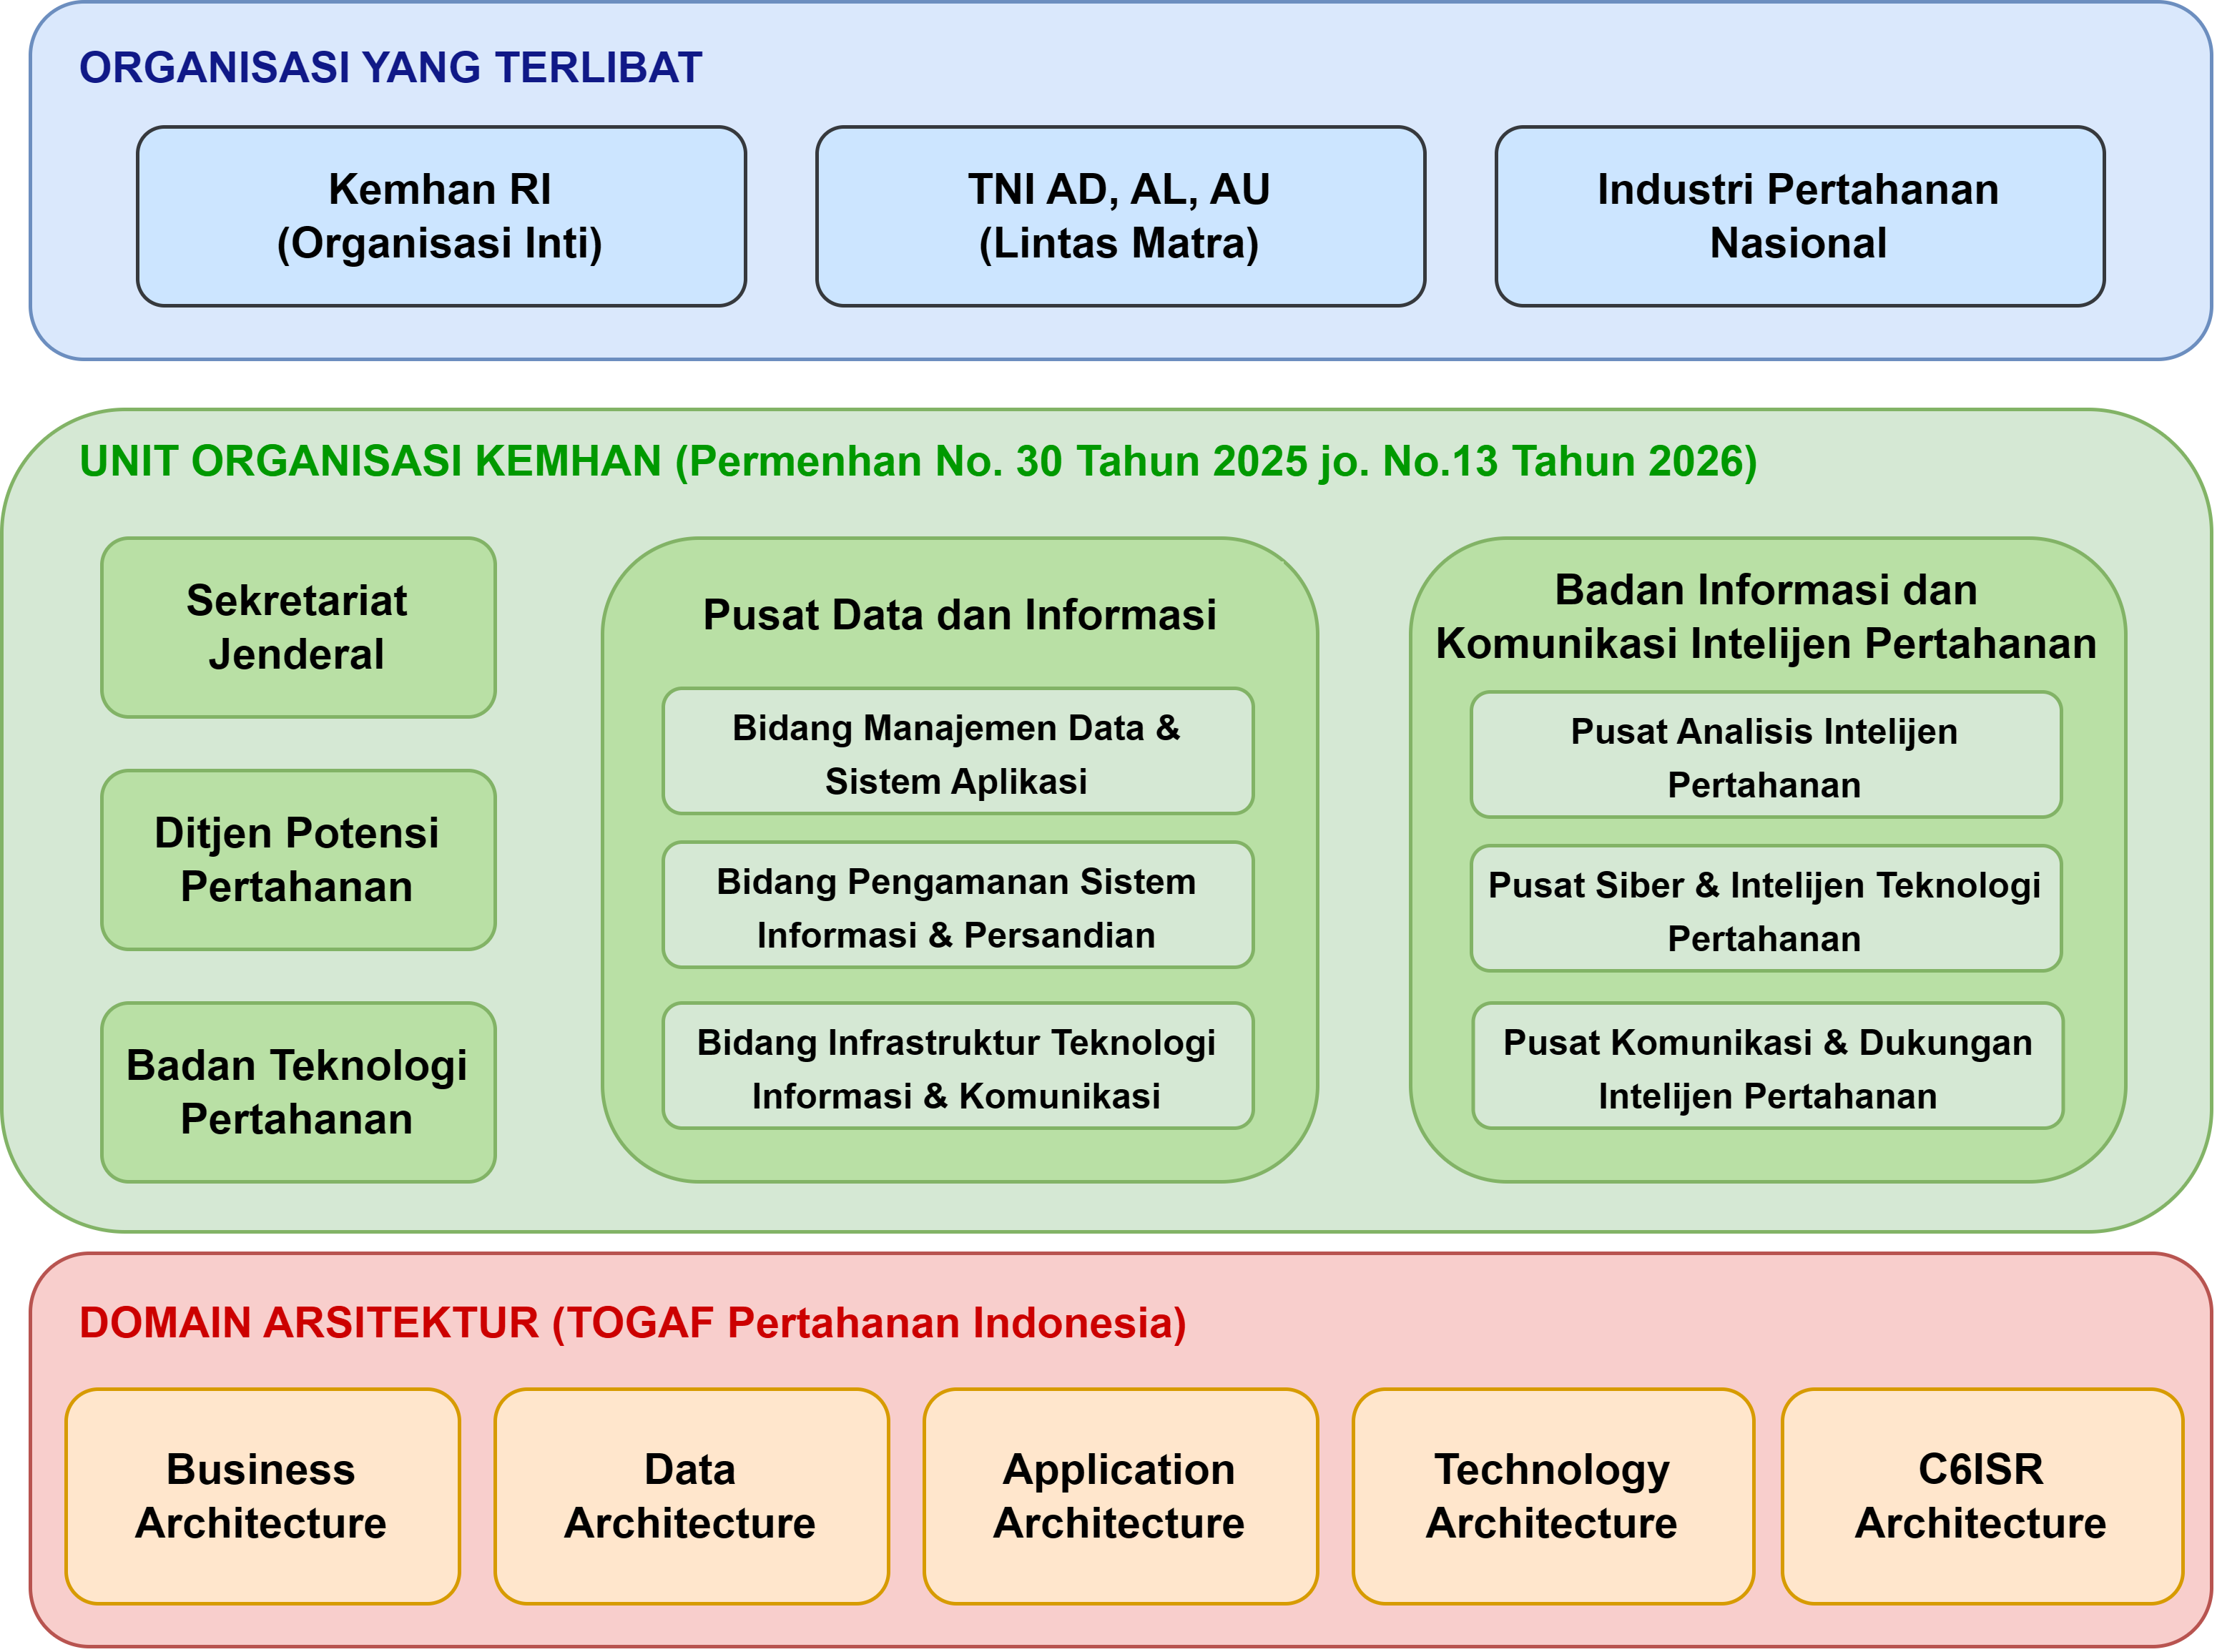
\includegraphics[width=0.99\linewidth,height=0.8\textheight,keepaspectratio]{images/Preliminary - Ruang Lingkup.drawio.png}
\caption{Ruang Lingkup Arsitektur}
\label{fig:IV.1}
\end{figure}

Dari sisi organisasi, Kemhan RI menjadi organisasi inti, ketiga matra TNI terhubung melalui interoperabilitas lintas matra, dan industri pertahanan nasional menjadi mitra ekosistem digital. Dari sisi unit, ruang lingkup mengacu pada Permenhan Nomor 30 Tahun 2025 \cite{Permenhan30Tahun2025} sebagaimana telah diubah dengan Permenhan Nomor 13 Tahun 2026 \cite{Permenhan13Tahun2026}. Pengelolaan data, sistem informasi, dan infrastruktur TIK diselenggarakan oleh Pusat Data dan Informasi yang berkedudukan langsung di bawah Menteri Pertahanan, sedangkan fungsi siber dan intelijen teknologi berada pada Badan Informasi dan Komunikasi Intelijen Pertahanan. Unit lain yang menjadi fokus adalah Sekretariat Jenderal, Ditjen Potensi Pertahanan, dan Badan Teknologi Pertahanan.

Dari sisi domain, pengembangan mencakup lima domain TOGAF Pertahanan Indonesia, yaitu \textit{Business, Data, Application, Technology}, dan \textit{C6ISR Architecture}. Aspek rahasia militer dan operasi tempur tidak dicakup, kecuali pada domain C6ISR yang memodelkan keterhubungan komando dan kendali dengan sistem tempur secara konseptual berdasarkan doktrin, kebijakan, dan sumber terbuka.

\subsection{Identifikasi \textit{Stakeholder}}
\label{sec:IV.1.3}

Identifikasi pemangku kepentingan dilakukan untuk mengenali pihak yang memengaruhi atau dipengaruhi arsitektur beserta \textit{concern}, tingkat pengaruh, dan kebutuhan utamanya. Hasilnya disajikan pada Tabel~\ref{tab:IV.2}.

\begingroup\small\setstretch{1.0}
\begin{longtable}{@{}>{\raggedright\arraybackslash\hspace{0pt}}p{0.063\linewidth}>{\raggedright\arraybackslash\hspace{0pt}}p{0.225\linewidth}>{\raggedright\arraybackslash\hspace{0pt}}p{0.250\linewidth}>{\raggedright\arraybackslash\hspace{0pt}}p{0.125\linewidth}>{\raggedright\arraybackslash\hspace{0pt}}p{0.213\linewidth}@{}}
\caption{Matriks Pemangku Kepentingan}\label{tab:IV.2}\\
\toprule
\textbf{No.} & \textbf{Pemangku Kepentingan} & \textbf{\textit{Concern}} & \textbf{Pengaruh} & \textbf{Kebutuhan Utama}\\
\midrule
\endfirsthead
\multicolumn{5}{@{}l}{\small\itshape \tablename\ \thetable{} (lanjutan)}\\
\toprule
\textbf{No.} & \textbf{Pemangku Kepentingan} & \textbf{\textit{Concern}} & \textbf{Pengaruh} & \textbf{Kebutuhan Utama}\\
\midrule
\endhead
\bottomrule
\endlastfoot
\centering\arraybackslash 1 & Menteri Pertahanan & Arah strategis dan kedaulatan pertahanan & \centering\arraybackslash Sangat tinggi & Informasi eksekutif dan keputusan berbasis data\\
\centering\arraybackslash 2 & Sekretaris Jenderal & Koordinasi dan tata kelola organisasi & \centering\arraybackslash Tinggi & Integrasi lintas unit dan kepatuhan SPBE\\
\centering\arraybackslash 3 & Kepala Pusat Data dan Informasi & Pengelolaan data, sistem informasi, dan infrastruktur TIK & \centering\arraybackslash Sangat tinggi & Infrastruktur TIK terpadu dan tata kelola data\\
\centering\arraybackslash 4 & Pusat Siber dan Intelijen Teknologi Pertahanan & Keamanan dan intelijen siber pertahanan & \centering\arraybackslash Tinggi & Penerapan \textit{security by design} dan pusat operasi keamanan\\
\centering\arraybackslash 5 & Ditjen Potensi Pertahanan & Potensi dan industri pertahanan & \centering\arraybackslash Tinggi & Data potensi dan kolaborasi industri pertahanan\\
\centering\arraybackslash 6 & Ditjen Strategi Pertahanan dan Ditjen Perencanaan Pertahanan & Perumusan strategi dan perencanaan & \centering\arraybackslash Tinggi & Data perencanaan pertahanan yang terintegrasi\\
\centering\arraybackslash 7 & TNI AD, AL, dan AU & Operasi dan interoperabilitas lintas matra & \centering\arraybackslash Tinggi & Pertukaran data dan dukungan komando-kendali\\
\centering\arraybackslash 8 & Badan Teknologi Pertahanan & Pengembangan teknologi pertahanan & \centering\arraybackslash Sedang & Standar teknologi dan dukungan inovasi\\
\centering\arraybackslash 9 & Industri pertahanan nasional & Kolaborasi dan transfer teknologi & \centering\arraybackslash Sedang & Standar terbuka dan interoperabilitas\\
\centering\arraybackslash 10 & Personel dan pengguna layanan & Kemudahan dan keandalan layanan & \centering\arraybackslash Sedang & Layanan digital yang berorientasi pengguna\\
\end{longtable}
\endgroup

Tabel~\ref{tab:IV.2} menunjukkan bahwa Menteri Pertahanan dan Kepala Pusat Data dan Informasi memiliki pengaruh sangat tinggi, sehingga keduanya menjadi sasaran utama rencana komunikasi arsitektur.

\subsection{\textit{Governance}}
\label{sec:IV.1.4}

Permenhan Nomor 30 Tahun 2025 jo. Nomor 13 Tahun 2026 telah menempatkan Pusat Data dan Informasi langsung di bawah Menteri Pertahanan. Namun, mandat unit tersebut bersifat pengelolaan operasional (\textit{run-the-engine}) dan belum mencakup orkestrasi transformasi digital lintas organisasi. Oleh karena itu, tata kelola arsitektur menambahkan fungsi \textit{Chief Digital Transformation Officer} (CDTO) pada tingkat strategis di bawah Menteri Pertahanan. Struktur tata kelola disajikan pada Tabel~\ref{tab:IV.3}.

\begingroup\small\setstretch{1.0}
\begin{longtable}{@{}>{\raggedright\arraybackslash\hspace{0pt}}p{0.065\linewidth}>{\raggedright\arraybackslash\hspace{0pt}}p{0.207\linewidth}>{\raggedright\arraybackslash\hspace{0pt}}p{0.363\linewidth}>{\raggedright\arraybackslash\hspace{0pt}}p{0.272\linewidth}@{}}
\caption{Struktur Tata Kelola Arsitektur}\label{tab:IV.3}\\
\toprule
\textbf{No.} & \textbf{Elemen} & \textbf{Penanggung Jawab} & \textbf{Peran Utama}\\
\midrule
\endfirsthead
\multicolumn{4}{@{}l}{\small\itshape \tablename\ \thetable{} (lanjutan)}\\
\toprule
\textbf{No.} & \textbf{Elemen} & \textbf{Penanggung Jawab} & \textbf{Peran Utama}\\
\midrule
\endhead
\bottomrule
\endlastfoot
\centering\arraybackslash 1 & \textit{Architecture Board} & Diketuai CDTO dengan anggota Kepala Pusat Data dan Informasi, Kepala Badan Informasi dan Komunikasi Intelijen Pertahanan, para Direktur Jenderal terkait, dan perwakilan matra; Sekretaris Jenderal sebagai pengarah & Menetapkan prinsip, menyetujui \textit{Request for Architecture Work}, serta mengesahkan dan meninjau kepatuhan arsitektur\\
\centering\arraybackslash 2 & \textit{Architecture Team} & Dipimpin CDTO, dengan Pusat Data dan Informasi sebagai pelaksana & Menjalankan siklus TOGAF Pertahanan Indonesia pada kelima domain\\
\centering\arraybackslash 3 & Tim Keamanan Siber & Bidang Pengamanan Sistem Informasi dan Persandian bersama Pusat Siber dan Intelijen Teknologi Pertahanan & Menjamin penerapan \textit{security by design} pada seluruh fase\\
\centering\arraybackslash 4 & Pemilik Arsitektur & Menteri Pertahanan sebagai pemilik utama; Kepala Pusat Data dan Informasi sebagai pemilik pelaksana & Memiliki, membiayai, dan menjamin keberlanjutan arsitektur\\
\end{longtable}
\endgroup

Tabel~\ref{tab:IV.3} menunjukkan bahwa CDTO memimpin \textit{Architecture Board} dan \textit{Architecture Team}, sedangkan Pusat Data dan Informasi berperan sebagai pelaksana. Pembagian ini memisahkan fungsi perubahan (\textit{change-the-business}) dari fungsi operasional (\textit{run-the-engine}).

\subsection{Repositori Arsitektur}
\label{sec:IV.1.5}

Repositori arsitektur menyimpan seluruh artefak agar tertata dan dapat ditelusuri antarfase. Repositori dipartisi menurut domain arsitektur, sebagaimana disajikan pada Tabel~\ref{tab:IV.4}.

\begingroup\small\setstretch{1.0}
\begin{longtable}{@{}>{\raggedright\arraybackslash\hspace{0pt}}p{0.311\linewidth}>{\raggedright\arraybackslash\hspace{0pt}}p{0.656\linewidth}@{}}
\caption{Struktur Repositori Arsitektur}\label{tab:IV.4}\\
\toprule
\textbf{Bagian Repositori} & \textbf{Muatan Utama}\\
\midrule
\endfirsthead
\multicolumn{2}{@{}l}{\small\itshape \tablename\ \thetable{} (lanjutan)}\\
\toprule
\textbf{Bagian Repositori} & \textbf{Muatan Utama}\\
\midrule
\endhead
\bottomrule
\endlastfoot
\textit{Business Repository} & Model proses bisnis, peta kapabilitas, \textit{value stream}, dan struktur organisasi\\
\textit{Data Repository} & Model dan kamus data, katalog dan metadata, serta standar Satu Data Pertahanan\\
\textit{Application Repository} & Portofolio dan katalog aplikasi beserta keterkaitannya\\
\textit{Technology Repository} & Standar teknologi, katalog infrastruktur, platform, dan protokol keamanan\\
\textit{C6ISR Repository} & Model arsitektur C6ISR per lapisan, keterhubungan ISR, komando-kendali, dan unsur penindak, serta gambaran situasi bersama (\textit{common operational picture})\\
\textit{Reference Library} & Prinsip arsitektur, katalog regulasi (SPBE dan Satu Data), dan model rujukan TOGAF Pertahanan Indonesia\\
\end{longtable}
\endgroup

Tabel~\ref{tab:IV.4} menunjukkan bahwa \textit{C6ISR Repository} disediakan sebagai bagian tersendiri, sejalan dengan penambahan Fase C6ISR Architecture.

\section{Fase Architecture Vision}
\label{sec:IV.2}

Fase Architecture Vision menetapkan arah arsitektur melalui enam keluaran, yaitu visi dan tujuan, pendorong dan kendala, penilaian kesiapan, risiko dan mitigasi, konsep solusi, serta \textit{Statement of Architecture Work}.

\subsection{Visi, Misi, dan Tujuan Arsitektur}
\label{sec:IV.2.1}

Visi arsitektur transformasi digital Kemhan RI dirumuskan sebagai berikut.

\begin{center}
\fbox{\parbox{0.92\linewidth}{\vspace{4pt}\centering \textit{“Terwujudnya arsitektur transformasi digital pertahanan yang terintegrasi, aman, dan berorientasi pertahanan cerdas untuk mewujudkan keunggulan informasi serta mendukung pengambilan keputusan yang cepat dan tepat di lingkungan Kemhan RI dan TNI.”}\vspace{4pt}}}
\end{center}

Visi tersebut dijabarkan ke dalam lima misi berikut.
\begin{enumerate}[label=\arabic*.]
\item Mewujudkan interoperabilitas dan integrasi data lintas unit Kemhan RI dan ketiga matra.
\item Menerapkan keamanan siber sejak perancangan pada seluruh sistem pertahanan.
\item Menyediakan layanan digital yang andal dan berorientasi pengguna.
\item Membangun fondasi kapabilitas C6ISR untuk mendukung komando dan kendali terintegrasi.
\item Menyelenggarakan tata kelola digital yang selaras dengan SPBE dan Satu Data Indonesia.
\end{enumerate}

Visi dan misi tersebut diturunkan menjadi tujuan strategis yang masing-masing tertaut pada prinsip arsitektur, sebagaimana disajikan pada Tabel~\ref{tab:IV.5}.

\begingroup\small\setstretch{1.0}
\begin{longtable}{@{}>{\raggedright\arraybackslash\hspace{0pt}}p{0.067\linewidth}>{\raggedright\arraybackslash\hspace{0pt}}p{0.549\linewidth}>{\raggedright\arraybackslash\hspace{0pt}}p{0.321\linewidth}@{}}
\caption{Tujuan Strategis Arsitektur dan Prinsip Terkait}\label{tab:IV.5}\\
\toprule
\textbf{No.} & \textbf{Tujuan Strategis} & \textbf{Prinsip Terkait}\\
\midrule
\endfirsthead
\multicolumn{3}{@{}l}{\small\itshape \tablename\ \thetable{} (lanjutan)}\\
\toprule
\textbf{No.} & \textbf{Tujuan Strategis} & \textbf{Prinsip Terkait}\\
\midrule
\endhead
\bottomrule
\endlastfoot
\centering\arraybackslash 1 & Mewujudkan integrasi data dan sistem antara Kemhan RI dan matra & \textit{Interoperability}\\
\centering\arraybackslash 2 & Memperkuat keamanan siber pertahanan secara menyeluruh & \textit{Security by Design}\\
\centering\arraybackslash 3 & Mengelola data pertahanan sebagai aset strategis pengambilan keputusan & \textit{Data as Strategic Asset}\\
\centering\arraybackslash 4 & Menyiapkan kapabilitas C6ISR dan komando-kendali terintegrasi & \textit{Integrated Command \& Control}\\
\centering\arraybackslash 5 & Meningkatkan kualitas layanan dan efektivitas personel & \textit{User-Centric Service}\\
\centering\arraybackslash 6 & Menjamin kepatuhan tata kelola digital pertahanan & \textit{Governance \& Compliance}\\
\end{longtable}
\endgroup

\subsection{Pendorong dan Kendala}
\label{sec:IV.2.2}

Pendorong dan kendala transformasi dirangkum pada Tabel~\ref{tab:IV.6}. Pendorong utama berasal dari arah RPJPN 2025–2045 \cite{UU59Tahun2024} serta kebijakan SPBE \cite{Perpres95Tahun2018} dan percepatan transformasi digital \cite{Perpres82Tahun2023}.

\begingroup\small\setstretch{1.0}
\begin{longtable}{@{}>{\raggedright\arraybackslash\hspace{0pt}}p{0.235\linewidth}>{\raggedright\arraybackslash\hspace{0pt}}p{0.732\linewidth}@{}}
\caption{Pendorong dan Kendala Transformasi Digital Pertahanan}\label{tab:IV.6}\\
\toprule
\textbf{Aspek} & \textbf{Uraian}\\
\midrule
\endfirsthead
\multicolumn{2}{@{}l}{\small\itshape \tablename\ \thetable{} (lanjutan)}\\
\toprule
\textbf{Aspek} & \textbf{Uraian}\\
\midrule
\endhead
\bottomrule
\endlastfoot
Pendorong & Arah modernisasi pertahanan dalam RPJPN 2025–2045; kebijakan SPBE dan Satu Data Indonesia; meningkatnya ancaman siber dan tuntutan operasi multidomain; kebutuhan interoperabilitas lintas matra; serta tuntutan pengambilan keputusan berbasis data.\\
Kendala & Fragmentasi sistem dan data yang tersilo; keterbatasan SDM digital; keberadaan sistem lama (\textit{legacy}); aspek kerahasiaan pertahanan; serta keterbatasan anggaran dan waktu.\\
\end{longtable}
\endgroup

\subsection{Penilaian Kapabilitas dan Kesiapan}
\label{sec:IV.2.3}

Penilaian kesiapan mengukur kemampuan organisasi menjalankan perubahan menuju arsitektur target. Penilaian didasarkan pada kondisi yang diuraikan pada Subbab~\ref{sec:I.1}, termasuk empat permasalahan prioritas Satu Data Pertahanan, yaitu kelembagaan dan koordinasi, kualitas data, integrasi sistem, dan kapasitas SDM \cite{Pusdatin2026SatuData}. Hasilnya disajikan pada Tabel~\ref{tab:IV.7}.

\begingroup\small\setstretch{1.0}
\begin{longtable}{@{}>{\raggedright\arraybackslash\hspace{0pt}}p{0.065\linewidth}>{\raggedright\arraybackslash\hspace{0pt}}p{0.240\linewidth}>{\raggedright\arraybackslash\hspace{0pt}}p{0.427\linewidth}>{\raggedright\arraybackslash\hspace{0pt}}p{0.175\linewidth}@{}}
\caption{Penilaian Kesiapan Transformasi}\label{tab:IV.7}\\
\toprule
\textbf{No.} & \textbf{Faktor} & \textbf{Kondisi Saat Ini} & \textbf{Tingkat Kesiapan}\\
\midrule
\endfirsthead
\multicolumn{4}{@{}l}{\small\itshape \tablename\ \thetable{} (lanjutan)}\\
\toprule
\textbf{No.} & \textbf{Faktor} & \textbf{Kondisi Saat Ini} & \textbf{Tingkat Kesiapan}\\
\midrule
\endhead
\bottomrule
\endlastfoot
\centering\arraybackslash 1 & Kepemimpinan dan tata kelola & Pusat Data dan Informasi telah berdiri langsung di bawah Menteri, tetapi mandat orkestrasi transformasi belum ada & \centering\arraybackslash Sedang\\
\centering\arraybackslash 2 & SDM digital & Kompetensi digital masih terbatas dan tersebar antarunit & \centering\arraybackslash Rendah–Sedang\\
\centering\arraybackslash 3 & Data dan interoperabilitas & Data masih tersilo dan standar antarunit belum seragam & \centering\arraybackslash Rendah\\
\centering\arraybackslash 4 & Infrastruktur teknologi & Infrastruktur tersedia, tetapi belum sepenuhnya terpadu & \centering\arraybackslash Sedang\\
\centering\arraybackslash 5 & Keamanan siber & Fungsi keamanan siber tersedia pada Pusat Data dan Informasi serta Pusat Siber dan Intelijen Teknologi Pertahanan & \centering\arraybackslash Sedang\\
\centering\arraybackslash 6 & Regulasi dan kebijakan & Didukung kebijakan SPBE, Satu Data, dan RPJPN 2025–2045 & \centering\arraybackslash Tinggi\\
\end{longtable}
\endgroup

Tabel~\ref{tab:IV.7} menunjukkan bahwa kesiapan terendah terdapat pada data dan interoperabilitas serta SDM digital, sedangkan kesiapan tertinggi terdapat pada dukungan regulasi. Dengan demikian, hambatan utama transformasi terletak pada tata kelola data dan kapasitas organisasi.

\subsection{Risiko dan Mitigasi}
\label{sec:IV.2.4}

Risiko transformasi diidentifikasi untuk mengantisipasi hambatan yang dapat menggagalkan pencapaian arsitektur target. Setiap risiko disertai tindakan mitigasi, sebagaimana disajikan pada Tabel~\ref{tab:IV.8}.

\begingroup\small\setstretch{1.0}
\begin{longtable}{@{}>{\raggedright\arraybackslash\hspace{0pt}}p{0.065\linewidth}>{\raggedright\arraybackslash\hspace{0pt}}p{0.272\linewidth}>{\raggedright\arraybackslash\hspace{0pt}}p{0.246\linewidth}>{\raggedright\arraybackslash\hspace{0pt}}p{0.324\linewidth}@{}}
\caption{Risiko Transformasi dan Mitigasi}\label{tab:IV.8}\\
\toprule
\textbf{No.} & \textbf{Risiko} & \textbf{Dampak} & \textbf{Mitigasi}\\
\midrule
\endfirsthead
\multicolumn{4}{@{}l}{\small\itshape \tablename\ \thetable{} (lanjutan)}\\
\toprule
\textbf{No.} & \textbf{Risiko} & \textbf{Dampak} & \textbf{Mitigasi}\\
\midrule
\endhead
\bottomrule
\endlastfoot
\centering\arraybackslash 1 & Resistensi perubahan organisasi & Adopsi arsitektur berjalan lambat & Manajemen perubahan, dukungan pimpinan, dan fungsi CDTO\\
\centering\arraybackslash 2 & Keterbatasan SDM digital & Kualitas implementasi menurun & Pelatihan, rekrutmen, dan kerja sama kelembagaan\\
\centering\arraybackslash 3 & Kompleksitas integrasi sistem \textit{legacy} & Keterlambatan dan pembengkakan biaya & Bertahapan, penggunaan \textit{middleware}/API, dan standar terbuka\\
\centering\arraybackslash 4 & Ancaman siber selama transisi & Kebocoran atau gangguan data & Penerapan \textit{security by design} dan penguatan fungsi keamanan siber\\
\centering\arraybackslash 5 & Ketergantungan pada teknologi asing & Risiko terhadap kedaulatan data & Mengutamakan teknologi dalam negeri dan standar terbuka\\
\centering\arraybackslash 6 & Keterbatasan anggaran dan waktu & Cakupan target tidak tercapai & Prioritas berbasis nilai dan peta jalan bertahap\\
\end{longtable}
\endgroup

\subsection{Konsep Solusi}
\label{sec:IV.2.5}

Konsep solusi memberikan gambaran menyeluruh mengenai arsitektur target. Konsep ini disusun berlapis, mulai dari infrastruktur terpadu sebagai fondasi, platform interoperabilitas dan Satu Data Pertahanan sebagai simpul integrasi, kapabilitas C6ISR sebagai inti operasional, hingga layanan digital bagi seluruh pemangku kepentingan, sebagaimana ditunjukkan pada Gambar~\ref{fig:IV.2}.
\begin{figure}[htbp]
\centering
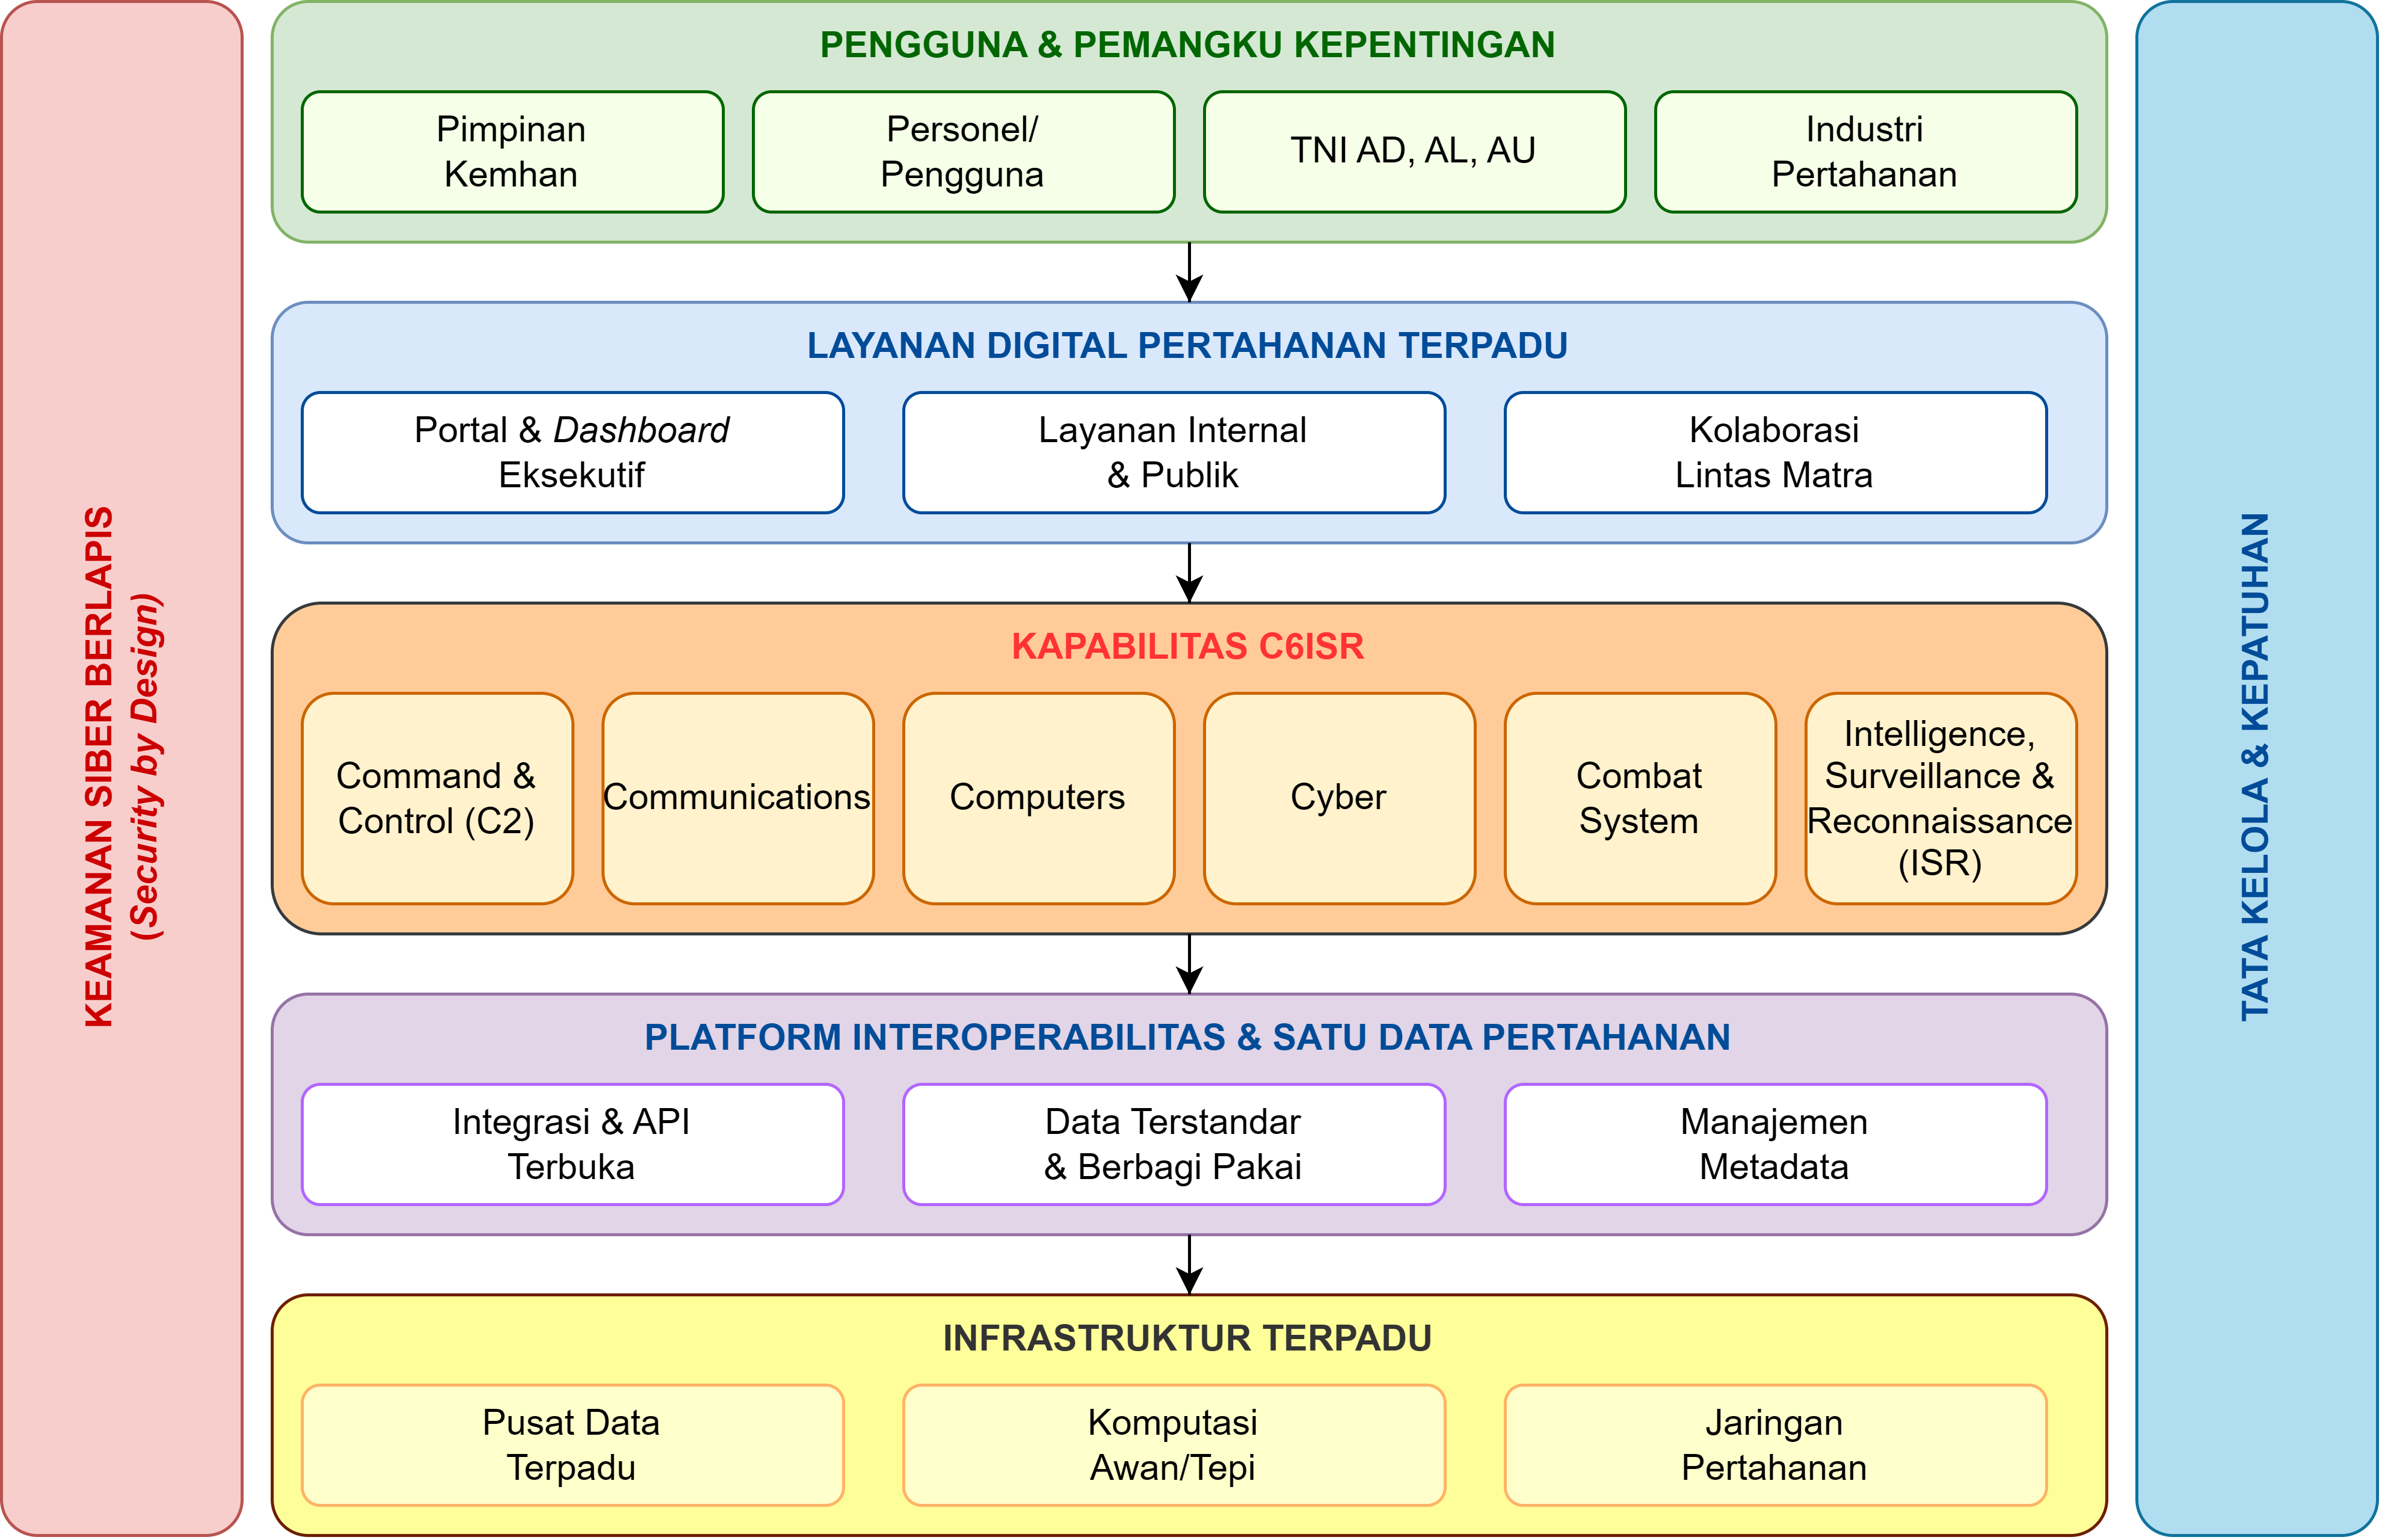
\includegraphics[width=0.99\linewidth,height=0.8\textheight,keepaspectratio]{images/Solusi Arsitektur Target.drawio.png}
\caption{Konsep Solusi Arsitektur Target}
\label{fig:IV.2}
\end{figure}

Gambar~\ref{fig:IV.2} menunjukkan bahwa keamanan siber berlapis serta tata kelola dan kepatuhan membentang pada seluruh lapisan. Hal ini sejalan dengan prinsip \textit{Security by Design} dan \textit{Governance \& Compliance} yang berlaku pada seluruh fase.

\subsection{\textit{Statement of Architecture Work}}
\label{sec:IV.2.6}

\textit{Statement of Architecture Work} (SoAW) merupakan dokumen kesepakatan kerja yang menetapkan ruang lingkup, tujuan, keluaran, pelaksana, dan batasan pekerjaan arsitektur. Ringkasan SoAW disajikan pada Tabel~\ref{tab:IV.9}.

\begingroup\small\setstretch{1.0}
\begin{longtable}{@{}>{\raggedright\arraybackslash\hspace{0pt}}p{0.235\linewidth}>{\raggedright\arraybackslash\hspace{0pt}}p{0.732\linewidth}@{}}
\caption{Ringkasan \textit{Statement of Architecture Work}}\label{tab:IV.9}\\
\toprule
\textbf{Komponen} & \textbf{Uraian}\\
\midrule
\endfirsthead
\multicolumn{2}{@{}l}{\small\itshape \tablename\ \thetable{} (lanjutan)}\\
\toprule
\textbf{Komponen} & \textbf{Uraian}\\
\midrule
\endhead
\bottomrule
\endlastfoot
Nama pekerjaan & Perancangan arsitektur transformasi digital Kemhan RI berbasis TOGAF Pertahanan Indonesia\\
Ruang lingkup & Kemhan RI, ketiga matra, dan industri pertahanan pada lima domain arsitektur\\
Tujuan & Mewujudkan arsitektur yang terintegrasi, aman, dan berorientasi pertahanan cerdas sesuai visi dan tujuan strategis\\
Keluaran & Arsitektur \textit{baseline} dan target setiap domain, paket pekerjaan, roadmap, serta rencana migrasi 2026–2030\\
Pelaksana & \textit{Architecture Board}, \textit{Architecture Team}, dan Tim Keamanan Siber\\
Prinsip dan batasan & Sembilan prinsip arsitektur serta kepatuhan terhadap SPBE, Satu Data, dan regulasi pertahanan\\
Jadwal & Bertahap mengikuti siklus TOGAF Pertahanan Indonesia dari Fase Preliminary hingga Fase Migration Planning\\
\end{longtable}
\endgroup

\section{Fase Business Architecture}
\label{sec:IV.3}

Fase Business Architecture menjabarkan visi arsitektur menjadi struktur organisasi, \textit{value stream}, dan kapabilitas pertahanan sesuai Tabel~\ref{tab:III.9}. Struktur organisasi mengacu pada Permenhan Nomor 30 Tahun 2025 \cite{Permenhan30Tahun2025} sebagaimana telah diubah dengan Permenhan Nomor 13 Tahun 2026 \cite{Permenhan13Tahun2026}.

\subsection{Struktur Organisasi dan Tata Kelola}
\label{sec:IV.3.1}

Struktur organisasi Kemhan RI pada kondisi \textit{baseline} menjadi dasar untuk mengidentifikasi fungsi yang telah ada maupun fungsi yang belum memiliki penanggung jawab. Struktur tersebut disajikan pada Gambar~\ref{fig:IV.3}.
\begin{figure}[htbp]
\centering
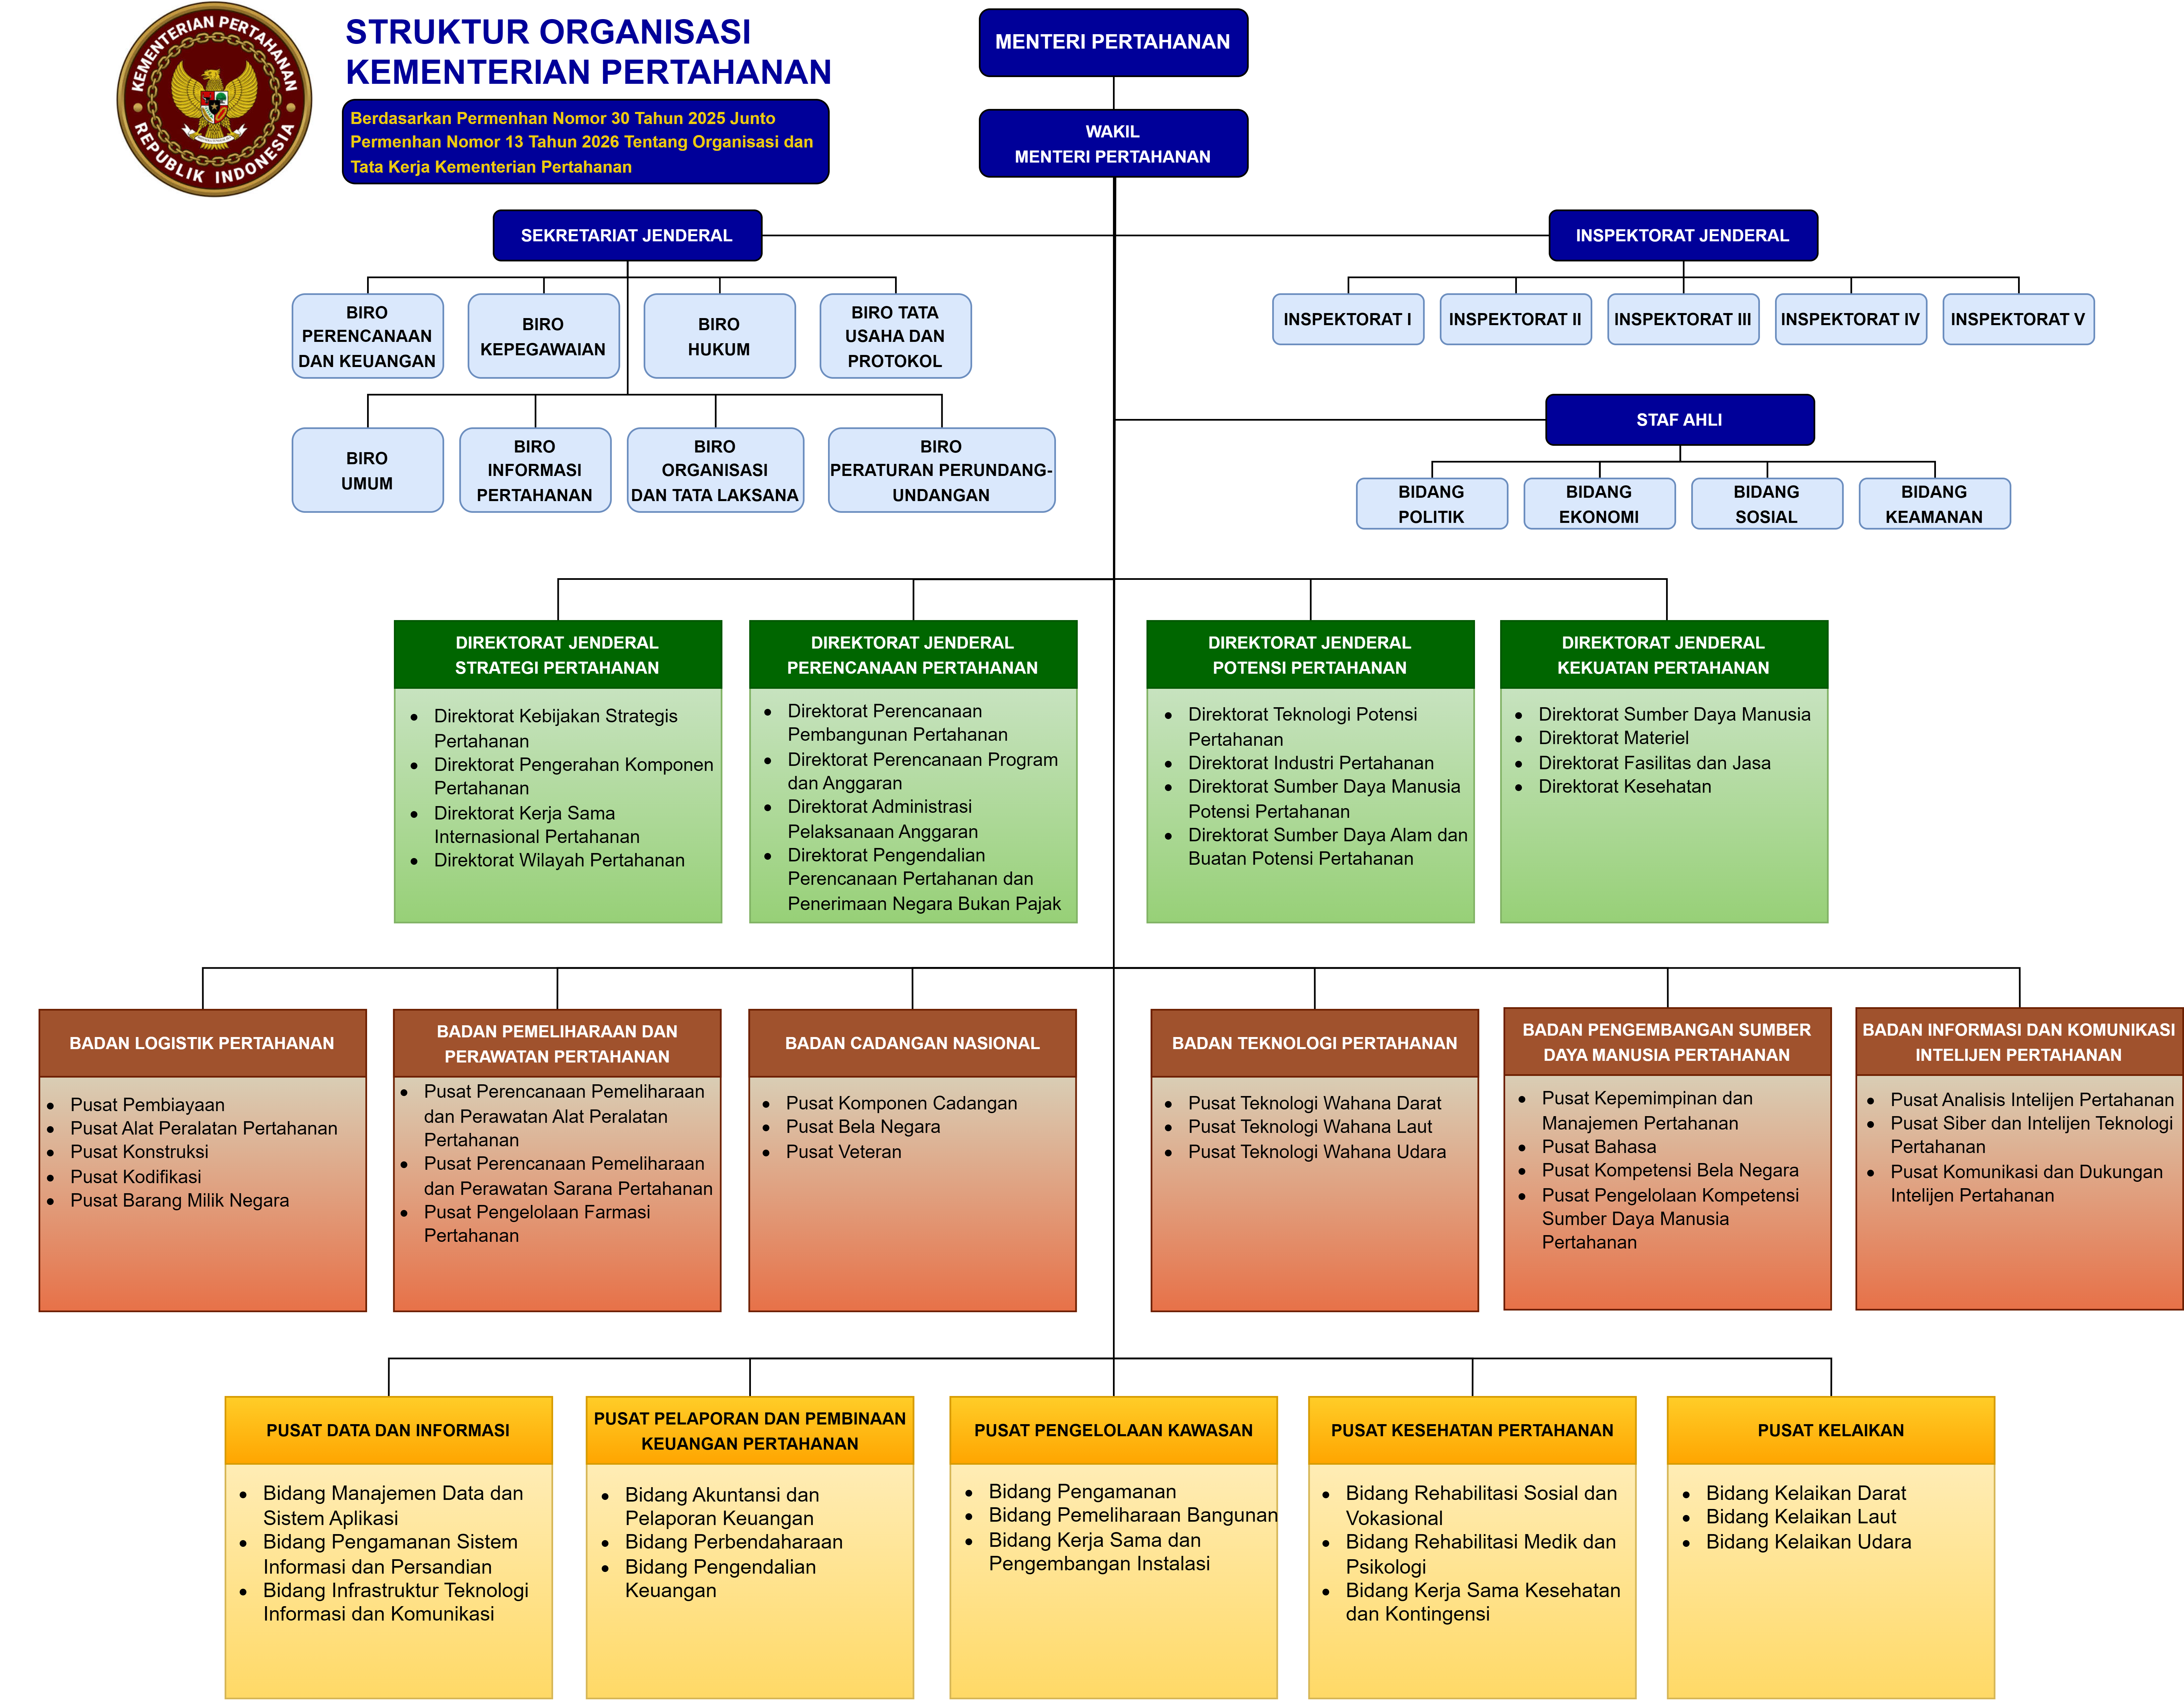
\includegraphics[width=0.99\linewidth,height=0.8\textheight,keepaspectratio]{images/Struktur Organisasi Kemhan Permenhan 30_2025 dan 13_2026.drawio.png}
\caption{Struktur Organisasi dan Tata Kerja Kemhan RI}
\label{fig:IV.3}
\end{figure}

Gambar~\ref{fig:IV.3} menunjukkan bahwa Kemhan RI dipimpin oleh Menteri Pertahanan yang dibantu Wakil Menteri Pertahanan. Unsur di bawahnya terdiri atas Sekretariat Jenderal, Inspektorat Jenderal, Staf Ahli, 4 direktorat jenderal, 6 badan, dan 5 pusat. Fungsi utama setiap unit dirangkum pada Tabel~\ref{tab:IV.10}.

\begingroup\small\setstretch{1.0}
\begin{longtable}{@{}>{\raggedright\arraybackslash\hspace{0pt}}p{0.067\linewidth}>{\raggedright\arraybackslash\hspace{0pt}}p{0.321\linewidth}>{\raggedright\arraybackslash\hspace{0pt}}p{0.549\linewidth}@{}}
\caption{Fungsi Utama Unit Organisasi Kemhan RI}\label{tab:IV.10}\\
\toprule
\textbf{No.} & \textbf{Unit Organisasi} & \textbf{Fungsi Utama}\\
\midrule
\endfirsthead
\multicolumn{3}{@{}l}{\small\itshape \tablename\ \thetable{} (lanjutan)}\\
\toprule
\textbf{No.} & \textbf{Unit Organisasi} & \textbf{Fungsi Utama}\\
\midrule
\endhead
\bottomrule
\endlastfoot
\centering\arraybackslash 1 & Inspektorat Jenderal & Pengawasan intern di lingkungan Kemhan\\
\centering\arraybackslash 2 & Sekretariat Jenderal & Koordinasi pelaksanaan tugas, pembinaan, dan dukungan administrasi seluruh unsur Kemhan\\
\centering\arraybackslash 3 & Staf Ahli & Rekomendasi atas isu strategis kepada Menteri sesuai bidangnya\\
\centering\arraybackslash 4 & Ditjen Strategi Pertahanan & Kebijakan di bidang strategi pertahanan\\
\centering\arraybackslash 5 & Ditjen Perencanaan Pertahanan & Kebijakan di bidang perencanaan pertahanan\\
\centering\arraybackslash 6 & Ditjen Potensi Pertahanan & Kebijakan di bidang potensi pertahanan, termasuk pembinaan industri pertahanan\\
\centering\arraybackslash 7 & Ditjen Kekuatan Pertahanan & Kebijakan di bidang kekuatan pertahanan\\
\centering\arraybackslash 8 & Badan Logistik Pertahanan & Pengelolaan logistik dan sarana pertahanan\\
\centering\arraybackslash 9 & Badan Pemeliharaan dan Perawatan Pertahanan & Pemeliharaan Alpalhankam dan sarana pertahanan serta koordinasi farmasi pertahanan\\
\centering\arraybackslash 10 & Badan Cadangan Nasional & Pembinaan komponen cadangan, bela negara, dan keveteranan\\
\centering\arraybackslash 11 & Badan Teknologi Pertahanan & Pengembangan teknologi wahana darat, laut, dan udara\\
\centering\arraybackslash 12 & Badan Pengembangan Sumber Daya Manusia Pertahanan & Pengembangan sumber daya manusia pertahanan\\
\centering\arraybackslash 13 & Badan Informasi dan Komunikasi Intelijen Pertahanan & Analisis intelijen, siber dan intelijen teknologi, serta komunikasi dan dukungan intelijen pertahanan\\
\centering\arraybackslash 14 & Pusat Data dan Informasi & Sistem informasi, infrastruktur TIK, pengamanan sistem informasi dan persandian, serta manajemen Satu Data Pertahanan\\
\centering\arraybackslash 15 & Pusat Pelaporan dan Pembinaan Keuangan Pertahanan & Pelaporan dan pembinaan pengelolaan keuangan pertahanan\\
\centering\arraybackslash 16 & Pusat Pengelolaan Kawasan & Pengamanan, pemeliharaan bangunan, serta kerja sama dan pengembangan instalasi Kawasan IPSC\\
\centering\arraybackslash 17 & Pusat Kesehatan Pertahanan & Rehabilitasi pascacedera, penyandang disabilitas, dan kesehatan pertahanan\\
\centering\arraybackslash 18 & Pusat Kelaikan & Sertifikasi kelaikan Alpalhankam, konstruksi, satwa, dan fasilitas pertahanan\\
\end{longtable}
\endgroup

Tabel~\ref{tab:IV.10} menunjukkan bahwa fungsi data, sistem informasi, dan infrastruktur TIK berada pada Pusat Data dan Informasi, sedangkan fungsi siber dan intelijen teknologi berada pada Badan Informasi dan Komunikasi Intelijen Pertahanan. Dari sisi tata kelola, keputusan berjalan berjenjang dari Menteri Pertahanan ke unit eselon I dengan Sekretariat Jenderal sebagai koordinator lintas unit. Pada aspek komando, Kemhan RI berperan pada kebijakan, standar, dan sumber daya pertahanan, sedangkan komando penggunaan kekuatan berada pada Mabes TNI.

Meskipun demikian, pengelolaan teknologi informasi dan data masih bersifat operasional pada masing-masing unit. Akibatnya, sistem berjalan terfragmentasi dan data tersilo antarunit. Kondisi ini menunjukkan bahwa struktur saat ini belum memiliki unit yang memegang mandat transformasi digital lintas organisasi.

\subsection{\textit{Value Stream}}
\label{sec:IV.3.2}

\textit{Value stream} menggambarkan penyelenggaraan pertahanan sebagai aliran nilai horizontal lintas unit. Dengan cara ini, kapabilitas dapat diidentifikasi tanpa terikat sekat organisasi. \textit{Value stream} Kemhan RI disajikan pada Gambar~\ref{fig:IV.4}.
\begin{figure}[htbp]
\centering
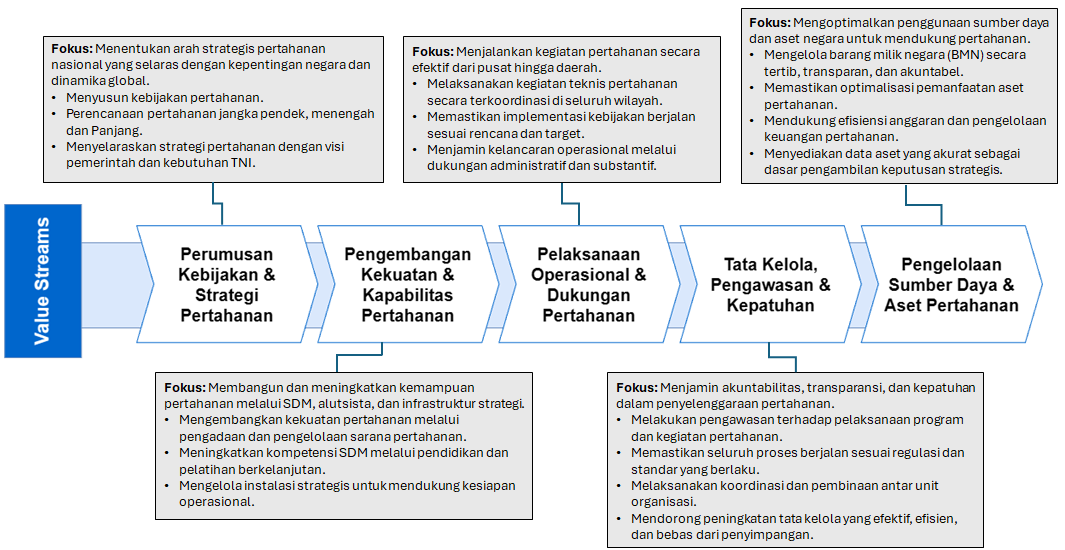
\includegraphics[width=0.99\linewidth,height=0.8\textheight,keepaspectratio]{images/Value Stream Kemhan dan Penjelasan.png}
\caption{\textit{Value Stream} Kemhan RI}
\label{fig:IV.4}
\end{figure}

Gambar~\ref{fig:IV.4} menunjukkan lima aliran nilai yang berurutan, yaitu:
\begin{enumerate}[label=\arabic*.]
\item Perumusan Kebijakan dan Strategi Pertahanan, yang menetapkan arah strategis serta perencanaan pertahanan jangka pendek, menengah, dan panjang;
\item Pengembangan Kekuatan dan Kapabilitas Pertahanan, yang membangun kemampuan melalui SDM, alutsista, dan infrastruktur strategis;
\item Pelaksanaan Operasional dan Dukungan Pertahanan, yang menjalankan kegiatan pertahanan secara terkoordinasi dari pusat hingga daerah;
\item Tata Kelola, Pengawasan, dan Kepatuhan, yang menjamin akuntabilitas, transparansi, dan kepatuhan terhadap regulasi; serta
\item Pengelolaan Sumber Daya dan Aset Pertahanan, yang mengoptimalkan barang milik negara, aset, dan keuangan pertahanan.
\end{enumerate}

Kelima aliran nilai tersebut menjadi dasar penurunan peta kapabilitas.

\subsection{Peta Kapabilitas}
\label{sec:IV.3.3}

Peta kapabilitas (\textit{business capability map}) menjabarkan kemampuan yang diperlukan untuk menjalankan kelima aliran nilai. Pendekatan berbasis kapabilitas memisahkan “apa yang dilakukan” dari “siapa yang melakukannya”, sehingga arsitektur tetap stabil meskipun organisasi ditata ulang. Peta kapabilitas Kemhan RI disajikan pada Gambar~\ref{fig:IV.5}.
\begin{figure}[htbp]
\centering
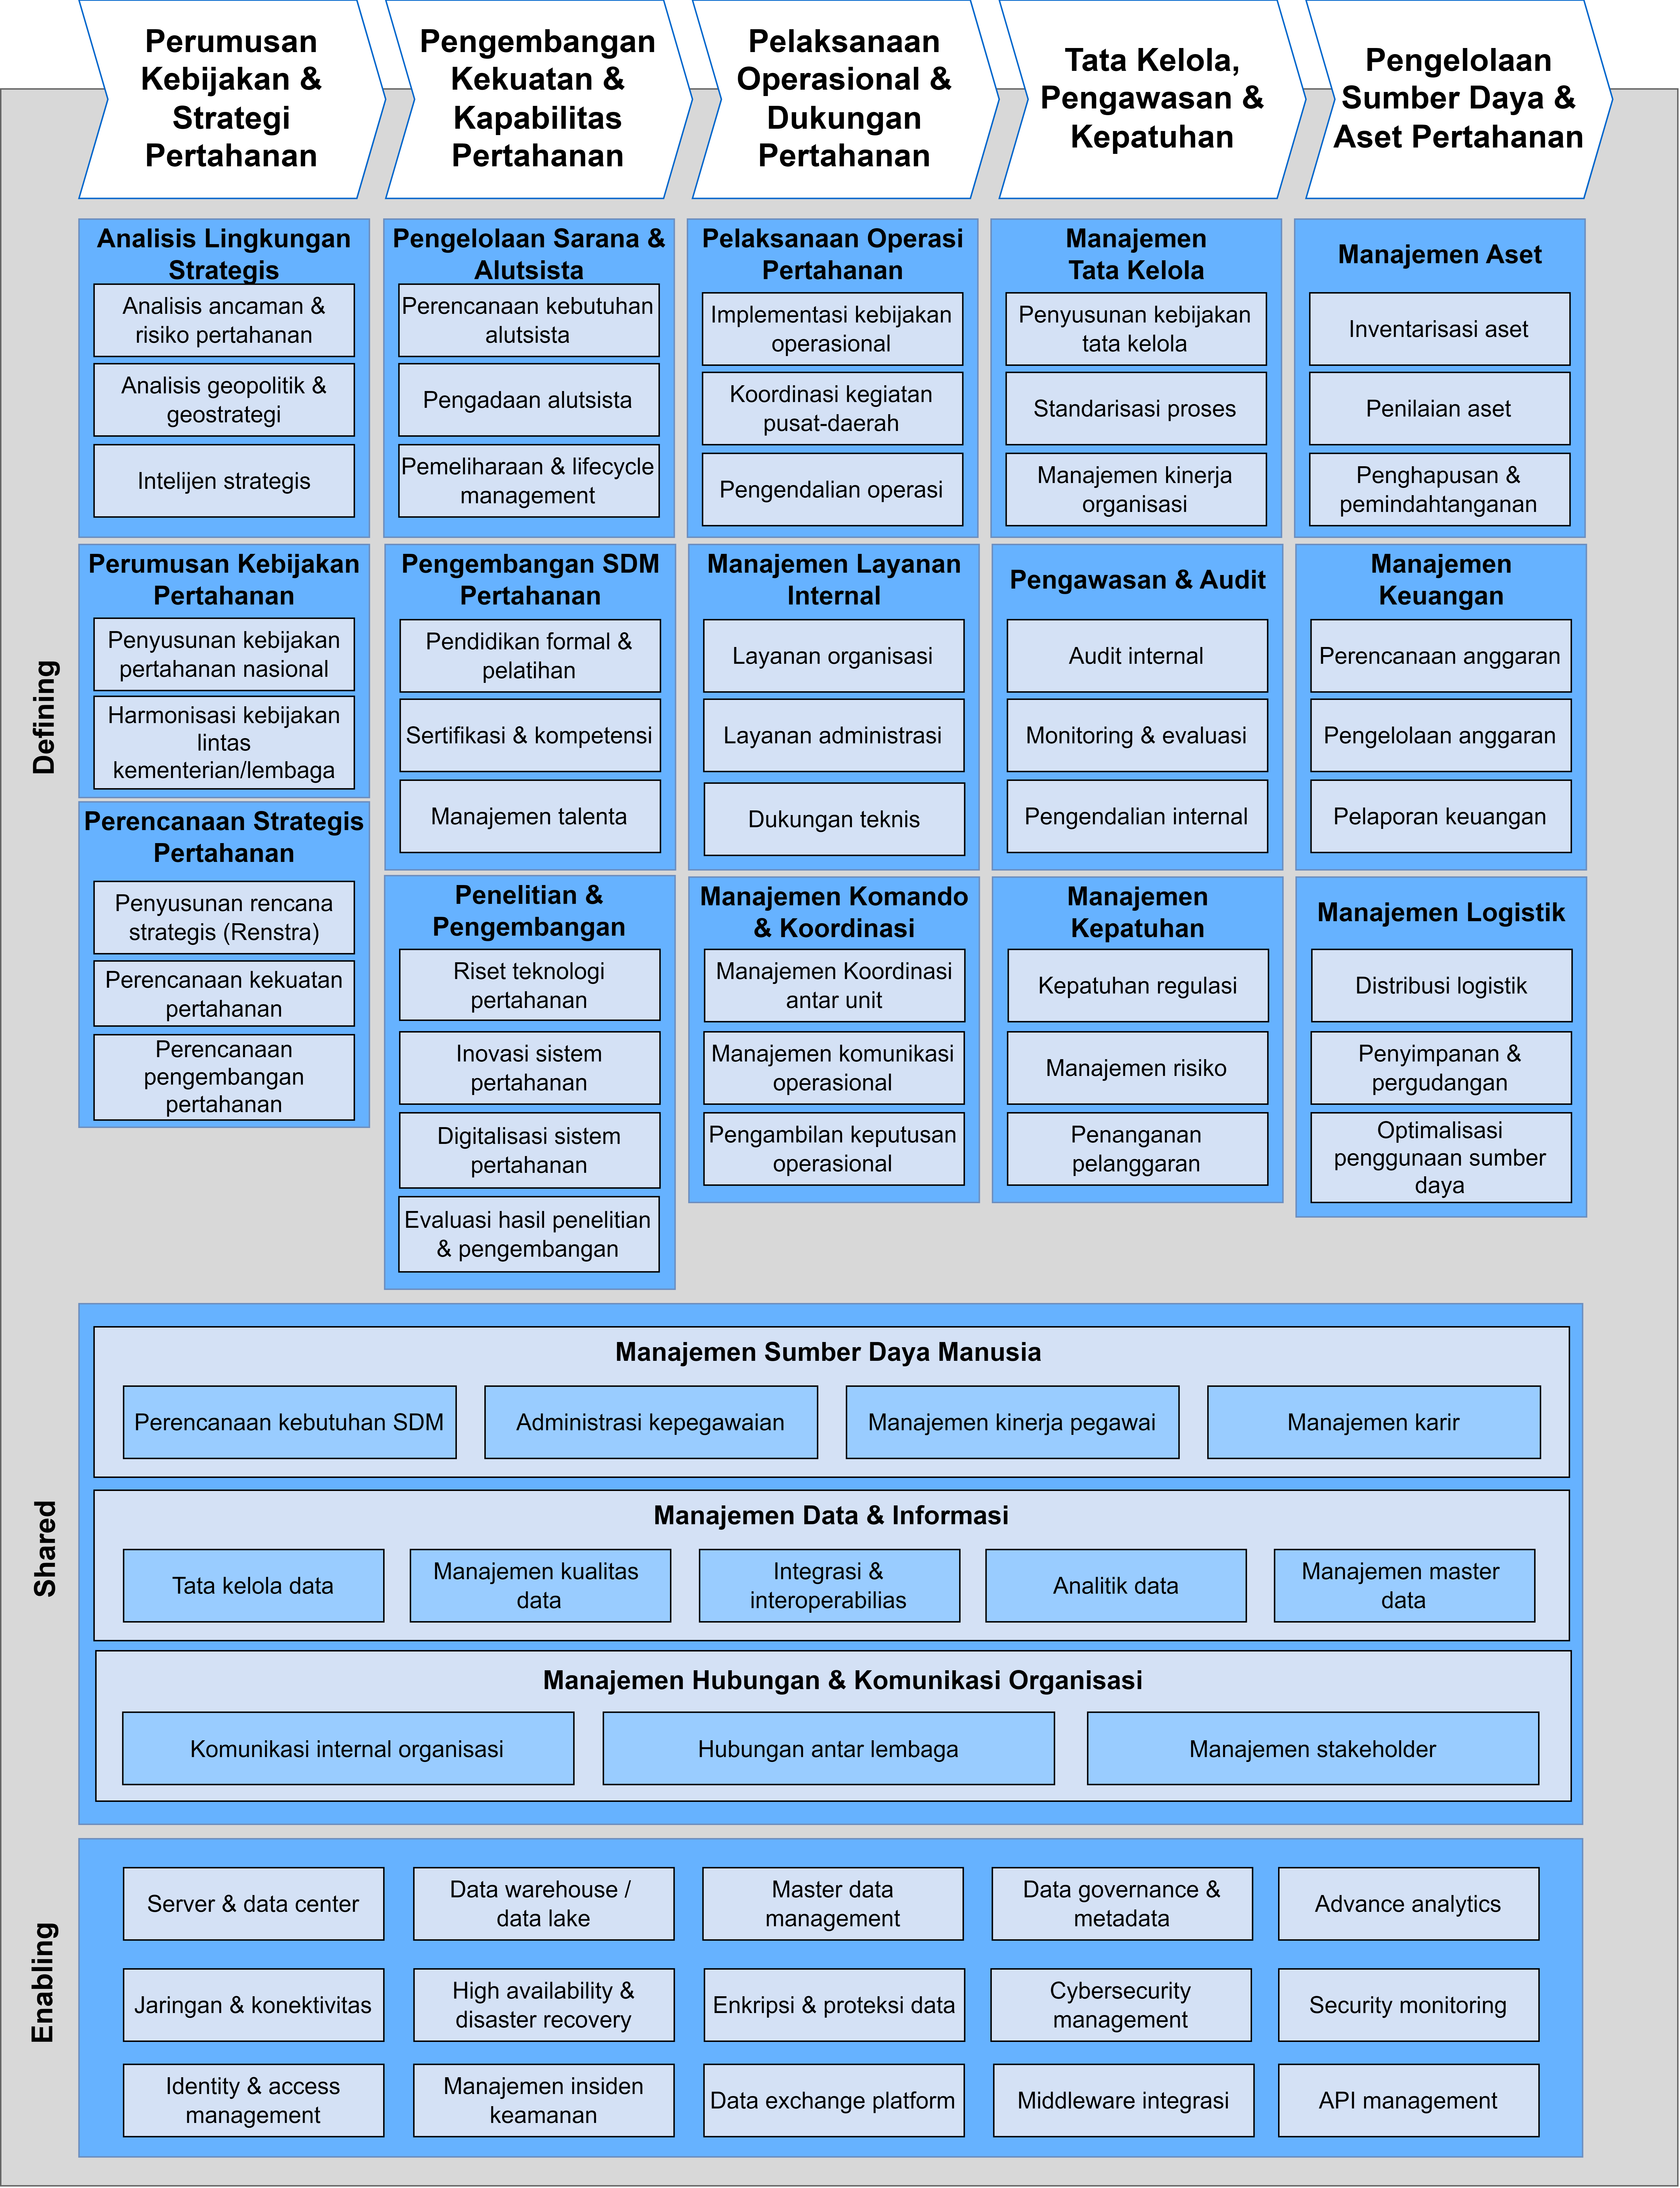
\includegraphics[width=0.93\linewidth,height=0.8\textheight,keepaspectratio]{images/Value Stream & Business Capability Map Kemhan.drawio.png}
\caption{\textit{Business Capability Map} Kemhan RI}
\label{fig:IV.5}
\end{figure}

Gambar~\ref{fig:IV.5} menyusun kapabilitas ke dalam tiga lapis. Lapis \textit{defining} memuat kapabilitas inti yang selaras dengan kelima aliran nilai, mulai dari analisis lingkungan strategis dan perumusan kebijakan hingga manajemen aset, keuangan, dan logistik. Lapis \textit{shared} memuat kapabilitas lintas fungsi, yaitu manajemen sumber daya manusia, manajemen data dan informasi, serta manajemen hubungan dan komunikasi organisasi. Lapis \textit{enabling} memuat fondasi teknologi, meliputi pusat data dan jaringan, pengelolaan data, keamanan siber, serta integrasi melalui \textit{data exchange platform}, \textit{middleware}, dan manajemen API.

\subsection{Arsitektur Bisnis Target}
\label{sec:IV.3.4}

Analisis atas struktur \textit{baseline}, aliran nilai, dan peta kapabilitas menunjukkan bahwa kapabilitas manajemen data dan informasi pada lapis \textit{shared} serta kapabilitas teknologi pada lapis \textit{enabling} belum memiliki pengampu yang mengoordinasikannya lintas organisasi. Oleh karena itu, arsitektur bisnis target difokuskan pada penambahan fungsi yang memimpin transformasi digital pertahanan.

\subsubsection{Struktur Organisasi \textit{To-Be}}
\label{sec:IV.3.4.1}

Berdasarkan Gambar~\ref{fig:IV.3} dan Gambar~\ref{fig:IV.5}, terdapat lima fungsi strategis transformasi digital yang belum memiliki penanggung jawab, yaitu:
\begin{enumerate}[label=\arabic*.]
\item Perumusan strategi dan \textit{roadmap} transformasi digital pertahanan;
\item Tata kelola arsitektur \textit{enterprise} serta standardisasi sistem lintas unit dan lintas matra;
\item Koordinasi transformasi digital lintas satuan kerja dan lintas matra;
\item Tata kelola data sebagai aset strategis, melampaui pengelolaan data yang bersifat operasional; dan
\item Pengkajian dan adopsi teknologi baru (\textit{emerging technology}), seperti kecerdasan buatan dan komputasi awan.
\end{enumerate}

Kelima fungsi tersebut diampu oleh unit \textit{Digital Transformation Officer} (DTO) yang dipimpin CDTO. Unit ini ditempatkan pada tingkat strategis dan bertanggung jawab langsung kepada Menteri Pertahanan. Kedudukan ini memberikan kewenangan lintas eselon I dan lintas matra, memisahkan DTO dari fungsi operasional Pusat Data dan Informasi, serta memungkinkan CDTO memimpin \textit{Architecture Board}. Struktur organisasi target disajikan pada Gambar~\ref{fig:IV.6}.
\begin{figure}[htbp]
\centering
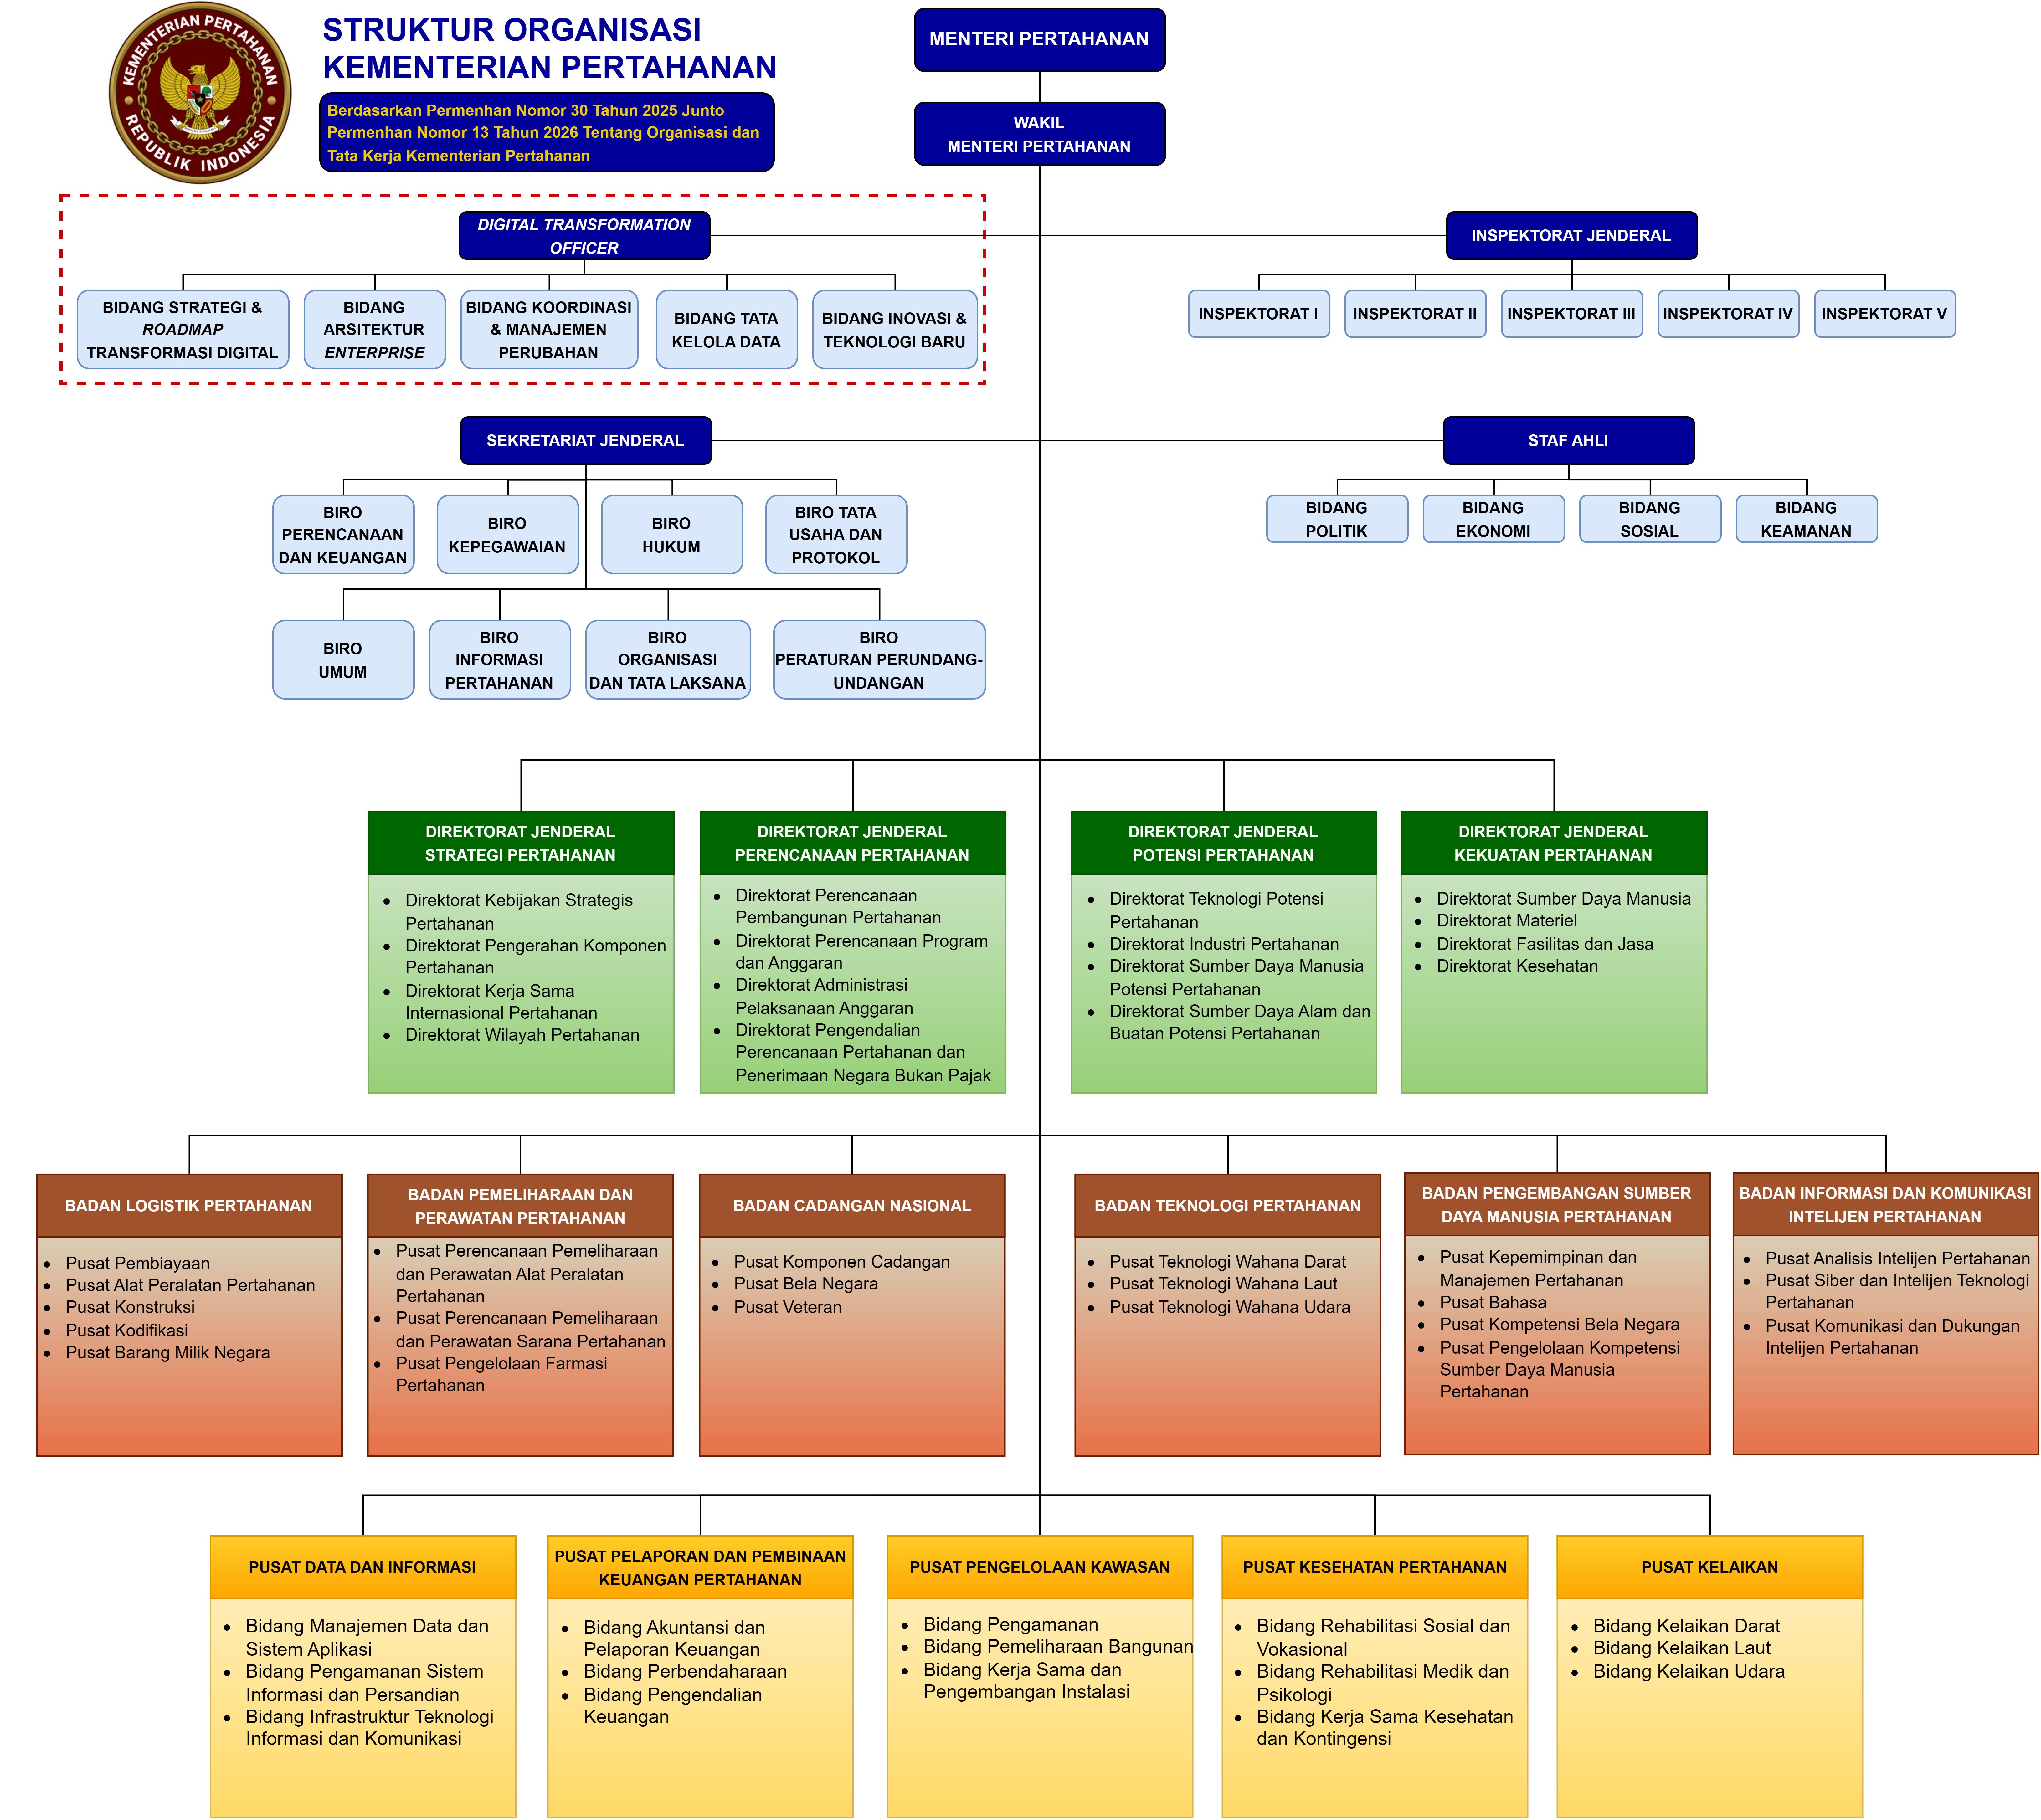
\includegraphics[width=0.99\linewidth,height=0.8\textheight,keepaspectratio]{images/Struktur Organisasi Kemhan Permenhan 30_2025 dan 13_2026 To Be.drawio.png}
\caption{Struktur Organisasi \textit{To-Be} Kemhan RI}
\label{fig:IV.6}
\end{figure}

Gambar~\ref{fig:IV.6} menunjukkan unit DTO (kotak bergaris putus merah) yang berkedudukan langsung di bawah Menteri Pertahanan. Unit ini dipimpin CDTO dan terdiri atas lima bidang yang masing-masing mengampu satu fungsi strategis di atas, yaitu:
\begin{enumerate}[label=\arabic*.]
\item Bidang Strategi dan \textit{Roadmap} Transformasi Digital, merumuskan strategi dan \textit{roadmap} transformasi digital pertahanan, menyelaraskannya dengan rencana strategis Kemhan, serta memantau capaiannya.
\item Bidang Arsitektur \textit{Enterprise}, menyelenggarakan tata kelola arsitektur, menetapkan standar sistem lintas unit dan lintas matra, serta menyiapkan bahan keputusan \textit{Architecture Board}. Bidang ini berisi arsitek setiap domain, yaitu bisnis, data, aplikasi, teknologi, dan C6ISR.
\item Bidang Koordinasi dan Manajemen Perubahan, mengoordinasikan pelaksanaan transformasi lintas satuan kerja dan lintas matra, serta mengelola komunikasi dan kesiapan organisasi dalam menerima perubahan.
\item Bidang Tata Kelola Data, menetapkan kebijakan, standar, dan kepemilikan data pertahanan sebagai aset strategis, sedangkan pengelolaan teknisnya tetap dilaksanakan oleh Pusat Data dan Informasi selaku Walidata Pertahanan.
\item Bidang Inovasi dan Teknologi Baru, yang mengkaji teknologi baru, serta menyiapkan adopsinya melalui uji coba terbatas sebelum diterapkan secara luas.
\end{enumerate}

DTO menetapkan arah strategi dan arsitektur, sedangkan Pusat Data dan Informasi tetap menjadi pelaksana di bidang data, sistem informasi, dan infrastruktur TIK, dengan dukungan Pusat Siber dan Intelijen Teknologi Pertahanan pada aspek siber. Dengan demikian, DTO memperkuat, bukan menggantikan, unit yang telah ada.

\subsubsection{Peta Kapabilitas \textit{To-Be}}
\label{sec:IV.3.4.2}

Peta kapabilitas target (\textit{to-be}) merupakan pemutakhiran atas peta kapabilitas kondisi saat ini (Gambar~\ref{fig:IV.5}) dengan menambahkan kapabilitas baru yang diperlukan untuk mewujudkan arsitektur bisnis target. Karena bersifat lintas fungsi, seluruh kapabilitas baru ditempatkan pada lapis \textit{shared}, sebagaimana disajikan pada Gambar~\ref{fig:IV.7}.
\begin{figure}[htbp]
\centering
\includegraphics[width=0.93\linewidth,height=0.8\textheight,keepaspectratio]{images/Value Stream & Business Capability Map Kemhan To-Be.drawio.png}
\caption{\textit{Business Capability Map} Kemhan RI \textit{To-Be}}
\label{fig:IV.7}
\end{figure}

Gambar~\ref{fig:IV.7} menunjukkan tiga tambahan kapabilitas yang ditandai warna hijau, yaitu:
\begin{enumerate}[label=\arabic*.]
\item Tata Kelola Arsitektur \textit{Enterprise}, yang mencakup manajemen arsitektur \textit{enterprise}, standardisasi dan integrasi sistem, serta \textit{architecture governance} melalui \textit{Architecture Board};
\item Manajemen Perubahan, yang mencakup manajemen perubahan organisasi, adopsi dan komunikasi perubahan, serta kesiapan transformasi; dan
\item Manajemen Talenta Digital, sebagai subkapabilitas Manajemen Sumber Daya Manusia yang dibedakan dari manajemen talenta pertahanan pada lapis \textit{defining}.
\end{enumerate}

\subsubsection{Analisis Kesenjangan}
\label{sec:IV.3.4.3}

Analisis kesenjangan membandingkan kondisi \textit{baseline} dengan arsitektur bisnis target. Hasilnya disajikan pada Tabel~\ref{tab:IV.11}.

\begingroup\small\setstretch{1.0}
\begin{longtable}{@{}>{\raggedright\arraybackslash\hspace{0pt}}p{0.063\linewidth}>{\raggedright\arraybackslash\hspace{0pt}}p{0.157\linewidth}>{\raggedright\arraybackslash\hspace{0pt}}p{0.219\linewidth}>{\raggedright\arraybackslash\hspace{0pt}}p{0.219\linewidth}>{\raggedright\arraybackslash\hspace{0pt}}p{0.219\linewidth}@{}}
\caption{Analisis Kesenjangan Arsitektur Bisnis}\label{tab:IV.11}\\
\toprule
\textbf{No.} & \textbf{Aspek} & \textbf{Kondisi \textit{Baseline}} & \textbf{Kondisi Target} & \textbf{Tindak Lanjut}\\
\midrule
\endfirsthead
\multicolumn{5}{@{}l}{\small\itshape \tablename\ \thetable{} (lanjutan)}\\
\toprule
\textbf{No.} & \textbf{Aspek} & \textbf{Kondisi \textit{Baseline}} & \textbf{Kondisi Target} & \textbf{Tindak Lanjut}\\
\midrule
\endhead
\bottomrule
\endlastfoot
\centering\arraybackslash 1 & Struktur dan mandat transformasi & Belum ada unit bermandat transformasi digital lintas organisasi & Unit DTO pada tingkat strategis dengan lima bidang & Pembentukan unit DTO\\
\centering\arraybackslash 2 & Tata kelola arsitektur & Belum ada tata kelola arsitektur \textit{enterprise} dan standar lintas unit & Kapabilitas Tata Kelola Arsitektur \textit{Enterprise} dan \textit{Architecture Board} & Penetapan tata kelola dan standar arsitektur\\
\centering\arraybackslash 3 & Manajemen perubahan & Transformasi berjalan parsial tanpa pengelolaan perubahan & Kapabilitas Manajemen Perubahan yang terlembaga & Pembangunan kapabilitas manajemen perubahan\\
\centering\arraybackslash 4 & Proses bisnis lintas unit & Proses terfragmentasi dan belum terstandar antarunit & Proses terstandar dan terintegrasi berbasis kapabilitas & Standardisasi dan integrasi proses bisnis\\
\centering\arraybackslash 5 & Koordinasi lintas matra & Koordinasi antarunit dan antarmatra bersifat \textit{ad hoc} & Mekanisme koordinasi transformasi lintas matra yang terlembaga & Penetapan mekanisme koordinasi lintas matra\\
\centering\arraybackslash 6 & Talenta digital & Kompetensi digital terbatas dan tersebar antarunit & Kapabilitas Manajemen Talenta Digital & Pengembangan dan rekrutmen talenta digital\\
\end{longtable}
\endgroup

Tabel~\ref{tab:IV.11} menunjukkan bahwa kesenjangan 1 dan 2 bersifat struktural sehingga harus ditutup lebih dahulu sebagai prasyarat bagi kesenjangan lainnya.

\subsubsection{\textit{Roadmap} Implementasi}
\label{sec:IV.3.4.4}

\textit{Roadmap} Fase \textit{Business Architecture} menyusun urutan inisiatif untuk menutup kesenjangan pada Tabel~\ref{tab:IV.11} dalam tiga horizon waktu, sebagaimana disajikan pada Gambar~\ref{fig:IV.8}.
\begin{figure}[htbp]
\centering
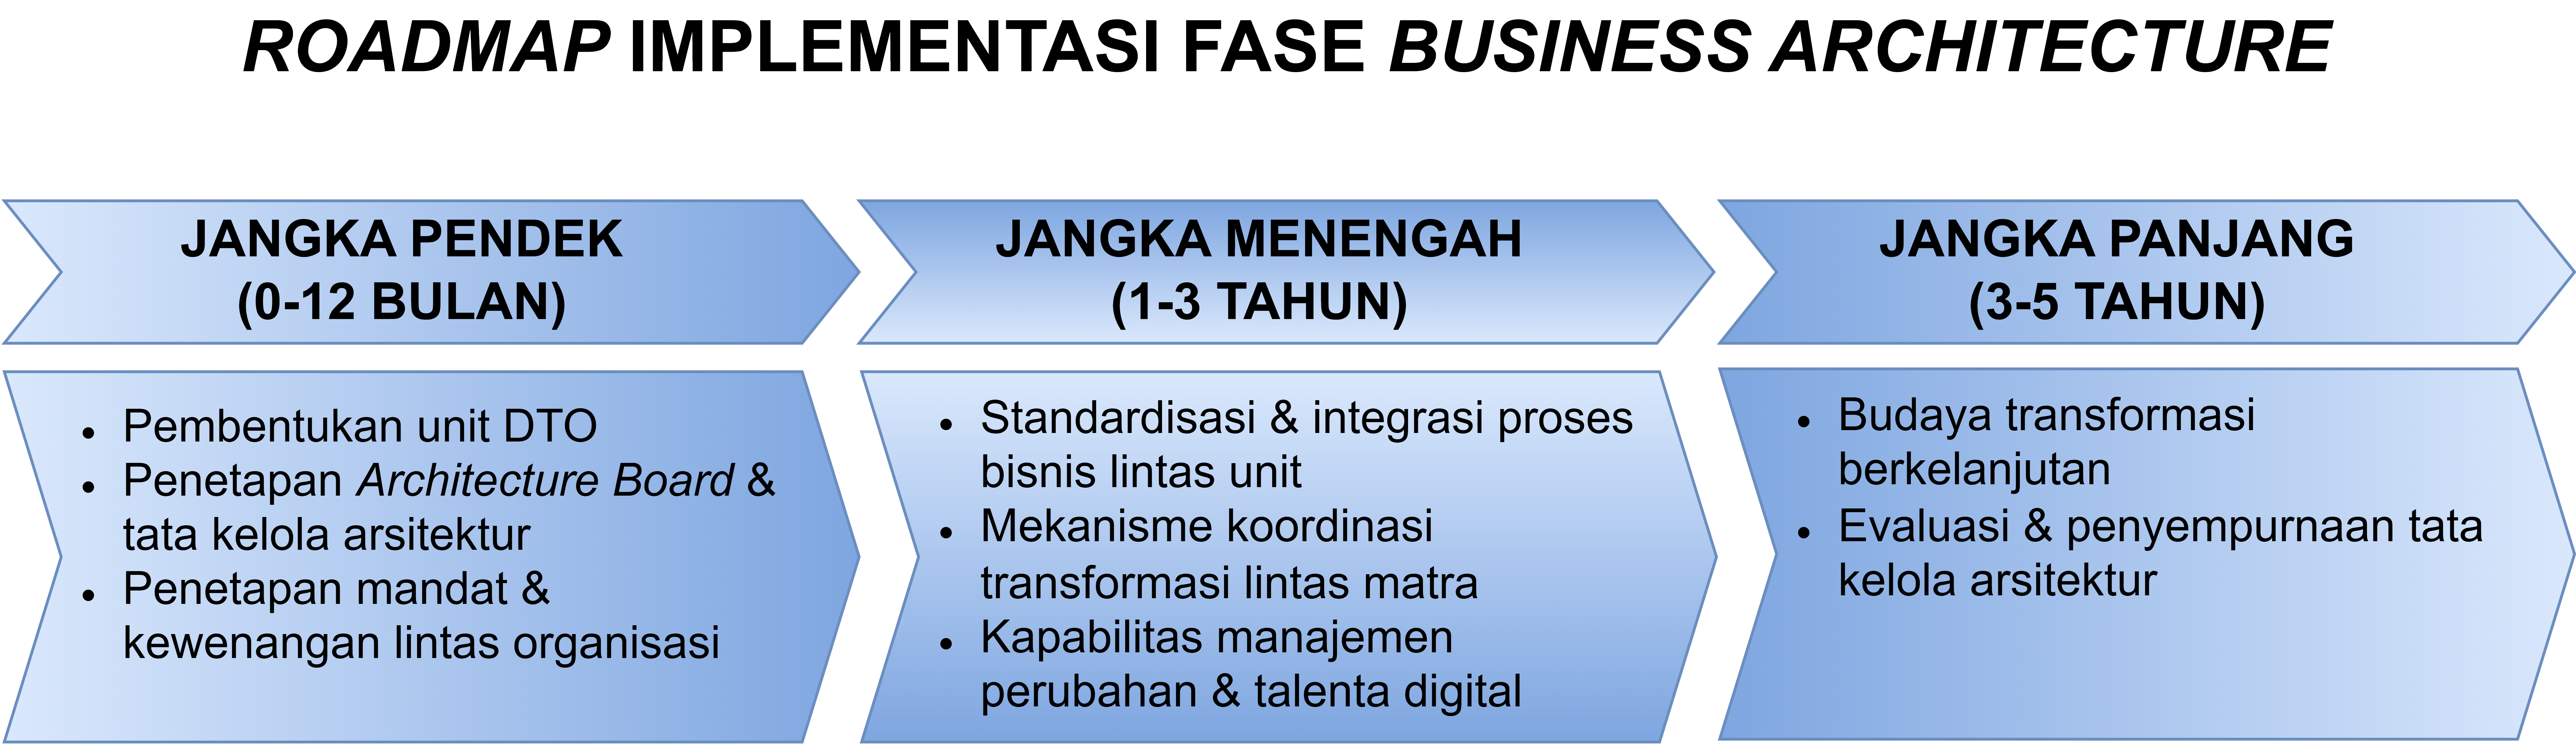
\includegraphics[width=0.99\linewidth,height=0.8\textheight,keepaspectratio]{images/Roadmap implementasi fase business architecture.drawio.png}
\caption{\textit{Roadmap} Implementasi Fase \textit{Business Architecture}}
\label{fig:IV.8}
\end{figure}

Gambar~\ref{fig:IV.8} menunjukkan bahwa jangka pendek (0–12 bulan) difokuskan pada pembentukan unit DTO, \textit{Architecture Board}, serta mandat lintas organisasi untuk menutup kesenjangan 1 dan 2. Jangka menengah (1–3 tahun) menutup kesenjangan 3 hingga 6 melalui standardisasi proses bisnis, mekanisme koordinasi lintas matra, serta kapabilitas manajemen perubahan dan talenta digital. Jangka panjang (3–5 tahun) diarahkan pada budaya transformasi berkelanjutan serta evaluasi dan penyempurnaan tata kelola arsitektur.

Dengan demikian, Fase Business Architecture menghasilkan \textit{value stream}, peta kapabilitas, model tata kelola dan komando, serta mekanisme koordinasi lintas matra.

\section{Fase Information Systems Architecture}
\label{sec:IV.4}

Fase Information Systems Architecture merancang arsitektur data dan arsitektur aplikasi yang mendukung proses bisnis pertahanan. Sesuai Tabel~\ref{tab:III.10} dan Tabel~\ref{tab:III.11}, arsitektur data dikerjakan lebih dahulu, kemudian arsitektur aplikasi. Keduanya bertolak dari inventarisasi aplikasi Kemhan tahun 2025 yang mencatat 247 aplikasi, terdiri atas 176 aplikasi umum dan 71 aplikasi khusus, sebagaimana direkapitulasi pada Tabel~\ref{tab:IV.12}.

\begingroup\small\setstretch{1.0}
\begin{longtable}{@{}>{\raggedright\arraybackslash\hspace{0pt}}p{0.063\linewidth}>{\raggedright\arraybackslash\hspace{0pt}}p{0.501\linewidth}>{\raggedright\arraybackslash\hspace{0pt}}p{0.104\linewidth}>{\raggedright\arraybackslash\hspace{0pt}}p{0.104\linewidth}>{\raggedright\arraybackslash\hspace{0pt}}p{0.104\linewidth}@{}}
\caption{Rekapitulasi Aplikasi \textit{Baseline} per Satuan Kerja}\label{tab:IV.12}\\
\toprule
\textbf{No.} & \textbf{Satuan Kerja} & \textbf{Umum} & \textbf{Khusus} & \textbf{Jumlah}\\
\midrule
\endfirsthead
\multicolumn{5}{@{}l}{\small\itshape \tablename\ \thetable{} (lanjutan)}\\
\toprule
\textbf{No.} & \textbf{Satuan Kerja} & \textbf{Umum} & \textbf{Khusus} & \textbf{Jumlah}\\
\midrule
\endhead
\bottomrule
\endlastfoot
\centering\arraybackslash 1 & Ditjen Strategi Pertahanan & \centering\arraybackslash 10 & \centering\arraybackslash 0 & \centering\arraybackslash 10\\
\centering\arraybackslash 2 & Ditjen Perencanaan Pertahanan & \centering\arraybackslash 22 & \centering\arraybackslash 0 & \centering\arraybackslash 22\\
\centering\arraybackslash 3 & Ditjen Potensi Pertahanan & \centering\arraybackslash 8 & \centering\arraybackslash 4 & \centering\arraybackslash 12\\
\centering\arraybackslash 4 & Ditjen Kekuatan Pertahanan & \centering\arraybackslash 21 & \centering\arraybackslash 0 & \centering\arraybackslash 21\\
\centering\arraybackslash 5 & Inspektorat Jenderal & \centering\arraybackslash 2 & \centering\arraybackslash 1 & \centering\arraybackslash 3\\
\centering\arraybackslash 6 & Biro Perencanaan dan Keuangan & \centering\arraybackslash 2 & \centering\arraybackslash 0 & \centering\arraybackslash 2\\
\centering\arraybackslash 7 & Biro Kepegawaian & \centering\arraybackslash 2 & \centering\arraybackslash 4 & \centering\arraybackslash 6\\
\centering\arraybackslash 8 & Biro Hukum & \centering\arraybackslash 0 & \centering\arraybackslash 1 & \centering\arraybackslash 1\\
\centering\arraybackslash 9 & Biro Tata Usaha dan Protokol & \centering\arraybackslash 16 & \centering\arraybackslash 0 & \centering\arraybackslash 16\\
\centering\arraybackslash 10 & Biro Umum & \centering\arraybackslash 17 & \centering\arraybackslash 0 & \centering\arraybackslash 17\\
\centering\arraybackslash 11 & Biro Informasi Pertahanan & \centering\arraybackslash 0 & \centering\arraybackslash 2 & \centering\arraybackslash 2\\
\centering\arraybackslash 12 & Biro Organisasi dan Tata Laksana & \centering\arraybackslash 0 & \centering\arraybackslash 1 & \centering\arraybackslash 1\\
\centering\arraybackslash 13 & Biro Peraturan Perundang-undangan & \centering\arraybackslash 1 & \centering\arraybackslash 0 & \centering\arraybackslash 1\\
\centering\arraybackslash 14 & Badan Logistik Pertahanan & \centering\arraybackslash 5 & \centering\arraybackslash 1 & \centering\arraybackslash 6\\
\centering\arraybackslash 15 & Badan Teknologi Pertahanan & \centering\arraybackslash 18 & \centering\arraybackslash 1 & \centering\arraybackslash 19\\
\centering\arraybackslash 16 & Badan Pengembangan Sumber Daya Manusia Pertahanan & \centering\arraybackslash 0 & \centering\arraybackslash 27 & \centering\arraybackslash 27\\
\centering\arraybackslash 17 & Pusat Data dan Informasi & \centering\arraybackslash 6 & \centering\arraybackslash 8 & \centering\arraybackslash 14\\
\centering\arraybackslash 18 & Badan Informasi dan Komunikasi Intelijen Pertahanan & \centering\arraybackslash 0 & \centering\arraybackslash 16 & \centering\arraybackslash 16\\
\centering\arraybackslash 19 & Pusat Kelaikan & \centering\arraybackslash 13 & \centering\arraybackslash 0 & \centering\arraybackslash 13\\
\centering\arraybackslash 20 & Pusat Kesehatan Pertahanan & \centering\arraybackslash 14 & \centering\arraybackslash 4 & \centering\arraybackslash 18\\
\centering\arraybackslash 21 & Pusat Pelaporan dan Pembinaan Keuangan Pertahanan & \centering\arraybackslash 12 & \centering\arraybackslash 1 & \centering\arraybackslash 13\\
\centering\arraybackslash 22 & Universitas Pertahanan & \centering\arraybackslash 7 & \centering\arraybackslash 0 & \centering\arraybackslash 7\\
 & \textbf{Total} & \centering\arraybackslash \textbf{176} & \centering\arraybackslash \textbf{71} & \centering\arraybackslash \textbf{247}\\
\end{longtable}
\endgroup

Tabel~\ref{tab:IV.12} menunjukkan bahwa aplikasi khusus terkonsentrasi pada Badan Pengembangan Sumber Daya Manusia Pertahanan (27 aplikasi), Badan Informasi dan Komunikasi Intelijen Pertahanan (16 aplikasi), dan Pusat Data dan Informasi (8 aplikasi).

\subsection{Data Architecture}
\label{sec:IV.4.1}

Arsitektur data merancang definisi, klasifikasi, dan kepemilikan Data Pertahanan. Menurut Permenhan Nomor 1 Tahun 2023 \cite{Permenhan1Tahun2023}, Data Pertahanan adalah data yang dibina dan diselenggarakan oleh Kemhan dan TNI untuk kepentingan penyelenggaraan pertahanan negara. Perancangan berpedoman pada prinsip \textit{Data as Strategic Asset} serta empat prinsip Satu Data, yaitu standar data, metadata, interoperabilitas data, serta kode referensi dan data induk.

\subsubsection{Arsitektur Data Baseline}
\label{sec:IV.4.1.1}

Aplikasi umum pada Tabel~\ref{tab:IV.12} merupakan sistem nasional yang digunakan bersama oleh banyak instansi, seperti SAKTI, SIMPEG, SIRUP, KRISNA, dan OM-SPAN. Kemhan berkedudukan sebagai pengguna, sehingga data aplikasi tersebut tunduk pada tata kelola instansi penyelenggaranya dan berada di luar lingkup arsitektur data Kemhan. Sebaliknya, 71 aplikasi khusus dibina dan diselenggarakan sendiri oleh Kemhan, sehingga datanya merupakan Data Pertahanan dan menjadi lingkup arsitektur data serta Satu Data Pertahanan.

Pada kondisi \textit{baseline}, Data Pertahanan masih terkotak per aplikasi dan per satuan kerja. Data tersebut belum memiliki kamus data, klasifikasi, maupun kanal berbagi-pakai.

\subsubsection{Model Entitas Data Pertahanan}
\label{sec:IV.4.1.2}

Entitas data diturunkan dari fungsi 71 aplikasi khusus, kemudian dikelompokkan ke dalam empat domain. Daftar entitas utama Data Pertahanan disajikan pada Tabel~\ref{tab:IV.13}.

\begingroup\small\setstretch{1.0}
\begin{longtable}{@{}>{\raggedright\arraybackslash\hspace{0pt}}p{0.065\linewidth}>{\raggedright\arraybackslash\hspace{0pt}}p{0.233\linewidth}>{\raggedright\arraybackslash\hspace{0pt}}p{0.259\linewidth}>{\raggedright\arraybackslash\hspace{0pt}}p{0.350\linewidth}@{}}
\caption{Entitas Data Pertahanan}\label{tab:IV.13}\\
\toprule
\textbf{No.} & \textbf{Entitas Data} & \textbf{Aplikasi Sumber} & \textbf{Deskripsi}\\
\midrule
\endfirsthead
\multicolumn{4}{@{}l}{\small\itshape \tablename\ \thetable{} (lanjutan)}\\
\toprule
\textbf{No.} & \textbf{Entitas Data} & \textbf{Aplikasi Sumber} & \textbf{Deskripsi}\\
\midrule
\endhead
\bottomrule
\endlastfoot
\multicolumn{4}{@{}>{\raggedright\arraybackslash\hspace{0pt}}p{0.997\linewidth}@{}}{\textbf{Kepegawaian, Hukum, dan Pengawasan}}\\
\centering\arraybackslash 1 & Data Kinerja Pegawai & E-Kinerja, E-LAPKIN & Capaian dan laporan kinerja pegawai serta organisasi\\
\centering\arraybackslash 2 & Data Kompetensi dan Asesmen & SIAC & Hasil asesmen kompetensi dan pemetaan talenta pegawai\\
\centering\arraybackslash 3 & Data Kartu Identitas Pegawai & E-KTA, SiUdin & Identitas resmi dan kartu tanda anggota pegawai\\
\centering\arraybackslash 4 & Data Perkara dan Dokumentasi Hukum & Si Rokum & Perkara, pendapat hukum, dan dokumentasi produk hukum\\
\centering\arraybackslash 5 & Data Pengawasan Intern & SIMWAS & Temuan, rekomendasi, dan tindak lanjut pengawasan intern\\
\multicolumn{4}{@{}>{\raggedright\arraybackslash\hspace{0pt}}p{0.997\linewidth}@{}}{\textbf{Layanan Publik dan Potensi Pertahanan}}\\
\centering\arraybackslash 6 & Data Layanan Informasi Publik & E-PPID, Smart Mobile Reporting & Permohonan informasi publik\\
\centering\arraybackslash 7 & Data Veteran & Veteran & Identitas, status, dan hak veteran\\
\centering\arraybackslash 8 & Data Sumber Daya dan Industri Pertahanan & Sisinfo Sumdahan, Daya Serap & Potensi sumber daya nasional dan kapasitas industri pertahanan\\
\centering\arraybackslash 9 & Data Perizinan Pertahanan & Perizinan & Permohonan dan penerbitan izin industri pertahanan\\
\multicolumn{4}{@{}>{\raggedright\arraybackslash\hspace{0pt}}p{0.997\linewidth}@{}}{\textbf{Pendidikan, Kesehatan, Litbang, dan Keuangan}}\\
\centering\arraybackslash 10 & Data Peserta Didik dan Akademik & Aplikasi Pengelolaan Siswa/Akademik, Sistem Layanan Diklat & Peserta didik, kurikulum, jadwal, dan nilai akademik\\
\centering\arraybackslash 11 & Data Alumni & Sistem Pengelolaan Alumni & Riwayat dan penelusuran alumni pendidikan pertahanan\\
\centering\arraybackslash 12 & Data Bahan Ajar dan Pembelajaran Digital & Bahan Ajar Digital, VR Diklat, Sistem Pembelajaran Elektronik & Materi ajar, modul, dan konten pembelajaran digital\\
\centering\arraybackslash 13 & Data Rekam Medis dan Pasien & SimRS, Sismadak & Rekam medis, riwayat layanan, dan mutu pelayanan pasien\\
\centering\arraybackslash 14 & Data Klaim Layanan Kesehatan & E-Klaim & Pengajuan dan verifikasi klaim layanan kesehatan\\
\centering\arraybackslash 15 & Data Penelitian dan Pengembangan & Data Digital Arsip Penelitian & Arsip hasil penelitian dan pengembangan pertahanan\\
\centering\arraybackslash 16 & Data Pelaporan Keuangan Internal & EMINU & Pelaporan dan pemantauan keuangan internal\\
\multicolumn{4}{@{}>{\raggedright\arraybackslash\hspace{0pt}}p{0.997\linewidth}@{}}{\textbf{Data Strategis, Geospasial, dan Keamanan Siber}}\\
\centering\arraybackslash 17 & Data Geospasial Wilayah Pertahanan & Peta Tematik Wilayah Pertahanan, Layanan Peta Digital, IGD Sumdahan & Peta tematik dan data spasial wilayah serta objek pertahanan\\
\centering\arraybackslash 18 & Data Log dan Insiden Keamanan Siber & SIEM, Splunk, Honeypot, Log Manajemen & Aktivitas, deteksi, dan penanganan insiden siber\\
\centering\arraybackslash 19 & Data Identitas dan Kendali Akses & Single Sign On (SSO), Access Control & Identitas pengguna, hak akses, dan otentikasi sistem\\
\centering\arraybackslash 20 & Data Aset dan Infrastruktur TIK & Rack Management, EMS, The Dude, Cacti & Inventaris dan kondisi perangkat, jaringan, serta infrastruktur TIK\\
\end{longtable}
\endgroup

Tabel~\ref{tab:IV.13} menunjukkan bahwa satu entitas dapat bersumber dari lebih dari satu aplikasi. Oleh karena itu, kamus data dan data induk diperlukan agar entitas yang sama tidak direkam secara berbeda.

\subsubsection{Klasifikasi Data}
\label{sec:IV.4.1.3}

Klasifikasi data diperlukan untuk menyeimbangkan kewajiban berbagi-pakai data dengan kewajiban kerahasiaan pertahanan. Sesuai Pasal 21 Permenhan Nomor 1 Tahun 2023 \cite{Permenhan1Tahun2023}, Data Pertahanan diklasifikasikan ke dalam tiga tingkat sebagaimana disajikan pada Tabel~\ref{tab:IV.14}.

\begingroup\small\setstretch{1.0}
\begin{longtable}{@{}>{\raggedright\arraybackslash\hspace{0pt}}p{0.187\linewidth}>{\raggedright\arraybackslash\hspace{0pt}}p{0.401\linewidth}>{\raggedright\arraybackslash\hspace{0pt}}p{0.348\linewidth}@{}}
\caption{Klasifikasi Data Pertahanan}\label{tab:IV.14}\\
\toprule
\textbf{Klasifikasi} & \textbf{Kriteria} & \textbf{Kendali Akses}\\
\midrule
\endfirsthead
\multicolumn{3}{@{}l}{\small\itshape \tablename\ \thetable{} (lanjutan)}\\
\toprule
\textbf{Klasifikasi} & \textbf{Kriteria} & \textbf{Kendali Akses}\\
\midrule
\endhead
\bottomrule
\endlastfoot
Data Terbuka & Data yang boleh diketahui publik & Terbuka untuk publik melalui Portal Satu Data Pertahanan\\
Data Terbatas & Data yang hanya dapat diakses oleh kementerian/lembaga yang diberi akses oleh Walidata Pertahanan & Otentikasi dan hak akses berbasis izin Walidata Pertahanan\\
Data Rahasia & Data yang hanya dapat diakses oleh pejabat berwenang di Kemhan, Mabes TNI, dan Mabes Angkatan & Otorisasi khusus, enkripsi, dan pencatatan audit\\
\end{longtable}
\endgroup

\subsubsection{Kamus Data dan Standar Penamaan}
\label{sec:IV.4.1.4}

Kamus data (\textit{data dictionary}) memuat definisi baku setiap entitas dan atribut, sedangkan metadata melekat pada setiap set data. Keduanya disusun agar entitas yang sama tidak direkam secara berbeda antaraplikasi. Standar penamaan yang ditetapkan adalah sebagai berikut:
\begin{enumerate}[label=\arabic*.]
\item Nama entitas dan atribut menggunakan bahasa Indonesia baku, deskriptif, dan tanpa singkatan yang ambigu;
\item Penamaan atribut mengikuti pola [entitas]\_[atribut] dengan huruf kecil dan garis bawah (\textit{snake\_case}), misalnya pegawai\_nip dan veteran\_nomor;
\item Setiap entitas memiliki satu pengidentifikasi unik (\textit{primary key}) yang baku, misalnya NIP/NRP untuk pegawai dan nomor registrasi untuk veteran;
\item Setiap entitas dan atribut memiliki satu definisi yang disepakati dan dicatat dalam kamus data; dan
\item Metadata mengikuti struktur Satu Data Indonesia, mencakup definisi, format, satuan, klasifikasi, dan walidata.
\end{enumerate}

\subsubsection{Matriks Kepemilikan data dan Tata Kelola Data}
\label{sec:IV.4.1.5}

Tata kelola Data Pertahanan mengikuti penyelenggara Satu Data Pertahanan pada Permenhan Nomor 1 Tahun 2023 \cite{Permenhan1Tahun2023}. Pembagian peran tersebut disajikan pada Tabel~\ref{tab:IV.15}.

\begingroup\small\setstretch{1.0}
\begin{longtable}{@{}>{\raggedright\arraybackslash\hspace{0pt}}p{0.221\linewidth}>{\raggedright\arraybackslash\hspace{0pt}}p{0.375\linewidth}>{\raggedright\arraybackslash\hspace{0pt}}p{0.341\linewidth}@{}}
\caption{Peran Penyelenggara Satu Data Pertahanan}\label{tab:IV.15}\\
\toprule
\textbf{Peran} & \textbf{Tugas Pokok} & \textbf{Pemangku Peran}\\
\midrule
\endfirsthead
\multicolumn{3}{@{}l}{\small\itshape \tablename\ \thetable{} (lanjutan)}\\
\toprule
\textbf{Peran} & \textbf{Tugas Pokok} & \textbf{Pemangku Peran}\\
\midrule
\endhead
\bottomrule
\endlastfoot
Pengarah & Mengoordinasikan pelaksanaan, pemantauan, evaluasi, dan pelaporan Satu Data Pertahanan kepada Menteri & Sekretaris Jenderal Kemhan\\
Walidata Pertahanan & Merencanakan, mengumpulkan, memeriksa, mengelola, dan menyebarluaskan data melalui Portal Satu Data Pertahanan & Pusat Data dan Informasi\\
Produsen Data Pertahanan & Menghasilkan data sesuai prinsip Satu Data serta menyampaikan data dan metadata kepada Walidata & Satuan kerja penghasil data di Kemhan dan Mabes TNI\\
Pengolah Data Pertahanan & Mendistribusikan Data Pertahanan hingga sampai kepada Walidata & Satuan kerja pengelola data di Mabes Angkatan\\
Pengaman Sistem Data Pertahanan & Mengamankan, memantau, menguji, dan merespons ancaman siber terhadap sistem Satu Data Pertahanan & Bidang Pengamanan Sistem Informasi dan Persandian, didukung Pusat Siber dan Intelijen Teknologi Pertahanan\\
Forum Satu Data Pertahanan & Wadah komunikasi dan koordinasi penyelenggaraan Satu Data Pertahanan & Walidata, Produsen, Pengolah, dan Pengaman Sistem Data\\
\end{longtable}
\endgroup

Tabel~\ref{tab:IV.15} menunjukkan bahwa setiap Data Pertahanan dihasilkan oleh produsen data di satuan kerja, sedangkan pengelolaan dan penyebarluasannya dipusatkan pada satu Walidata Pertahanan, yaitu Pusat Data dan Informasi \cite{Permenhan30Tahun2025,Permenhan13Tahun2026}. Kebijakan dan standar data ditetapkan oleh Bidang Tata Kelola Data pada unit DTO, kemudian dijalankan oleh Walidata Pertahanan.

\subsubsection{Arsitektur Data Target}
\label{sec:IV.4.1.6}

Arsitektur data target adalah terwujudnya Satu Data Pertahanan, yaitu Data Pertahanan yang terstandar, terklasifikasi, dimiliki secara jelas, aman, dan dapat dibagipakaikan secara terkendali. Arsitektur ini disusun dalam tiga lapis, yaitu fondasi, platform, dan target, sebagaimana ditunjukkan pada Gambar~\ref{fig:IV.9}.
\begin{figure}[htbp]
\centering
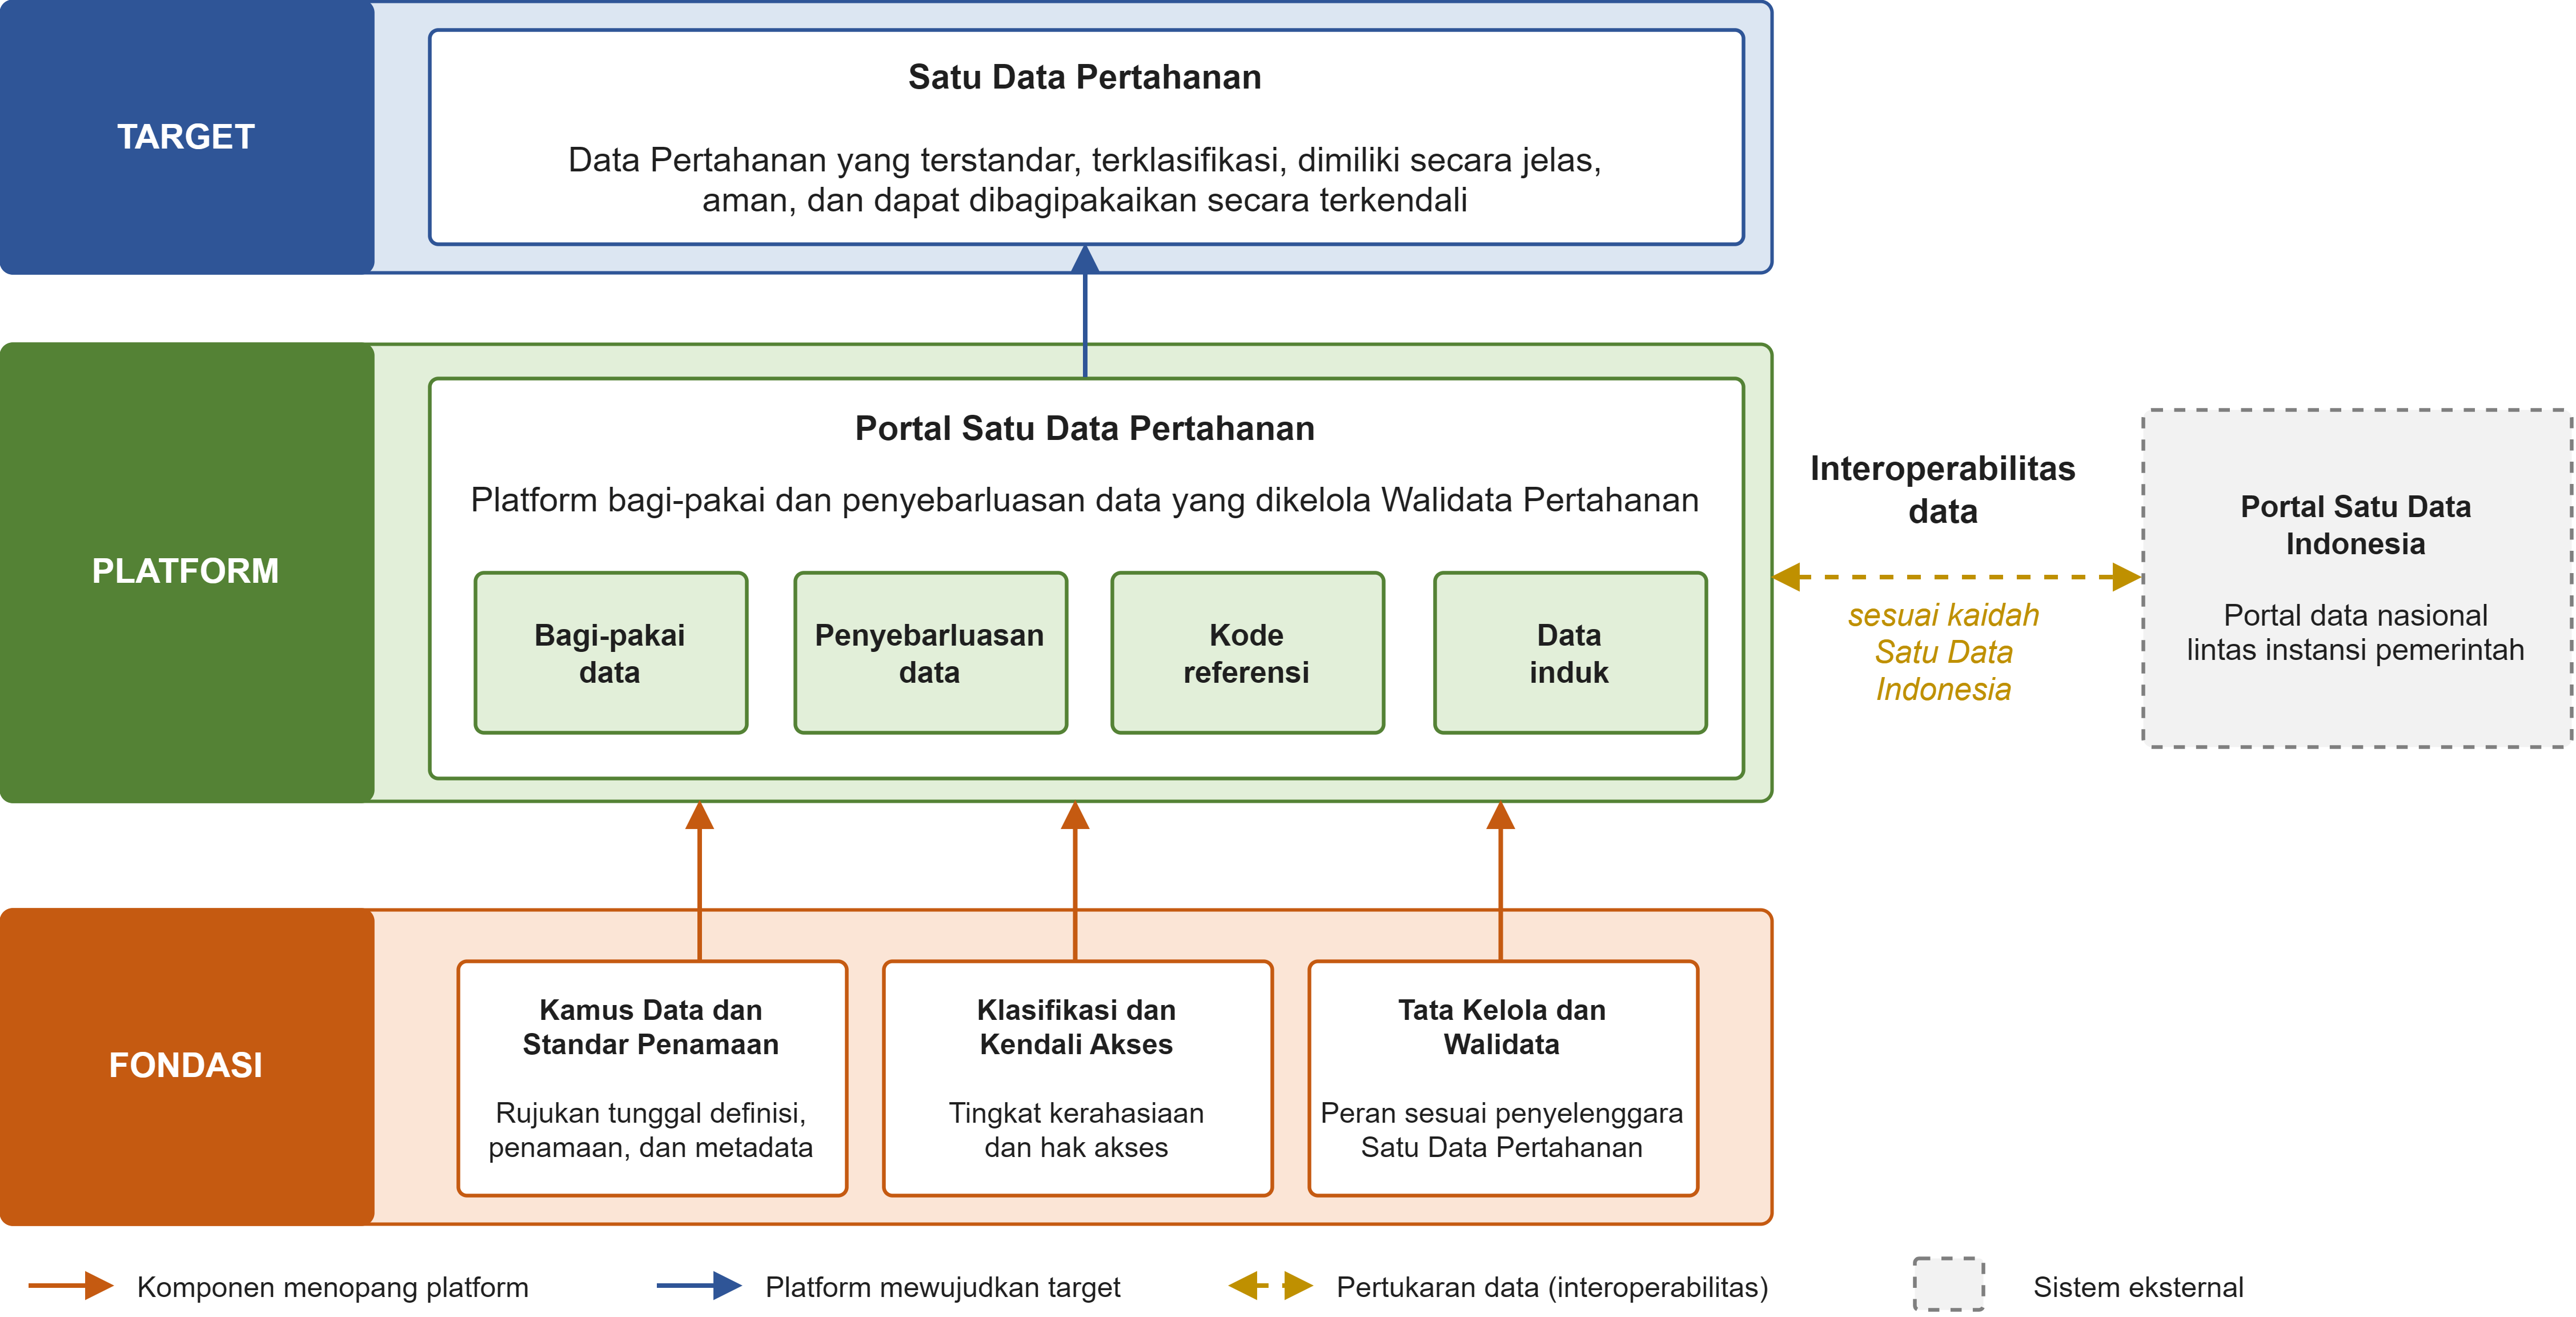
\includegraphics[width=0.99\linewidth,height=0.8\textheight,keepaspectratio]{images/Arsitektur_Data_Target.drawio.png}
\caption{Arsitektur Data Target}
\label{fig:IV.9}
\end{figure}

Gambar~\ref{fig:IV.9} menunjukkan bahwa lapis fondasi terdiri atas tiga komponen, yaitu kamus data dan standar penamaan, klasifikasi dan kendali akses, serta tata kelola dan walidata. Ketiganya menjadi prasyarat Portal Satu Data Pertahanan. Tanpa ketiga komponen tersebut, portal hanya menjadi penampung data yang tidak seragam, tidak terklasifikasi, dan tidak jelas kepemilikannya.

Lapis platform adalah Portal Satu Data Pertahanan yang dikelola Walidata Pertahanan dengan empat fungsi, yaitu bagi-pakai data, penyebarluasan data, kode referensi, dan data induk. Kode referensi dan data induk menjadi acuan bersama bagi aplikasi di Kemhan dan Mabes TNI, sehingga entitas yang sama, seperti pegawai, veteran, dan alat peralatan pertahanan, tidak lagi direkam secara berbeda. Portal ini terhubung dua arah dengan Portal Satu Data Indonesia sesuai kaidah Satu Data Indonesia, tetapi hanya untuk data yang klasifikasinya memungkinkan. Data Rahasia tetap berada di lingkungan internal pertahanan.

\subsubsection{Analisis Kesenjangan}
\label{sec:IV.4.1.7}

Analisis kesenjangan arsitektur data membandingkan kondisi \textit{baseline} dengan arsitektur data target pada enam aspek, sebagaimana disajikan pada Tabel~\ref{tab:IV.16}.

\begingroup\small\setstretch{1.0}
\begin{longtable}{@{}>{\raggedright\arraybackslash\hspace{0pt}}p{0.063\linewidth}>{\raggedright\arraybackslash\hspace{0pt}}p{0.157\linewidth}>{\raggedright\arraybackslash\hspace{0pt}}p{0.219\linewidth}>{\raggedright\arraybackslash\hspace{0pt}}p{0.219\linewidth}>{\raggedright\arraybackslash\hspace{0pt}}p{0.219\linewidth}@{}}
\caption{Analisis Kesenjangan Arsitektur Data Pertahanan}\label{tab:IV.16}\\
\toprule
\textbf{No.} & \textbf{Aspek} & \textbf{Kondisi \textit{Baseline}} & \textbf{Kondisi Target} & \textbf{Tindak Lanjut}\\
\midrule
\endfirsthead
\multicolumn{5}{@{}l}{\small\itshape \tablename\ \thetable{} (lanjutan)}\\
\toprule
\textbf{No.} & \textbf{Aspek} & \textbf{Kondisi \textit{Baseline}} & \textbf{Kondisi Target} & \textbf{Tindak Lanjut}\\
\midrule
\endhead
\bottomrule
\endlastfoot
\centering\arraybackslash 1 & Standar dan definisi data & Definisi dan penamaan berbeda antaraplikasi & Kamus data dan standar penamaan yang seragam & Penetapan kamus data dan standar penamaan\\
\centering\arraybackslash 2 & Integrasi dan berbagi-pakai & Data terkotak per aplikasi dan satuan kerja & Berbagi-pakai melalui Portal Satu Data Pertahanan & Pembangunan Portal Satu Data Pertahanan\\
\centering\arraybackslash 3 & Tata kelola dan kepemilikan & Belum ada walidata dan produsen data yang baku & Walidata dan produsen data sesuai Permenhan 1/2023 & Penetapan penyelenggara Satu Data Pertahanan\\
\centering\arraybackslash 4 & Klasifikasi kerahasiaan & Belum ada klasifikasi yang tegas & Tiga tingkat klasifikasi (Terbuka, Terbatas, Rahasia) & Penetapan dan penerapan klasifikasi data\\
\centering\arraybackslash 5 & Keamanan dan akses & Kendali akses parsial per aplikasi & Kendali akses berbasis klasifikasi & Penerapan kendali akses dan pengamanan sistem data\\
\centering\arraybackslash 6 & Interoperabilitas & Pertukaran data manual atau terbatas & Interoperabilitas dengan Portal Satu Data Indonesia & Penetapan kode referensi, data induk, dan kaidah interoperabilitas\\
\end{longtable}
\endgroup

Tabel~\ref{tab:IV.16} menunjukkan bahwa kesenjangan 1, 3, dan 4 bersifat nonteknis sehingga dapat ditutup melalui penetapan kebijakan. Sementara itu, kesenjangan 2, 5, dan 6 memerlukan pembangunan platform.

\subsection{Application Architecture}
\label{sec:IV.4.2}

Arsitektur aplikasi merancang portofolio aplikasi yang mendukung proses bisnis pertahanan beserta integrasinya. Sesuai lingkup arsitektur data, arsitektur aplikasi difokuskan pada 71 aplikasi khusus.

\subsubsection{Arsitektur Aplikasi Baseline}
\label{sec:IV.4.2.1}

Ke-71 aplikasi khusus dikelompokkan ke dalam sepuluh kelompok fungsi, sebagaimana disajikan pada Tabel~\ref{tab:IV.17}.

\begingroup\small\setstretch{1.0}
\begin{longtable}{@{}>{\raggedright\arraybackslash\hspace{0pt}}p{0.065\linewidth}>{\raggedright\arraybackslash\hspace{0pt}}p{0.259\linewidth}>{\raggedright\arraybackslash\hspace{0pt}}p{0.324\linewidth}>{\raggedright\arraybackslash\hspace{0pt}}p{0.259\linewidth}@{}}
\caption{Daftar Aplikasi Khusus Kemhan RI}\label{tab:IV.17}\\
\toprule
\textbf{No.} & \textbf{Aplikasi} & \textbf{Uraian} & \textbf{Pengguna}\\
\midrule
\endfirsthead
\multicolumn{4}{@{}l}{\small\itshape \tablename\ \thetable{} (lanjutan)}\\
\toprule
\textbf{No.} & \textbf{Aplikasi} & \textbf{Uraian} & \textbf{Pengguna}\\
\midrule
\endhead
\bottomrule
\endlastfoot
\multicolumn{4}{@{}>{\raggedright\arraybackslash\hspace{0pt}}p{0.997\linewidth}@{}}{\textbf{Kepegawaian}}\\
\centering\arraybackslash 1 & E-Kinerja & Pengelolaan rencana dan capaian kinerja pegawai & Biro Kepegawaian\\
\centering\arraybackslash 2 & SIAC & Asesmen kompetensi pegawai & Biro Kepegawaian\\
\centering\arraybackslash 3 & SiUdin & Ujian dinas dan penyesuaian ijazah pegawai & Biro Kepegawaian\\
\centering\arraybackslash 4 & E-KTA & Pengajuan dan pencetakan Kartu Tanda Anggota & Biro Kepegawaian\\
\centering\arraybackslash 5 & E-LAPKIN & Pelaporan kinerja pegawai & Biro Organisasi dan Tata Laksana\\
\multicolumn{4}{@{}>{\raggedright\arraybackslash\hspace{0pt}}p{0.997\linewidth}@{}}{\textbf{Hukum dan Pengawasan}}\\
\centering\arraybackslash 6 & Si Rokum & Penatausahaan penanganan perkara hukum & Biro Hukum\\
\centering\arraybackslash 7 & SIMWAS Ver 2.0 & Pengelolaan dokumen hasil pengawasan intern & Inspektorat Jenderal\\
\multicolumn{4}{@{}>{\raggedright\arraybackslash\hspace{0pt}}p{0.997\linewidth}@{}}{\textbf{Informasi Publik}}\\
\centering\arraybackslash 8 & E-PPID & Penerimaan permohonan informasi publik & Biro Informasi Pertahanan\\
\centering\arraybackslash 9 & Smart Mobile Reporting & Pelaporan dan pemantauan perjalanan dinas & Biro Informasi Pertahanan\\
\multicolumn{4}{@{}>{\raggedright\arraybackslash\hspace{0pt}}p{0.997\linewidth}@{}}{\textbf{Potensi Pertahanan}}\\
\centering\arraybackslash 10 & Perizinan & Layanan perizinan industri pertahanan & Ditjen Potensi Pertahanan\\
\centering\arraybackslash 11 & Veteran & Layanan administrasi keveteranan & Ditjen Potensi Pertahanan\\
\centering\arraybackslash 12 & Sisinfo Sumdahan & Manajemen sumber daya pertahanan (Komcad dan Komduk) & Ditjen Potensi Pertahanan\\
\centering\arraybackslash 13 & Daya Serap & Pemantauan daya serap program dan anggaran & Ditjen Potensi Pertahanan\\
\multicolumn{4}{@{}>{\raggedright\arraybackslash\hspace{0pt}}p{0.997\linewidth}@{}}{\textbf{Sarana Pertahanan}}\\
\centering\arraybackslash 14 & Monitoring Dokumen Elektronik & Penyimpanan dan pencarian surat secara digital & Badan Logistik Pertahanan\\
\multicolumn{4}{@{}>{\raggedright\arraybackslash\hspace{0pt}}p{0.997\linewidth}@{}}{\textbf{Pendidikan dan Pelatihan}}\\
\centering\arraybackslash 15 & Aplikasi Command Center & Pemantauan dan pusat kendali fasilitas diklat & Badan Pengembangan SDM Pertahanan\\
\centering\arraybackslash 16 & Virtual Collaboration System & Rapat daring berbasis web & Badan Pengembangan SDM Pertahanan\\
\centering\arraybackslash 17 & Security Management System & Pengenalan wajah dan keamanan fasilitas & Badan Pengembangan SDM Pertahanan\\
\centering\arraybackslash 18 & Energy Management System & Pemantauan penggunaan listrik & Badan Pengembangan SDM Pertahanan\\
\centering\arraybackslash 19 & Access Management System & Pengelolaan data dan akses tamu & Badan Pengembangan SDM Pertahanan\\
\centering\arraybackslash 20 & Sistem Layanan Diklat & Layanan bantuan dan informasi diklat & Badan Pengembangan SDM Pertahanan\\
\centering\arraybackslash 21 & Bahan Ajar Digital Diklat & Bahan ajar digital & Badan Pengembangan SDM Pertahanan\\
\centering\arraybackslash 22 & VR Diklat Jemenhan & Bahan ajar manajemen pertahanan berbasis VR & Badan Pengembangan SDM Pertahanan\\
\centering\arraybackslash 23 & Simulasi Manajemen Pertahanan & Simulasi bahan ajar tiga dimensi & Badan Pengembangan SDM Pertahanan\\
\centering\arraybackslash 24 & Sistem Informasi Badiklat & Situs informasi Badiklat dan Pusdiklat & Badan Pengembangan SDM Pertahanan\\
\centering\arraybackslash 25 & Sistem Pengelolaan Alumni & Pemantauan dan penelusuran alumni & Badan Pengembangan SDM Pertahanan\\
\centering\arraybackslash 26 & Sistem Pemantauan dan Pengelolaan Sisfo Diklat & Pemantauan perkembangan diklat & Badan Pengembangan SDM Pertahanan\\
\centering\arraybackslash 27 & Sistem Dasbor Pimpinan & Ringkasan kegiatan diklat bagi pimpinan & Badan Pengembangan SDM Pertahanan\\
\centering\arraybackslash 28 & VR Diklat Bahasa & Bahan ajar bahasa berbasis VR & Badan Pengembangan SDM Pertahanan\\
\centering\arraybackslash 29 & Lab Bahasa & Pembelajaran laboratorium bahasa & Badan Pengembangan SDM Pertahanan\\
\centering\arraybackslash 30 & Aplikasi Pengelolaan Siswa & Data dan pendaftaran siswa & Badan Pengembangan SDM Pertahanan\\
\centering\arraybackslash 31 & Aplikasi Pengelolaan Akademik & Layanan data siswa, pendaftaran, asrama, dan lapor datang & Badan Pengembangan SDM Pertahanan\\
\centering\arraybackslash 32 & Sistem Pengelolaan Aset & Pengelolaan aset dan inventaris Tekfunghan & Badan Pengembangan SDM Pertahanan\\
\centering\arraybackslash 33 & Ujian Berbasis Komputer & Layanan ujian berbasis komputer & Badan Pengembangan SDM Pertahanan\\
\centering\arraybackslash 34 & Kios Siswa & Informasi bagi siswa Tekfunghan & Badan Pengembangan SDM Pertahanan\\
\centering\arraybackslash 35 & Aplikasi Manajemen Pengajaran & Jadwal, rekapitulasi jam, dan perangkat mengajar widyaiswara & Badan Pengembangan SDM Pertahanan\\
\centering\arraybackslash 36 & Sistem Konferensi Kelas & Pembelajaran jarak jauh & Badan Pengembangan SDM Pertahanan\\
\centering\arraybackslash 37 & VR Diklat Tekfunghan & Bahan ajar Tekfunghan berbasis VR & Badan Pengembangan SDM Pertahanan\\
\centering\arraybackslash 38 & Bahan Ajar Digital Tekfunghan & Materi pembelajaran interaktif di kelas Tekfunghan & Badan Pengembangan SDM Pertahanan\\
\centering\arraybackslash 39 & Sistem Pembelajaran Elektronik & Pembelajaran daring dan tatap muka & Badan Pengembangan SDM Pertahanan\\
\centering\arraybackslash 40 & Bahan Ajar Digital Bela Negara & Pembelajaran bela negara di kelas & Badan Pengembangan SDM Pertahanan\\
\centering\arraybackslash 41 & VR Diklat Bela Negara & Bahan ajar bela negara berbasis VR & Badan Pengembangan SDM Pertahanan\\
\multicolumn{4}{@{}>{\raggedright\arraybackslash\hspace{0pt}}p{0.997\linewidth}@{}}{\textbf{Kesehatan dan Rehabilitasi}}\\
\centering\arraybackslash 42 & SimRS & Sistem informasi manajemen rumah sakit & Pusat Kesehatan Pertahanan\\
\centering\arraybackslash 43 & Sismadak & Manajemen dan akreditasi rumah sakit & Pusat Kesehatan Pertahanan\\
\centering\arraybackslash 44 & E-Klaim & Klaim layanan kesehatan secara elektronik & Pusat Kesehatan Pertahanan\\
\centering\arraybackslash 45 & Website RSPPN & Situs layanan dan informasi RSPPN & Pusat Kesehatan Pertahanan\\
\multicolumn{4}{@{}>{\raggedright\arraybackslash\hspace{0pt}}p{0.997\linewidth}@{}}{\textbf{Data Strategis dan Geospasial}}\\
\centering\arraybackslash 46 & Big Data & Penyajian data media daring dan media sosial & Pusat Data dan Informasi\\
\centering\arraybackslash 47 & Program Kerja Pusdatin & Pemantauan dan koordinasi program kerja Pusdatin & Pusat Data dan Informasi\\
\centering\arraybackslash 48 & Pusdatin Cloud & Penyimpanan dokumen pegawai Pusdatin & Pusat Data dan Informasi\\
\centering\arraybackslash 49 & IGD Sumdahan & Dukungan \textit{Defense Strategic Room} Menteri Pertahanan & Pusat Data dan Informasi\\
\centering\arraybackslash 50 & Secure Code Analyzer & Pemindaian kode sumber aplikasi & Pusat Data dan Informasi\\
\centering\arraybackslash 51 & Peta Tematik Wilayah Pertahanan & Penyajian peta pertahanan dan titik strategis & Pusat Data dan Informasi\\
\centering\arraybackslash 52 & Layanan Peta Digital & Analisis dan pemasangan titik (POI) pada peta & Pusat Data dan Informasi\\
\centering\arraybackslash 53 & SIMONAS & Pemantauan aplikasi dan server & Pusat Data dan Informasi\\
\multicolumn{4}{@{}>{\raggedright\arraybackslash\hspace{0pt}}p{0.997\linewidth}@{}}{\textbf{Keamanan Siber dan Infrastruktur TIK}}\\
\centering\arraybackslash 54 & The Dude & Pemantauan kondisi perangkat jaringan & Badan Informasi dan Komunikasi Intelijen Pertahanan\\
\centering\arraybackslash 55 & Access Control Pushansiber & Pengaturan akses gedung Pushansiber & Badan Informasi dan Komunikasi Intelijen Pertahanan\\
\centering\arraybackslash 56 & EMS & Pemantauan CCTV gedung Pushansiber & Badan Informasi dan Komunikasi Intelijen Pertahanan\\
\centering\arraybackslash 57 & Single Sign On (SSO) & Otentikasi tunggal akses aplikasi & Badan Informasi dan Komunikasi Intelijen Pertahanan\\
\centering\arraybackslash 58 & Rack Management & Pendataan alamat IP dan perangkat server & Badan Informasi dan Komunikasi Intelijen Pertahanan\\
\centering\arraybackslash 59 & Cacti & Pemantauan penggunaan \textit{bandwidth} & Badan Informasi dan Komunikasi Intelijen Pertahanan\\
\centering\arraybackslash 60 & SIEM & Pemantauan anomali trafik dan \textit{event} keamanan & Badan Informasi dan Komunikasi Intelijen Pertahanan\\
\centering\arraybackslash 61 & DNS Static & Penerjemah alamat IP menjadi domain & Badan Informasi dan Komunikasi Intelijen Pertahanan\\
\centering\arraybackslash 62 & DNS Filtering & Pencegahan akses ke situs terlarang & Badan Informasi dan Komunikasi Intelijen Pertahanan\\
\centering\arraybackslash 63 & Log Manajemen & Pemantauan anomali dan serangan melalui log & Badan Informasi dan Komunikasi Intelijen Pertahanan\\
\centering\arraybackslash 64 & Pelaporan & Laporan operasional siber & Badan Informasi dan Komunikasi Intelijen Pertahanan\\
\centering\arraybackslash 65 & Honeypot & Perangkap untuk menganalisis perilaku serangan siber & Badan Informasi dan Komunikasi Intelijen Pertahanan\\
\centering\arraybackslash 66 & Helpdesk CSIRT & Tiket pelaporan insiden siber & Badan Informasi dan Komunikasi Intelijen Pertahanan\\
\centering\arraybackslash 67 & Cloud Pushansiber & Penyimpanan data pertahanan siber & Badan Informasi dan Komunikasi Intelijen Pertahanan\\
\centering\arraybackslash 68 & VAPT & Pengujian keamanan sistem aplikasi & Badan Informasi dan Komunikasi Intelijen Pertahanan\\
\centering\arraybackslash 69 & Splunk & Pemantauan anomali trafik dan \textit{syslog} perangkat & Badan Informasi dan Komunikasi Intelijen Pertahanan\\
\multicolumn{4}{@{}>{\raggedright\arraybackslash\hspace{0pt}}p{0.997\linewidth}@{}}{\textbf{Litbang dan Keuangan}}\\
\centering\arraybackslash 70 & Data Digital Arsip Penelitian & Arsip laporan hasil penelitian & Badan Teknologi Pertahanan\\
\centering\arraybackslash 71 & EMINU & Surat-menyurat internal Puslapbinkuhan & Pusat Pelaporan dan Pembinaan Keuangan Pertahanan\\
\end{longtable}
\endgroup

Tabel~\ref{tab:IV.17} menunjukkan tiga temuan utama. Pertama, belum ada aplikasi yang berfungsi sebagai integrator atau portal berbagi-pakai data. Kedua, belum ada aplikasi yang mendukung komando dan kendali lintas matra. Ketiga, terdapat aplikasi berfungsi serupa, yaitu pada kepegawaian, pembelajaran, serta persuratan dan penyimpanan dokumen.

\subsubsection{Analisis Integrasi Antar Aplikasi}
\label{sec:IV.4.2.2}

Pada kondisi \textit{baseline}, ke-71 aplikasi khusus berdiri sendiri (\textit{silo}) per satuan kerja tanpa integrasi terpusat, sebagaimana diilustrasikan pada Gambar~\ref{fig:IV.10}.
\begin{figure}[htbp]
\centering
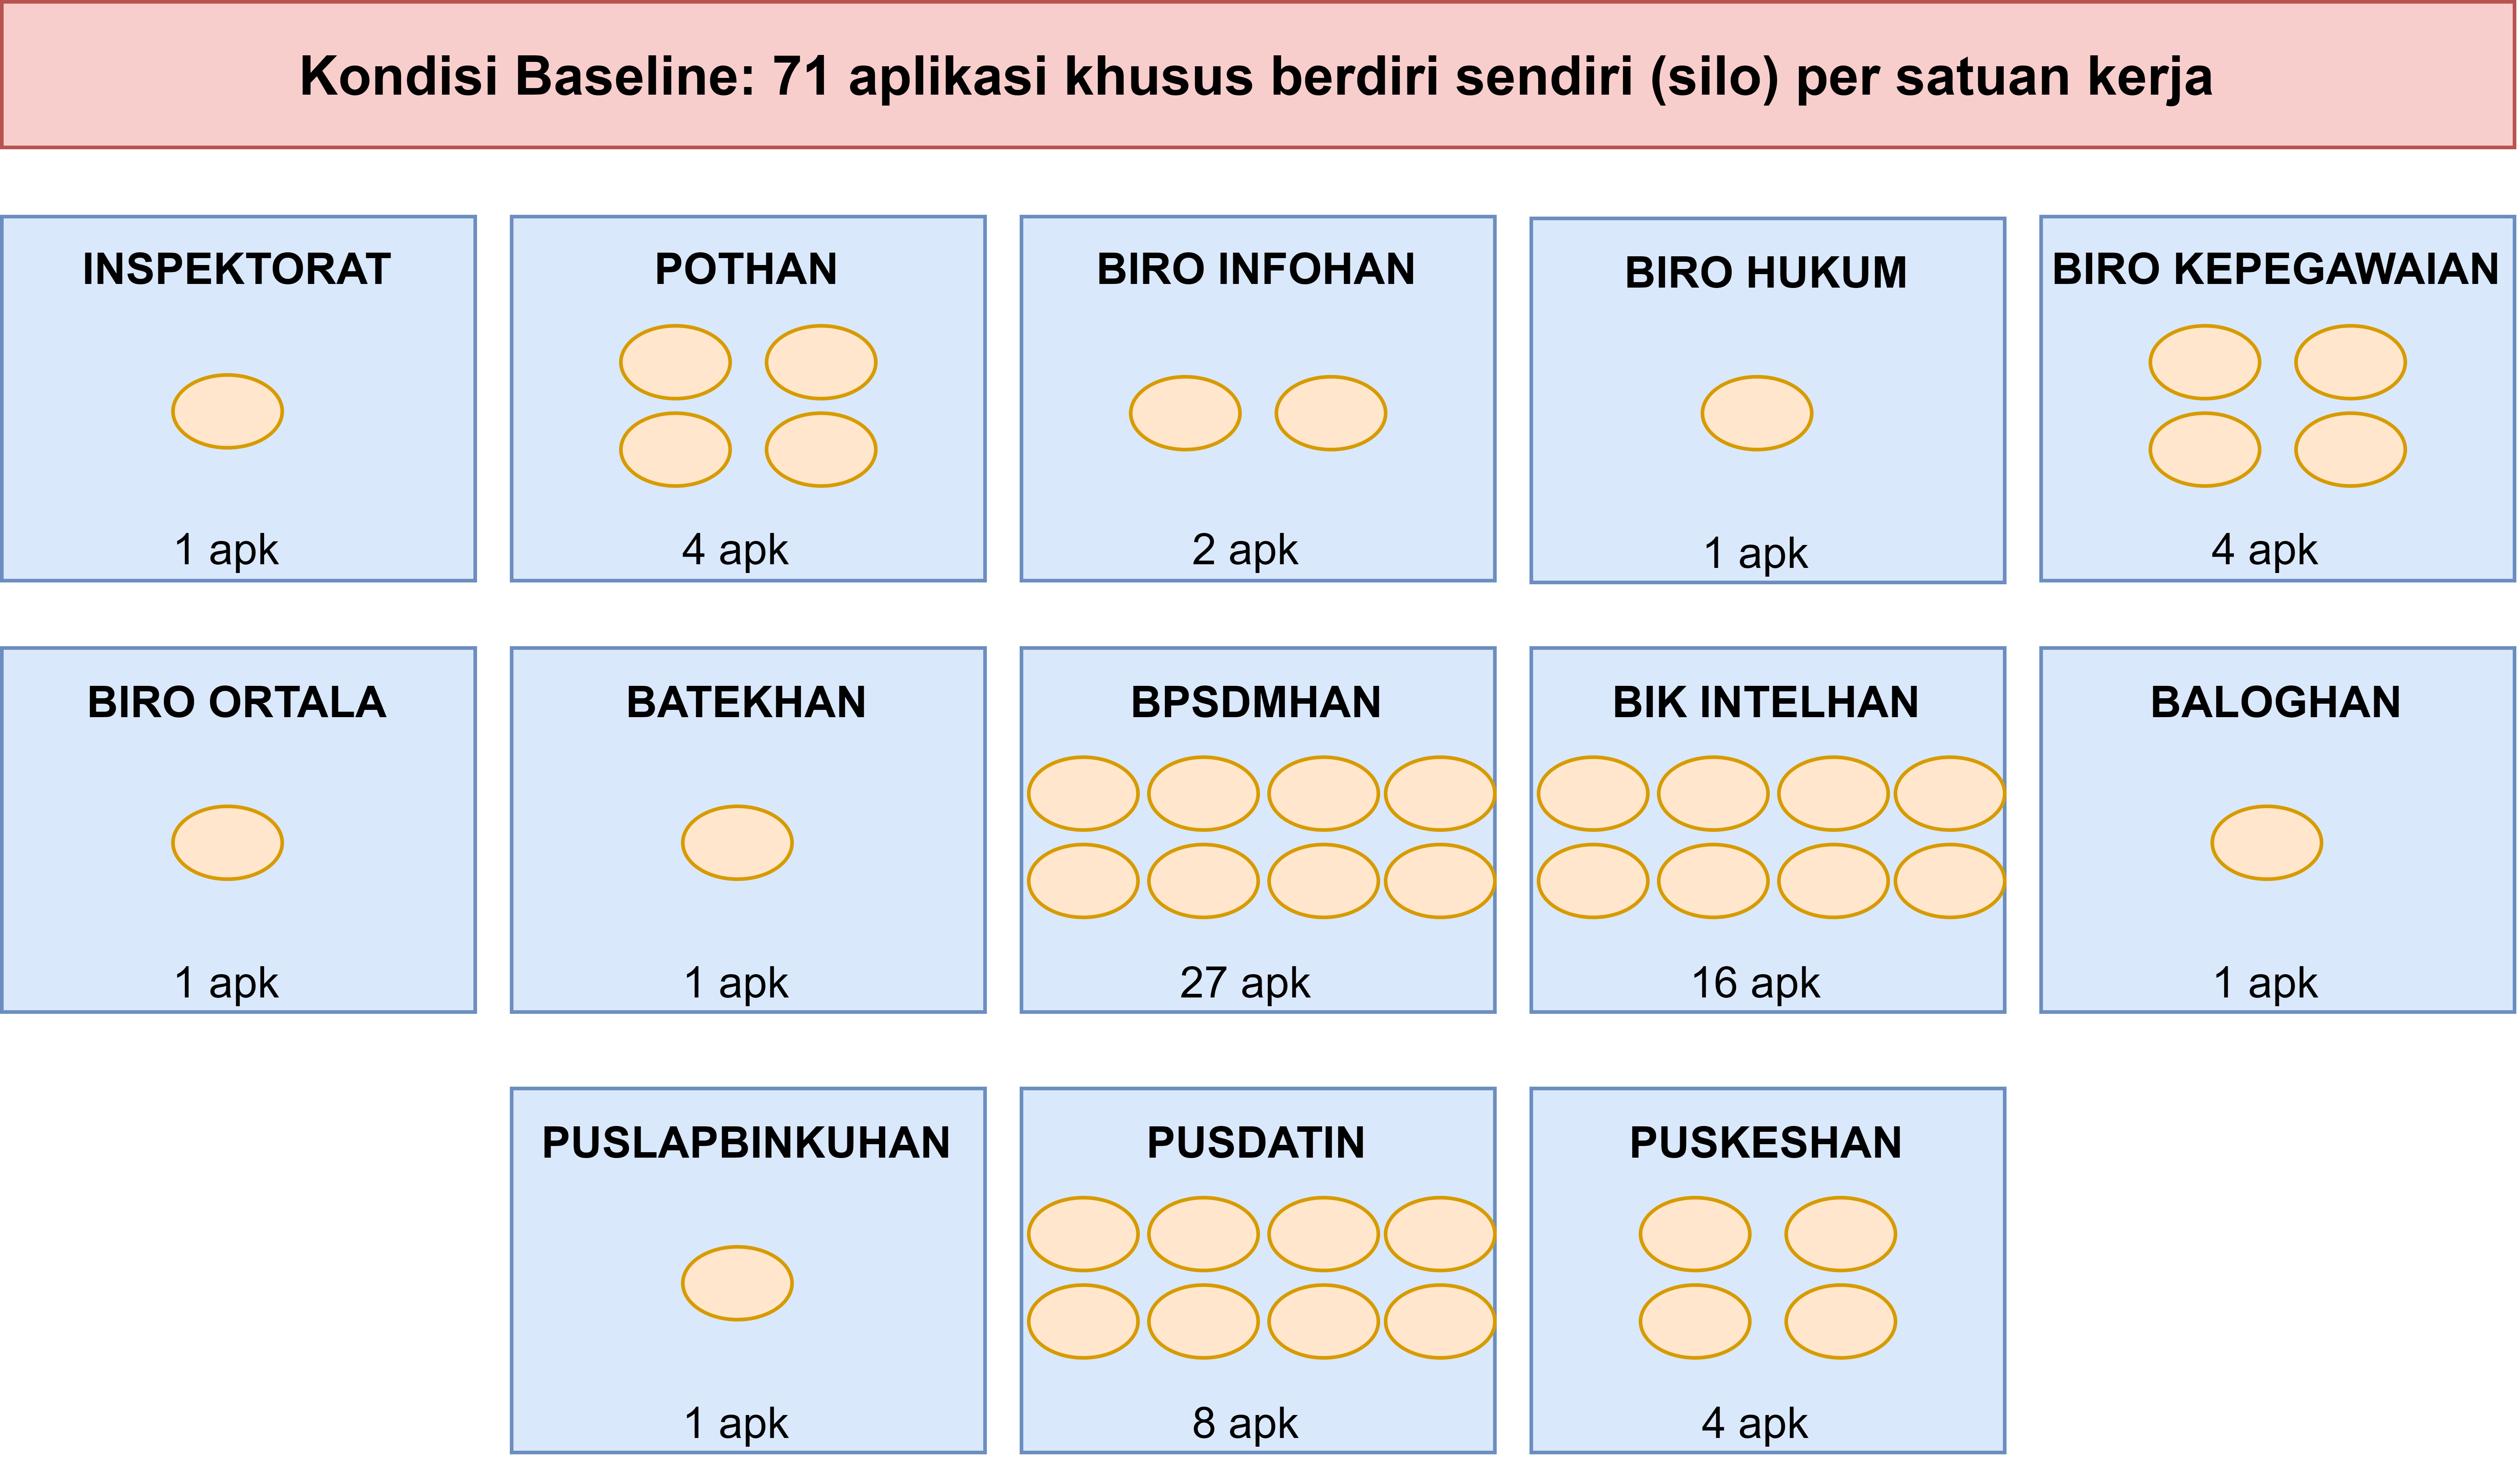
\includegraphics[width=0.99\linewidth,height=0.8\textheight,keepaspectratio]{images/Baseline Integrasi antar Aplikasi (Silo).drawio.png}
\caption{Aplikasi \textit{Baseline}}
\label{fig:IV.10}
\end{figure}

Gambar~\ref{fig:IV.10} menunjukkan bahwa pertukaran data antaraplikasi masih dilakukan secara manual atau terbatas. Kondisi ini menimbulkan tiga persoalan, yaitu duplikasi pemasukan data, akun terpisah untuk setiap aplikasi, dan sulitnya menyajikan data terpadu bagi pimpinan.

\subsubsection{Rasionalisasi Aplikasi}
\label{sec:IV.4.2.3}

Rasionalisasi menentukan tindak lanjut setiap kelompok aplikasi dengan mempertimbangkan tumpang tindih fungsi, tingkat penggunaan, dan kesesuaian dengan kapabilitas target. Hasilnya disajikan pada Tabel~\ref{tab:IV.18}.

\begingroup\small\setstretch{1.0}
\begin{longtable}{@{}>{\raggedright\arraybackslash\hspace{0pt}}p{0.246\linewidth}>{\raggedright\arraybackslash\hspace{0pt}}p{0.104\linewidth}>{\raggedright\arraybackslash\hspace{0pt}}p{0.194\linewidth}>{\raggedright\arraybackslash\hspace{0pt}}p{0.363\linewidth}@{}}
\caption{Rasionalisasi Aplikasi}\label{tab:IV.18}\\
\toprule
\textbf{Kelompok Aplikasi} & \textbf{Jumlah} & \textbf{Keputusan} & \textbf{Alasan}\\
\midrule
\endfirsthead
\multicolumn{4}{@{}l}{\small\itshape \tablename\ \thetable{} (lanjutan)}\\
\toprule
\textbf{Kelompok Aplikasi} & \textbf{Jumlah} & \textbf{Keputusan} & \textbf{Alasan}\\
\midrule
\endhead
\bottomrule
\endlastfoot
Kepegawaian & \centering\arraybackslash 4 & Digabungkan & Fungsi serupa disatukan menjadi layanan kepegawaian terpadu\\
Hukum dan Pengawasan & \centering\arraybackslash 2 & Dipertahankan + integrasi & Fungsi khas; dihubungkan ke platform integrasi\\
Informasi Publik & \centering\arraybackslash 2 & Dipertahankan + integrasi & Fungsi khas; dihubungkan ke platform integrasi\\
Potensi Pertahanan & \centering\arraybackslash 4 & Dipertahankan + integrasi & Fungsi khas; dihubungkan ke platform integrasi\\
Sarana Pertahanan & \centering\arraybackslash 1 & Dipertahankan + integrasi & Fungsi khas; dihubungkan ke platform integrasi\\
Pendidikan dan Pelatihan & \centering\arraybackslash 27 & Digabungkan & Modul bahan ajar dan VR yang terpisah disatukan ke platform pembelajaran (LMS) terpadu\\
Kesehatan dan Rehabilitasi & \centering\arraybackslash 4 & Dipertahankan + integrasi & Fungsi khas; dihubungkan ke platform integrasi\\
Data Strategis dan Geospasial & \centering\arraybackslash 8 & Dipertahankan + integrasi & Menjadi sumber utama Portal Satu Data Pertahanan\\
Keamanan Siber dan Infrastruktur TIK & \centering\arraybackslash 16 & Dipertahankan + integrasi & Fungsi teknis berbeda; pemantauannya dipadukan melalui SIEM/SOC terpadu\\
Litbang dan Keuangan & \centering\arraybackslash 2 & Dipertahankan + integrasi & Fungsi khas; dihubungkan ke platform integrasi\\
\end{longtable}
\endgroup

Tabel~\ref{tab:IV.18} menunjukkan bahwa 31 aplikasi pada kelompok kepegawaian serta pendidikan dan pelatihan digabungkan menjadi dua layanan terpadu, sedangkan 40 aplikasi lainnya dipertahankan dan dihubungkan ke platform integrasi. Aplikasi persuratan dan penyimpanan dokumen dipertahankan karena melayani satuan kerja yang berbeda, tetapi datanya dibagipakaikan melalui platform integrasi.

\subsubsection{Arsitektur Aplikasi Target}
\label{sec:IV.4.2.4}

Arsitektur aplikasi target terdiri atas aplikasi hasil rasionalisasi dan komponen baru yang menutup kesenjangan kapabilitas, yaitu:
\begin{enumerate}[label=\arabic*.]
\item Platform Integrasi Pertahanan, yang menyediakan API Gateway dan pertukaran data (\textit{data exchange}) antaraplikasi serta menaungi Portal Satu Data Pertahanan;
\item Layanan otentikasi tunggal dan manajemen identitas (SSO/IAM) tingkat \textit{enterprise}, yang memperluas SSO yang telah ada ke seluruh aplikasi;
\item Layanan kepegawaian terpadu dan platform pembelajaran (\textit{Learning Management System}, LMS) terpadu sebagai hasil penggabungan aplikasi; dan
\item Portal layanan terpadu bagi pengguna internal dan publik.
\end{enumerate}

\subsubsection{Interoperabilitas dan Integrasi Antar Aplikasi Target}
\label{sec:IV.4.2.5}

Pada kondisi target, aplikasi terhubung melalui Platform Integrasi Pertahanan dengan Portal Satu Data Pertahanan sebagai simpulnya, sebagaimana ditunjukkan pada Gambar~\ref{fig:IV.11}.
\begin{figure}[htbp]
\centering
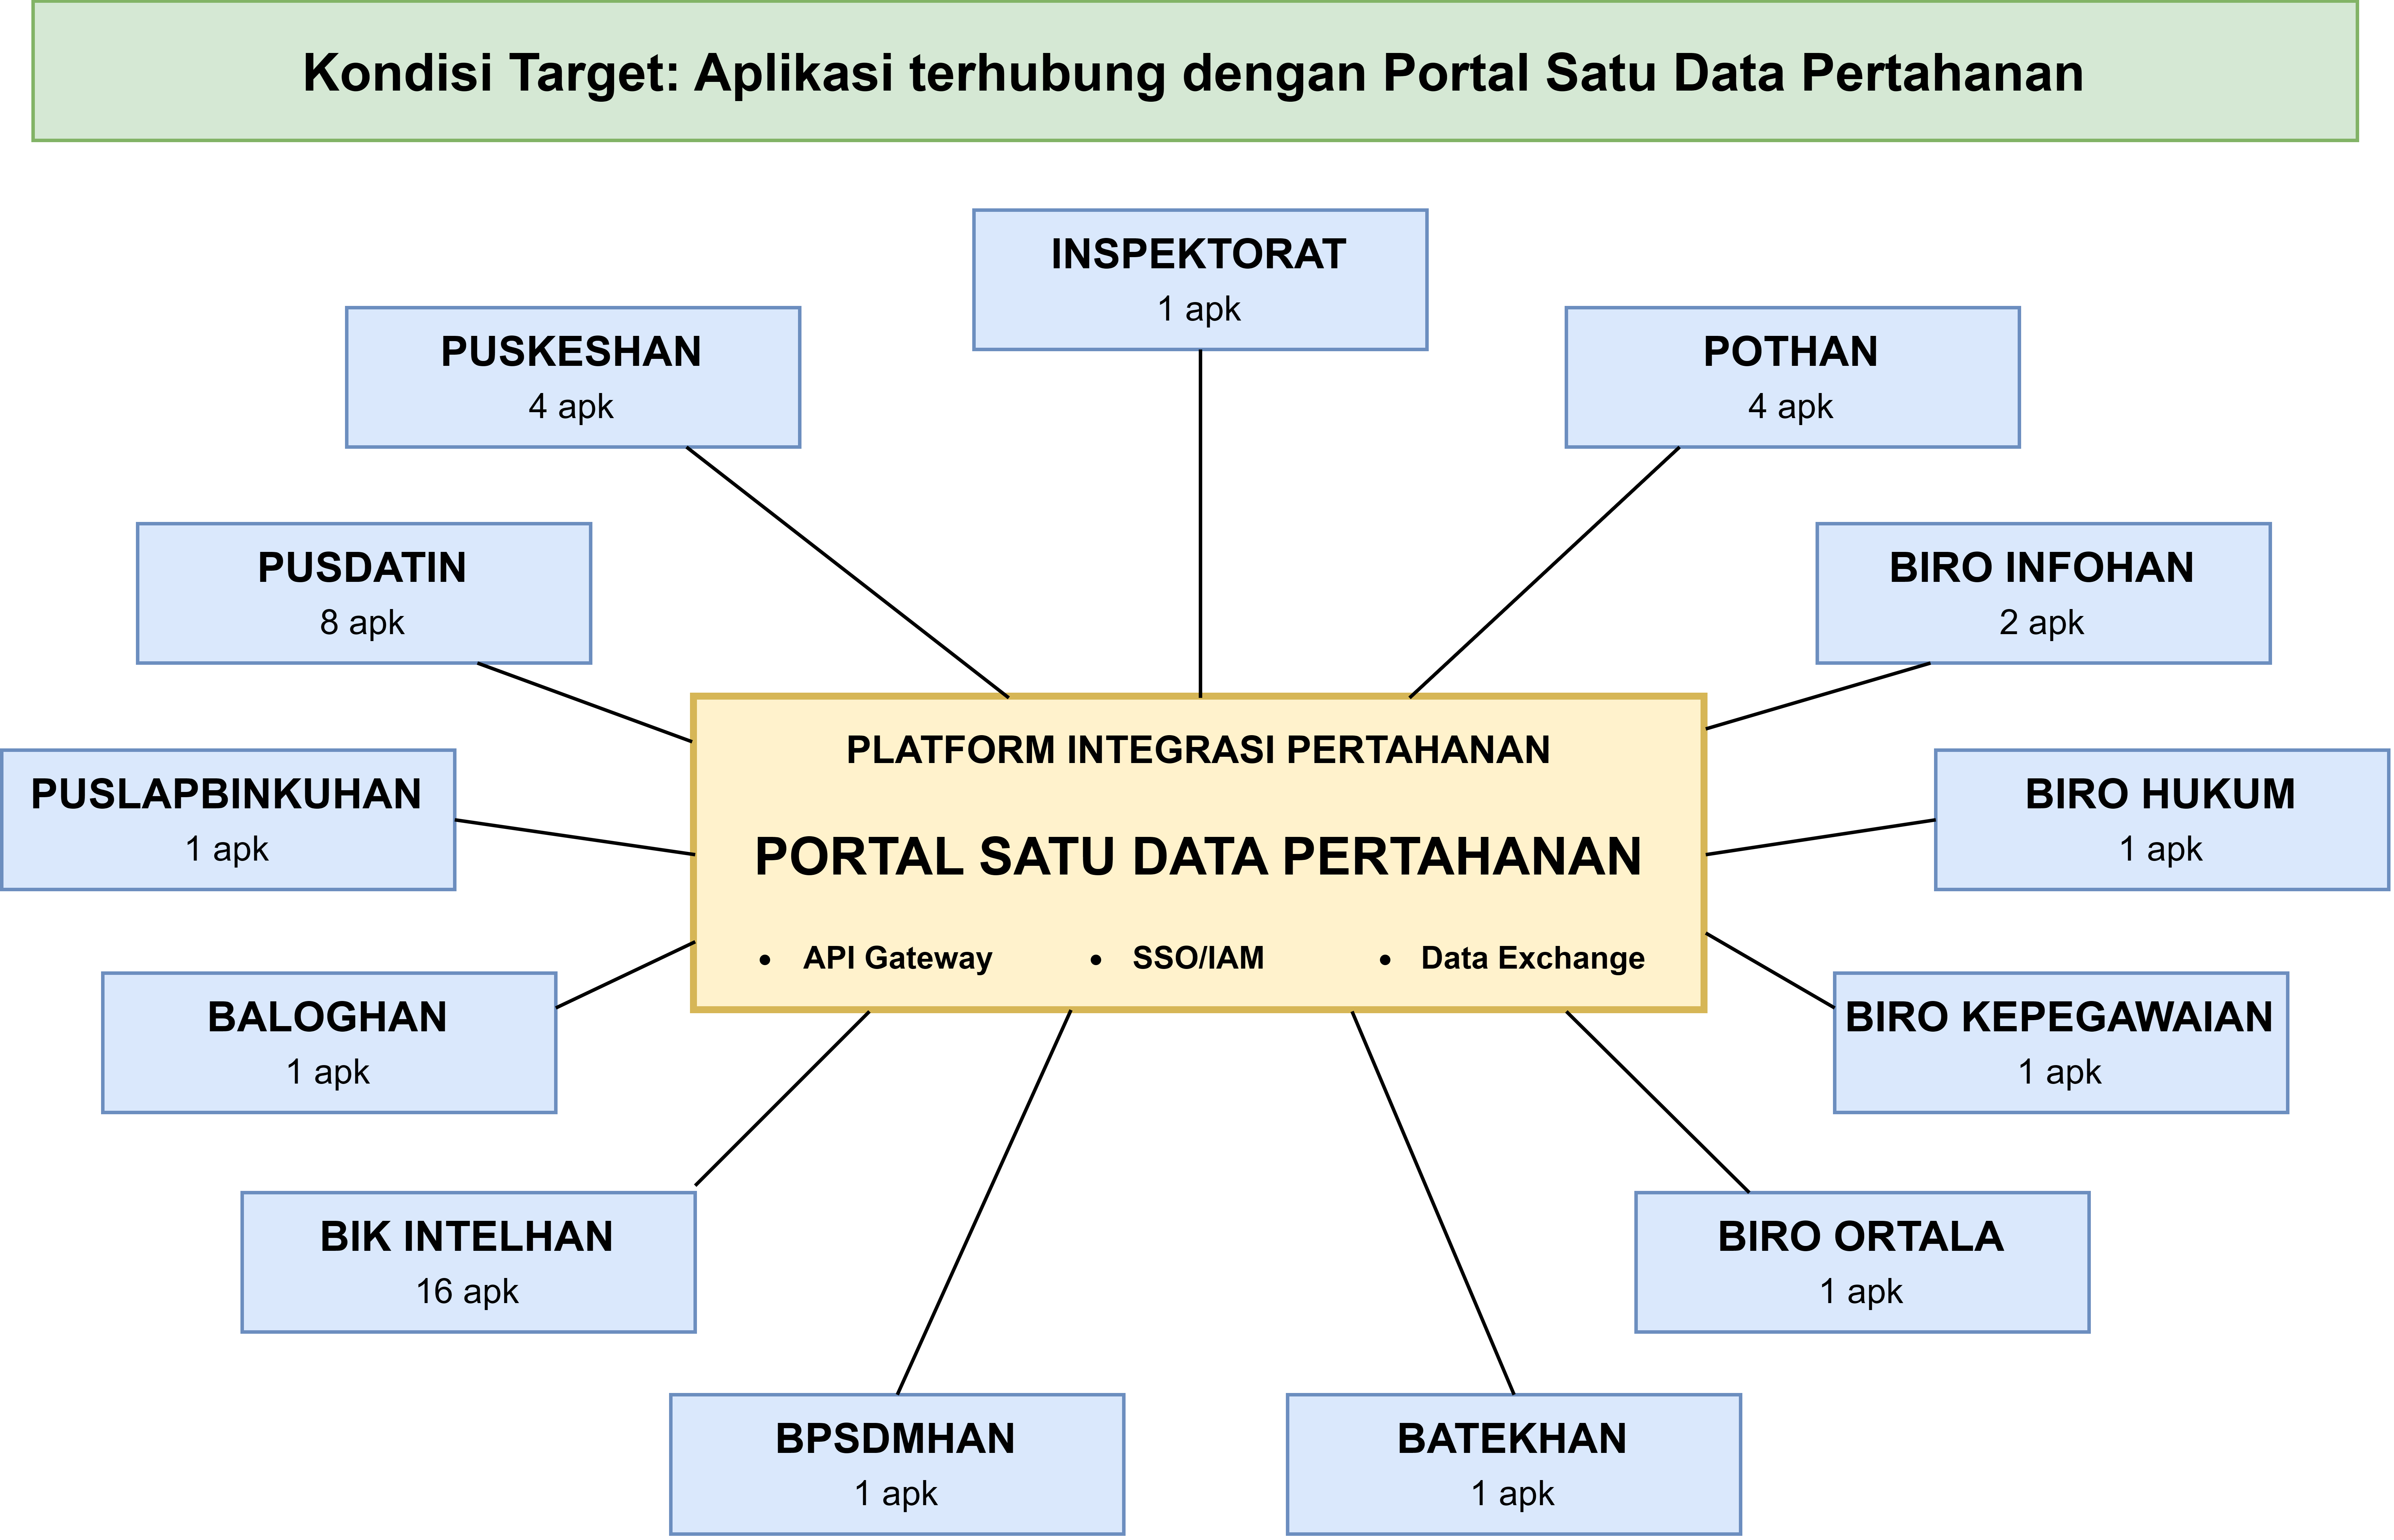
\includegraphics[width=0.99\linewidth,height=0.8\textheight,keepaspectratio]{images/Model Integrasi Target dengan Rasionalisasi Aplikasi.drawio.png}
\caption{Model Integrasi Aplikasi Target}
\label{fig:IV.11}
\end{figure}

Gambar~\ref{fig:IV.11} menunjukkan model \textit{hub} yang menggantikan pola \textit{silo} pada Gambar~\ref{fig:IV.10}. Pertukaran data dilakukan melalui API Gateway dan \textit{data exchange} dengan otentikasi tunggal (SSO/IAM), serta dikendalikan sesuai klasifikasi data pada Tabel~\ref{tab:IV.14}. Setiap aplikasi cukup terhubung ke satu platform, sehingga integrasi menjadi lebih sederhana, aman, dan mudah dikelola.

\subsubsection{Analisis Kesenjangan Aplikasi}
\label{sec:IV.4.2.6}

Analisis kesenjangan arsitektur aplikasi disajikan pada Tabel~\ref{tab:IV.19}.

\begingroup\small\setstretch{1.0}
\begin{longtable}{@{}>{\raggedright\arraybackslash\hspace{0pt}}p{0.063\linewidth}>{\raggedright\arraybackslash\hspace{0pt}}p{0.157\linewidth}>{\raggedright\arraybackslash\hspace{0pt}}p{0.219\linewidth}>{\raggedright\arraybackslash\hspace{0pt}}p{0.219\linewidth}>{\raggedright\arraybackslash\hspace{0pt}}p{0.219\linewidth}@{}}
\caption{Analisis Kesenjangan Arsitektur Aplikasi}\label{tab:IV.19}\\
\toprule
\textbf{No.} & \textbf{Aspek} & \textbf{Kondisi \textit{Baseline}} & \textbf{Kondisi Target} & \textbf{Tindak Lanjut}\\
\midrule
\endfirsthead
\multicolumn{5}{@{}l}{\small\itshape \tablename\ \thetable{} (lanjutan)}\\
\toprule
\textbf{No.} & \textbf{Aspek} & \textbf{Kondisi \textit{Baseline}} & \textbf{Kondisi Target} & \textbf{Tindak Lanjut}\\
\midrule
\endhead
\bottomrule
\endlastfoot
\centering\arraybackslash 1 & Integrasi antaraplikasi & Aplikasi \textit{silo}; pertukaran data manual & Aplikasi terhubung melalui platform integrasi & Pembangunan platform integrasi dan API Gateway\\
\centering\arraybackslash 2 & Redundansi fungsi & Aplikasi berfungsi serupa pada kepegawaian dan pembelajaran & Portofolio ramping dan terkonsolidasi & Penggabungan menjadi layanan kepegawaian dan LMS terpadu\\
\centering\arraybackslash 3 & Otentikasi dan akses & Akun terpisah per aplikasi; SSO belum mencakup seluruh aplikasi & SSO/IAM tingkat \textit{enterprise} & Perluasan SSO/IAM ke seluruh aplikasi\\
\centering\arraybackslash 4 & Dukungan kapabilitas & Integrasi data dan komando-kendali lintas matra belum didukung aplikasi & Komponen baru sesuai kapabilitas target & Pengembangan komponen baru; komando-kendali dirinci pada Fase \textit{C6ISR Architecture}\\
\centering\arraybackslash 5 & Tata kelola aplikasi & Pengelolaan aplikasi tersebar per satuan kerja & Tata kelola portofolio aplikasi terpusat & Penetapan tata kelola portofolio aplikasi oleh DTO\\
\end{longtable}
\endgroup

Tabel~\ref{tab:IV.19} menunjukkan bahwa platform integrasi menjadi prasyarat bagi penutupan kesenjangan lainnya.

\subsubsection{\textit{Roadmap} Implementasi}
\label{sec:IV.4.3}

\textit{Roadmap} Fase \textit{Information Systems Architecture} menyusun inisiatif data dan aplikasi untuk menutup kesenjangan pada Tabel~\ref{tab:IV.16} dan Tabel~\ref{tab:IV.19} dalam tiga horizon waktu, sebagaimana disajikan pada Gambar~\ref{fig:IV.12}.
\begin{figure}[htbp]
\centering
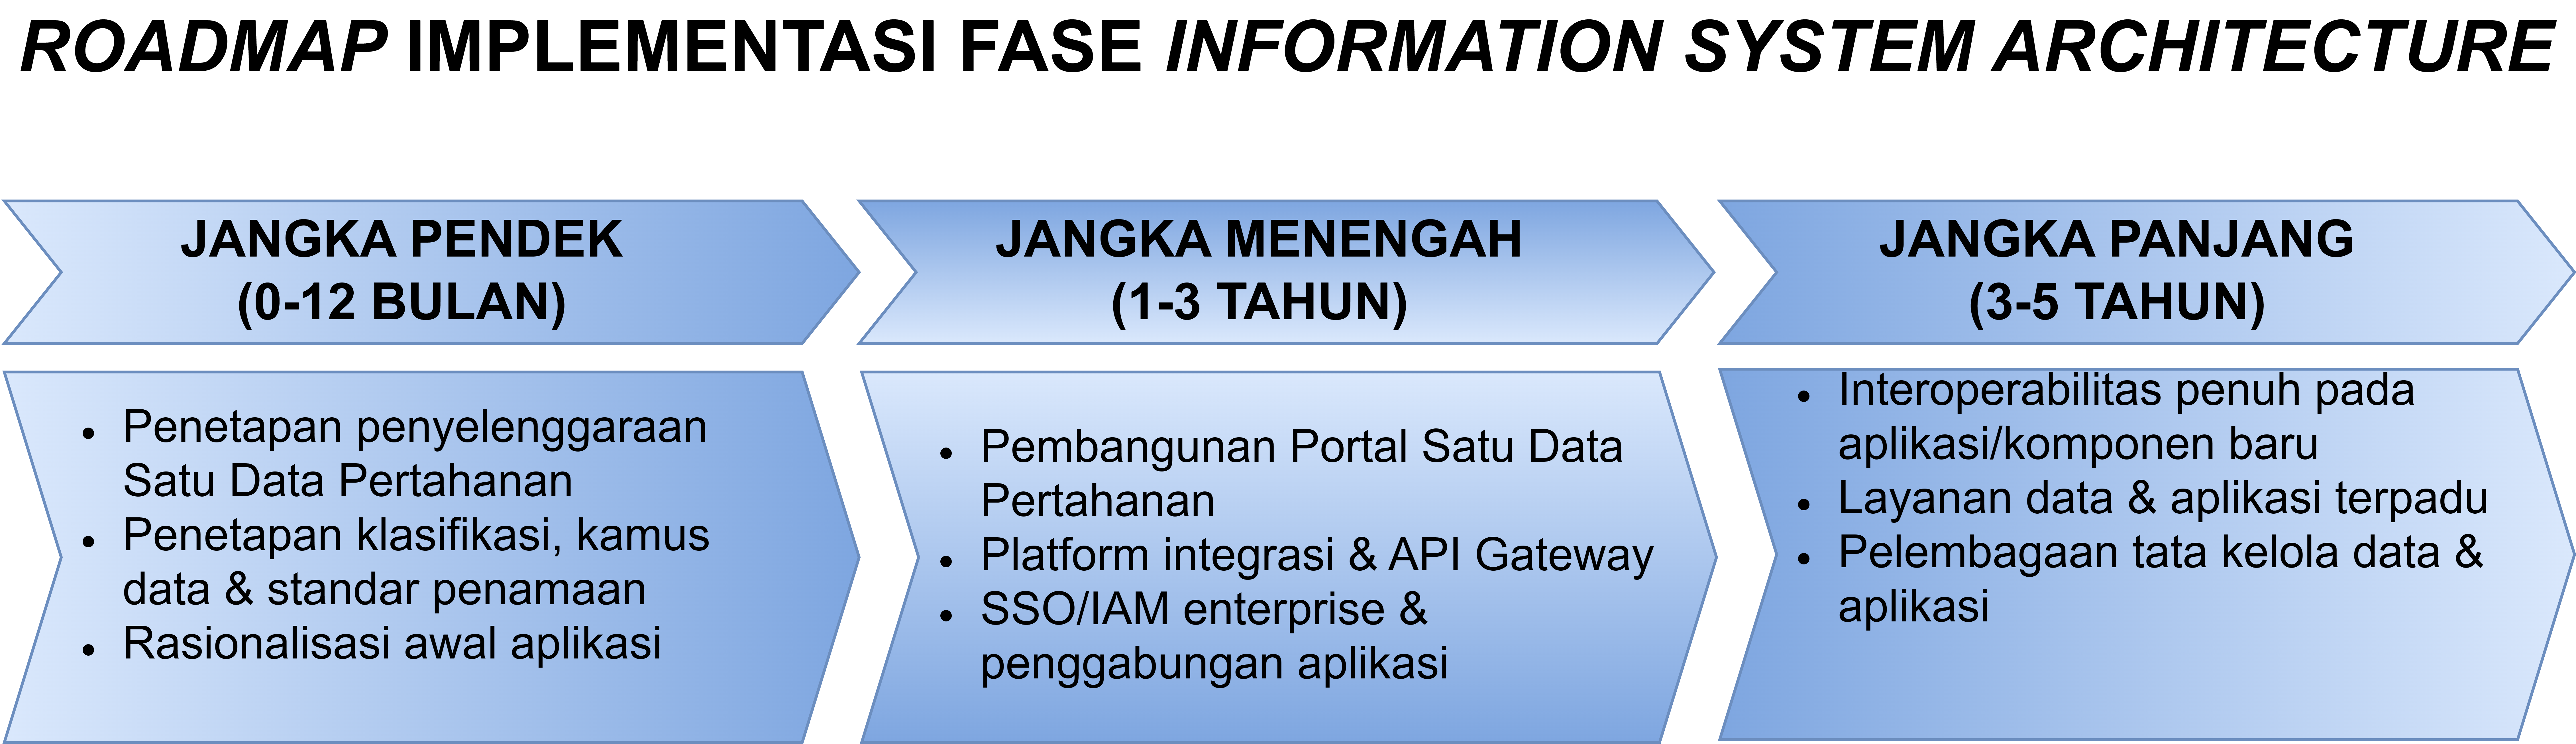
\includegraphics[width=0.99\linewidth,height=0.8\textheight,keepaspectratio]{images/Roadmap implementasi fase Information System Architecture.drawio.png}
\caption{\textit{Roadmap} Implementasi Fase \textit{Information Systems Architecture}}
\label{fig:IV.12}
\end{figure}

Gambar~\ref{fig:IV.12} menunjukkan bahwa jangka pendek (0–12 bulan) difokuskan pada inisiatif nonteknis, yaitu penetapan penyelenggara Satu Data Pertahanan, klasifikasi, kamus data, dan standar penamaan, serta rasionalisasi awal aplikasi. Jangka menengah (1–3 tahun) membangun Portal Satu Data Pertahanan, platform integrasi dan API Gateway, serta SSO/IAM \textit{enterprise}, sekaligus menggabungkan aplikasi berfungsi serupa. Jangka panjang (3–5 tahun) diarahkan pada interoperabilitas penuh, termasuk dengan Portal Satu Data Indonesia, layanan data dan aplikasi terpadu, serta kelembagaan tata kelola data dan aplikasi.

Dengan demikian, Fase Information Systems Architecture menghasilkan arsitektur data dan aplikasi target yang menjadi dasar perancangan infrastruktur pada Fase Technology Architecture.

\section{Fase Technology Architecture}
\label{sec:IV.5}

Fase Technology Architecture merancang infrastruktur teknologi yang menopang arsitektur data dan aplikasi. Perancangan berpedoman pada prinsip arsitektur pada Tabel~\ref{tab:IV.1} serta mengacu pada Permenhan Nomor 34 Tahun 2025 tentang Peta Jalan Pelindungan Infrastruktur Informasi Vital Sektor Pertahanan \cite{Permenhan34Tahun2025} untuk aspek keamanan.

\subsection{Arsitektur Teknologi \textit{Baseline}}
\label{sec:IV.5.1}

Topologi jaringan dan infrastruktur pusat data Kemhan secara rinci tidak tersedia dalam penelitian ini. Oleh karena itu, arsitektur teknologi \textit{baseline} disusun sebagai model logis berdasarkan informasi yang tersedia, sebagaimana disajikan pada Gambar~\ref{fig:IV.13}.
\begin{figure}[htbp]
\centering
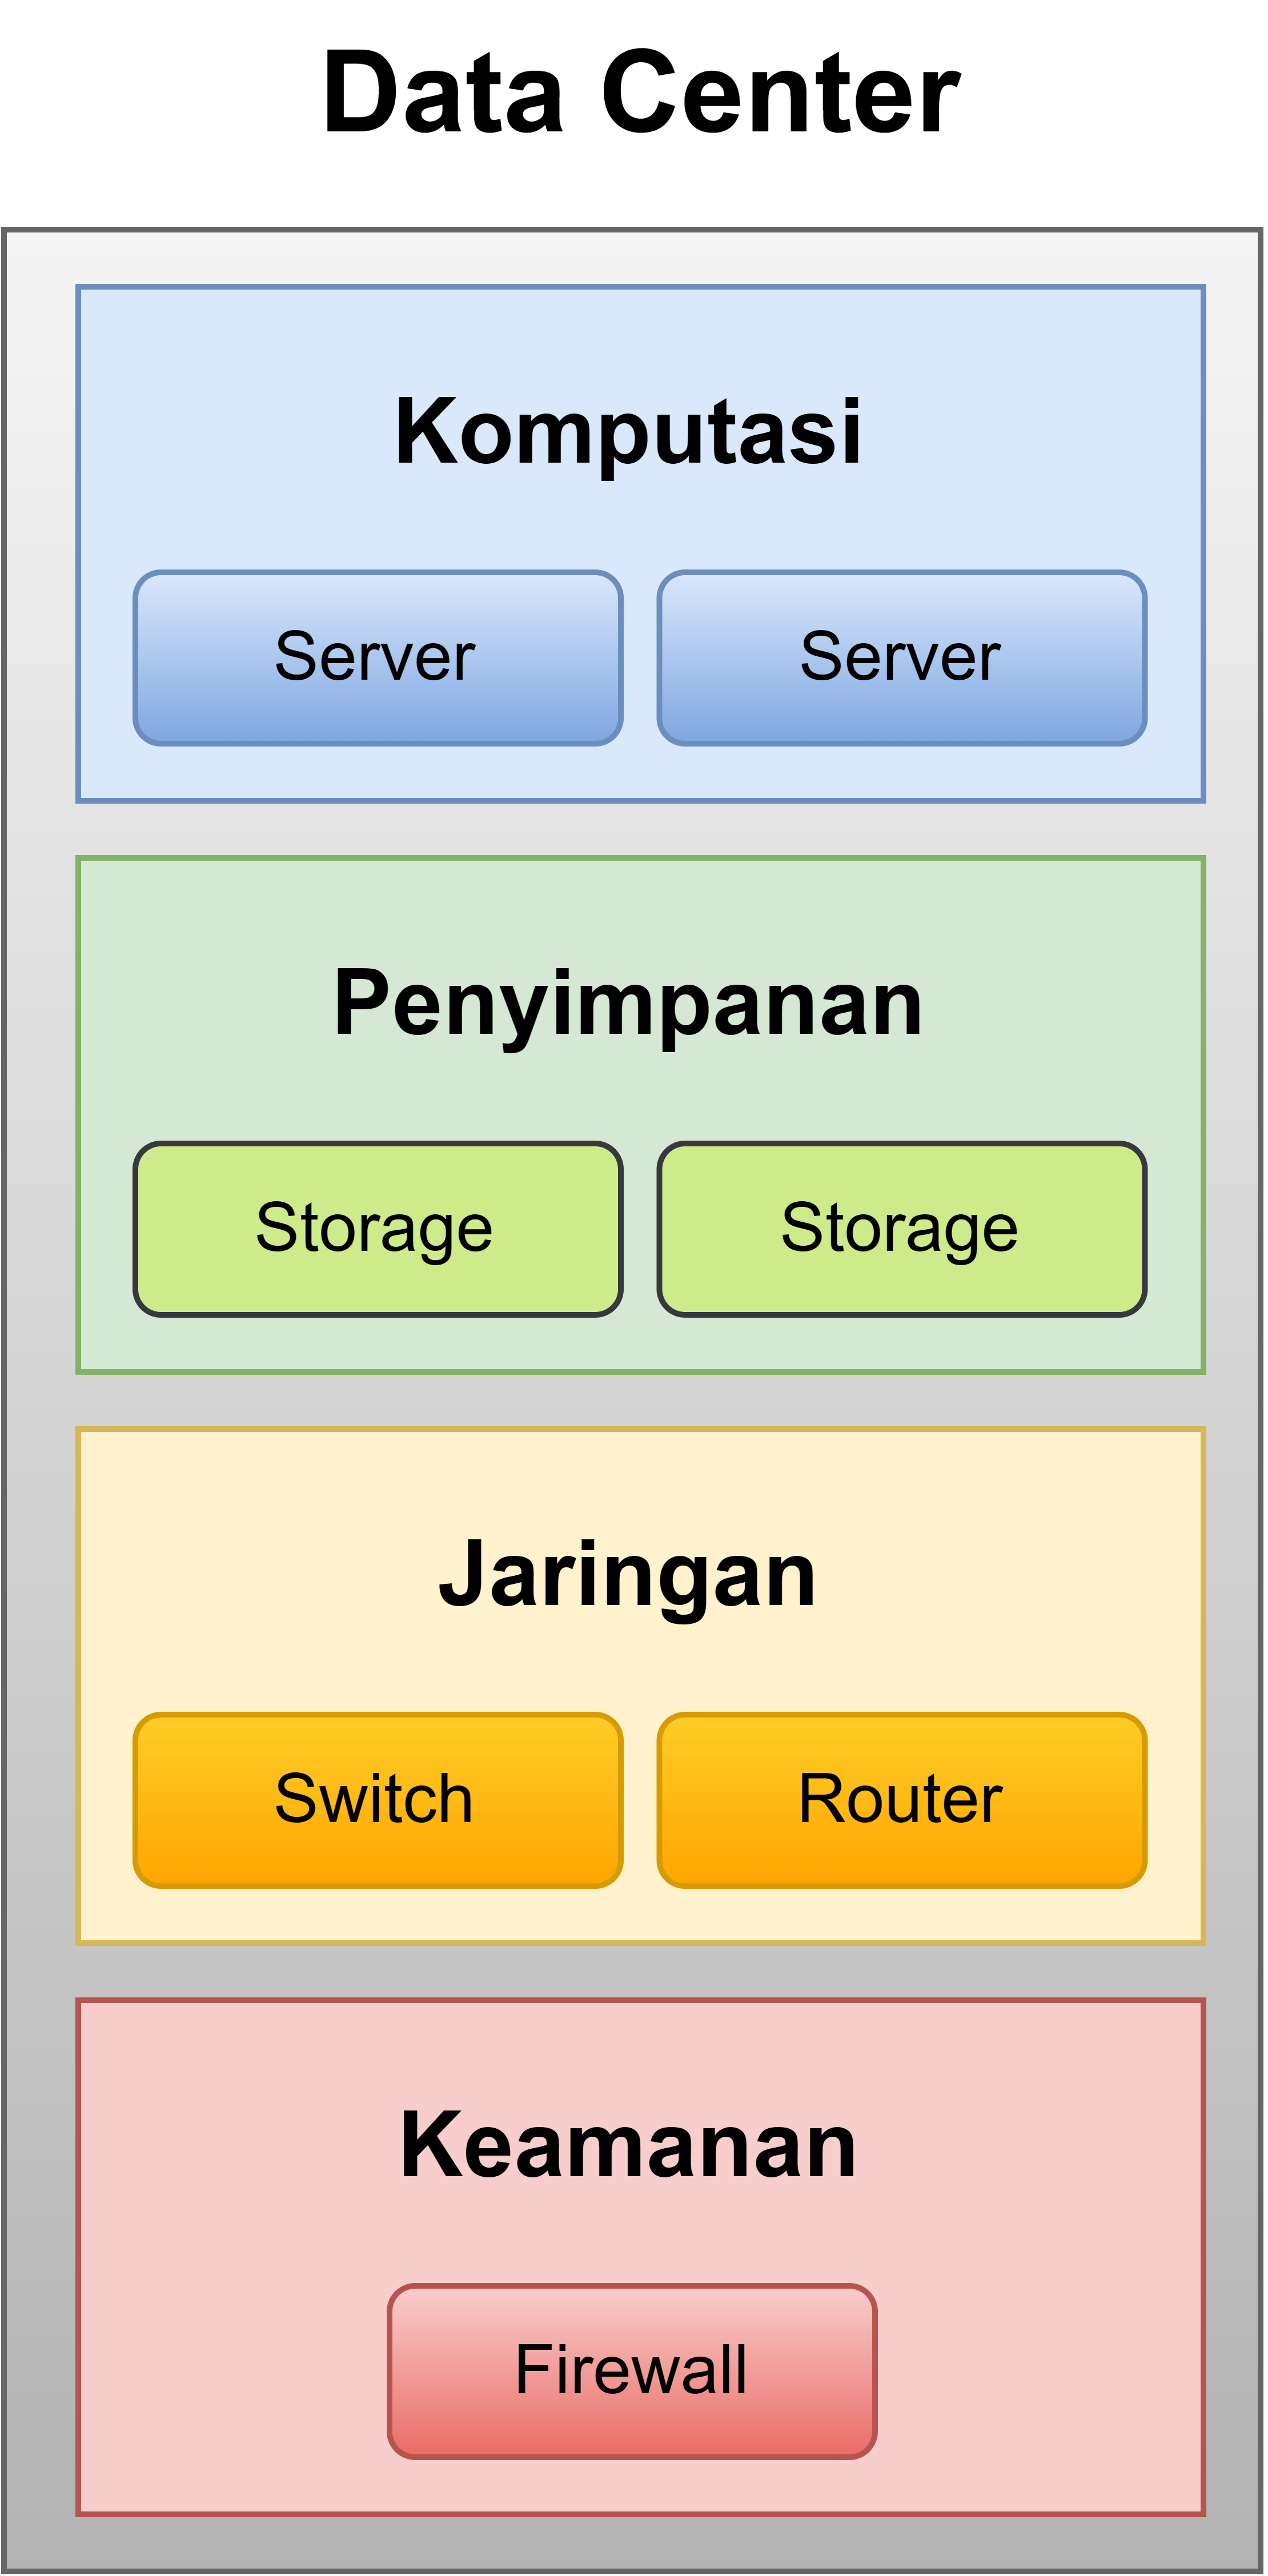
\includegraphics[width=0.33\linewidth,height=0.8\textheight,keepaspectratio]{images/Arsitektur Teknologi Baseline.drawio.png}
\caption{Arsitektur Teknologi \textit{Baseline}}
\label{fig:IV.13}
\end{figure}

Gambar~\ref{fig:IV.13} menunjukkan bahwa infrastruktur teknologi Kemhan berpusat pada satu \textit{Data Center} di Pusat Data dan Informasi, Pondok Labu, Jakarta Selatan. Infrastruktur tersebut tersusun atas empat lapisan, yaitu komputasi (server), penyimpanan (\textit{storage}), jaringan (\textit{switch} dan \textit{router}), serta keamanan (\textit{firewall}).

Dari kondisi tersebut teridentifikasi dua karakteristik utama. Pertama, seluruh layanan bertumpu pada satu \textit{Data Center} tanpa \textit{Disaster Recovery Center} (DRC) maupun redundansi, sehingga menjadi titik tunggal kegagalan (\textit{single point of failure}). Kedua, lapisan keamanan masih bersifat parsial dan belum diterapkan secara menyeluruh.

\subsection{Prinsip dan Standar Teknologi}
\label{sec:IV.5.2}

Penerapan prinsip arsitektur pada domain teknologi disajikan pada Tabel~\ref{tab:IV.20}.

\begingroup\small\setstretch{1.0}
\begin{longtable}{@{}>{\raggedright\arraybackslash\hspace{0pt}}p{0.311\linewidth}>{\raggedright\arraybackslash\hspace{0pt}}p{0.656\linewidth}@{}}
\caption{Prinsip dan Standar Teknologi}\label{tab:IV.20}\\
\toprule
\textbf{Prinsip} & \textbf{Penerapan pada Arsitektur Teknologi}\\
\midrule
\endfirsthead
\multicolumn{2}{@{}l}{\small\itshape \tablename\ \thetable{} (lanjutan)}\\
\toprule
\textbf{Prinsip} & \textbf{Penerapan pada Arsitektur Teknologi}\\
\midrule
\endhead
\bottomrule
\endlastfoot
\textit{Availability \& Reliability} & \textit{Data Center} dilengkapi DRC, redundansi, dan cadangan (\textit{backup}) untuk menjamin ketersediaan layanan\\
\textit{Security by Design} & Keamanan diterapkan sejak perancangan pada setiap lapisan sesuai Permenhan Nomor 34 Tahun 2025\\
\textit{Scalability \& Flexibility} & Virtualisasi dan kontainer (\textit{container}) agar sumber daya elastis dan mudah diskalakan\\
\textit{Interoperability} & Standar terbuka (\textit{open standard}) dan API untuk pertukaran data antarsistem\\
\textit{Integrated Command \& Control} & Jaringan lintas matra untuk mendukung komando dan kendali terpadu\\
\textit{Data as Strategic Asset} & Penyimpanan redundan dan cadangan terpusat untuk melindungi Data Pertahanan\\
\end{longtable}
\endgroup

Tabel~\ref{tab:IV.20} menunjukkan bahwa enam dari sembilan prinsip arsitektur diterapkan langsung pada domain teknologi. Dengan demikian, infrastruktur tidak hanya dirancang untuk ketersediaan layanan, tetapi juga untuk melindungi data dan menopang komando-kendali lintas matra.

\subsection{Arsitektur Teknologi Target}
\label{sec:IV.5.3}

Arsitektur teknologi target dirancang untuk menutup kesenjangan \textit{baseline} serta menopang Platform Integrasi Pertahanan dan Portal Satu Data Pertahanan. Arsitektur ini disusun berlapis di atas dua pusat data yang redundan, sebagaimana disajikan pada Gambar~\ref{fig:IV.14}.
\begin{figure}[htbp]
\centering
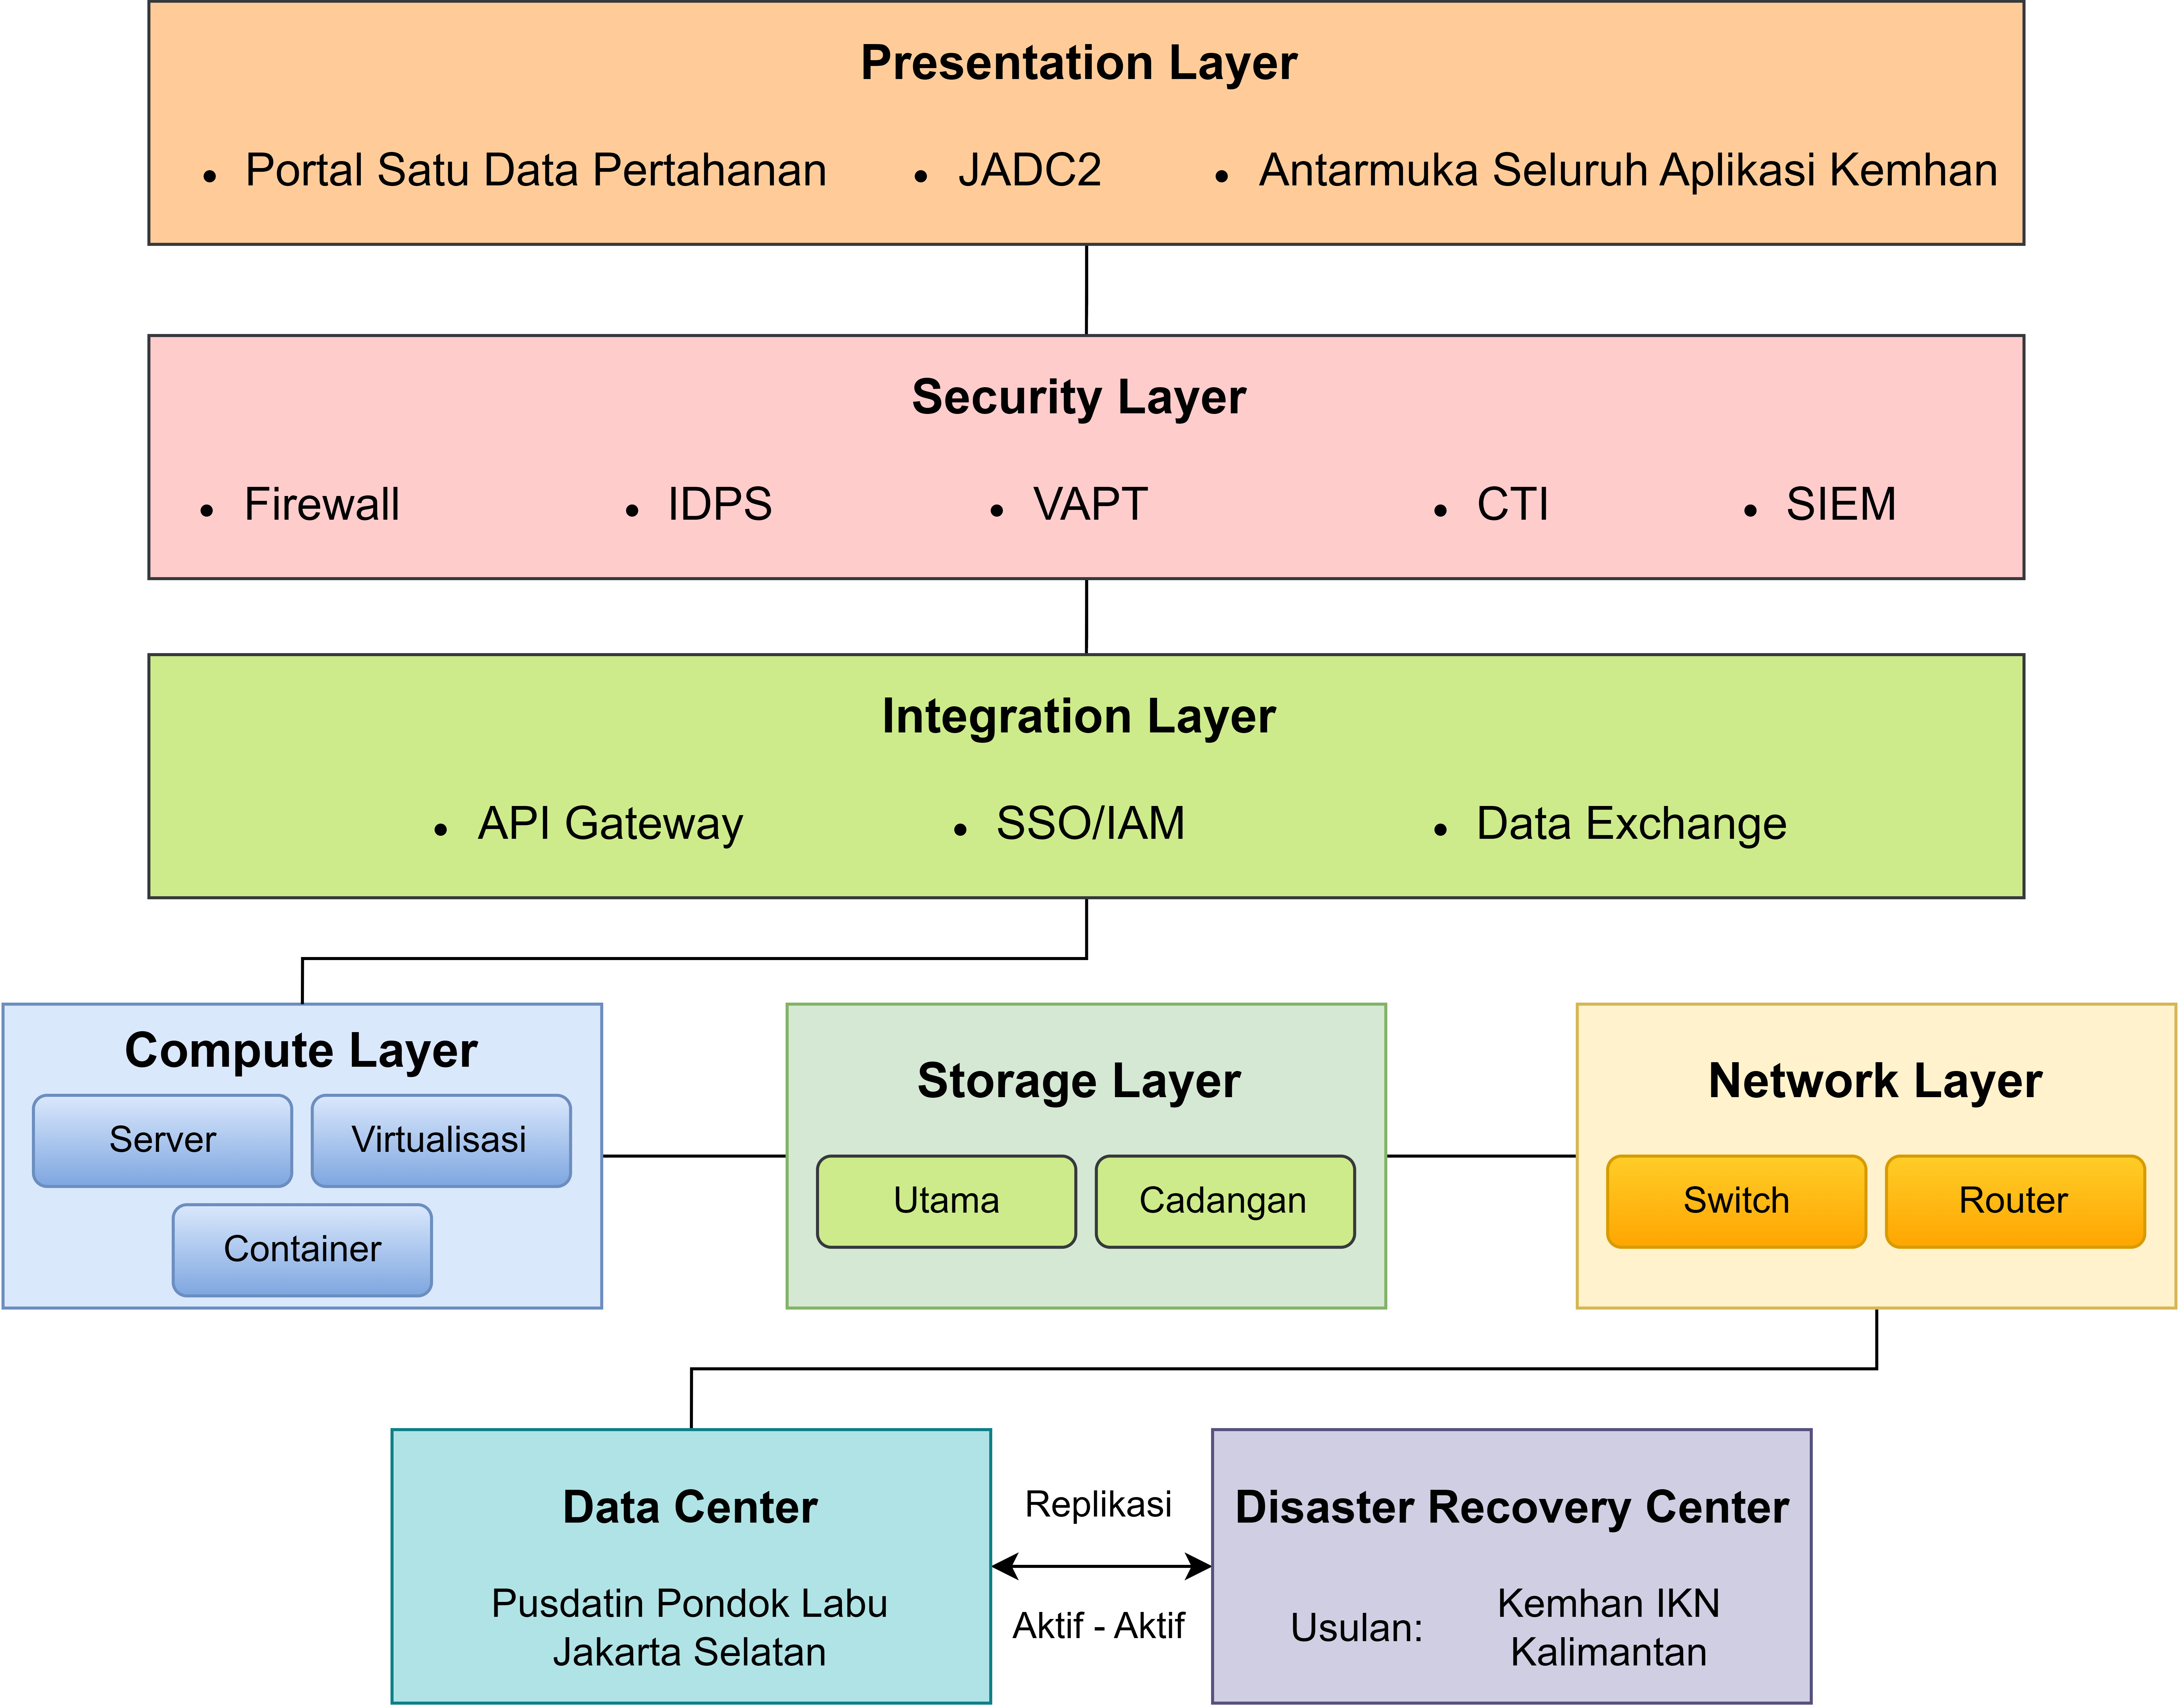
\includegraphics[width=0.99\linewidth,height=0.8\textheight,keepaspectratio]{images/Arsitektur Teknologi Target.drawio.png}
\caption{Arsitektur Teknologi Target}
\label{fig:IV.14}
\end{figure}

Gambar~\ref{fig:IV.14} menunjukkan enam lapisan dengan fungsi sebagai berikut:
\begin{enumerate}[label=\arabic*.]
\item \textit{Presentation Layer}, yaitu antarmuka pengguna yang mencakup Portal Satu Data Pertahanan, antarmuka seluruh aplikasi Kemhan, dan titik akses komando dan kendali lintas domain berbasis konsep JADC2 yang dirinci pada Fase \textit{C6ISR Architecture};
\item \textit{Security Layer}, yaitu lapisan keamanan menyeluruh yang mencakup \textit{firewall}, IDPS, VAPT, \textit{Cyber Threat Intelligence} (CTI), dan SIEM, yang dirinci pada Subbab~\ref{sec:IV.5.4};
\item \textit{Integration Layer}, yaitu API Gateway, SSO/IAM, dan \textit{data exchange} sebagai tulang punggung interoperabilitas antaraplikasi;
\item \textit{Compute Layer}, yaitu server, virtualisasi, dan kontainer agar sumber daya elastis dan mudah diskalakan;
\item \textit{Storage Layer}, yaitu penyimpanan utama dan cadangan untuk menjamin ketersediaan dan pelindungan data; dan
\item \textit{Network Layer}, yaitu jaringan tersegmentasi dan terenkripsi dengan konektivitas lintas matra.
\end{enumerate}

Seluruh lapisan ditopang oleh \textit{Data Center} Utama di Pusat Data dan Informasi, Pondok Labu, dan DRC yang diusulkan berlokasi di Kemhan IKN, Kalimantan. Keduanya beroperasi dalam konfigurasi aktif-aktif (\textit{active-active}) dengan replikasi data. Dengan konfigurasi ini, kedua pusat data melayani beban kerja secara bersamaan sekaligus saling menjadi cadangan, sehingga titik tunggal kegagalan dapat dihilangkan.

\subsection{Arsitektur Keamanan}
\label{sec:IV.5.4}

Lapisan keamanan mengacu pada Permenhan Nomor 34 Tahun 2025 \cite{Permenhan34Tahun2025}, yang mengelompokkan pelindungan ke dalam empat domain, yaitu identifikasi, proteksi, deteksi, serta penanggulangan dan pemulihan. Komponen keamanan pada setiap domain disajikan pada Tabel~\ref{tab:IV.21}.

\begingroup\small\setstretch{1.0}
\begin{longtable}{@{}>{\raggedright\arraybackslash\hspace{0pt}}p{0.201\linewidth}>{\raggedright\arraybackslash\hspace{0pt}}p{0.401\linewidth}>{\raggedright\arraybackslash\hspace{0pt}}p{0.335\linewidth}@{}}
\caption{Komponen Keamanan per Domain}\label{tab:IV.21}\\
\toprule
\textbf{Domain} & \textbf{Komponen/Teknologi} & \textbf{Fungsi}\\
\midrule
\endfirsthead
\multicolumn{3}{@{}l}{\small\itshape \tablename\ \thetable{} (lanjutan)}\\
\toprule
\textbf{Domain} & \textbf{Komponen/Teknologi} & \textbf{Fungsi}\\
\midrule
\endhead
\bottomrule
\endlastfoot
Identifikasi & \textit{Vulnerability Assessment and Penetration Test} (VAPT) & Mengidentifikasi kerentanan dan risiko keamanan sistem\\
Proteksi & \textit{Firewall}, segmentasi jaringan, \textit{endpoint protection}, dan \textit{Intrusion Detection and Prevention System} (IDPS) & Melindungi jaringan dan perangkat akhir serta mencegah serangan\\
Deteksi & \textit{Cyber Threat Intelligence} (CTI) dan \textit{Security Information and Event Management} (SIEM) & Mendeteksi anomali dan peristiwa keamanan siber\\
Penanggulangan dan Pemulihan & \textit{Digital forensic}, \textit{Security Orchestration, Automation and Response} (SOAR), \textit{Computer Security Incident Response Team} (CSIRT), sistem cadangan, dan DRC & Menanggulangi insiden siber serta memulihkan layanan dan sistem\\
\end{longtable}
\endgroup

Tabel~\ref{tab:IV.21} menunjukkan bahwa sebagian komponen telah tersedia pada kondisi \textit{baseline}, seperti VAPT, SIEM, dan Helpdesk CSIRT (Tabel~\ref{tab:IV.17}). Oleh karena itu, arah pengembangannya adalah memadukan komponen tersebut dalam satu pusat operasi keamanan.

Sesuai peta jalan tersebut, kematangan keamanan siber sektor pertahanan saat ini berada pada level 1 hingga level 2. Targetnya adalah level 3 (terdefinisi) pada tahun 2029, yaitu ketika penerapan keamanan siber telah formal, dilakukan secara konsisten, dan ditinjau secara berkala.

\subsection{Analisis Kesenjangan}
\label{sec:IV.5.5}

Analisis kesenjangan arsitektur teknologi disajikan pada Tabel~\ref{tab:IV.22}.

\begingroup\small\setstretch{1.0}
\begin{longtable}{@{}>{\raggedright\arraybackslash\hspace{0pt}}p{0.063\linewidth}>{\raggedright\arraybackslash\hspace{0pt}}p{0.157\linewidth}>{\raggedright\arraybackslash\hspace{0pt}}p{0.219\linewidth}>{\raggedright\arraybackslash\hspace{0pt}}p{0.219\linewidth}>{\raggedright\arraybackslash\hspace{0pt}}p{0.219\linewidth}@{}}
\caption{Analisis Kesenjangan Arsitektur Teknologi}\label{tab:IV.22}\\
\toprule
\textbf{No.} & \textbf{Aspek} & \textbf{Kondisi \textit{Baseline}} & \textbf{Kondisi Target} & \textbf{Tindak Lanjut}\\
\midrule
\endfirsthead
\multicolumn{5}{@{}l}{\small\itshape \tablename\ \thetable{} (lanjutan)}\\
\toprule
\textbf{No.} & \textbf{Aspek} & \textbf{Kondisi \textit{Baseline}} & \textbf{Kondisi Target} & \textbf{Tindak Lanjut}\\
\midrule
\endhead
\bottomrule
\endlastfoot
\centering\arraybackslash 1 & Ketersediaan & Satu \textit{Data Center} tanpa DRC (\textit{single point of failure}) & \textit{Data Center} Utama dan DRC aktif-aktif dengan replikasi & Pembangunan DRC dan replikasi aktif-aktif\\
\centering\arraybackslash 2 & Komputasi & Server fisik & Server, virtualisasi, dan kontainer & Penerapan virtualisasi dan kontainer\\
\centering\arraybackslash 3 & Penyimpanan & Penyimpanan operasional tanpa redundansi & Penyimpanan utama dan cadangan yang redundan & Penyediaan redundansi dan cadangan data\\
\centering\arraybackslash 4 & Jaringan & Belum tersegmentasi dan belum lintas matra & Tersegmentasi, terenkripsi, dan lintas matra & Penataan dan pengamanan jaringan\\
\centering\arraybackslash 5 & Integrasi & Belum ada lapisan integrasi & \textit{Integration layer} (API Gateway, SSO/IAM, dan \textit{data exchange}) & Pembangunan lapisan integrasi\\
\centering\arraybackslash 6 & Keamanan (\textit{Security}) & Parsial (kematangan level 1–2) & Menyeluruh (kematangan level 3) & Penerapan komponen keamanan per domain\\
\end{longtable}
\endgroup

Tabel~\ref{tab:IV.22} menunjukkan bahwa kesenjangan 1 merupakan risiko terbesar, karena gangguan pada satu \textit{Data Center} dapat menghentikan seluruh layanan pertahanan.

\subsection{\textit{Roadmap}}
\label{sec:IV.5.6}

\textit{Roadmap} Fase Technology Architecture menyusun inisiatif untuk menutup kesenjangan pada Tabel~\ref{tab:IV.22} dalam tiga horizon waktu, sebagaimana disajikan pada Gambar~\ref{fig:IV.15}.
\begin{figure}[htbp]
\centering
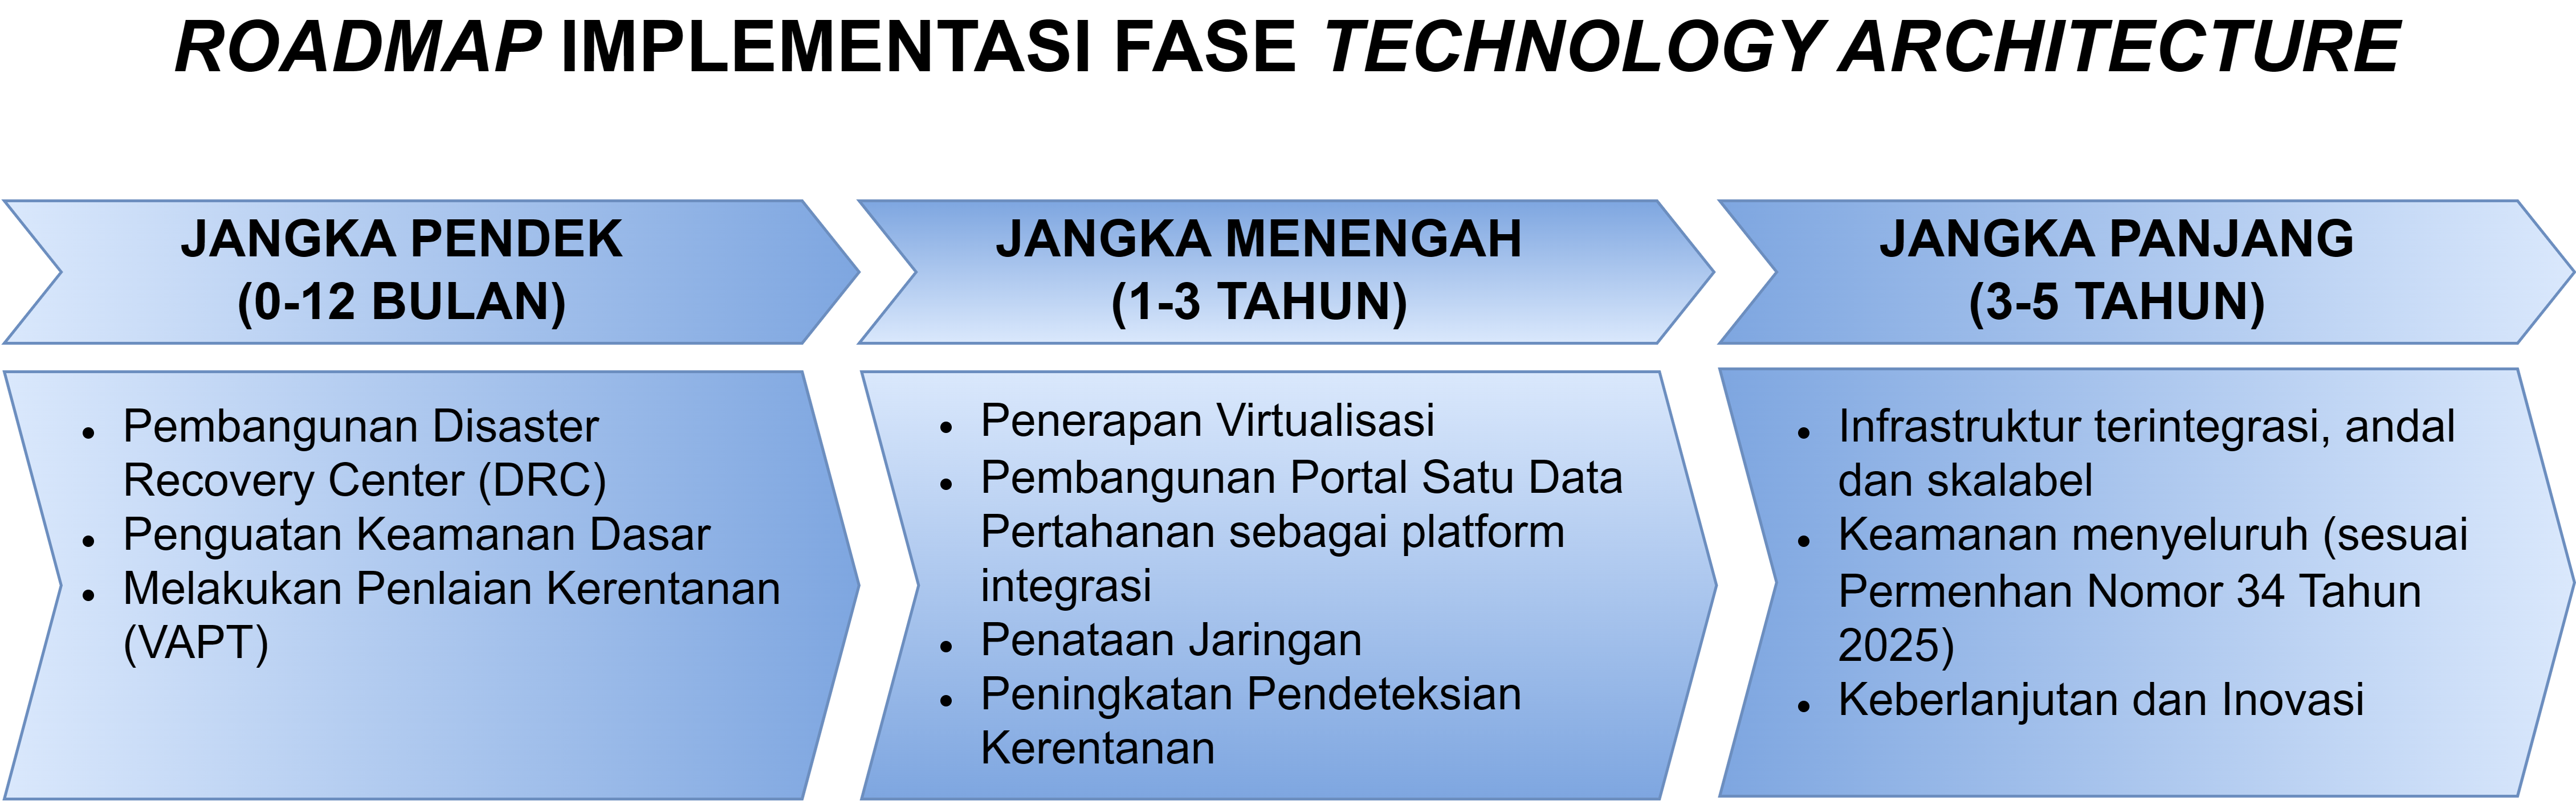
\includegraphics[width=0.99\linewidth,height=0.8\textheight,keepaspectratio]{images/Roadmap implementasi fase Technology Architecture.drawio.drawio.png}
\caption{\textit{Roadmap} Implementasi Fase \textit{Technology Architecture}}
\label{fig:IV.15}
\end{figure}

Gambar~\ref{fig:IV.15} menunjukkan bahwa jangka pendek (0–12 bulan) difokuskan pada pembangunan DRC beserta cadangan dan replikasi data, penguatan keamanan dasar (\textit{firewall}, \textit{endpoint protection}, dan IDPS), serta penilaian kerentanan melalui VAPT. Jangka menengah (1–3 tahun) menerapkan virtualisasi dan kontainer, membangun lapisan integrasi dan Portal Satu Data Pertahanan, menata jaringan tersegmentasi, serta memperkuat deteksi melalui CTI, SIEM, dan SOAR. Jangka panjang (3–5 tahun) mengoperasikan \textit{Data Center} Utama dan DRC secara aktif-aktif, memperluas interoperabilitas lintas matra, dan mencapai kematangan keamanan level 3.

\section{Fase C6ISR Architecture}
\label{sec:IV.6}

Fase C6ISR Architecture merancang kapabilitas \textit{Command, Control, Communications, Computers, Cyber-Defense, Combat Systems, Intelligence, Surveillance, and Reconnaissance} (C6ISR) sebagai inti operasional pertahanan cerdas. Fase ini merupakan fase khusus TOGAF Pertahanan Indonesia yang menerjemahkan kebutuhan operasional pertahanan menjadi satu kesatuan arsitektur C6ISR. Fase ini ditempatkan setelah Fase \textit{Technology Architecture} karena memanfaatkan fondasi data, aplikasi, jaringan, komputasi, dan keamanan yang telah dirancang sebelumnya.

Arsitektur C6ISR dirancang dari sudut pandang Kemhan RI, yaitu kebijakan, standar interoperabilitas, persyaratan pengadaan alutsista, dan sumber daya yang memungkinkan kapabilitas C6ISR terwujud. Komando dan pengendalian penggunaan kekuatan tetap berada pada Mabes TNI, sehingga fase ini tidak memodelkan prosedur operasi TNI. Pendekatan yang digunakan adalah \textit{Network Centric Warfare} \cite{Koch2015}, yaitu menghubungkan sumber informasi, komunikasi, komputasi, intelijen, komando-kendali, dan unsur penindak melalui jaringan yang interoperabel.

Pemodelan dilakukan pada tingkat konseptual berdasarkan doktrin, kebijakan, dan sumber terbuka. Penelitian ini tidak mencakup spesifikasi teknis alutsista, konfigurasi persandian, maupun gelar kekuatan.

\subsection{Kebutuhan Operasional}
\label{sec:IV.6.1}

Kebutuhan operasional (KO) C6ISR diturunkan dari doktrin dan dokumen kebijakan pertahanan, sebagaimana disajikan pada Tabel~\ref{tab:IV.23}.

\begingroup\small\setstretch{1.0}
\begin{longtable}{@{}>{\raggedright\arraybackslash\hspace{0pt}}p{0.097\linewidth}>{\raggedright\arraybackslash\hspace{0pt}}p{0.389\linewidth}>{\raggedright\arraybackslash\hspace{0pt}}p{0.214\linewidth}>{\raggedright\arraybackslash\hspace{0pt}}p{0.207\linewidth}@{}}
\caption{Kebutuhan Operasional C6ISR}\label{tab:IV.23}\\
\toprule
\textbf{Kode} & \textbf{Kebutuhan Operasional} & \textbf{Sumber} & \textbf{Elemen C6ISR}\\
\midrule
\endfirsthead
\multicolumn{4}{@{}l}{\small\itshape \tablename\ \thetable{} (lanjutan)}\\
\toprule
\textbf{Kode} & \textbf{Kebutuhan Operasional} & \textbf{Sumber} & \textbf{Elemen C6ISR}\\
\midrule
\endhead
\bottomrule
\endlastfoot
\centering\arraybackslash KO-01 & Integrasi C6ISR ketiga matra dalam satu pusat komando dan kendali berbasis \textit{network centric warfare} & Kajian Ditjen Pothan Kemhan \cite{Dwipratama2023} & \textit{Command, Control, Communications}\\
\centering\arraybackslash KO-02 & Modernisasi alutsista yang terintegrasi dengan konsep \textit{network centric warfare} & Permenhan Nomor 12 Tahun 2021 \cite{Permenhan12Tahun2021} & \textit{Combat Systems}\\
\centering\arraybackslash KO-03 & Siklus \textit{sense}, \textit{make sense}, dan \textit{act} yang cepat lintas domain, dengan kemampuan bertindak mandiri saat komunikasi terganggu & Strategi JADC2 \cite{USDoD2022} & \textit{Command, Control, Computers}\\
\centering\arraybackslash KO-04 & Perlindungan terhadap ancaman perangkat keras (termasuk \textit{jamming}), perangkat lunak, serta data dan informasi & Pedoman Pertahanan Siber \cite{Permenhan82Tahun2014} & \textit{Cyber-Defense, Communications}\\
\centering\arraybackslash KO-05 & Jalur komunikasi satelit yang terjamin kerahasiaan dan kemandiriannya & Kajian Ditjen Pothan Kemhan \cite{Dwipratama2023} & \textit{Communications}\\
\centering\arraybackslash KO-06 & Pelindungan infrastruktur informasi vital dengan target kematangan keamanan siber level 3 pada tahun 2029 & Permenhan Nomor 34 Tahun 2025 \cite{Permenhan34Tahun2025} & \textit{Cyber-Defense}\\
\centering\arraybackslash KO-07 & Pengamanan data sesuai klasifikasi Terbuka, Terbatas, dan Rahasia & Permenhan Nomor 1 Tahun 2023 \cite{Permenhan1Tahun2023} & \textit{Computers, Cyber-Defense}\\
\end{longtable}
\endgroup

Tabel~\ref{tab:IV.23} menunjukkan bahwa ketujuh kebutuhan operasional mencakup seluruh elemen C6ISR.

\subsection{Arsitektur C6ISR \textit{Baseline}}
\label{sec:IV.6.2}

Data rinci mengenai sistem komando dan kendali, sensor, dan alutsista ketiga matra bersifat terbatas. Oleh karena itu, arsitektur C6ISR \textit{baseline} disusun sebagai model logis berdasarkan sumber terbuka. Model ini menggambarkan kondisi umum dan tidak merepresentasikan konfigurasi aktual setiap sistem pertahanan, sebagaimana ditunjukkan pada Gambar~\ref{fig:IV.16}.
\begin{figure}[htbp]
\centering
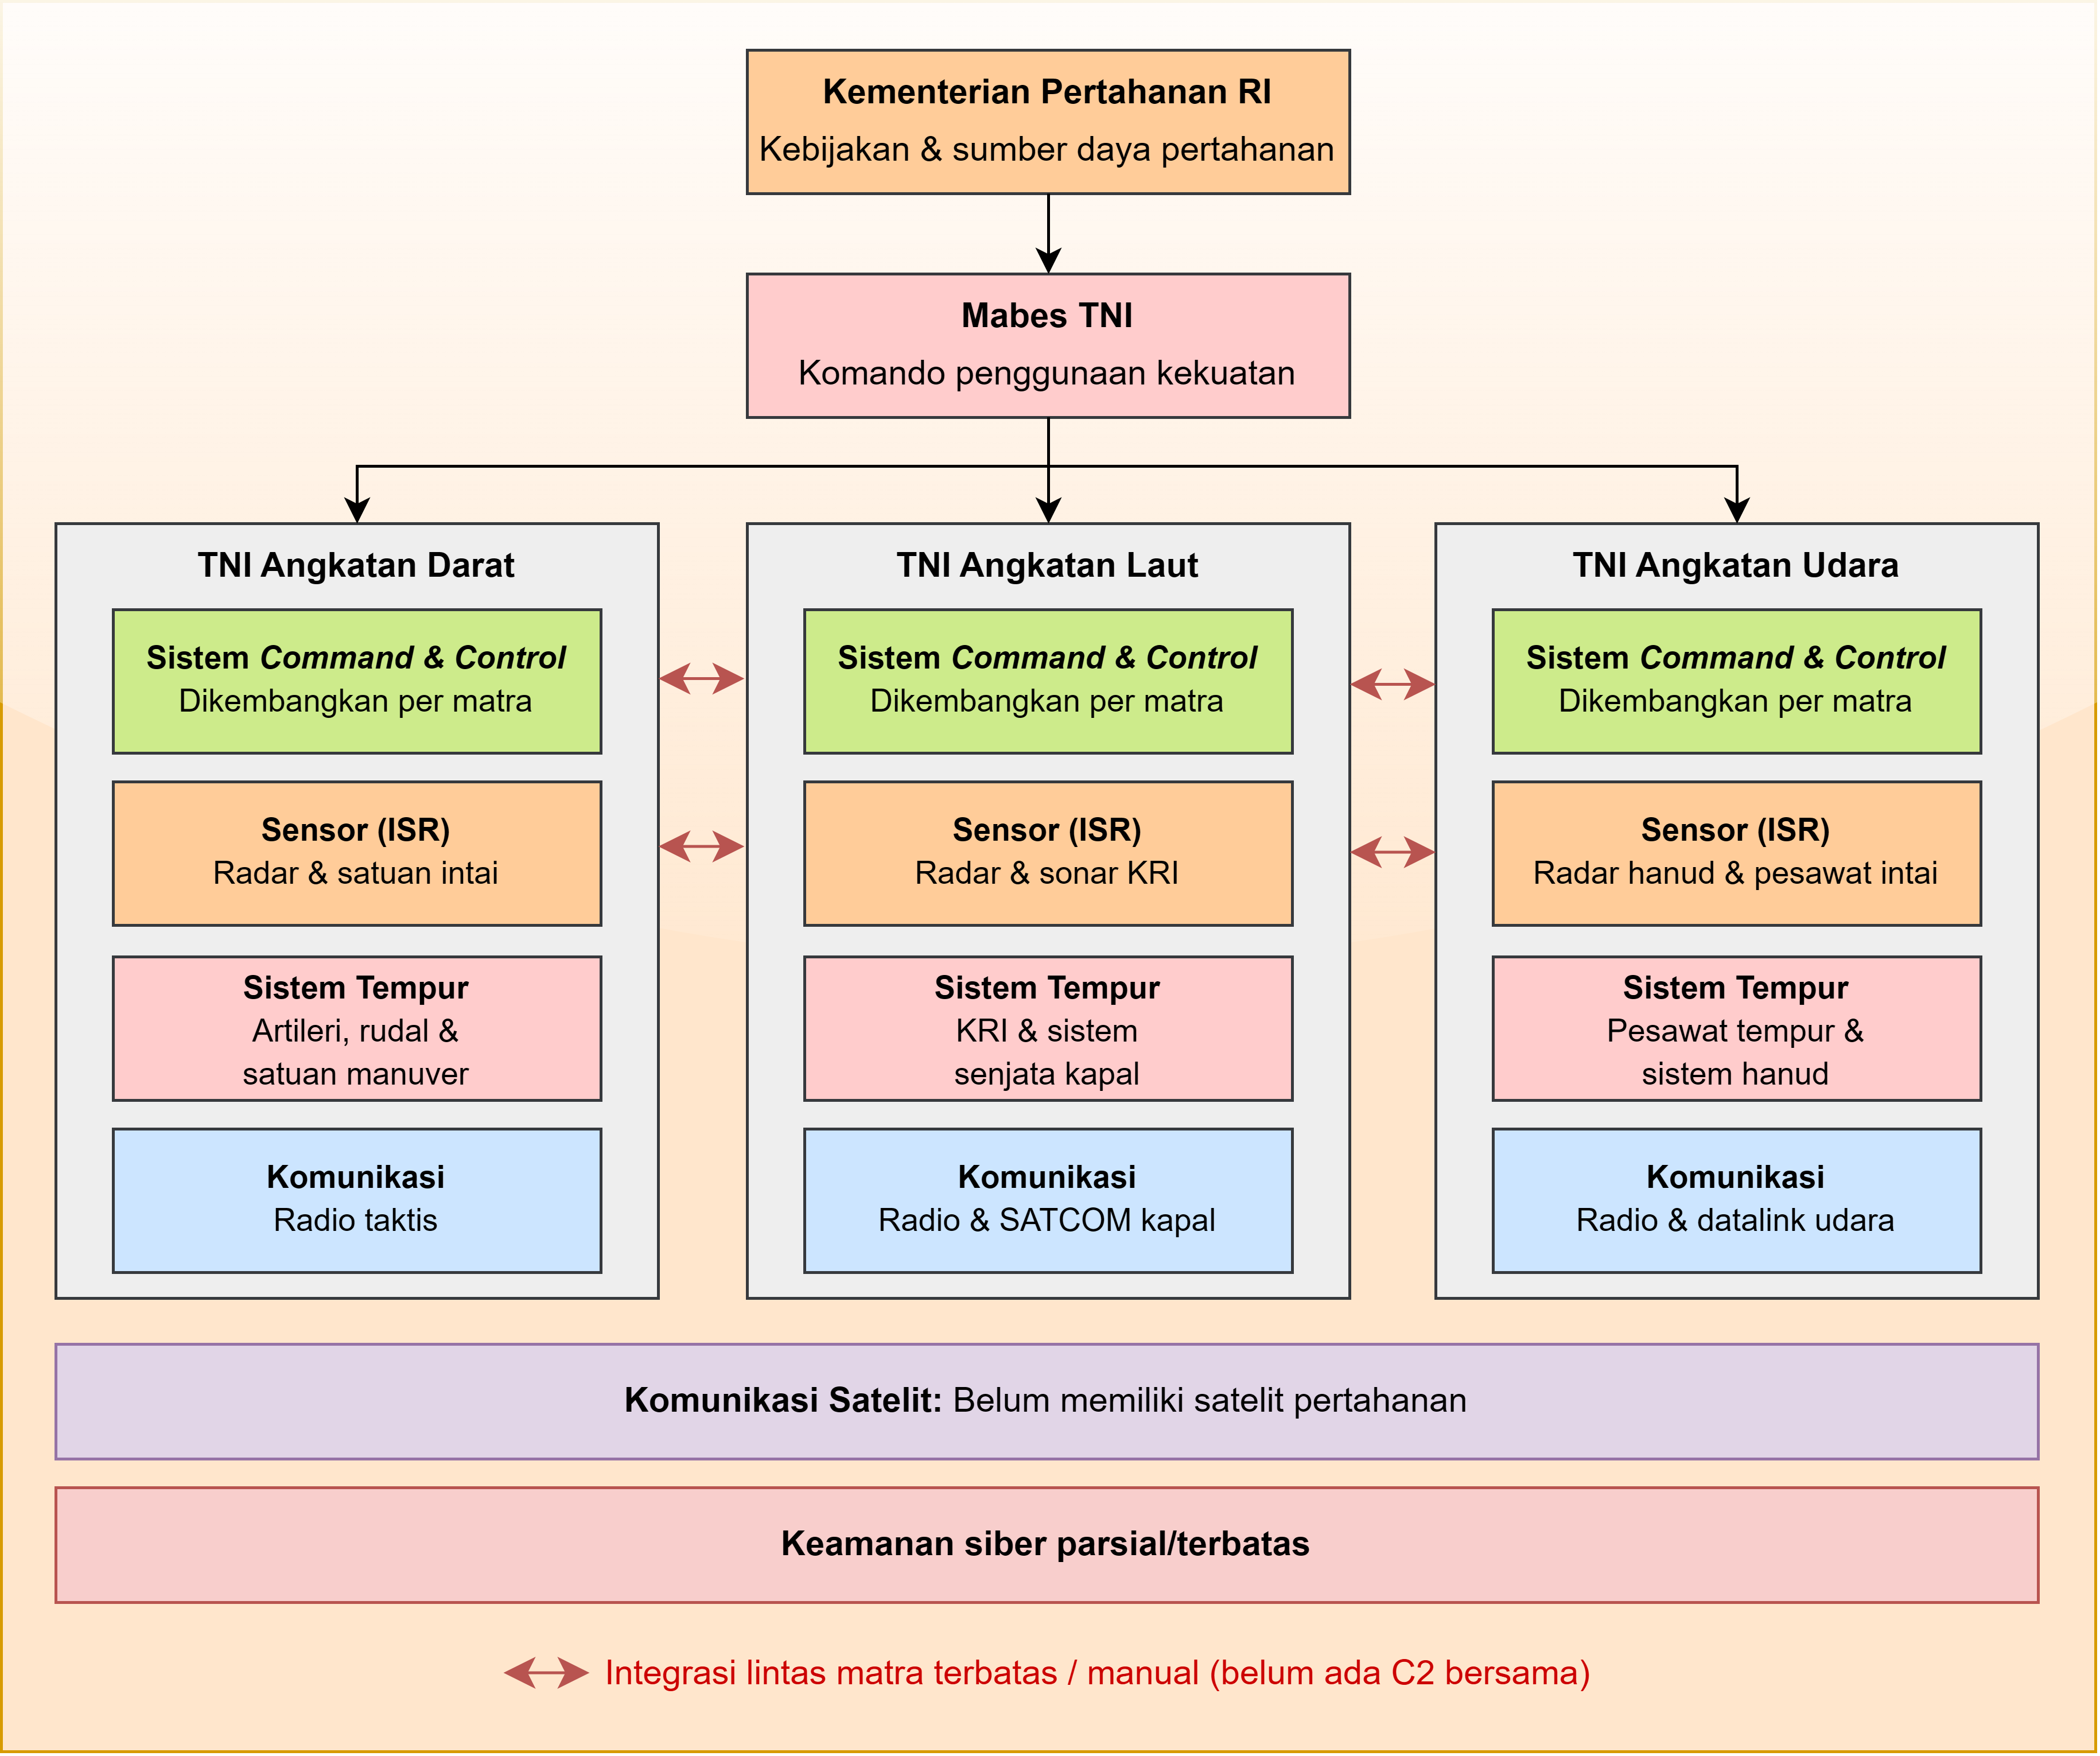
\includegraphics[width=0.93\linewidth,height=0.8\textheight,keepaspectratio]{images/C6ISR Baseline.drawio.png}
\caption{Arsitektur C6ISR \textit{Baseline}}
\label{fig:IV.16}
\end{figure}

Gambar~\ref{fig:IV.16} menunjukkan bahwa setiap matra memiliki sistem \textit{Command \& Control}, sensor, sistem tempur, dan sarana komunikasi sendiri, sedangkan integrasi antarmatra masih terbatas dan sebagian dilakukan secara manual. Kondisi setiap elemen C6ISR dirangkum pada Tabel~\ref{tab:IV.24}.

\begingroup\small\setstretch{1.0}
\begin{longtable}{@{}>{\raggedright\arraybackslash\hspace{0pt}}p{0.067\linewidth}>{\raggedright\arraybackslash\hspace{0pt}}p{0.221\linewidth}>{\raggedright\arraybackslash\hspace{0pt}}p{0.649\linewidth}@{}}
\caption{Kondisi C6ISR \textit{Baseline}}\label{tab:IV.24}\\
\toprule
\textbf{No.} & \textbf{Elemen} & \textbf{Kondisi \textit{Baseline}}\\
\midrule
\endfirsthead
\multicolumn{3}{@{}l}{\small\itshape \tablename\ \thetable{} (lanjutan)}\\
\toprule
\textbf{No.} & \textbf{Elemen} & \textbf{Kondisi \textit{Baseline}}\\
\midrule
\endhead
\bottomrule
\endlastfoot
\centering\arraybackslash 1 & \textit{Command \& Control} & Sistem dikembangkan per matra; belum ada aplikasi \textit{Command \& Control} lintas matra\\
\centering\arraybackslash 2 & \textit{Communications} & Belum memiliki satelit pertahanan dan hak slot orbit 123° BT tidak lagi dimiliki sejak Desember 2024 \cite{SuaraMerdeka2026}; jaringan belum tersegmentasi dan belum lintas matra\\
\centering\arraybackslash 3 & \textit{Computers} & Satu \textit{Data Center} tanpa DRC; aplikasi bersifat \textit{silo}; belum ada fusi data dan analitik operasional\\
\centering\arraybackslash 4 & \textit{Cyber Defense} & Keamanan siber parsial dengan kematangan level 1–2; belum ada pemisahan jaringan operasional terklasifikasi\\
\centering\arraybackslash 5 & \textit{Combat Systems} & Alutsista berasal dari berbagai negara produsen dengan standar antarmuka beragam, sehingga integrasi dengan \textit{Command \& Control} lintas matra terbatas\\
\centering\arraybackslash 6 & ISR & Sensor dikelola per matra dan datanya belum difusikan lintas matra; belum ada satelit ISR khusus pertahanan\\
\end{longtable}
\endgroup

Tabel~\ref{tab:IV.24} menunjukkan tiga karakteristik utama. Pertama, kapabilitas C6ISR masih terpisah per matra sehingga belum terbentuk gambaran situasi bersama. Kedua, komunikasi belum didukung satelit yang dikuasai sendiri, padahal wilayah Indonesia luas dan berbentuk kepulauan. Ketiga, perbedaan standar sistem tempur menyebabkan alur ISR–komando-kendali–unsur penindak belum terbentuk secara utuh.

\subsection{Peta Kapabilitas C6ISR}
\label{sec:IV.6.3}

Peta kapabilitas C6ISR menunjukkan kemampuan yang dibutuhkan untuk menjalankan seluruh proses C6ISR, tanpa bergantung pada unit atau sistem yang melaksanakannya. Peta ini merinci kapabilitas Manajemen Komando dan Koordinasi pada Gambar~\ref{fig:IV.5}, sebagaimana disajikan pada Gambar~\ref{fig:IV.17}.
\begin{figure}[htbp]
\centering
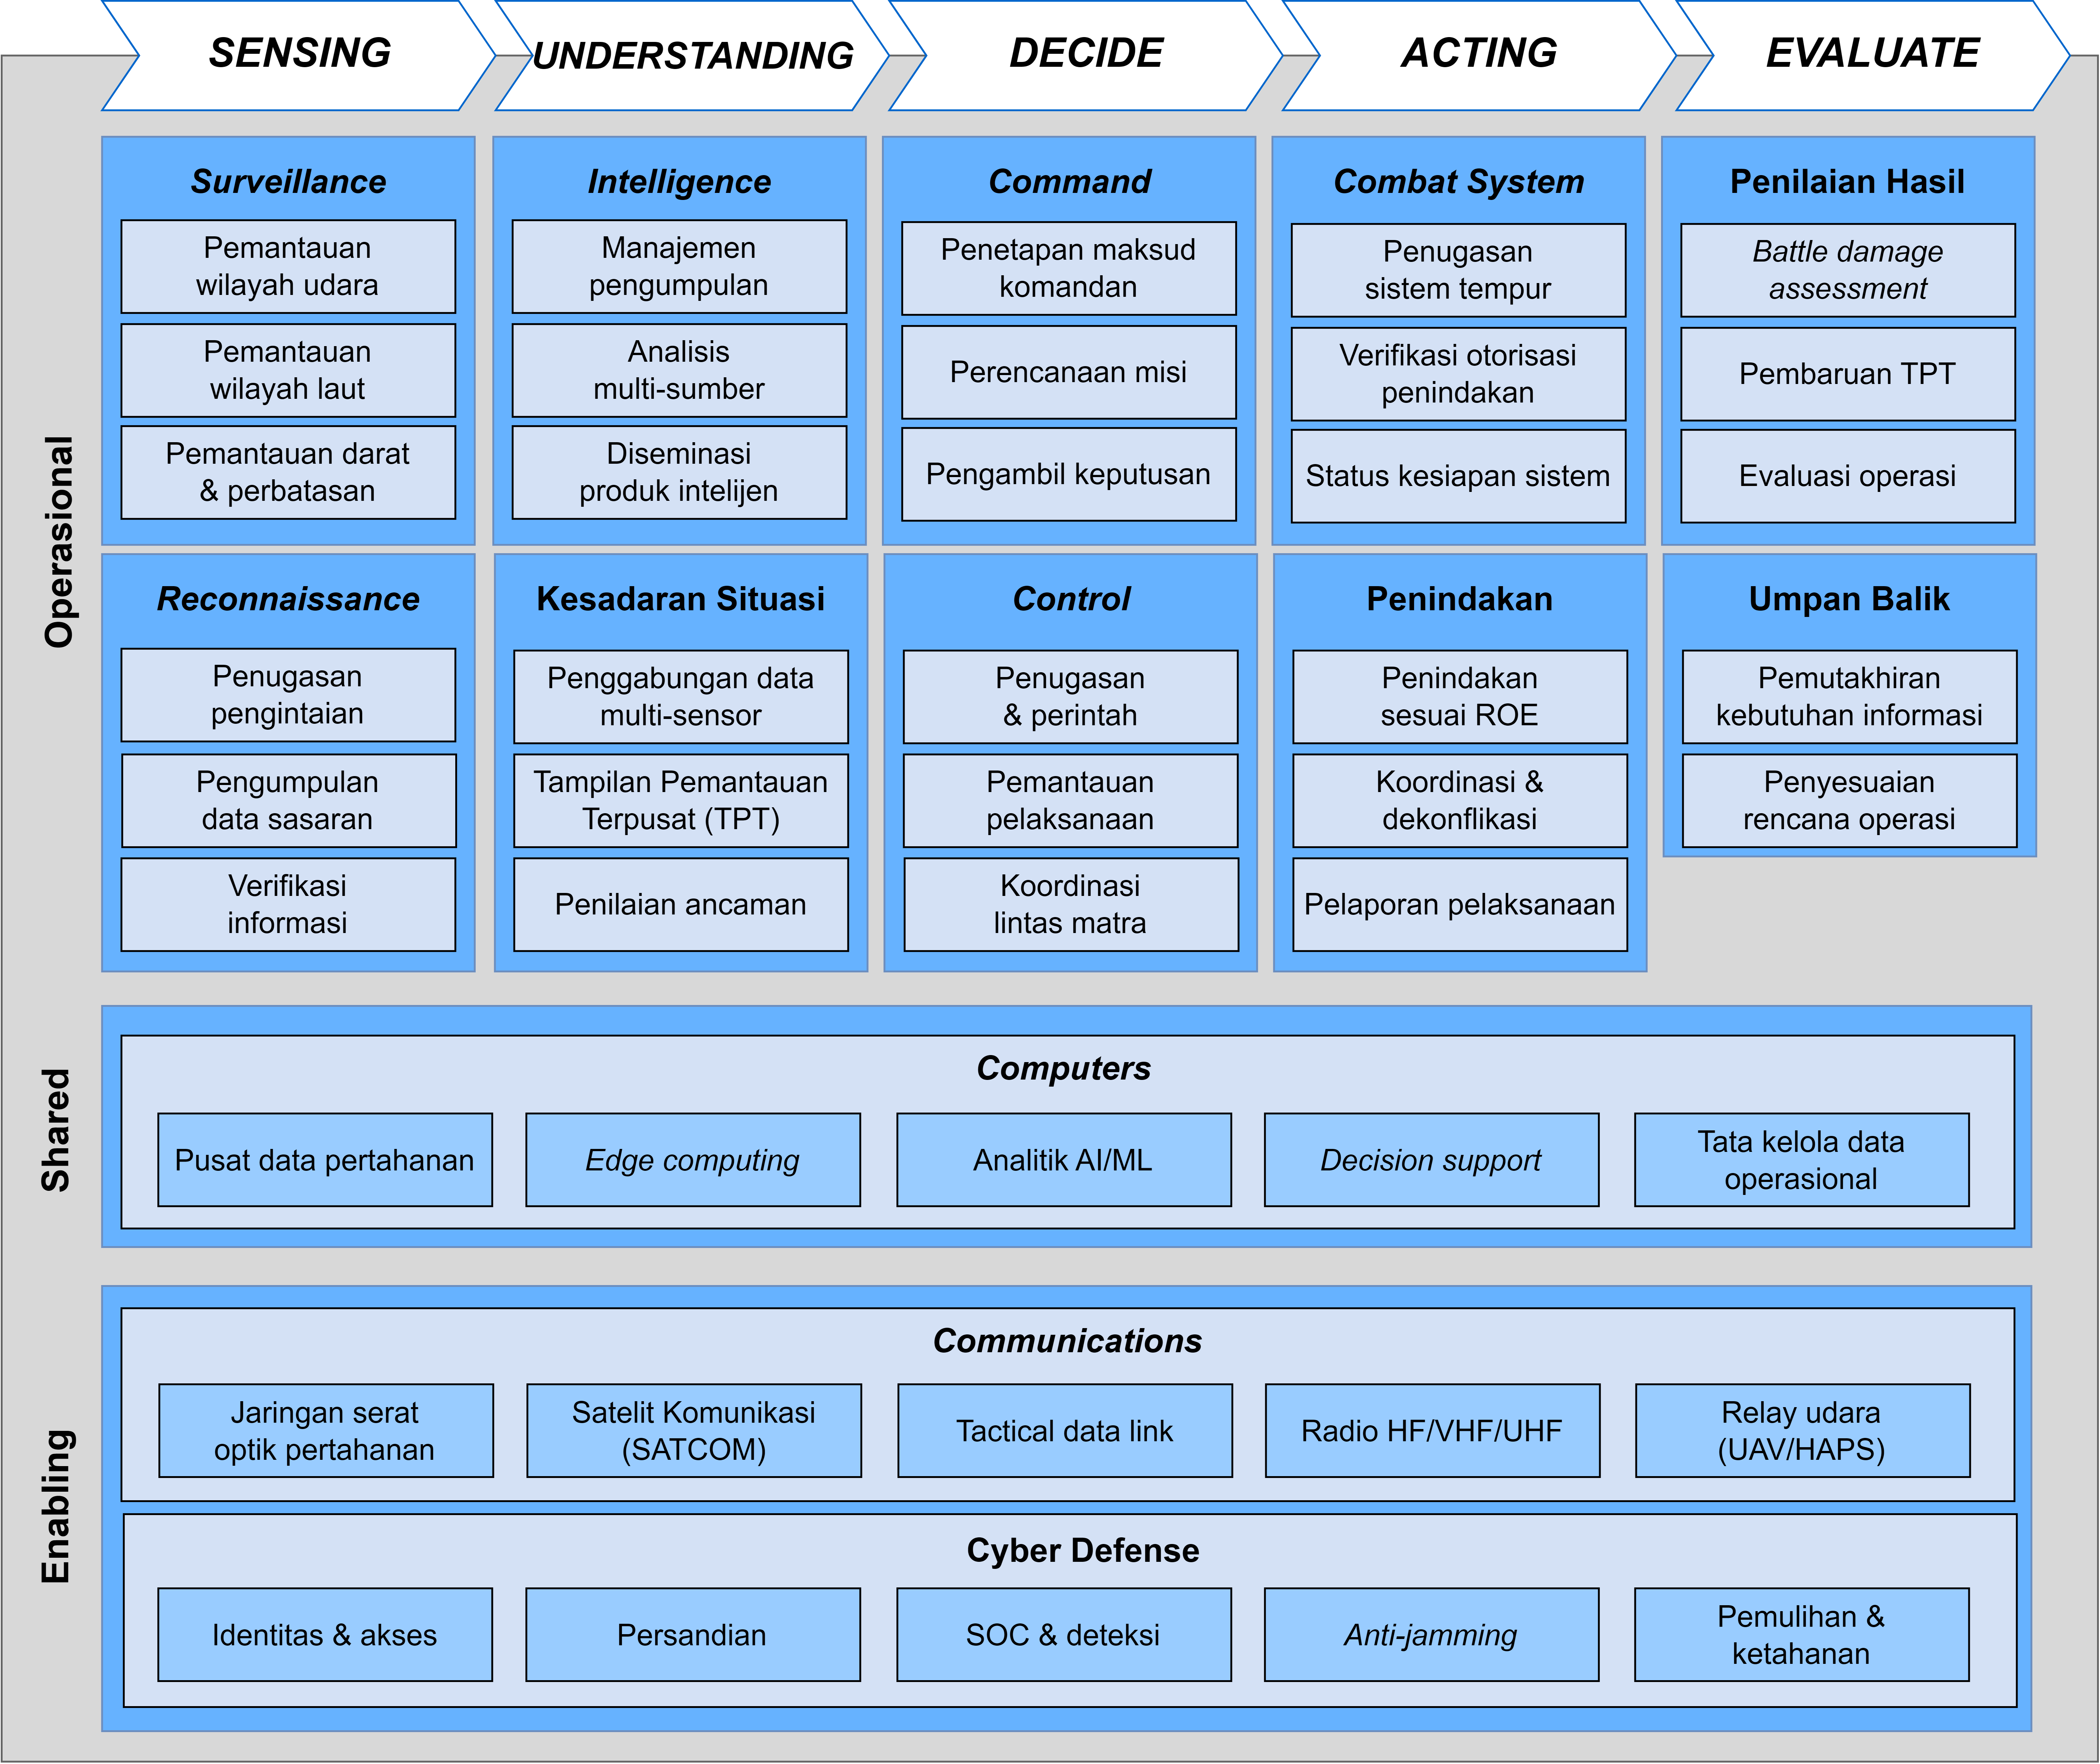
\includegraphics[width=0.99\linewidth,height=0.8\textheight,keepaspectratio]{images/Kapabilitas C6ISR.drawio.png}
\caption{Peta Kapabilitas C6ISR (\textit{C6ISR Capability Map})}
\label{fig:IV.17}
\end{figure}

Gambar~\ref{fig:IV.17} membagi kapabilitas C6ISR ke dalam tiga lapis. Lapis operasional mengikuti siklus \textit{sensing}, \textit{understanding}, \textit{decide}, \textit{acting}, dan \textit{evaluate}. Siklus dimulai dari \textit{surveillance} dan \textit{reconnaissance}, dilanjutkan dengan \textit{intelligence} dan kesadaran situasi, \textit{command} dan \textit{control}, serta \textit{combat system} dan penindakan. Siklus diakhiri dengan penilaian hasil dan umpan balik yang memperbarui Tampilan Pemantauan Terpusat (TPT) dan rencana operasi, sehingga siklus dapat dimulai kembali.

Lapis \textit{shared} berisi kapabilitas \textit{computers}, yaitu pusat data pertahanan, \textit{edge computing}, analitik AI/ML, \textit{decision support}, dan tata kelola data operasional. Lapis \textit{enabling} berisi kapabilitas \textit{communications} dan \textit{cyber defense} yang menopang konektivitas dan perlindungan pada seluruh siklus.

\subsection{Arsitektur C6ISR Target}
\label{sec:IV.6.4}

Arsitektur C6ISR target dirancang untuk menutup kesenjangan \textit{baseline} dengan menerapkan model C6ISR pada konteks pertahanan Indonesia, sebagaimana ditunjukkan pada Gambar~\ref{fig:IV.18}.
\begin{figure}[htbp]
\centering
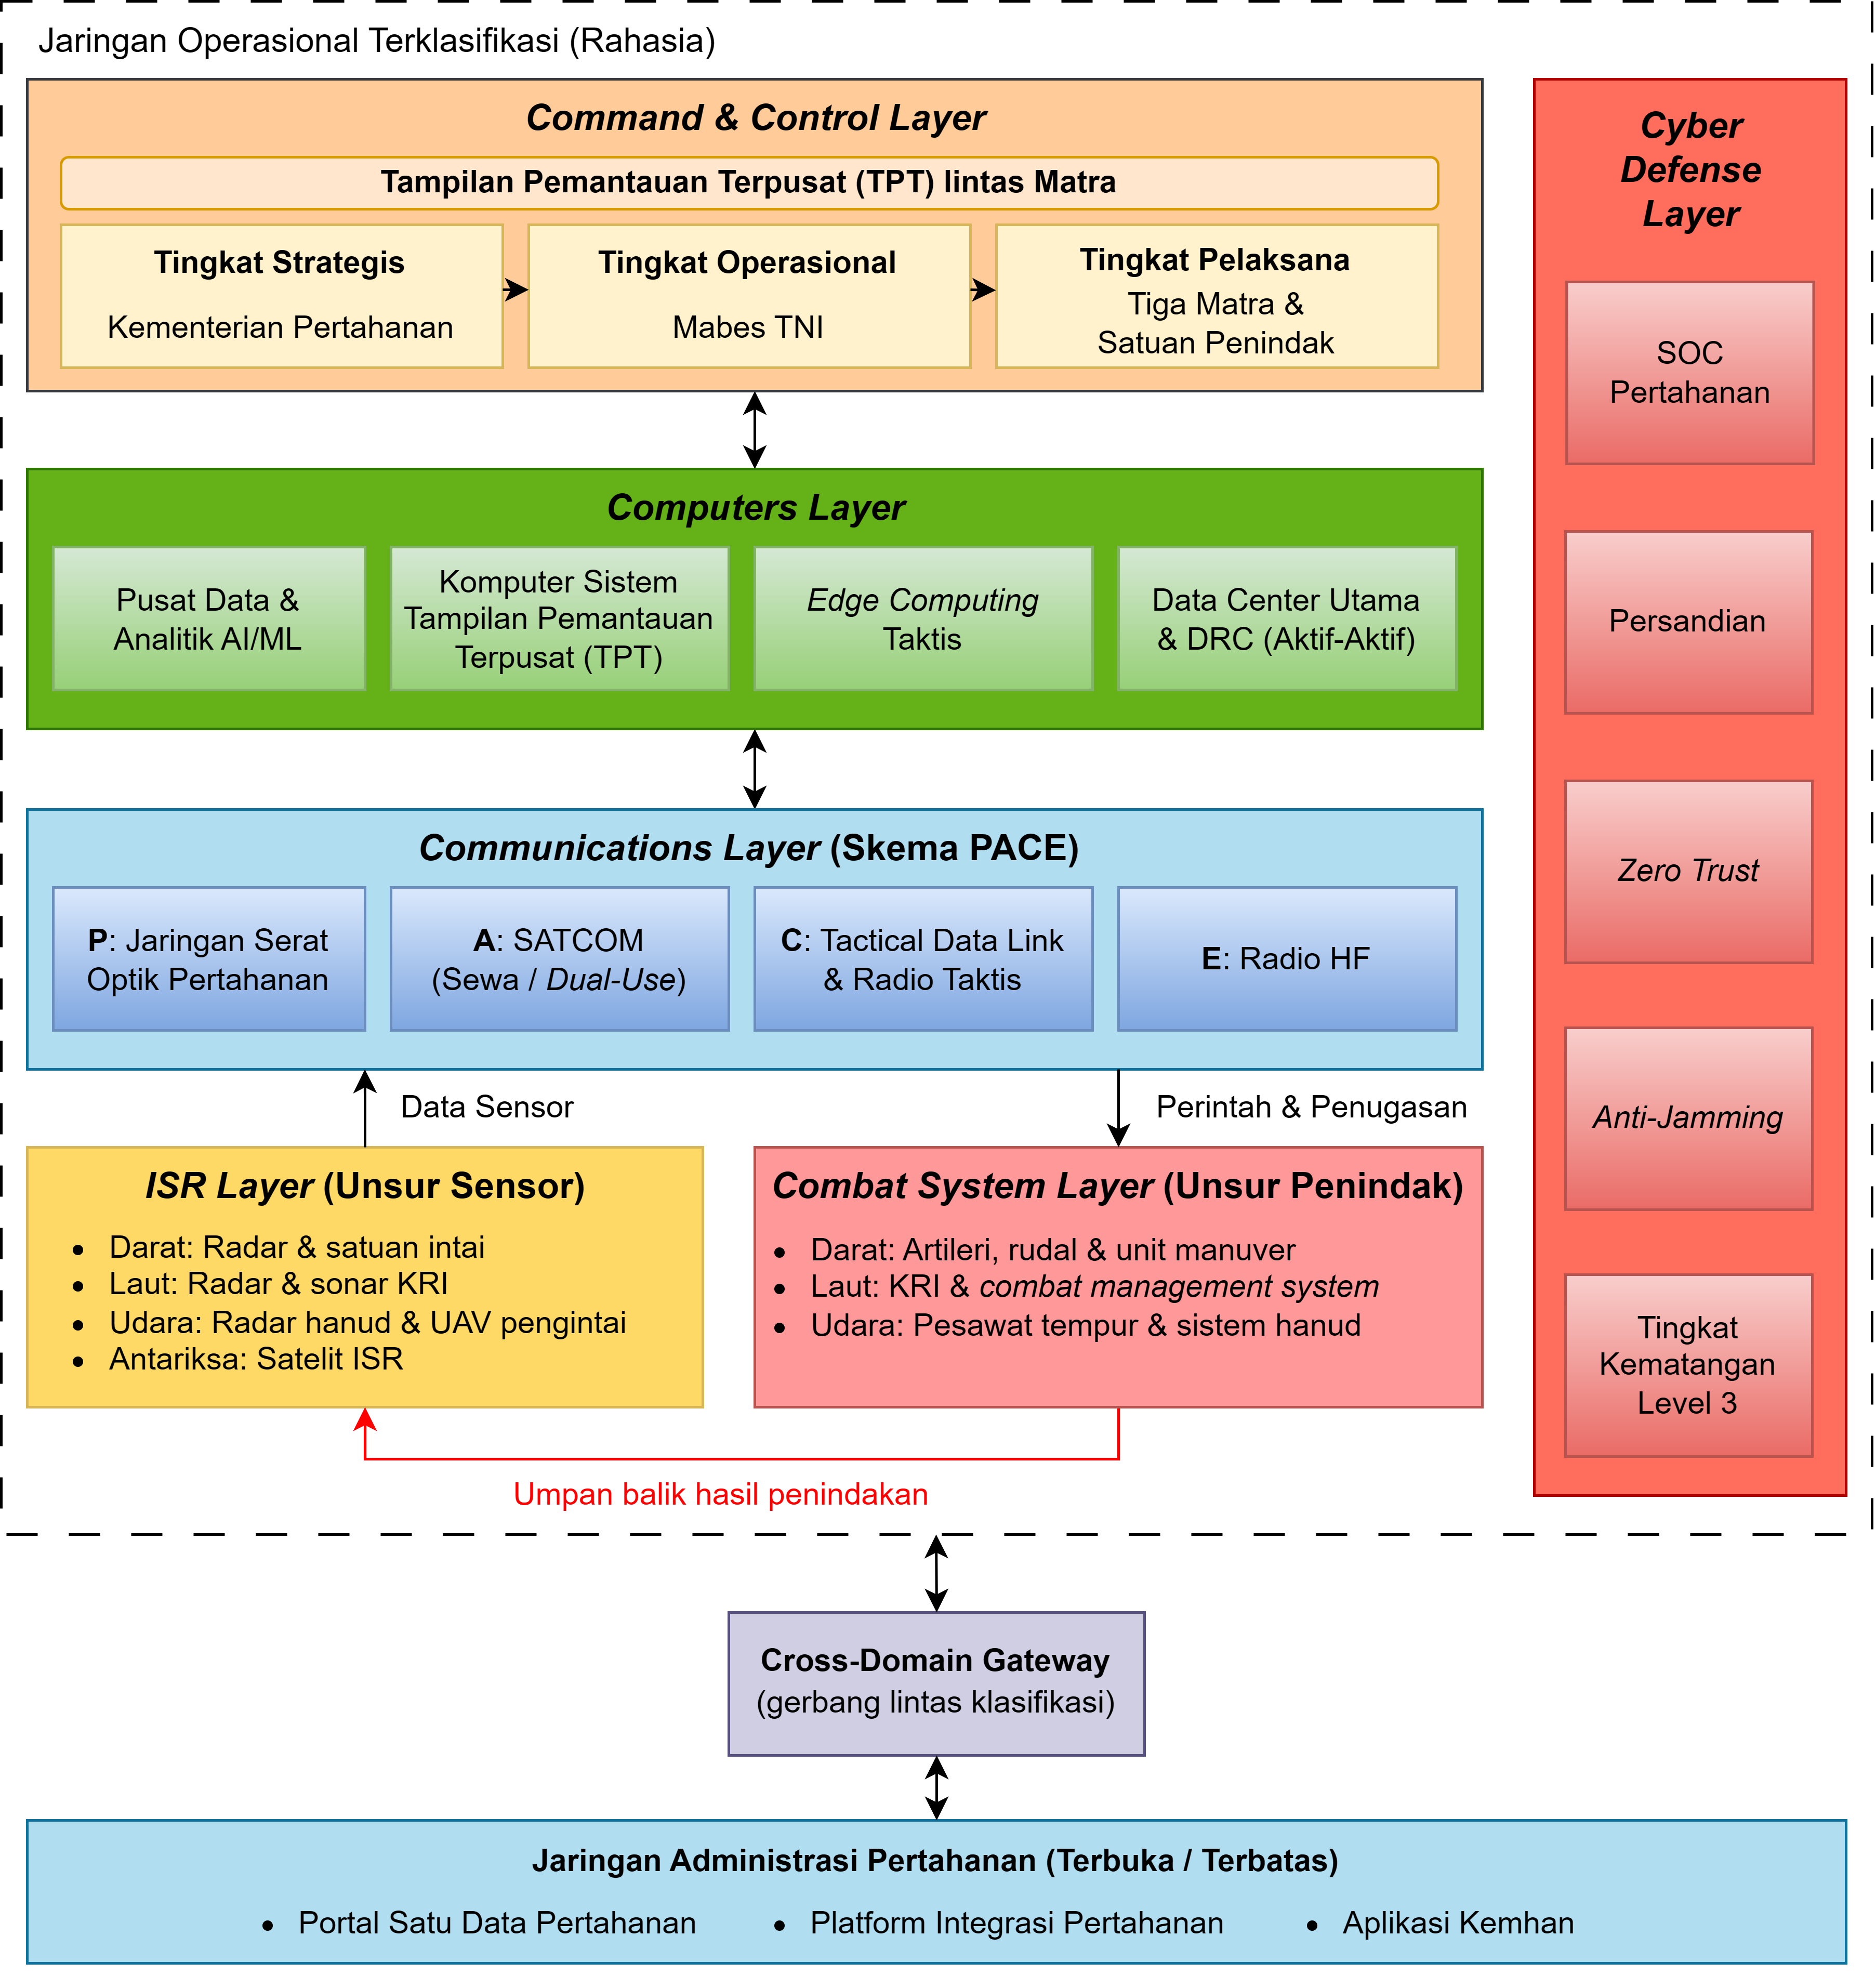
\includegraphics[width=0.89\linewidth,height=0.8\textheight,keepaspectratio]{images/C6ISR Target.drawio.png}
\caption{Arsitektur C6ISR Target}
\label{fig:IV.18}
\end{figure}

Gambar~\ref{fig:IV.18} menunjukkan bahwa data dari \textit{ISR Layer} dikirim melalui \textit{Communications Layer} ke \textit{Computers Layer} untuk diolah dan ditampilkan pada TPT di \textit{Command \& Control Layer}. Perintah dan penugasan disalurkan kembali melalui \textit{Communications Layer} kepada \textit{Combat Systems Layer}, sedangkan hasil penindakan dikembalikan ke \textit{ISR Layer} sebagai umpan balik. Alur ini membentuk siklus tertutup dari pengindraan hingga penindakan. \textit{Cyber Defense Layer} digambarkan vertikal karena melekat pada seluruh lapisan.

Seluruh lapisan C6ISR ditempatkan pada jaringan operasional terklasifikasi (Rahasia) yang terpisah dari jaringan administrasi pertahanan (Terbuka dan Terbatas). Pertukaran informasi antara kedua jaringan dilakukan melalui \textit{Cross-Domain Gateway}, sehingga data operasional harus melalui proses pengendalian sebelum digunakan pada jaringan administrasi. Rincian setiap lapisan diuraikan sebagai berikut.

\subsubsection{\textit{Command \& Control Layer}}
\label{sec:IV.6.4.1}

\textit{Command \& Control} dirancang berjenjang dalam tiga tingkat, yaitu strategis, operasional, dan pelaksana. Setiap tingkat menggunakan gambaran situasi yang sama, tetapi informasinya disesuaikan dengan kewenangan masing-masing, sebagaimana diilustrasikan pada Gambar~\ref{fig:IV.19}.
\begin{figure}[htbp]
\centering
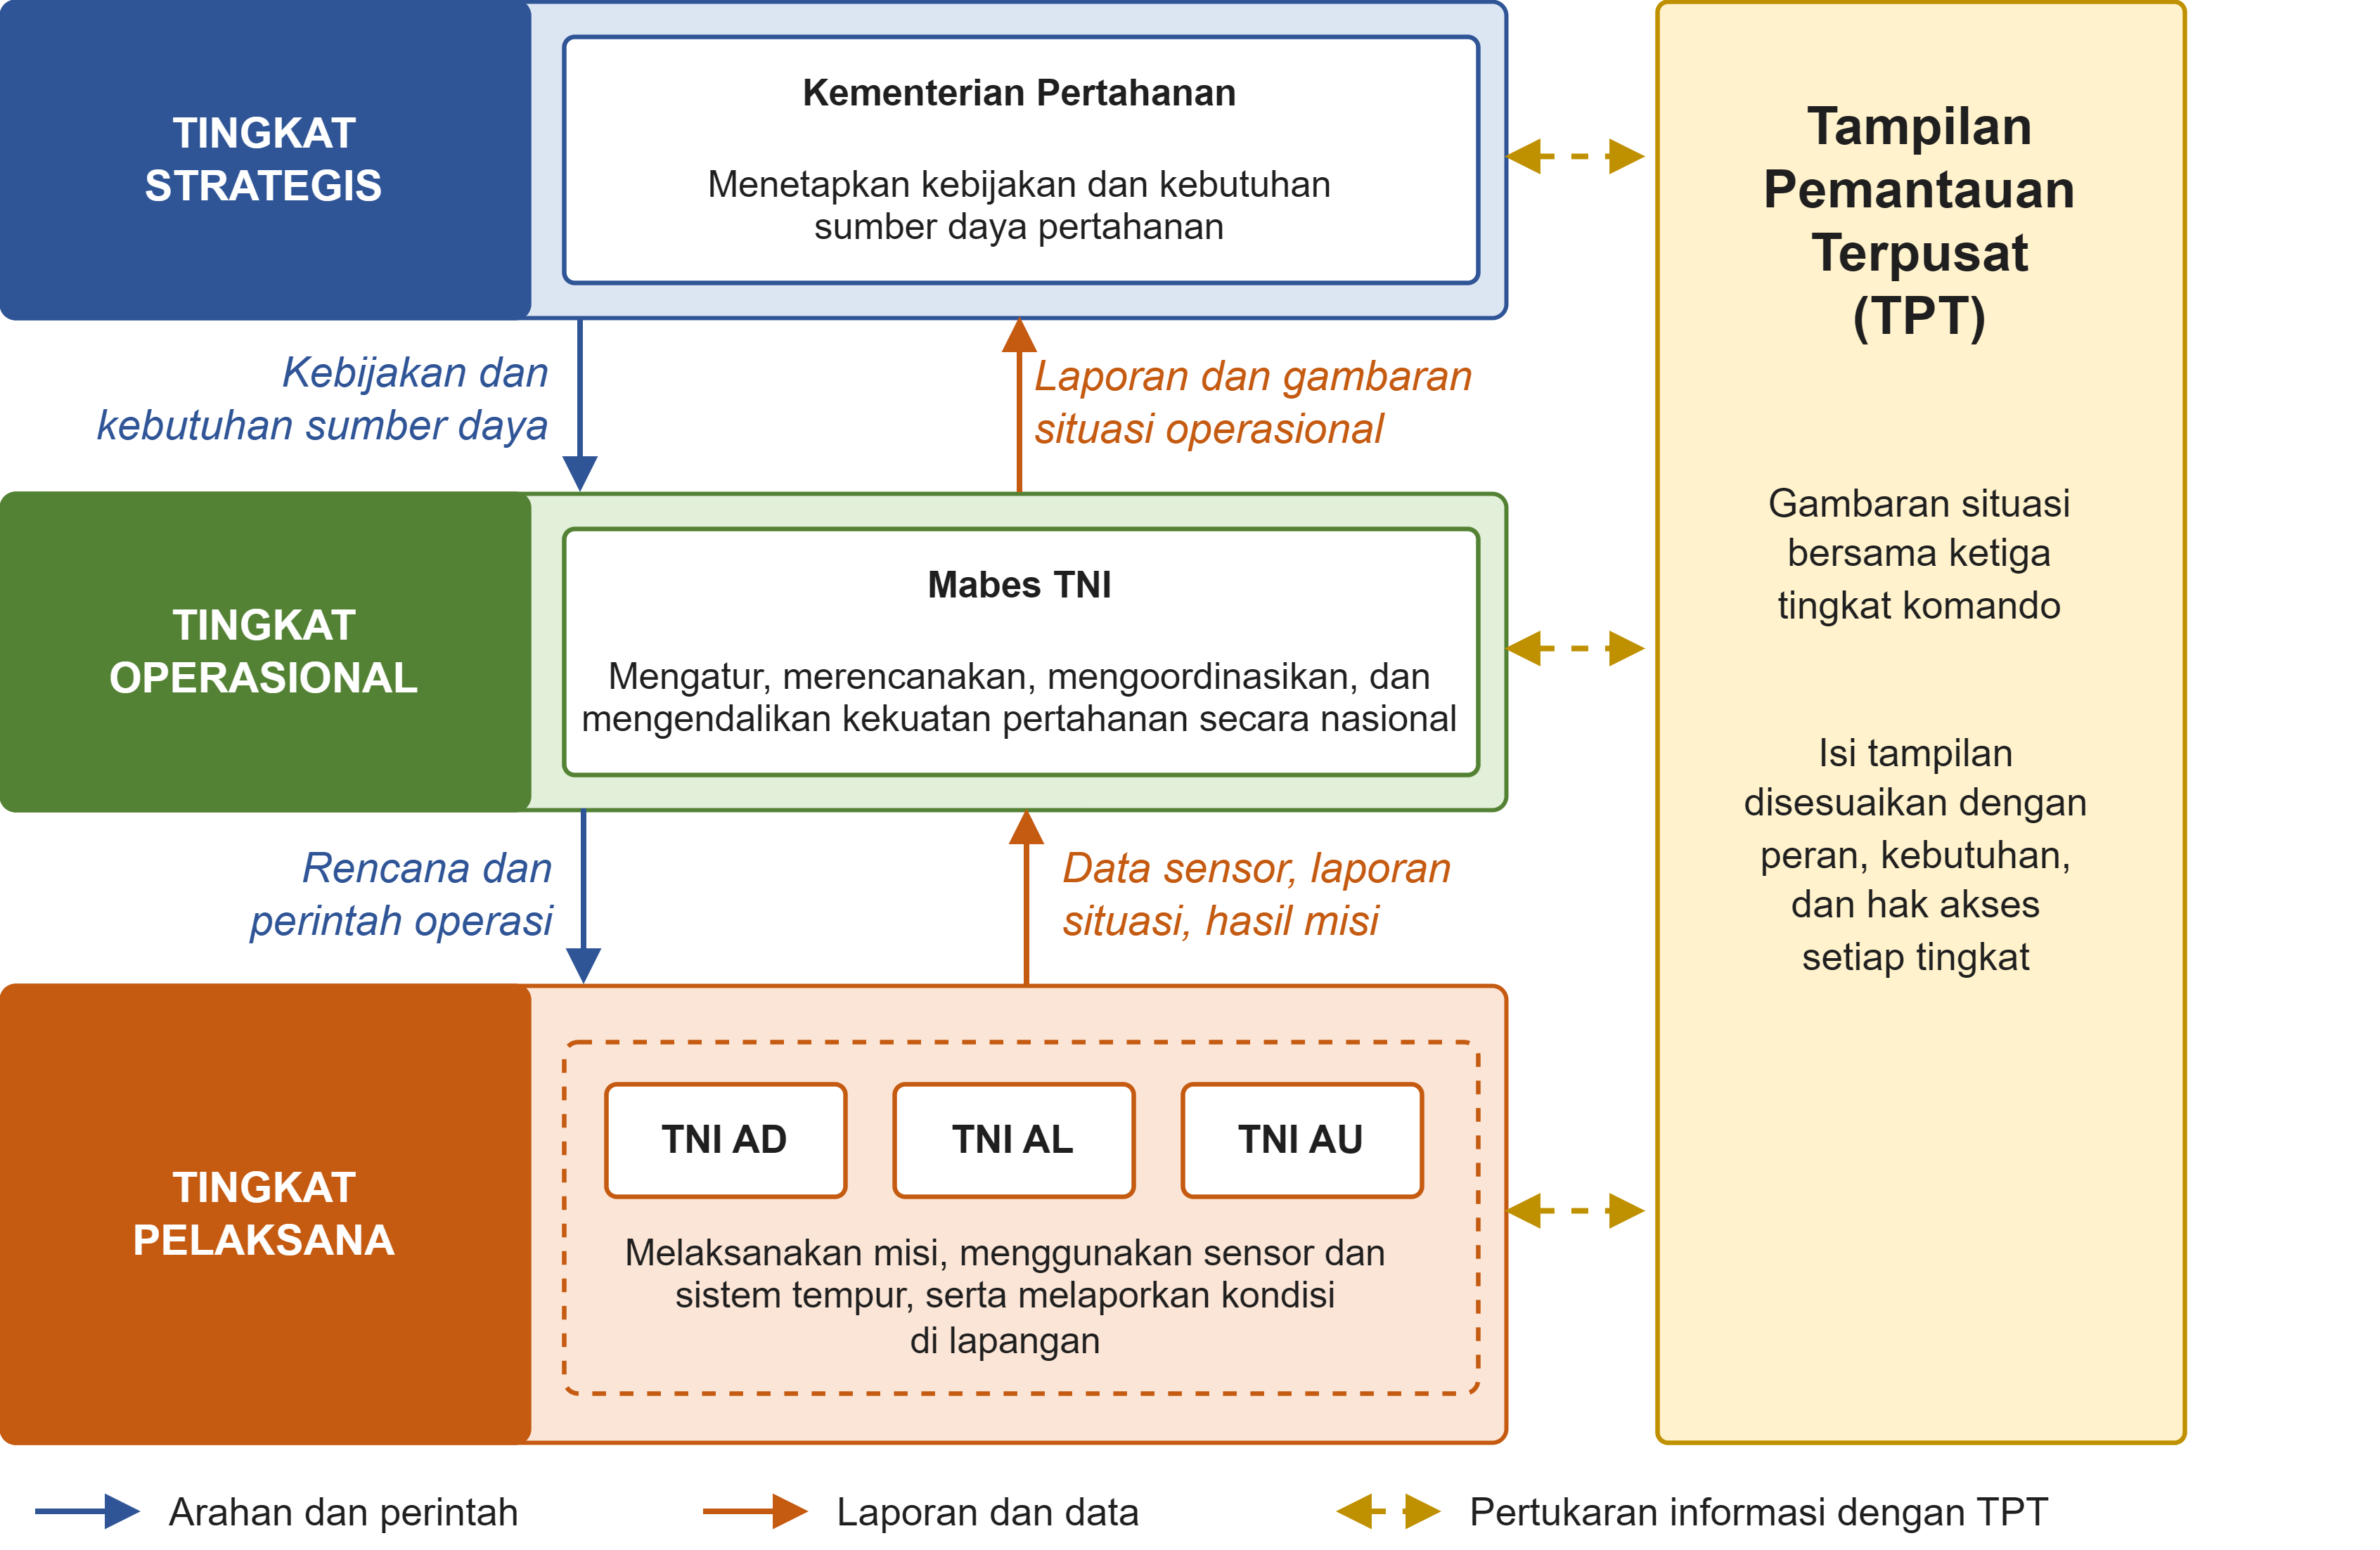
\includegraphics[width=0.99\linewidth,height=0.8\textheight,keepaspectratio]{images/Tingkat_Command_Control_C6ISR.drawio.png}
\caption{Tingkatan \textit{Command \& Control} C6ISR}
\label{fig:IV.19}
\end{figure}

Gambar~\ref{fig:IV.19} menunjukkan dua arah aliran. Arahan mengalir dari atas ke bawah, yaitu Kemhan menyampaikan kebijakan dan kebutuhan sumber daya kepada Mabes TNI, kemudian Mabes TNI menjabarkannya menjadi rencana dan perintah operasi bagi ketiga matra. Laporan mengalir dari bawah ke atas, yaitu ketiga matra mengirimkan data sensor, laporan situasi, dan hasil misi kepada Mabes TNI, yang kemudian menyampaikan gambaran situasi operasional kepada Kemhan. Setiap tingkat juga bertukar informasi dua arah dengan TPT. Peran dan produk informasi setiap tingkat disajikan pada Tabel~\ref{tab:IV.25}.

\begingroup\small\setstretch{1.0}
\begin{longtable}{@{}>{\raggedright\arraybackslash\hspace{0pt}}p{0.155\linewidth}>{\raggedright\arraybackslash\hspace{0pt}}p{0.181\linewidth}>{\raggedright\arraybackslash\hspace{0pt}}p{0.311\linewidth}>{\raggedright\arraybackslash\hspace{0pt}}p{0.259\linewidth}@{}}
\caption{Peran Setiap Tingkat \textit{Command \& Control} C6ISR}\label{tab:IV.25}\\
\toprule
\textbf{Tingkat} & \textbf{Entitas} & \textbf{Peran dalam C6ISR} & \textbf{Produk Informasi Utama}\\
\midrule
\endfirsthead
\multicolumn{4}{@{}l}{\small\itshape \tablename\ \thetable{} (lanjutan)}\\
\toprule
\textbf{Tingkat} & \textbf{Entitas} & \textbf{Peran dalam C6ISR} & \textbf{Produk Informasi Utama}\\
\midrule
\endhead
\bottomrule
\endlastfoot
Strategis & Kementerian Pertahanan & Menetapkan kebijakan dan kebutuhan sumber daya pertahanan & TPT strategis dan informasi ancaman nasional\\
Operasional & Mabes TNI & Merencanakan, mengoordinasikan, dan mengendalikan kekuatan pertahanan secara nasional & TPT, rencana operasi, dan perintah operasi\\
Pelaksana & TNI AD, TNI AL, dan TNI AU & Melaksanakan misi, menggunakan sensor dan sistem tempur, serta melaporkan kondisi lapangan & Data sensor, laporan situasi, dan hasil misi\\
\end{longtable}
\endgroup

Tabel~\ref{tab:IV.25} menunjukkan bahwa produk informasi tingkat pelaksana menjadi bahan bagi tingkat di atasnya, dan seluruhnya dipadukan dalam TPT. Ilustrasi konseptual TPT disajikan pada Gambar~\ref{fig:IV.20}.
\begin{figure}[htbp]
\centering
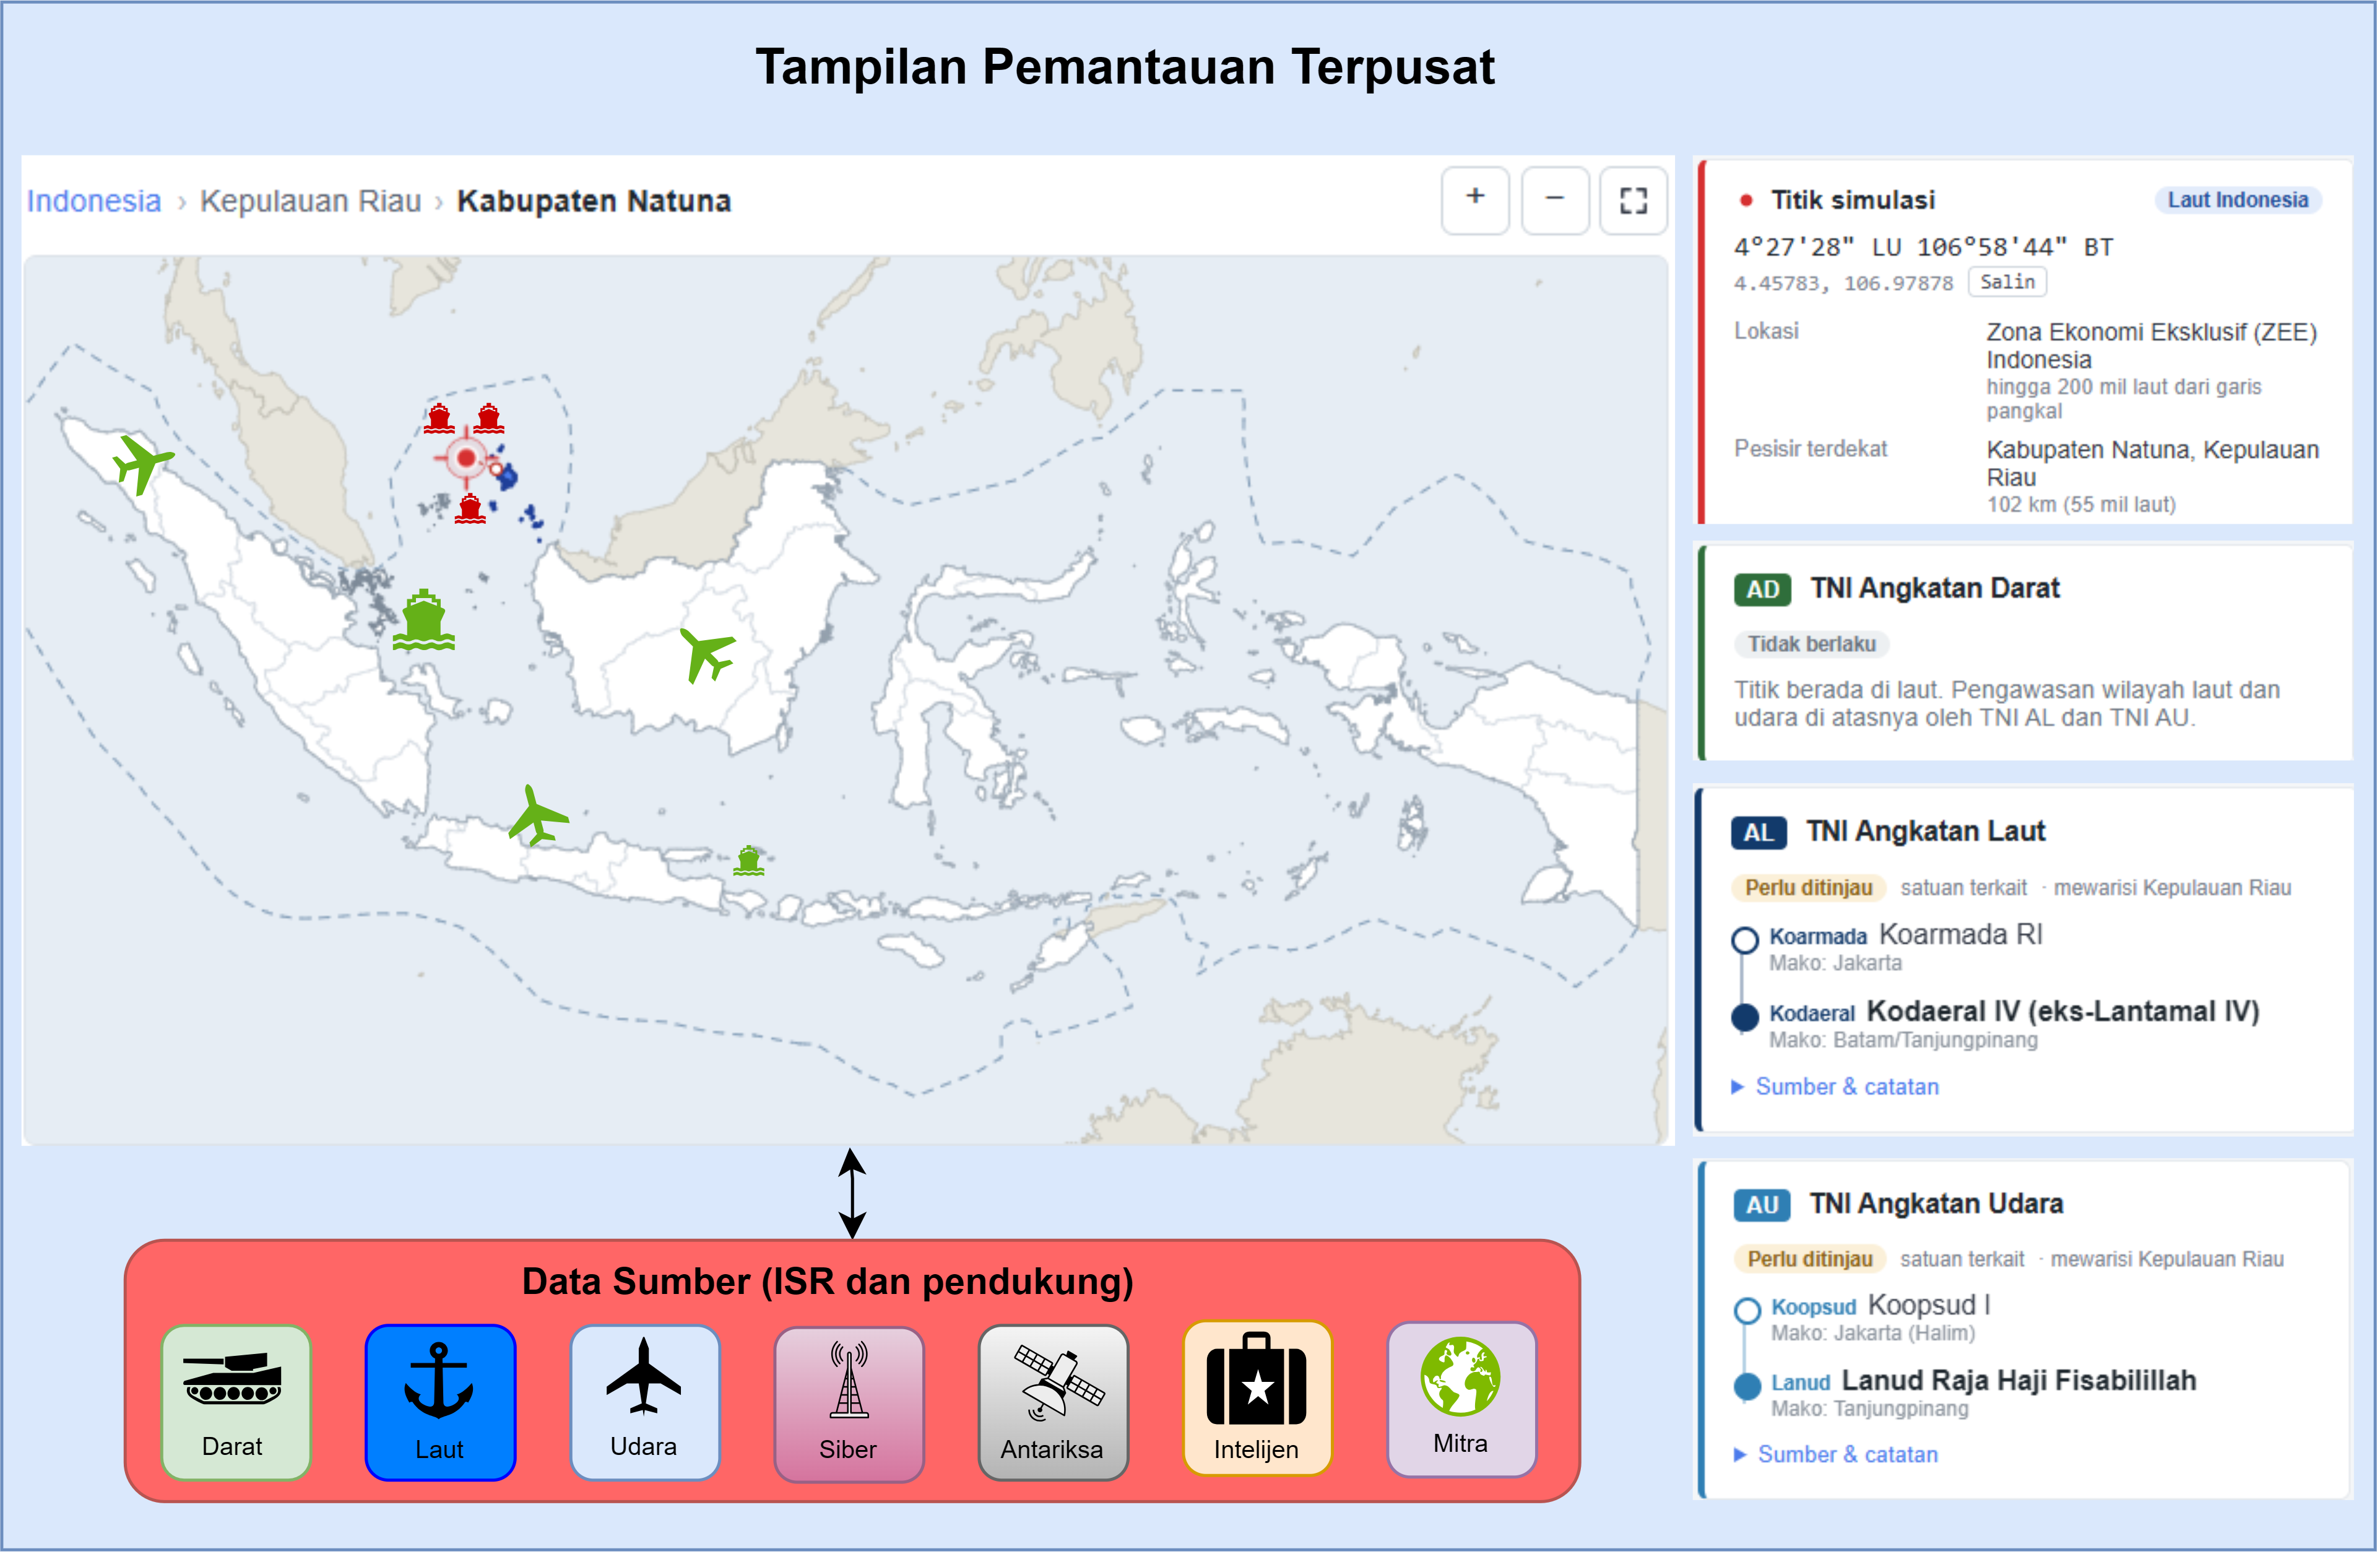
\includegraphics[width=0.99\linewidth,height=0.8\textheight,keepaspectratio]{images/Tampilan Pemantauan Terpusat.drawio.png}
\caption{Tampilan Pemantauan Terpusat}
\label{fig:IV.20}
\end{figure}

Gambar~\ref{fig:IV.20} menampilkan peta posisi unsur dan titik yang dipantau, panel informasi titik terpilih beserta satuan setiap matra yang terkait, serta data sumber ISR dari darat, laut, udara, siber, dan antariksa. Pada contoh titik simulasi di Zona Ekonomi Eksklusif sekitar Natuna, TNI AD ditandai tidak berlaku karena titik berada di laut, sedangkan TNI AL dan TNI AU menampilkan satuan terkait. Tampilan yang sama digunakan pada ketiga tingkat, dengan rincian yang dibatasi sesuai hak akses.

\subsubsection{\textit{Computers Layer}}
\label{sec:IV.6.4.2}

\textit{Computers Layer} mengolah data dari berbagai sumber menjadi informasi untuk pengambilan keputusan. Lapisan ini menggunakan komputasi terdistribusi pada tiga tingkat, sebagaimana ditunjukkan pada Gambar~\ref{fig:IV.21}.
\begin{figure}[htbp]
\centering
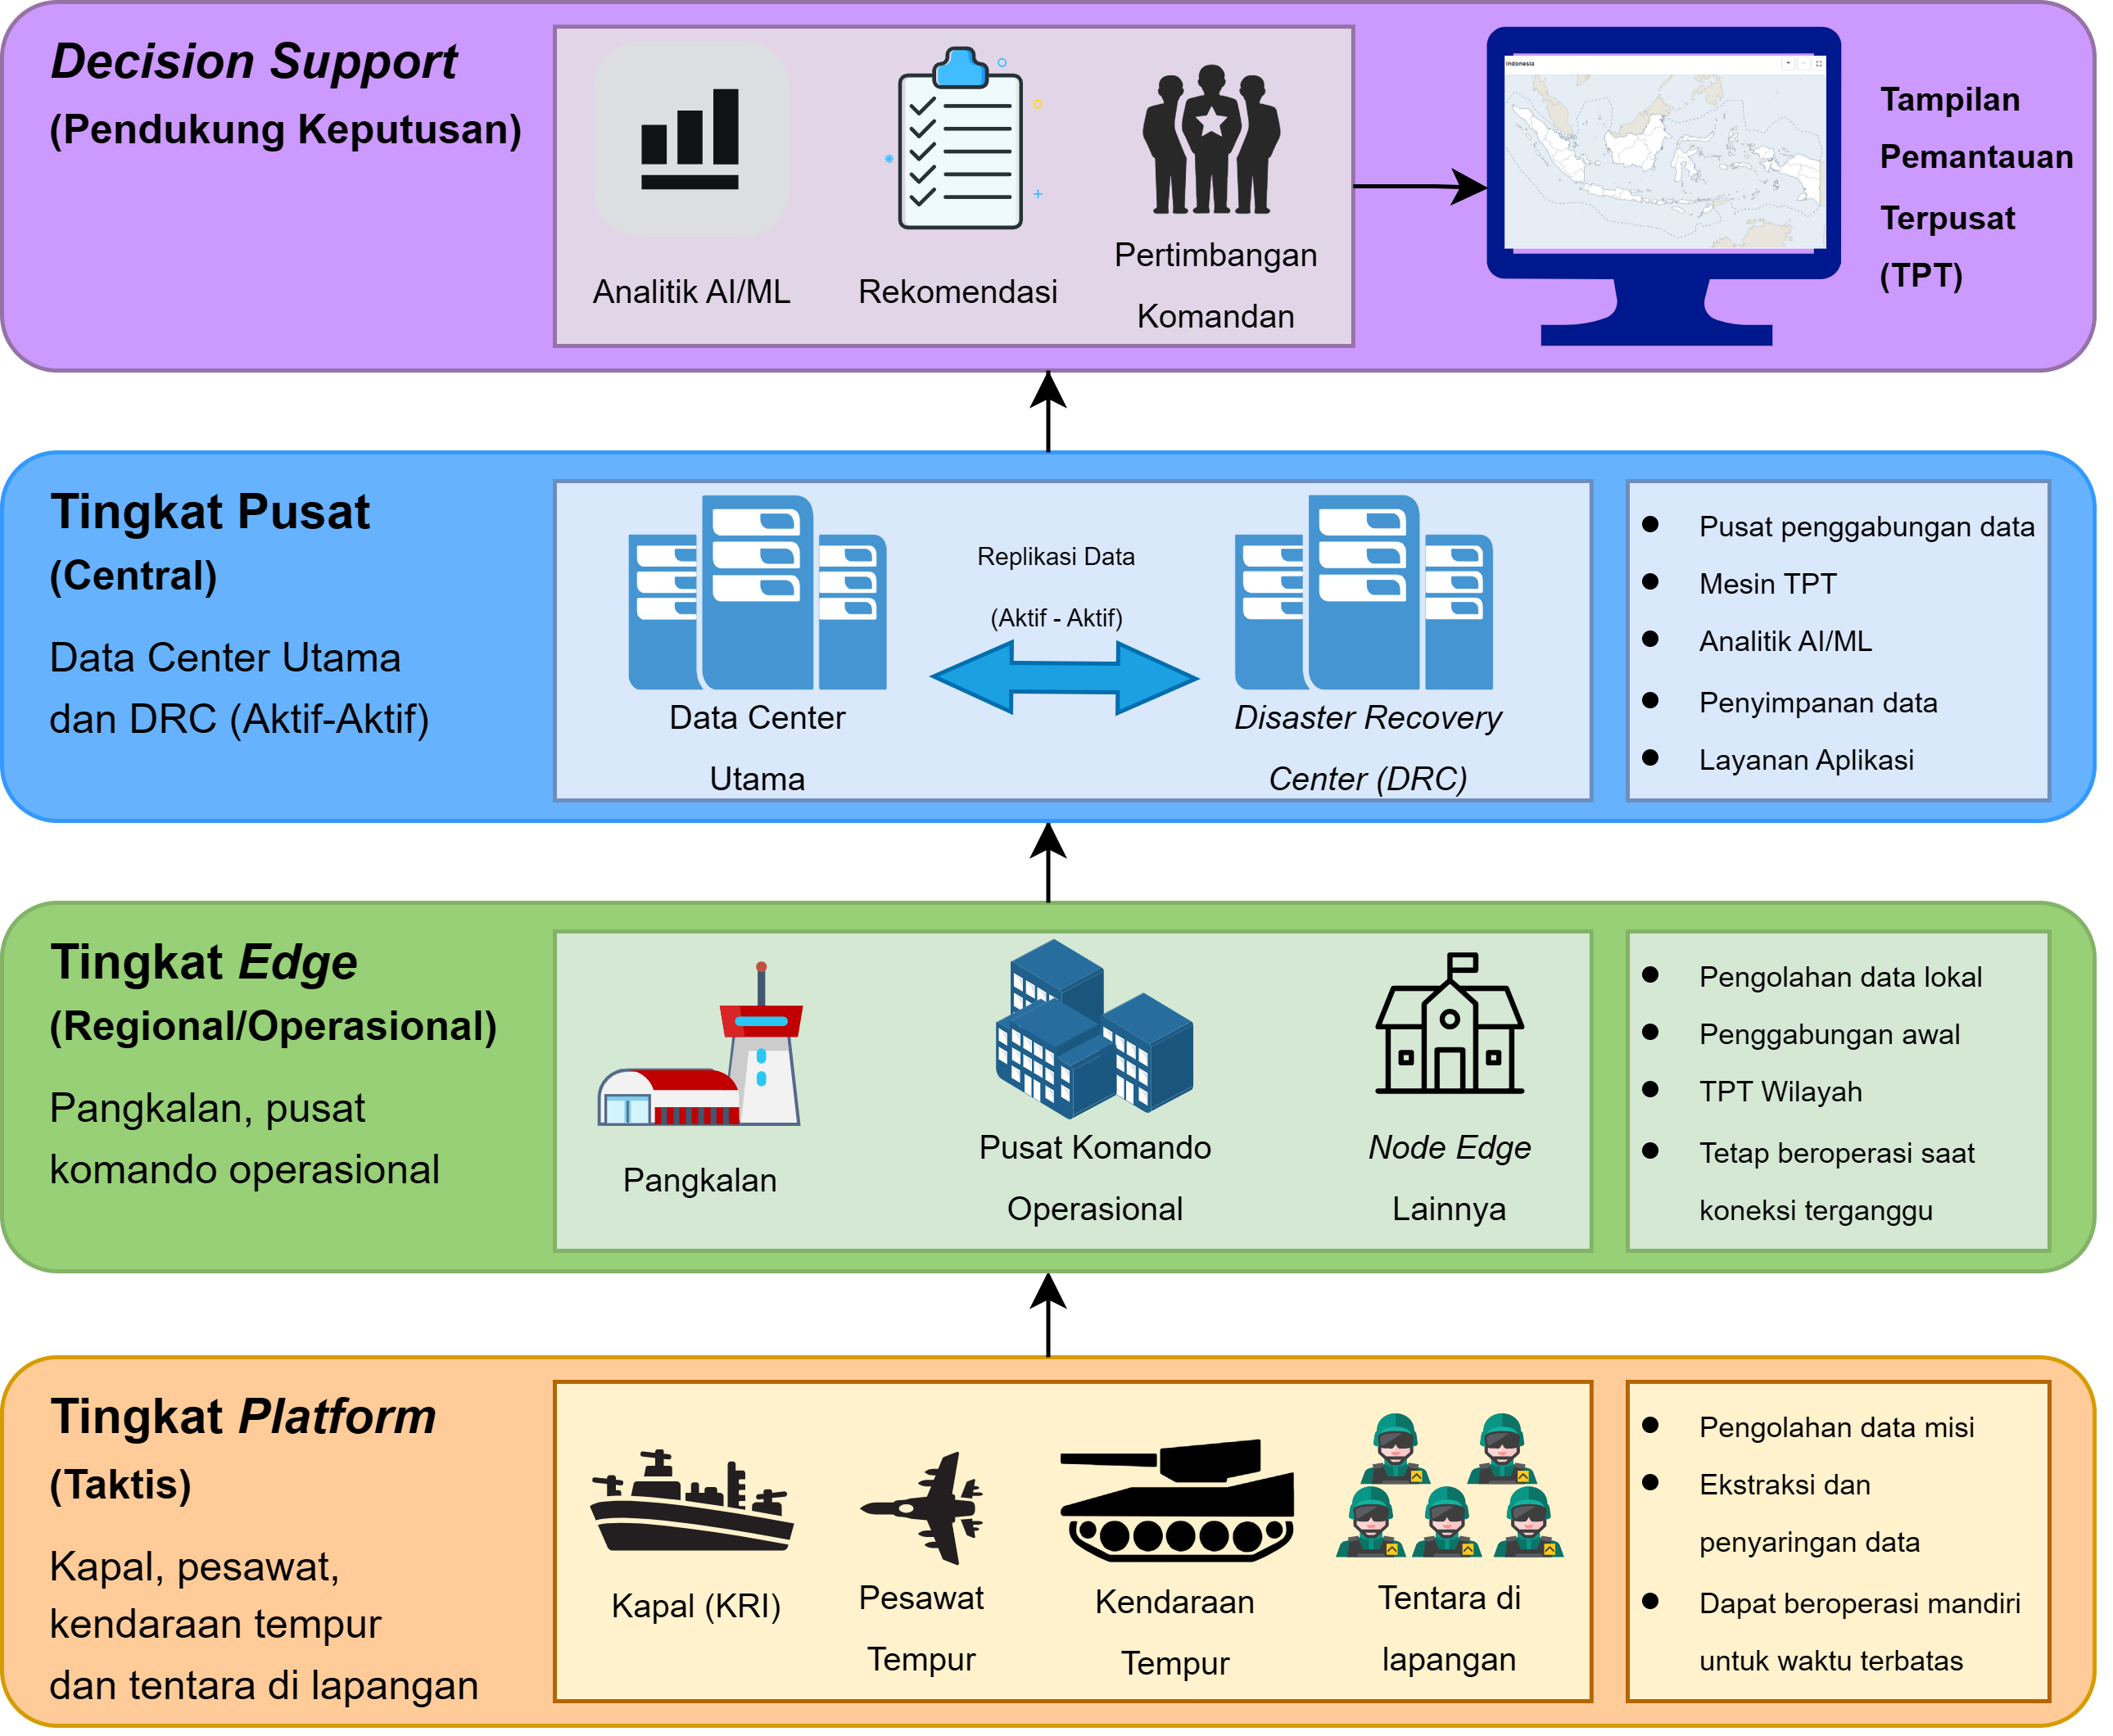
\includegraphics[width=0.99\linewidth,height=0.8\textheight,keepaspectratio]{images/Computers.drawio.png}
\caption{\textit{Computers Layer}}
\label{fig:IV.21}
\end{figure}

Gambar~\ref{fig:IV.21} menunjukkan bahwa data mengalir dari tingkat platform ke tingkat \textit{edge}, kemudian ke tingkat pusat. Tingkat platform berada pada kapal, pesawat, kendaraan tempur, dan satuan di lapangan untuk mengolah data misi, serta dapat beroperasi mandiri dalam waktu terbatas. Tingkat \textit{edge} berada di pangkalan dan pusat komando operasional untuk mengolah data lokal, menyediakan TPT wilayah, dan tetap beroperasi ketika koneksi ke pusat terganggu. Tingkat pusat berada pada \textit{Data Center} Utama dan DRC aktif-aktif untuk menjalankan penggabungan data seluruh matra, mesin TPT, penyimpanan data, dan analitik AI/ML.

Di atas ketiga tingkat terdapat fungsi \textit{decision support} yang memanfaatkan hasil penggabungan data dan analitik AI/ML untuk menghasilkan rekomendasi. Rekomendasi tersebut ditampilkan melalui TPT sebagai bahan pertimbangan, sedangkan keputusan akhir tetap berada pada komandan.

\subsubsection{\textit{Communications Layer}}
\label{sec:IV.6.4.3}

Wilayah Indonesia yang luas dan berbentuk kepulauan menuntut komunikasi C6ISR yang tidak bergantung pada satu media. Oleh karena itu, \textit{Communications Layer} menggunakan skema PACE (\textit{Primary, Alternate, Contingency, Emergency}) \cite{CISAPACE2023}, yaitu empat lapis jalur komunikasi dengan media berbeda sehingga gangguan pada satu jalur dapat dialihkan ke jalur lainnya. Skema tersebut ditunjukkan pada Gambar~\ref{fig:IV.22}.
\begin{figure}[htbp]
\centering
\includegraphics[width=0.93\linewidth,height=0.8\textheight,keepaspectratio]{images/Communication.drawio.png}
\caption{\textit{Communications Layer} dengan Skema PACE}
\label{fig:IV.22}
\end{figure}

Gambar~\ref{fig:IV.22} membedakan setiap lapis PACE berdasarkan warna jalur. Sarana dan peran setiap lapis dirangkum pada Tabel~\ref{tab:IV.26}.

\begingroup\small\setstretch{1.0}
\begin{longtable}{@{}>{\raggedright\arraybackslash\hspace{0pt}}p{0.161\linewidth}>{\raggedright\arraybackslash\hspace{0pt}}p{0.361\linewidth}>{\raggedright\arraybackslash\hspace{0pt}}p{0.415\linewidth}@{}}
\caption{Skema PACE Komunikasi C6ISR}\label{tab:IV.26}\\
\toprule
\textbf{Lapis} & \textbf{Sarana} & \textbf{Peran}\\
\midrule
\endfirsthead
\multicolumn{3}{@{}l}{\small\itshape \tablename\ \thetable{} (lanjutan)}\\
\toprule
\textbf{Lapis} & \textbf{Sarana} & \textbf{Peran}\\
\midrule
\endhead
\bottomrule
\endlastfoot
\textit{Primary} & Jaringan serat optik dan terestrial pertahanan & Jalur utama antarsimpul tetap, yaitu pusat komando, \textit{Data Center}, DRC, pangkalan, dan terminal SATCOM\\
\textit{Alternate} & SATCOM melalui sewa kapasitas atau satelit \textit{dual-use} nasional berpersandian & Komunikasi bagi wilayah terpencil, perbatasan, dan platform yang bergerak\\
\textit{Contingency} & \textit{Tactical data link} dan radio taktis V/UHF & Komunikasi langsung antarplatform taktis ketika jalur utama tidak tersedia\\
\textit{Emergency} & Radio HF jarak jauh dan \textit{airborne relay} (UAV/HAPS) & Komunikasi minimum ketika jalur lainnya terganggu\\
\end{longtable}
\endgroup

\subsubsection{\textit{Cyber Defense Layer}}
\label{sec:IV.6.4.4}

Berbeda dengan Subbab~\ref{sec:IV.5.4} yang melindungi infrastruktur teknologi, \textit{Cyber Defense Layer} difokuskan pada perlindungan operasi, data, komunikasi, dan sistem C6ISR. Lapisan ini menerapkan empat domain pelindungan pada Permenhan Nomor 34 Tahun 2025 \cite{Permenhan34Tahun2025} serta prinsip \textit{zero trust} \cite{NISTZeroTrust2020}, yaitu setiap pengguna, perangkat, dan koneksi harus diverifikasi sebelum diberi akses meskipun berada di dalam jaringan pertahanan. Kerangka \textit{cyber defense} C6ISR ditunjukkan pada Gambar~\ref{fig:IV.23}.
\begin{figure}[htbp]
\centering
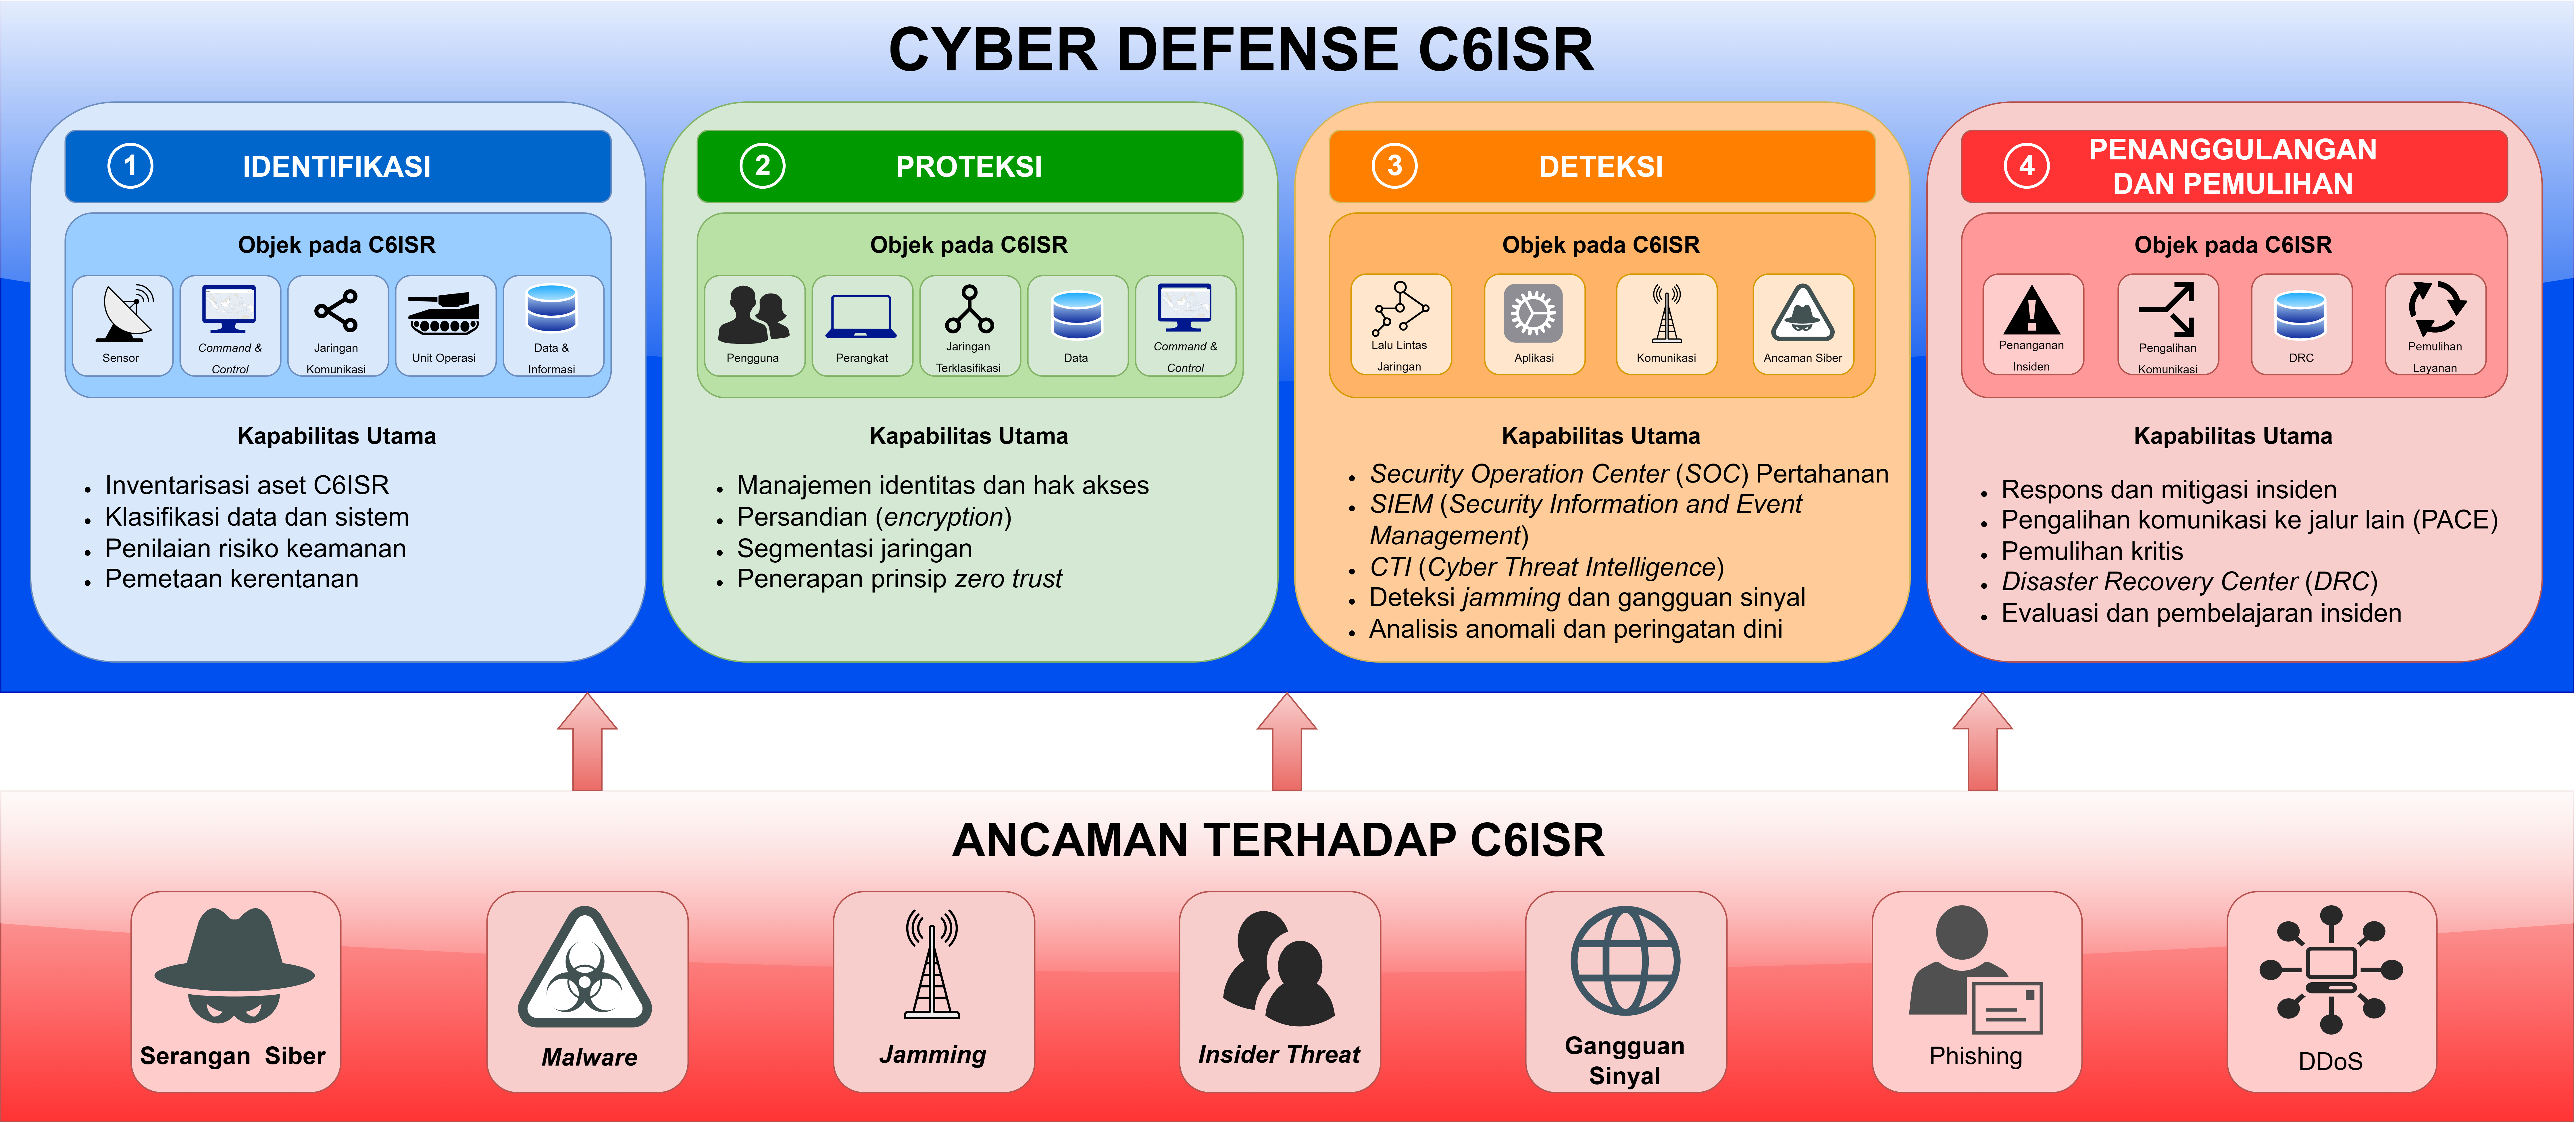
\includegraphics[width=0.99\linewidth,height=0.8\textheight,keepaspectratio]{images/Cyber Defense.drawio.png}
\caption{\textit{Cyber Defense} C6ISR}
\label{fig:IV.23}
\end{figure}

Gambar~\ref{fig:IV.23} menunjukkan bahwa keempat domain disusun untuk menghadapi ancaman terhadap C6ISR, yaitu serangan siber, \textit{malware}, \textit{jamming}, \textit{insider threat}, gangguan sinyal, \textit{phishing}, dan DDoS. Objek dan kapabilitas setiap domain dirinci pada Tabel~\ref{tab:IV.27}.

\begingroup\small\setstretch{1.0}
\begin{longtable}{@{}>{\raggedright\arraybackslash\hspace{0pt}}p{0.201\linewidth}>{\raggedright\arraybackslash\hspace{0pt}}p{0.321\linewidth}>{\raggedright\arraybackslash\hspace{0pt}}p{0.415\linewidth}@{}}
\caption{\textit{Cyber Defense} C6ISR}\label{tab:IV.27}\\
\toprule
\textbf{Domain} & \textbf{Objek pada C6ISR} & \textbf{Kapabilitas}\\
\midrule
\endfirsthead
\multicolumn{3}{@{}l}{\small\itshape \tablename\ \thetable{} (lanjutan)}\\
\toprule
\textbf{Domain} & \textbf{Objek pada C6ISR} & \textbf{Kapabilitas}\\
\midrule
\endhead
\bottomrule
\endlastfoot
Identifikasi & Sensor, platform, pusat komando, dan jaringan komunikasi & Inventarisasi aset, klasifikasi data, dan penilaian risiko keamanan\\
Proteksi & Pengguna, perangkat, jaringan terklasifikasi, dan data TPT & Manajemen identitas dan akses, persandian, segmentasi jaringan, \textit{Cross-Domain Gateway}, dan \textit{zero trust}\\
Deteksi & Lalu lintas jaringan, aplikasi \textit{Command \& Control}, dan spektrum komunikasi & SOC Pertahanan, SIEM, CTI, serta deteksi \textit{jamming} dan gangguan sinyal\\
Penanggulangan dan Pemulihan & Layanan dan sistem C6ISR yang kritis & Penanganan insiden, pengalihan jalur sesuai skema PACE, pemulihan melalui DRC, serta evaluasi pascainsiden\\
\end{longtable}
\endgroup

Tabel~\ref{tab:IV.27} menunjukkan bahwa \textit{cyber defense} pada C6ISR tidak hanya melindungi komputer dan jaringan, tetapi juga sensor, sistem komando-kendali, jalur komunikasi, dan platform operasional. Dengan demikian, \textit{cyber defense} melekat pada seluruh lapisan C6ISR, bukan sebagai komponen tambahan.

\subsubsection{\textit{Combat Systems Layer}}
\label{sec:IV.6.4.5}

Integrasi \textit{combat systems} merupakan pembeda utama C6ISR dari C5ISR. Integrasi tidak menuntut seluruh sistem tempur menggunakan perangkat yang sama, tetapi setiap sistem harus dapat bertukar informasi dengan \textit{Command \& Control} melalui antarmuka dan standar terbuka. Pendekatan arsitektur terbuka ini memungkinkan alutsista dari berbagai matra dan produsen bekerja dalam satu arsitektur serta mengurangi ketergantungan pada satu produsen. Hubungan \textit{Command \& Control}, \textit{combat systems}, dan ISR ditunjukkan pada Gambar~\ref{fig:IV.24}.
\begin{figure}[htbp]
\centering
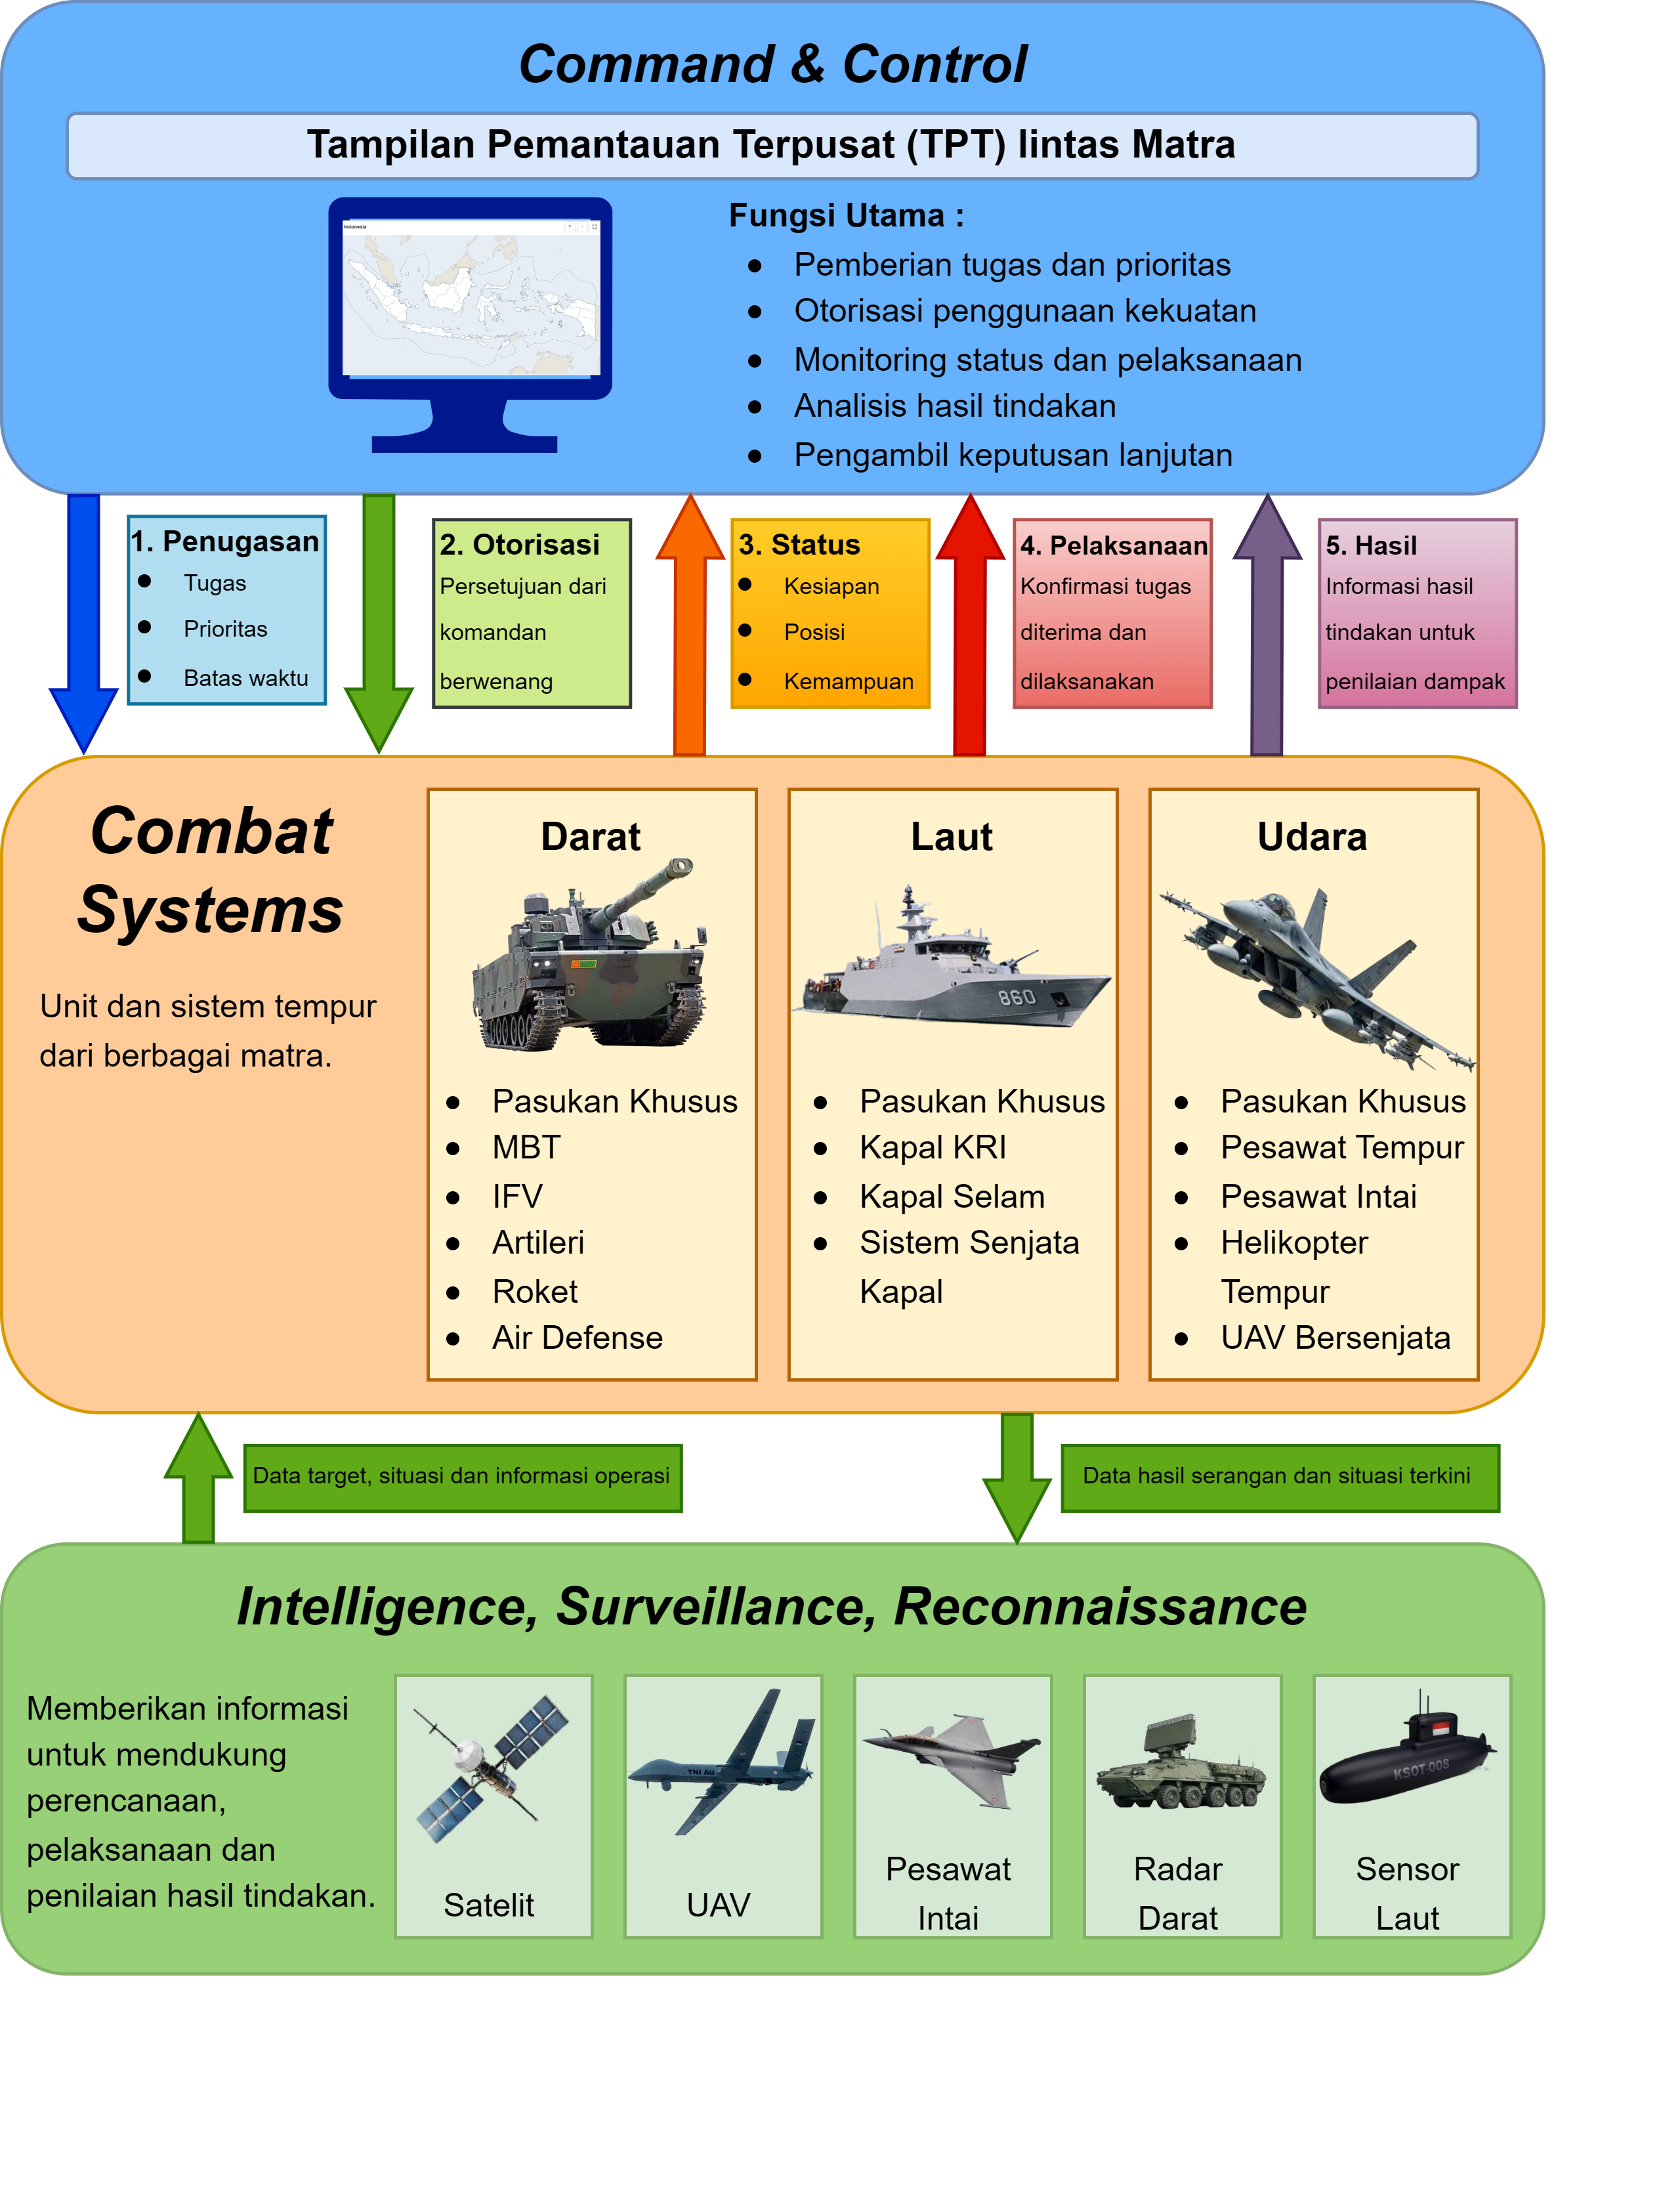
\includegraphics[width=0.82\linewidth,height=0.8\textheight,keepaspectratio]{images/Combat Systems.drawio.png}
\caption{\textit{Combat Systems} C6ISR}
\label{fig:IV.24}
\end{figure}

Gambar~\ref{fig:IV.24} menunjukkan bahwa ISR memberikan data sasaran dan situasi kepada \textit{combat systems} serta menerima data hasil tindakan untuk penilaian. Di antara \textit{Command \& Control} dan \textit{combat systems} terdapat lima aliran informasi yang dirinci pada Tabel~\ref{tab:IV.28}.

\begingroup\small\setstretch{1.0}
\begin{longtable}{@{}>{\raggedright\arraybackslash\hspace{0pt}}p{0.168\linewidth}>{\raggedright\arraybackslash\hspace{0pt}}p{0.194\linewidth}>{\raggedright\arraybackslash\hspace{0pt}}p{0.194\linewidth}>{\raggedright\arraybackslash\hspace{0pt}}p{0.350\linewidth}@{}}
\caption{Aliran Informasi \textit{Combat Systems}}\label{tab:IV.28}\\
\toprule
\textbf{Aliran} & \textbf{Dari} & \textbf{Ke} & \textbf{Isi Informasi}\\
\midrule
\endfirsthead
\multicolumn{4}{@{}l}{\small\itshape \tablename\ \thetable{} (lanjutan)}\\
\toprule
\textbf{Aliran} & \textbf{Dari} & \textbf{Ke} & \textbf{Isi Informasi}\\
\midrule
\endhead
\bottomrule
\endlastfoot
Penugasan & \textit{Command \& Control} & \textit{Combat Systems} & Tugas, prioritas, wilayah operasi, dan batas waktu\\
Otorisasi & Komandan berwenang & \textit{Combat Systems} & Persetujuan tindakan sesuai aturan pelibatan\\
Status kesiapan & \textit{Combat Systems} & \textit{Command \& Control} & Kesiapan, posisi, dan kemampuan platform\\
Pelaksanaan & \textit{Combat Systems} & \textit{Command \& Control} & Konfirmasi bahwa tugas telah diterima dan dilaksanakan\\
Hasil tindakan & \textit{Combat Systems} dan ISR & \textit{Intelligence} dan \textit{Command \& Control} & Hasil tindakan untuk penilaian dampak (\textit{battle damage assessment}) dan penentuan langkah berikutnya\\
\end{longtable}
\endgroup

Tabel~\ref{tab:IV.28} menunjukkan bahwa aliran otorisasi selalu berasal dari komandan berwenang. Dengan demikian, integrasi \textit{combat systems} tidak menghilangkan peran manusia. Sistem membantu menyampaikan informasi dan melaksanakan tugas, tetapi keputusan penggunaan kekuatan tetap berada pada komandan, sejalan dengan prinsip pertimbangan manusia dalam penggunaan kekuatan \cite{DoDD300009}.

\subsubsection{\textit{ISR Layer}}
\label{sec:IV.6.4.6}

\textit{ISR Layer} menggabungkan data dari berbagai sensor menjadi informasi yang utuh mengenai kondisi lapangan. Alur integrasinya ditunjukkan pada Gambar~\ref{fig:IV.25}.
\begin{figure}[htbp]
\centering
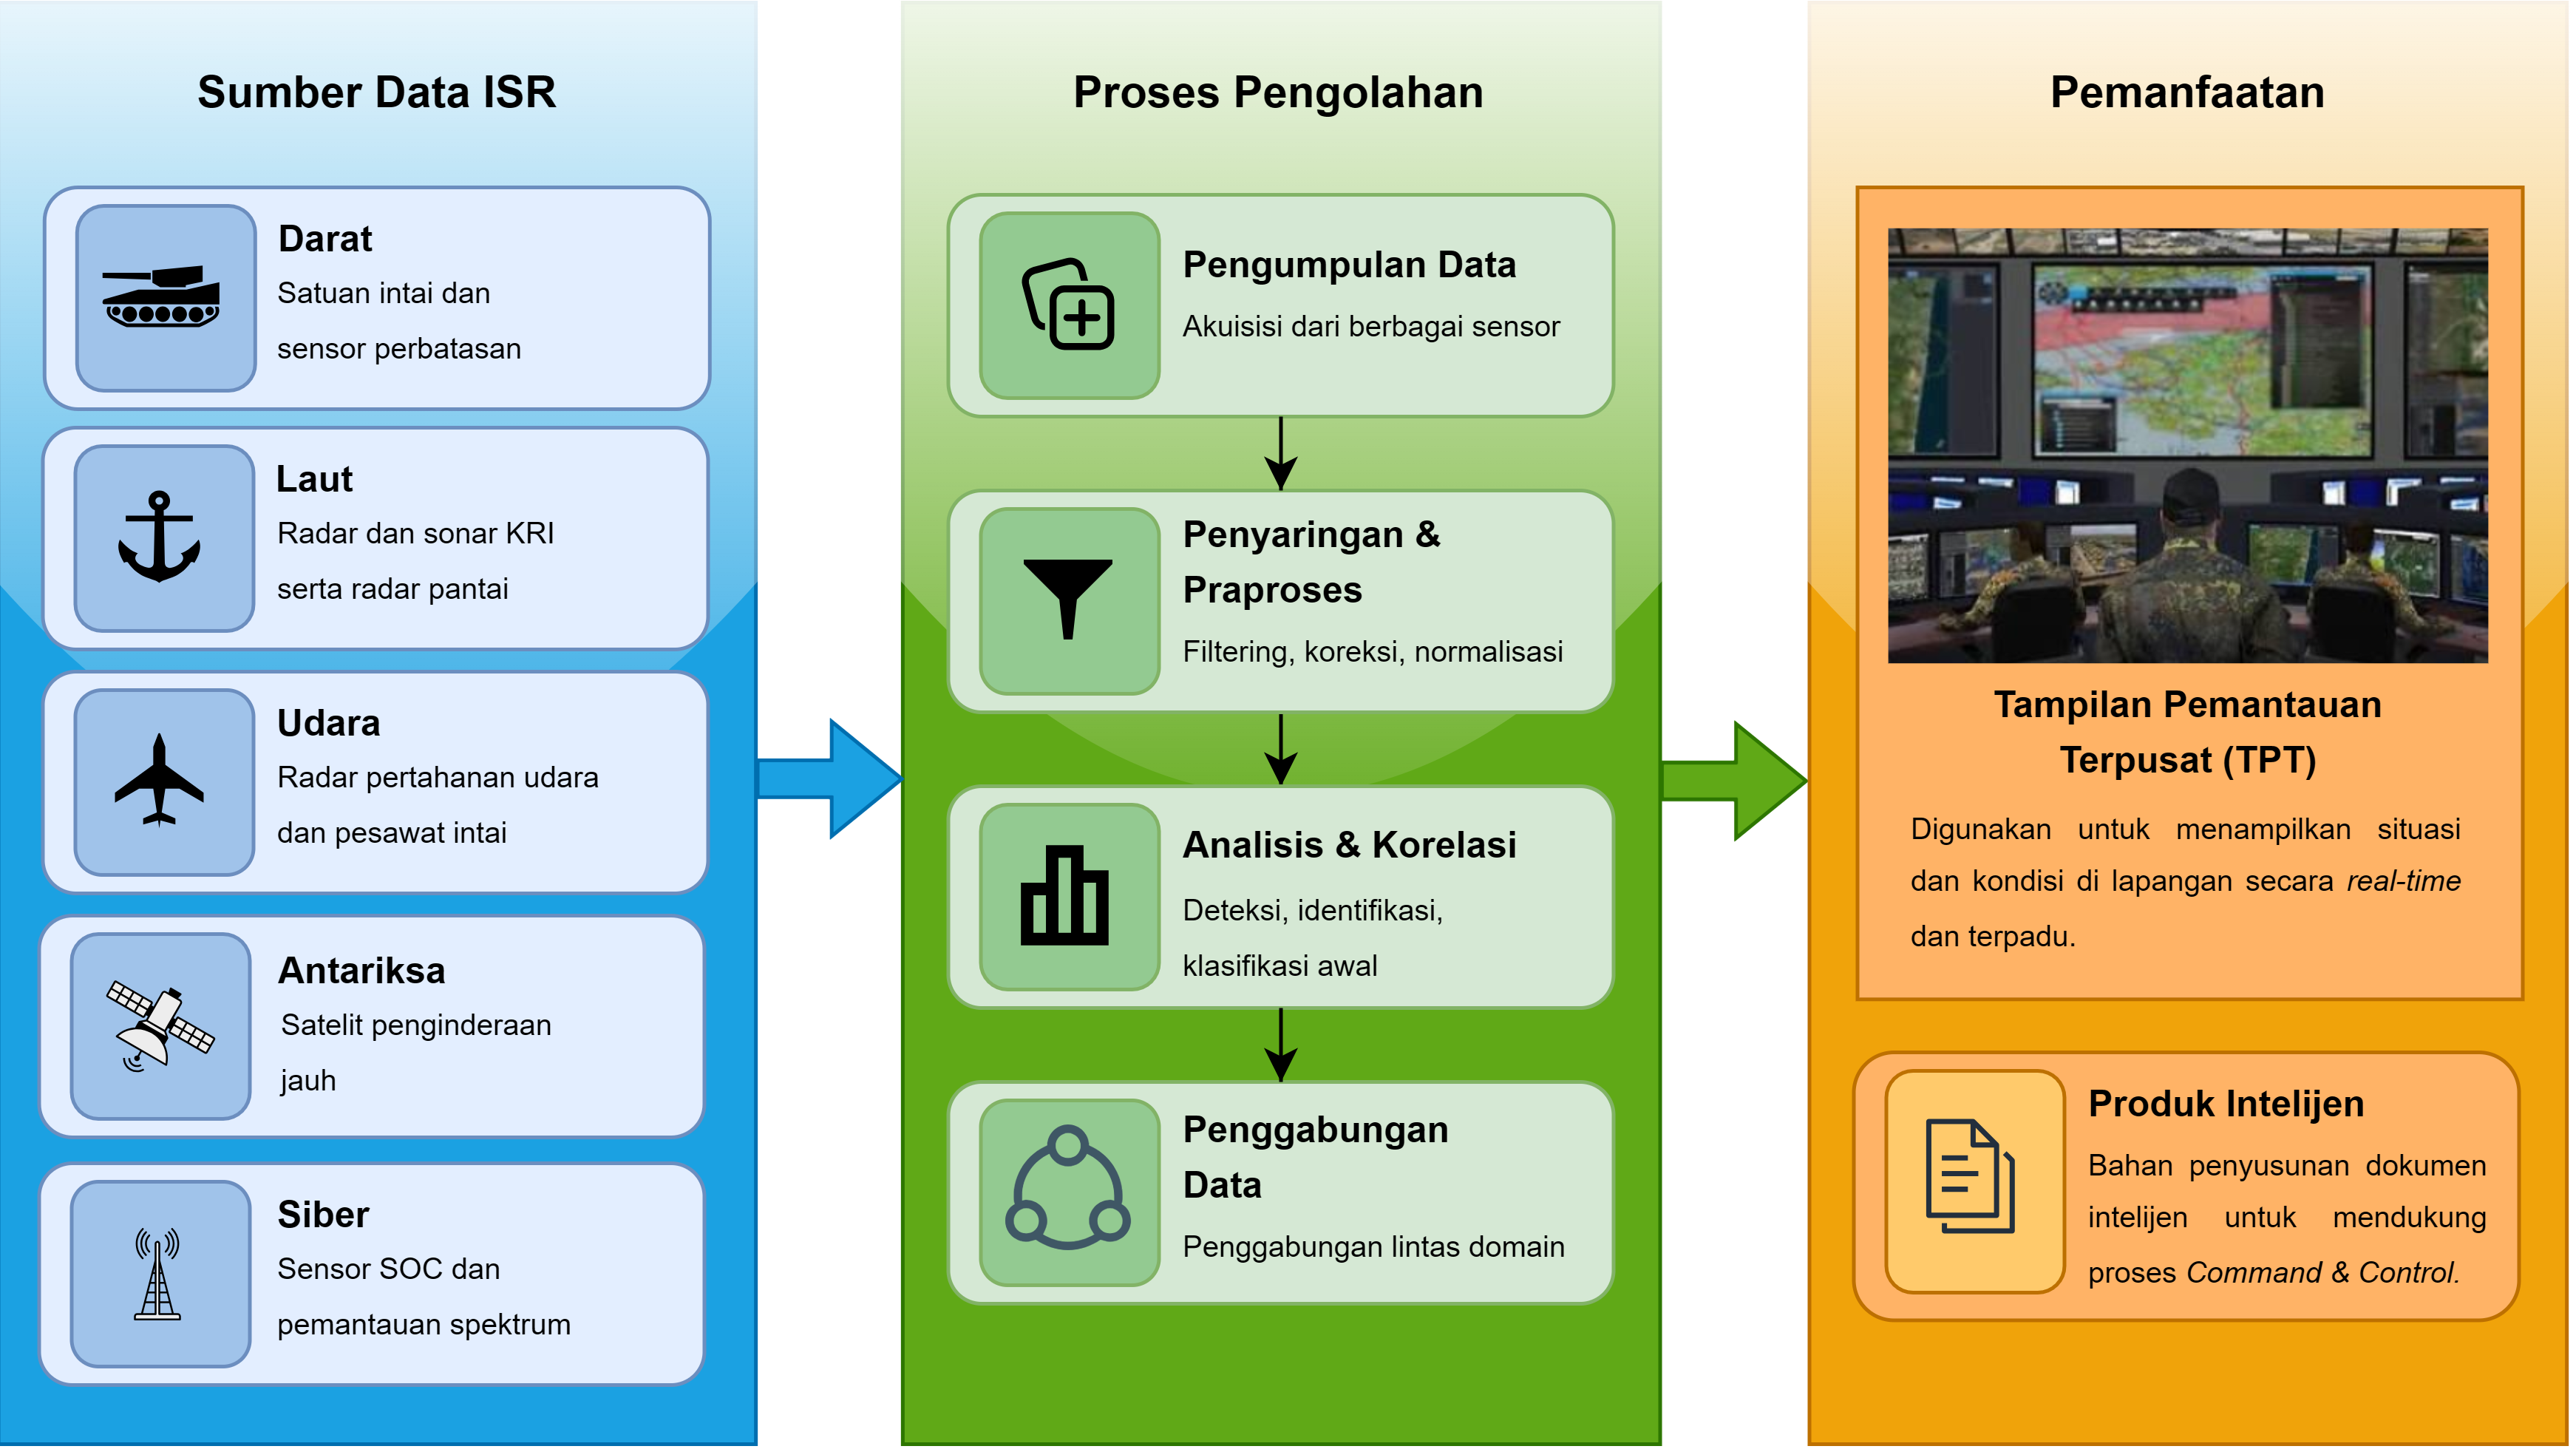
\includegraphics[width=0.99\linewidth,height=0.8\textheight,keepaspectratio]{images/ISR.drawio.png}
\caption{\textit{ISR Layer}}
\label{fig:IV.25}
\end{figure}

Gambar~\ref{fig:IV.25} menunjukkan bahwa data dari lima domain, yaitu darat, laut, udara, antariksa, dan siber, diolah melalui empat tahap, yaitu pengumpulan, penyaringan dan praproses, analisis dan korelasi, serta penggabungan lintas domain. Hasilnya dimanfaatkan sebagai TPT \textit{real-time} dan bahan produk intelijen untuk mendukung \textit{Command \& Control}. Rincian setiap domain disajikan pada Tabel~\ref{tab:IV.29}.

\begingroup\small\setstretch{1.0}
\begin{longtable}{@{}>{\raggedright\arraybackslash\hspace{0pt}}p{0.168\linewidth}>{\raggedright\arraybackslash\hspace{0pt}}p{0.246\linewidth}>{\raggedright\arraybackslash\hspace{0pt}}p{0.227\linewidth}>{\raggedright\arraybackslash\hspace{0pt}}p{0.266\linewidth}@{}}
\caption{Sumber dan Aliran Data ISR}\label{tab:IV.29}\\
\toprule
\textbf{Domain} & \textbf{Sumber Sensor} & \textbf{Data yang Dihasilkan} & \textbf{Pengolahan}\\
\midrule
\endfirsthead
\multicolumn{4}{@{}l}{\small\itshape \tablename\ \thetable{} (lanjutan)}\\
\toprule
\textbf{Domain} & \textbf{Sumber Sensor} & \textbf{Data yang Dihasilkan} & \textbf{Pengolahan}\\
\midrule
\endhead
\bottomrule
\endlastfoot
\centering\arraybackslash Udara & Radar pertahanan udara dan pesawat intai & Jejak (\textit{track}) sasaran udara & Digabungkan dan dibandingkan dengan data penerbangan sipil\\
\centering\arraybackslash Laut & Radar dan sonar KRI serta radar pantai & Jejak kapal dan kontak bawah air & Digabungkan dan dibandingkan dengan informasi identitas kapal\\
\centering\arraybackslash Darat & Satuan intai dan sensor perbatasan & Laporan pengamatan dan citra & Diperiksa dan dianalisis oleh analis intelijen\\
\centering\arraybackslash Antariksa & Satelit penginderaan jauh & Citra wilayah & Dianalisis untuk memperoleh informasi kondisi wilayah\\
\centering\arraybackslash Siber dan spektrum & Sensor SOC dan pemantauan spektrum & Peringatan serangan siber dan gangguan sinyal & Dianalisis dan dikorelasikan di SOC Pertahanan\\
\end{longtable}
\endgroup

Tabel~\ref{tab:IV.29} menunjukkan bahwa setiap domain menghasilkan data dengan bentuk berbeda. Oleh karena itu, setiap data hasil penggabungan dilengkapi metadata, seperti sumber, waktu pengambilan, tingkat keyakinan, dan klasifikasi, agar dapat dipertukarkan antarmatra tanpa kehilangan konteksnya.

\subsection{Analisis Kesenjangan}
\label{sec:IV.6.5}

Analisis kesenjangan dilakukan per lapisan C6ISR. Setiap kesenjangan ditautkan dengan kode kebutuhan operasional pada Tabel~\ref{tab:IV.23} agar tindak lanjutnya tetap berpijak pada kebutuhan pertahanan. Hasilnya disajikan pada Tabel~\ref{tab:IV.30}.

\begingroup\small\setstretch{1.0}
\begin{longtable}{@{}>{\raggedright\arraybackslash\hspace{0pt}}p{0.060\linewidth}>{\raggedright\arraybackslash\hspace{0pt}}p{0.164\linewidth}>{\raggedright\arraybackslash\hspace{0pt}}p{0.173\linewidth}>{\raggedright\arraybackslash\hspace{0pt}}p{0.173\linewidth}>{\raggedright\arraybackslash\hspace{0pt}}p{0.198\linewidth}>{\raggedright\arraybackslash\hspace{0pt}}p{0.078\linewidth}@{}}
\caption{Analisis Kesenjangan Arsitektur C6ISR}\label{tab:IV.30}\\
\toprule
\textbf{No.} & \textbf{Lapisan} & \textbf{Kondisi \textit{Baseline}} & \textbf{Kondisi Target} & \textbf{Tindak Lanjut} & \textbf{KO}\\
\midrule
\endfirsthead
\multicolumn{6}{@{}l}{\small\itshape \tablename\ \thetable{} (lanjutan)}\\
\toprule
\textbf{No.} & \textbf{Lapisan} & \textbf{Kondisi \textit{Baseline}} & \textbf{Kondisi Target} & \textbf{Tindak Lanjut} & \textbf{KO}\\
\midrule
\endhead
\bottomrule
\endlastfoot
\centering\arraybackslash 1 & \textit{Command \& Control} & Dikembangkan per matra; belum ada aplikasi lintas matra dan gambaran situasi bersama & Berjenjang tiga tingkat dengan TPT lintas matra dan \textit{mission command} & Pengembangan TPT dan aplikasi \textit{Command \& Control} lintas matra; penetapan prosedur berjenjang dan hak akses per tingkat & \centering\arraybackslash KO-01\newline KO-03\\
\centering\arraybackslash 2 & \textit{Computers} & Satu \textit{Data Center} tanpa DRC; belum ada fusi data dan analitik operasional & Komputasi pusat, \textit{edge}, dan platform dengan fusi data, mesin TPT, AI/ML, dan \textit{decision support} & Pembangunan pusat fusi data dan mesin TPT; penyediaan \textit{edge computing}; pengembangan analitik AI/ML dan \textit{decision support} & \centering\arraybackslash KO-03\newline KO-07\\
\centering\arraybackslash 3 & \textit{Communications} & Belum memiliki satelit pertahanan; jaringan belum lintas matra & Skema PACE dengan SATCOM berpersandian & Penerapan skema PACE; sewa SATCOM atau satelit \textit{dual-use} berpersandian; kajian satelit pertahanan nasional & \centering\arraybackslash KO-04\newline KO-05\\
\centering\arraybackslash 4 & \textit{Cyber Defense} & Parsial (kematangan level 1–2); belum ada jaringan operasional terklasifikasi & SOC Pertahanan, persandian, \textit{zero trust}, dan deteksi \textit{jamming}; kematangan level 3 pada 2029 & Pembangunan SOC Pertahanan dan jaringan terklasifikasi; penerapan \textit{zero trust} dan persandian; penguatan deteksi \textit{jamming} & \centering\arraybackslash KO-04\newline KO-06\newline KO-07\\
\centering\arraybackslash 5 & \textit{Combat Systems} & Standar antarmuka alutsista beragam; integrasi dengan \textit{Command \& Control} terbatas & Integrasi melalui antarmuka dan standar terbuka dengan lima aliran informasi & Penetapan standar antarmuka dan format data terbuka; integrasi alutsista eksisting melalui adaptor; standar interoperabilitas sebagai persyaratan pengadaan & \centering\arraybackslash KO-02\\
\centering\arraybackslash 6 & ISR & Sensor dikelola per matra; data belum difusikan; belum ada satelit ISR & Integrasi ISR lima domain dengan metadata sebagai sumber TPT & Integrasi aliran data sensor lintas matra; penetapan standar metadata ISR; pemanfaatan citra satelit dan pengembangan satelit ISR & \centering\arraybackslash KO-01\\
\end{longtable}
\endgroup

Tabel~\ref{tab:IV.30} menunjukkan bahwa kesenjangan C6ISR mengerucut pada tiga persoalan. Pertama, belum terbentuknya gambaran situasi bersama lintas matra pada lapisan \textit{Command \& Control}, \textit{Computers}, dan ISR. Kedua, ketergantungan komunikasi satelit pada pihak lain. Ketiga, keragaman antarmuka \textit{combat systems}.

\subsection{\textit{Roadmap}}
\label{sec:IV.6.6}

\textit{Roadmap} Fase C6ISR Architecture menyusun inisiatif berdasarkan ketergantungan antarkesenjangan pada Tabel~\ref{tab:IV.30}, sebagaimana disajikan pada Gambar~\ref{fig:IV.26}.
\begin{figure}[htbp]
\centering
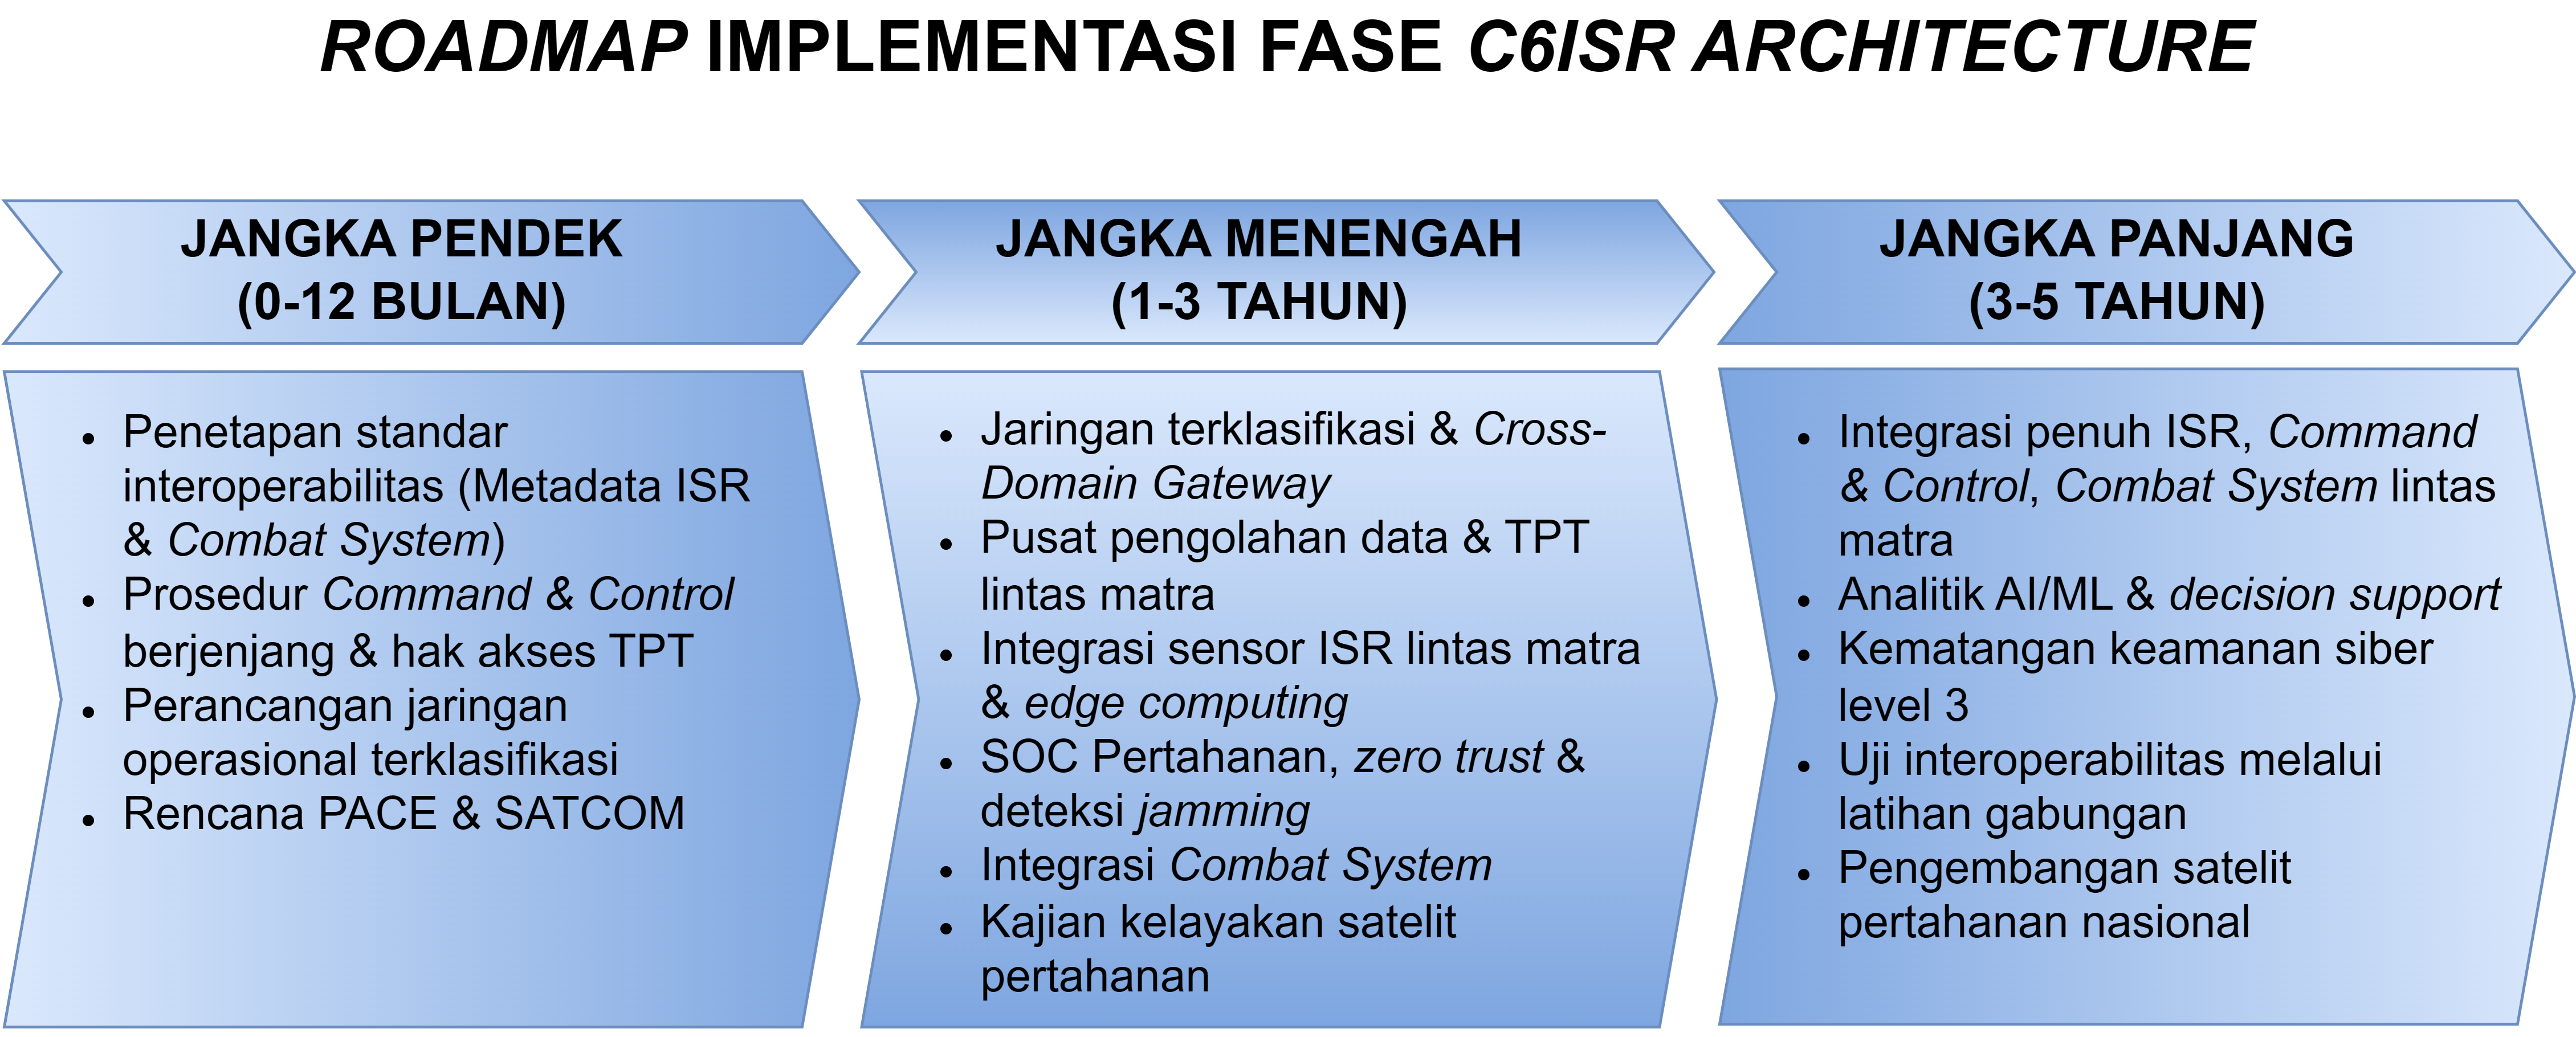
\includegraphics[width=0.99\linewidth,height=0.8\textheight,keepaspectratio]{images/Roadmap implementasi fase C6ISR Architecture.drawio.png}
\caption{\textit{Roadmap} Implementasi Fase C6ISR Architecture}
\label{fig:IV.26}
\end{figure}

Gambar~\ref{fig:IV.26} menunjukkan bahwa jangka pendek (0–12 bulan) difokuskan pada penetapan standar, prosedur, dan rancangan yang belum memerlukan infrastruktur besar, yaitu standar interoperabilitas \textit{combat systems} dan metadata ISR, prosedur \textit{Command \& Control} berjenjang dan hak akses TPT, rancangan jaringan operasional terklasifikasi, serta rencana PACE dan pemenuhan SATCOM. Jangka menengah (1–3 tahun) mewujudkan fondasi tersebut melalui jaringan terklasifikasi dan \textit{Cross-Domain Gateway}, pusat pengolahan data dan TPT lintas matra, integrasi sensor ISR dan \textit{edge computing}, SOC Pertahanan, serta integrasi \textit{combat systems} prioritas, disertai kajian kelayakan satelit pertahanan. Jangka panjang (3–5 tahun) memadukan ISR, \textit{Command \& Control}, dan \textit{combat systems} lintas matra secara penuh, memanfaatkan analitik AI/ML dan \textit{decision support}, mencapai kematangan keamanan siber level 3, menguji interoperabilitas melalui latihan gabungan, serta mengembangkan satelit pertahanan nasional.

Dengan demikian, Fase \textit{C6ISR Architecture} menghasilkan arsitektur C6ISR target yang memadukan unsur pengindraan, komando-kendali, dan unsur penindak lintas matra, dengan keputusan penggunaan kekuatan tetap berada pada komandan.

\section{Fase Opportunities \& Solutions}
\label{sec:IV.7}

Fase Opportunities \& Solutions menerjemahkan hasil Fase \textit{Business, Information Systems, Technology,} dan \textit{C6ISR Architecture} menjadi rencana pelaksanaan. Fase ini mengelompokkan kesenjangan ke dalam paket pekerjaan (\textit{work packages}), menetapkan urutan pelaksanaan berdasarkan ketergantungan, serta merumuskan arsitektur transisi dan \textit{roadmap} arsitektur.

\subsection{Atribut Perubahan dan Kendala}
\label{sec:IV.7.1}

Atribut perubahan menggambarkan pergeseran kondisi yang ingin dicapai melalui transformasi. Atribut tersebut dirangkum dari kondisi \textit{baseline} dan target setiap fase, sebagaimana disajikan pada Tabel~\ref{tab:IV.31}.

\begingroup\small\setstretch{1.0}
\begin{longtable}{@{}>{\raggedright\arraybackslash\hspace{0pt}}p{0.214\linewidth}>{\raggedright\arraybackslash\hspace{0pt}}p{0.348\linewidth}>{\raggedright\arraybackslash\hspace{0pt}}p{0.375\linewidth}@{}}
\caption{Atribut Perubahan Utama}\label{tab:IV.31}\\
\toprule
\textbf{Atribut} & \textbf{Kondisi Saat Ini} & \textbf{Arah Perubahan}\\
\midrule
\endfirsthead
\multicolumn{3}{@{}l}{\small\itshape \tablename\ \thetable{} (lanjutan)}\\
\toprule
\textbf{Atribut} & \textbf{Kondisi Saat Ini} & \textbf{Arah Perubahan}\\
\midrule
\endhead
\bottomrule
\endlastfoot
Tata kelola transformasi & Berjalan parsial tanpa mandat lintas organisasi & Terorkestrasi oleh DTO dan \textit{Architecture Board}\\
Data & Terkotak per aplikasi dan satuan kerja & Satu Data Pertahanan yang terstandar dan terklasifikasi\\
Aplikasi & 71 aplikasi khusus bersifat \textit{silo} dan sebagian berfungsi serupa & Aplikasi terkonsolidasi dan terintegrasi\\
Infrastruktur & Satu \textit{Data Center} tanpa DRC & \textit{Data Center} Utama dan DRC aktif-aktif\\
Keamanan siber & Parsial dengan kematangan level 1–2 & Menyeluruh dengan kematangan level 3 pada tahun 2029\\
C6ISR & \textit{Command \& Control} dikembangkan per matra & C6ISR terintegrasi lintas matra melalui TPT\\
\end{longtable}
\endgroup

Tabel~\ref{tab:IV.31} menunjukkan bahwa perubahan terjadi serentak pada enam atribut, mulai dari tata kelola hingga operasi pertahanan. Oleh karena itu, transformasi perlu ditahapkan dengan memperhatikan kendala implementasi pada Tabel~\ref{tab:IV.32}.

\begingroup\small\setstretch{1.0}
\begin{longtable}{@{}>{\raggedright\arraybackslash\hspace{0pt}}p{0.311\linewidth}>{\raggedright\arraybackslash\hspace{0pt}}p{0.656\linewidth}@{}}
\caption{Kendala Implementasi dan Implikasinya}\label{tab:IV.32}\\
\toprule
\textbf{Kendala} & \textbf{Implikasi}\\
\midrule
\endfirsthead
\multicolumn{2}{@{}l}{\small\itshape \tablename\ \thetable{} (lanjutan)}\\
\toprule
\textbf{Kendala} & \textbf{Implikasi}\\
\midrule
\endhead
\bottomrule
\endlastfoot
Keterbatasan SDM digital & Pengembangan talenta digital berjalan paralel dengan paket teknis; pelaksanaan awal memanfaatkan unit yang telah ada\\
Keberadaan sistem lama (\textit{legacy}) & Integrasi dilakukan bertahap melalui API dan standar terbuka, bukan penggantian sistem sekaligus\\
Kerahasiaan dan keamanan pertahanan & Data Rahasia baru dialirkan setelah jaringan operasional terklasifikasi tersedia\\
Keterbatasan anggaran dan waktu & Jangka pendek difokuskan pada inisiatif fondasi berbiaya rendah, seperti standar dan regulasi; investasi besar ditempatkan pada jangka menengah dan panjang\\
\end{longtable}
\endgroup

Tabel~\ref{tab:IV.32} menunjukkan bahwa setiap kendala membatasi susunan paket pekerjaan dan urutan pelaksanaannya.

\subsection{Konsolidasi Kesenjangan}
\label{sec:IV.7.2}

Kesenjangan dari Fase \textit{Business} hingga Fase \textit{C6ISR Architecture} disatukan agar inisiatif yang beririsan tidak dilaksanakan berulang. Hasil konsolidasi disajikan pada Tabel~\ref{tab:IV.33}. Kolom asal kesenjangan memuat nomor tabel analisis kesenjangan beserta nomor barisnya.

\begingroup\small\setstretch{1.0}
\begin{longtable}{@{}>{\raggedright\arraybackslash\hspace{0pt}}p{0.065\linewidth}>{\raggedright\arraybackslash\hspace{0pt}}p{0.233\linewidth}>{\raggedright\arraybackslash\hspace{0pt}}p{0.421\linewidth}>{\raggedright\arraybackslash\hspace{0pt}}p{0.188\linewidth}@{}}
\caption{Konsolidasi Kesenjangan}\label{tab:IV.33}\\
\toprule
\textbf{No.} & \textbf{Kelompok Kesenjangan} & \textbf{Inti Persoalan} & \textbf{Asal Kesenjangan}\\
\midrule
\endfirsthead
\multicolumn{4}{@{}l}{\small\itshape \tablename\ \thetable{} (lanjutan)}\\
\toprule
\textbf{No.} & \textbf{Kelompok Kesenjangan} & \textbf{Inti Persoalan} & \textbf{Asal Kesenjangan}\\
\midrule
\endhead
\bottomrule
\endlastfoot
\centering\arraybackslash 1 & Tata kelola dan mandat transformasi & Belum ada fungsi yang mengorkestrasi transformasi serta tata kelola arsitektur, data, dan portofolio aplikasi & Tabel IV.11 (1, 2)\newline Tabel IV.16 (3)\newline Tabel IV.19 (5)\\
\centering\arraybackslash 2 & Proses bisnis, manajemen perubahan, dan talenta digital & Proses terfragmentasi, perubahan tidak dikelola, koordinasi lintas matra \textit{ad hoc}, dan kompetensi digital terbatas & Tabel IV.11 (3–6)\\
\centering\arraybackslash 3 & Standar dan berbagi-pakai data & Data terkotak tanpa standar, klasifikasi, dan kanal berbagi-pakai & Tabel IV.16 (1, 2, 4, 6)\\
\centering\arraybackslash 4 & Integrasi dan portofolio aplikasi & Aplikasi berdiri sendiri dan sebagian berfungsi serupa, akun terpisah, serta belum ada lapisan integrasi & Tabel IV.19 (1–4)\newline Tabel IV.22 (5)\\
\centering\arraybackslash 5 & Infrastruktur pusat data dan jaringan & Satu \textit{Data Center} tanpa DRC, server fisik, serta jaringan belum tersegmentasi dan belum lintas matra & Tabel IV.22 (1–4)\\
\centering\arraybackslash 6 & Keamanan siber & Perlindungan parsial (level 1–2) dan belum ada jaringan operasional terklasifikasi & Tabel IV.16 (5)\newline Tabel IV.22 (6)\newline Tabel IV.30 (4)\\
\centering\arraybackslash 7 & \textit{Command \& Control}, ISR, dan \textit{Combat Systems} & \textit{Command \& Control} per matra, belum ada pengolahan data dan TPT lintas matra, serta antarmuka alutsista beragam & Tabel IV.30 (1, 2, 5, 6)\\
\centering\arraybackslash 8 & Komunikasi pertahanan & Belum memiliki satelit pertahanan dan jalur komunikasi berlapis & Tabel IV.30 (3)\\
\end{longtable}
\endgroup

Tabel~\ref{tab:IV.33} menunjukkan bahwa 29 kesenjangan dari lima fase mengerucut menjadi delapan kelompok. Penggabungan ini mencegah inisiatif yang sama dianggarkan dan dilaksanakan lebih dari satu kali.

\subsection{Paket Pekerjaan}
\label{sec:IV.7.3}

Kedelapan kelompok kesenjangan ditetapkan menjadi delapan paket pekerjaan. Setiap paket memuat inisiatif utama dari \textit{roadmap} fase sebelumnya beserta usulan penanggung jawabnya, sebagaimana disajikan pada Tabel~\ref{tab:IV.34}.

\begingroup\small\setstretch{1.0}
\begin{longtable}{@{}>{\raggedright\arraybackslash\hspace{0pt}}p{0.091\linewidth}>{\raggedright\arraybackslash\hspace{0pt}}p{0.201\linewidth}>{\raggedright\arraybackslash\hspace{0pt}}p{0.382\linewidth}>{\raggedright\arraybackslash\hspace{0pt}}p{0.233\linewidth}@{}}
\caption{Paket Pekerjaan Transformasi Digital Pertahanan}\label{tab:IV.34}\\
\toprule
\textbf{Kode} & \textbf{Paket Pekerjaan} & \textbf{Inisiatif Utama} & \textbf{Penanggung Jawab}\\
\midrule
\endfirsthead
\multicolumn{4}{@{}l}{\small\itshape \tablename\ \thetable{} (lanjutan)}\\
\toprule
\textbf{Kode} & \textbf{Paket Pekerjaan} & \textbf{Inisiatif Utama} & \textbf{Penanggung Jawab}\\
\midrule
\endhead
\bottomrule
\endlastfoot
\centering\arraybackslash WP-01 & Tata Kelola dan Organisasi Transformasi & \hangindent=1.1em\hangafter=1 \makebox[1.1em][l]{–}Pembentukan DTO dan \textit{Architecture Board}\par \hangindent=1.1em\hangafter=1 \makebox[1.1em][l]{–}Penetapan mandat lintas organisasi\par \hangindent=1.1em\hangafter=1 \makebox[1.1em][l]{–}Penetapan penyelenggara Satu Data Pertahanan\par \hangindent=1.1em\hangafter=1 \makebox[1.1em][l]{–}Pelembagaan tata kelola portofolio data dan aplikasi\par \hangindent=1.1em\hangafter=1 \makebox[1.1em][l]{–}Evaluasi tata kelola arsitektur & Biro Organisasi dan Tata Laksana; DTO\\
\centering\arraybackslash WP-02 & Proses Bisnis, Manajemen Perubahan, dan Talenta Digital & \hangindent=1.1em\hangafter=1 \makebox[1.1em][l]{–}Standardisasi proses bisnis lintas unit\par \hangindent=1.1em\hangafter=1 \makebox[1.1em][l]{–}Mekanisme koordinasi lintas matra\par \hangindent=1.1em\hangafter=1 \makebox[1.1em][l]{–}Kapabilitas manajemen perubahan\par \hangindent=1.1em\hangafter=1 \makebox[1.1em][l]{–}Pengembangan dan rekrutmen talenta digital\par \hangindent=1.1em\hangafter=1 \makebox[1.1em][l]{–}Budaya transformasi berkelanjutan & DTO; Biro Organisasi dan Tata Laksana; Biro Kepegawaian; Badan Pengembangan SDM Pertahanan\\
\centering\arraybackslash WP-03 & Satu Data Pertahanan & \hangindent=1.1em\hangafter=1 \makebox[1.1em][l]{–}Klasifikasi data, kamus data, dan standar penamaan\par \hangindent=1.1em\hangafter=1 \makebox[1.1em][l]{–}Portal Satu Data Pertahanan\par \hangindent=1.1em\hangafter=1 \makebox[1.1em][l]{–}Kode referensi, data induk, dan interoperabilitas dengan Portal Satu Data Indonesia & Pusat Data dan Informasi (Walidata Pertahanan); DTO (Bidang Tata Kelola Data)\\
\centering\arraybackslash WP-04 & Platform Integrasi dan Rasionalisasi Aplikasi & \hangindent=1.1em\hangafter=1 \makebox[1.1em][l]{–}Rasionalisasi dan penggabungan aplikasi berfungsi serupa\par \hangindent=1.1em\hangafter=1 \makebox[1.1em][l]{–}Platform integrasi (API Gateway dan \textit{data exchange})\par \hangindent=1.1em\hangafter=1 \makebox[1.1em][l]{–}SSO/IAM \textit{enterprise}\par \hangindent=1.1em\hangafter=1 \makebox[1.1em][l]{–}Lapisan penyajian dan pengembangan aplikasi baru & Pusat Data dan Informasi; satuan kerja pemilik aplikasi\\
\centering\arraybackslash WP-05 & Infrastruktur Pusat Data dan Jaringan & \hangindent=1.1em\hangafter=1 \makebox[1.1em][l]{–}DRC, cadangan, dan replikasi data\par \hangindent=1.1em\hangafter=1 \makebox[1.1em][l]{–}Virtualisasi dan kontainer\par \hangindent=1.1em\hangafter=1 \makebox[1.1em][l]{–}Jaringan tersegmentasi lintas matra\par \hangindent=1.1em\hangafter=1 \makebox[1.1em][l]{–}\textit{Data Center} Utama dan DRC aktif-aktif & Pusat Data dan Informasi\\
\centering\arraybackslash WP-06 & Keamanan Siber Pertahanan & \hangindent=1.1em\hangafter=1 \makebox[1.1em][l]{–}Keamanan dasar (\textit{firewall}, \textit{endpoint protection}, IDPS) dan VAPT\par \hangindent=1.1em\hangafter=1 \makebox[1.1em][l]{–}SOC Pertahanan, SIEM, CTI, dan SOAR\par \hangindent=1.1em\hangafter=1 \makebox[1.1em][l]{–}\textit{Zero trust}, persandian, dan deteksi \textit{jamming}\par \hangindent=1.1em\hangafter=1 \makebox[1.1em][l]{–}Jaringan operasional terklasifikasi dan \textit{Cross-Domain Gateway}\par \hangindent=1.1em\hangafter=1 \makebox[1.1em][l]{–}Kematangan keamanan siber level 3 & Pusat Siber dan Intelijen Teknologi Pertahanan; Pusat Data dan Informasi\\
\centering\arraybackslash WP-07 & Integrasi \textit{Command \& Control}, ISR, dan \textit{Combat Systems} & \hangindent=1.1em\hangafter=1 \makebox[1.1em][l]{–}Standar antarmuka \textit{combat systems} dan metadata ISR, termasuk persyaratan pengadaan alutsista\par \hangindent=1.1em\hangafter=1 \makebox[1.1em][l]{–}Prosedur \textit{Command \& Control} berjenjang dan TPT lintas matra\par \hangindent=1.1em\hangafter=1 \makebox[1.1em][l]{–}Pusat pengolahan data, \textit{edge computing}, analitik AI/ML, dan \textit{decision support}\par \hangindent=1.1em\hangafter=1 \makebox[1.1em][l]{–}Integrasi sensor dan \textit{combat systems} ketiga matra\par \hangindent=1.1em\hangafter=1 \makebox[1.1em][l]{–}Uji interoperabilitas melalui latihan gabungan & Mabes TNI dan ketiga matra; Badan Informasi dan Komunikasi Intelijen Pertahanan; Ditjen Kekuatan Pertahanan\\
\centering\arraybackslash WP-08 & Komunikasi Pertahanan & \hangindent=1.1em\hangafter=1 \makebox[1.1em][l]{–}Rencana dan penerapan skema PACE\par \hangindent=1.1em\hangafter=1 \makebox[1.1em][l]{–}SATCOM sewa atau satelit \textit{dual-use} berpersandian\par \hangindent=1.1em\hangafter=1 \makebox[1.1em][l]{–}Kajian dan pengembangan satelit pertahanan nasional & Ditjen Kekuatan Pertahanan; Mabes TNI; Pusat Data dan Informasi\\
\end{longtable}
\endgroup

Tabel~\ref{tab:IV.34} menunjukkan bahwa DTO mengarahkan seluruh paket melalui \textit{Architecture Board}, sedangkan Pusat Data dan Informasi menjadi pelaksana utama paket data, aplikasi, dan infrastruktur. WP-07 dan WP-08 melibatkan Mabes TNI karena berkaitan dengan penggunaan kekuatan, sedangkan Kemhan menyiapkan kebijakan, standar, dan sumber daya.

Sebagian paket pekerjaan menjadi prasyarat bagi paket lainnya. Ketergantungan antarpaket disajikan pada Gambar~\ref{fig:IV.27}.
\begin{figure}[htbp]
\centering
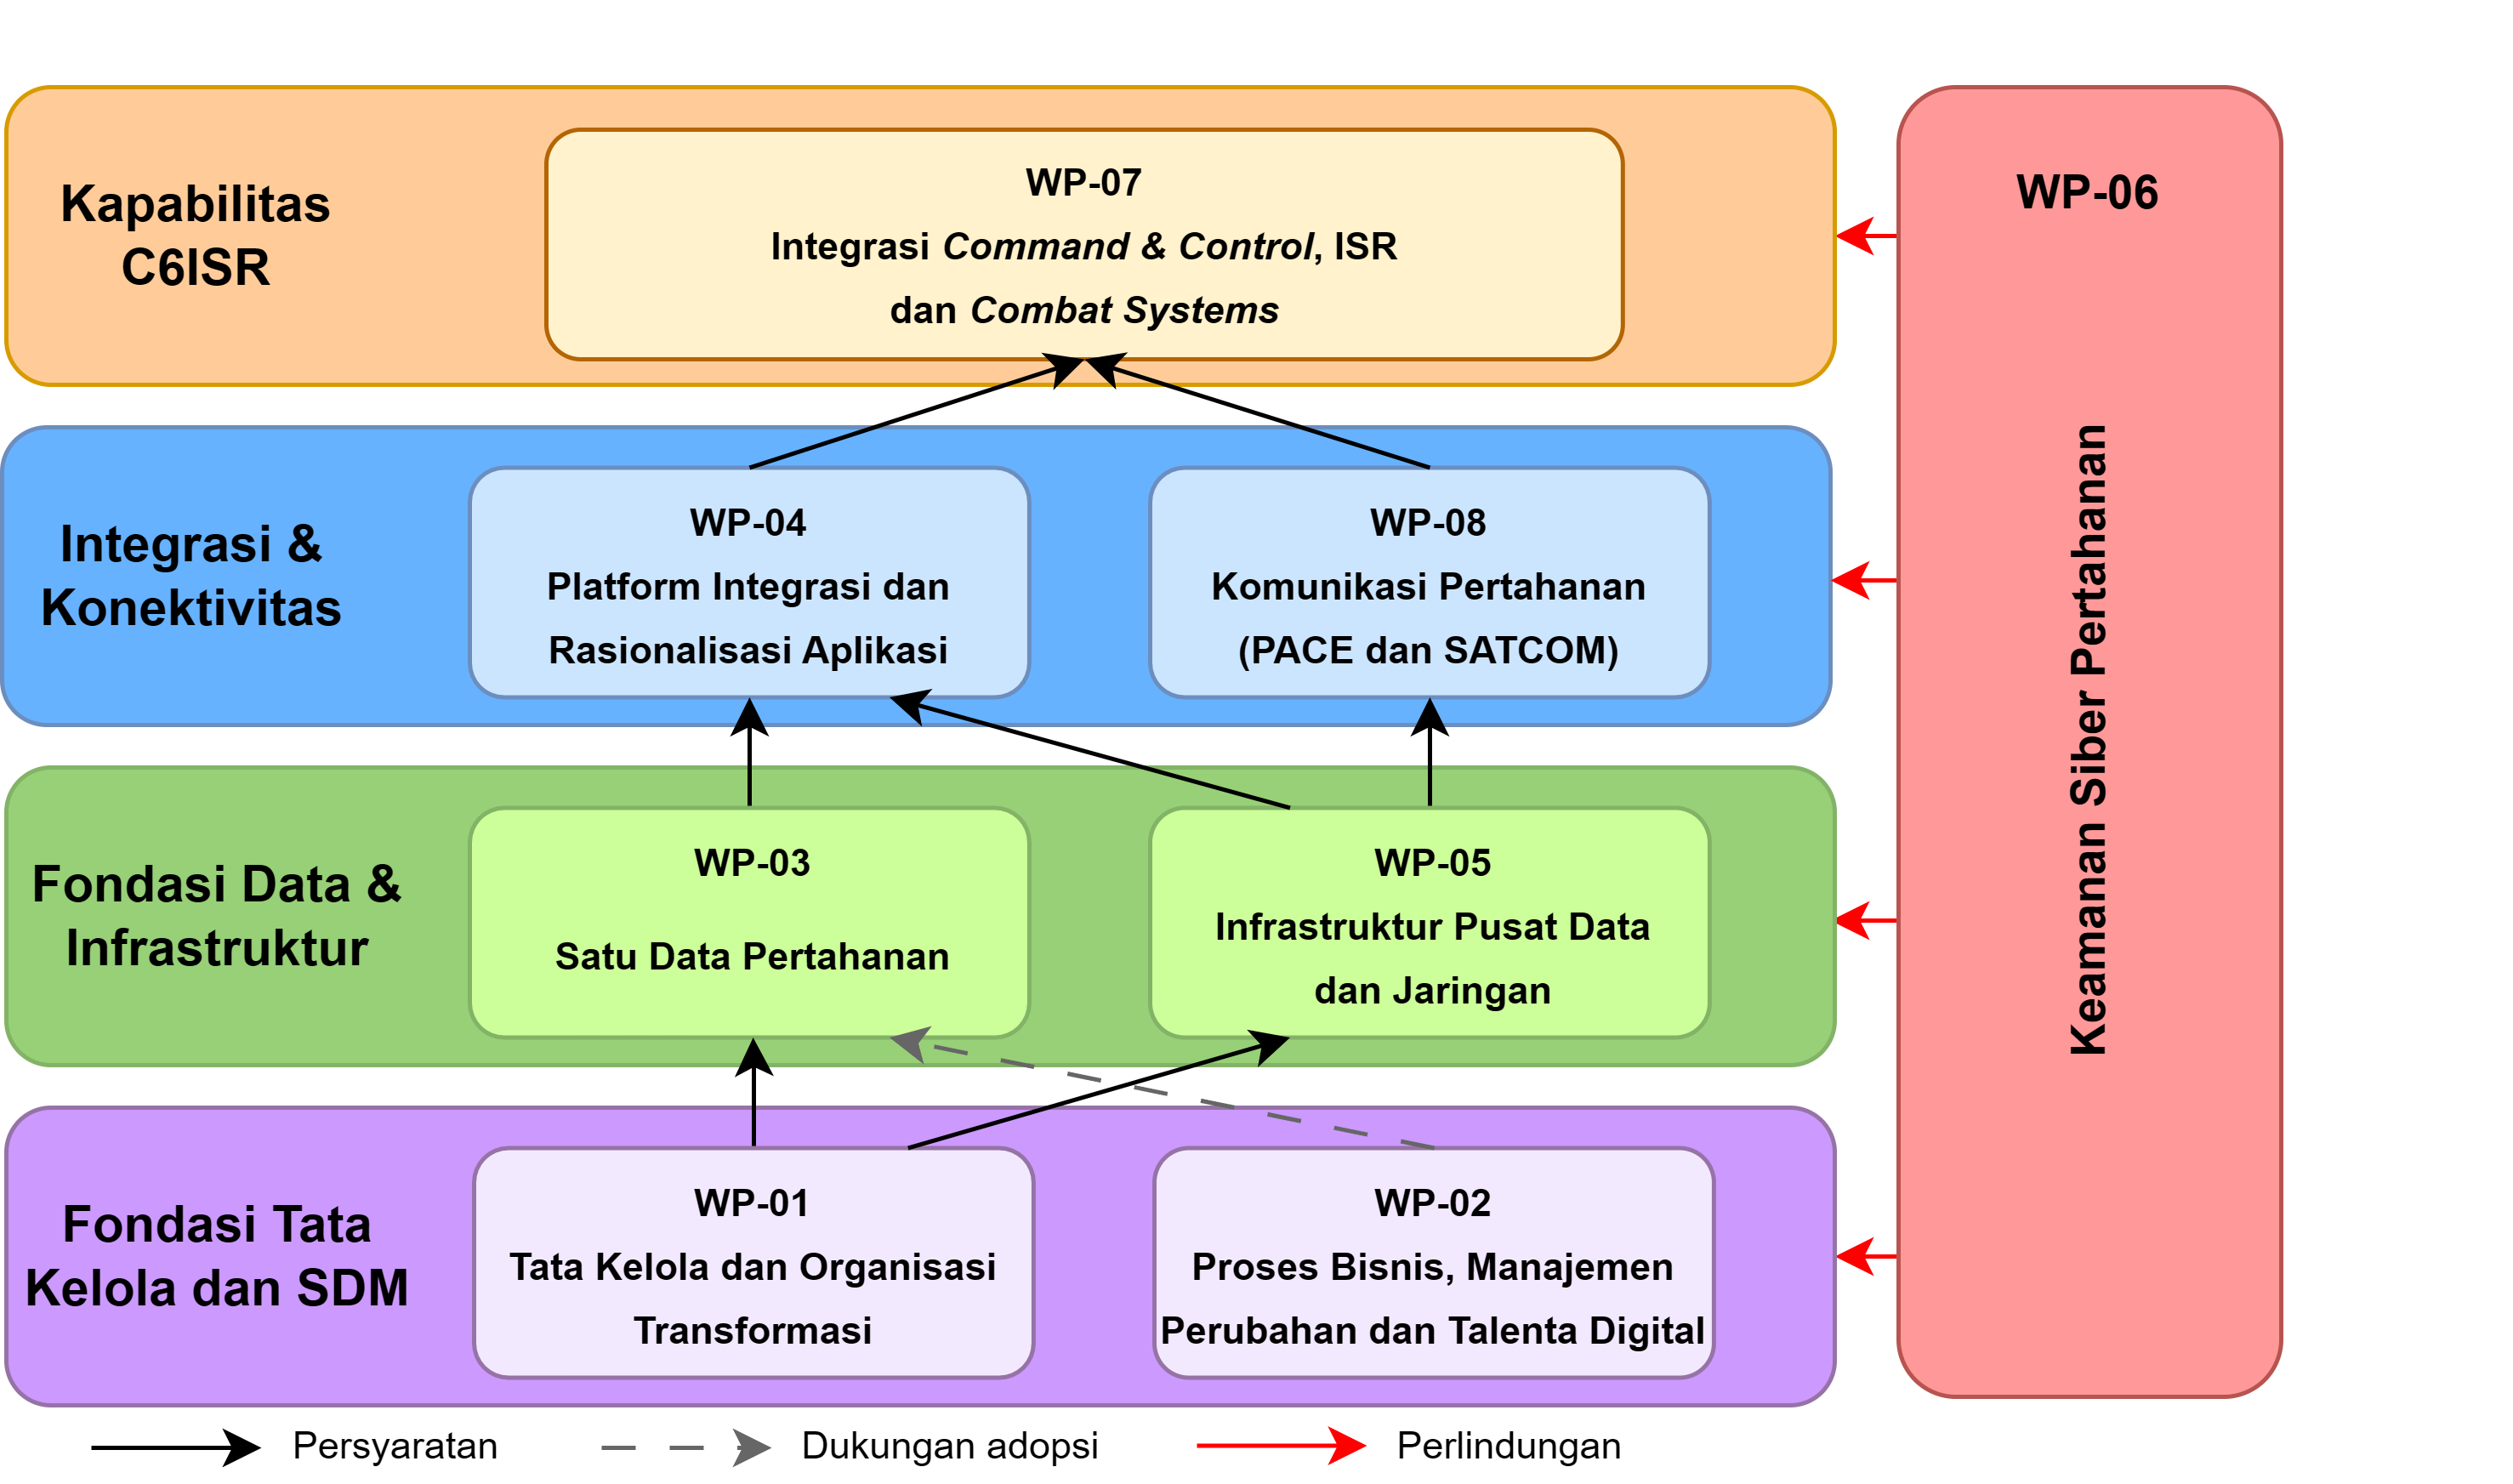
\includegraphics[width=0.90\linewidth,height=0.8\textheight,keepaspectratio]{images/Ketergantungan Work Packages.drawio.png}
\caption{Ketergantungan \textit{Work Packages}}
\label{fig:IV.27}
\end{figure}

Gambar~\ref{fig:IV.27} menyusun paket pekerjaan dalam empat lapis. WP-01 dan WP-02 menjadi fondasi karena tanpa mandat dan tata kelola transformasi, inisiatif teknis berisiko berjalan parsial. WP-03 dan WP-05 menyediakan data terstandar serta infrastruktur yang menjadi prasyarat bagi WP-04, sedangkan WP-05 juga menjadi prasyarat bagi WP-08. WP-07 baru dapat diwujudkan setelah data dapat dipertukarkan melalui WP-04 dan jalur komunikasi tersedia melalui WP-08. WP-06 digambarkan vertikal karena melindungi seluruh paket pekerjaan sejak jangka pendek.

\subsection{Kesiapan dan Risiko}
\label{sec:IV.7.4}

Tingkat kesiapan pada Tabel~\ref{tab:IV.7} dan risiko pada Tabel~\ref{tab:IV.8} dipetakan ke setiap paket pekerjaan, sebagaimana disajikan pada Tabel~\ref{tab:IV.35}.

\begingroup\small\setstretch{1.0}
\begin{longtable}{@{}>{\raggedright\arraybackslash\hspace{0pt}}p{0.091\linewidth}>{\raggedright\arraybackslash\hspace{0pt}}p{0.246\linewidth}>{\raggedright\arraybackslash\hspace{0pt}}p{0.240\linewidth}>{\raggedright\arraybackslash\hspace{0pt}}p{0.330\linewidth}@{}}
\caption{Kesiapan dan Risiko per Paket Pekerjaan}\label{tab:IV.35}\\
\toprule
\textbf{Paket} & \textbf{Kesiapan (Tingkat)} & \textbf{Risiko Utama} & \textbf{Mitigasi dalam Rencana}\\
\midrule
\endfirsthead
\multicolumn{4}{@{}l}{\small\itshape \tablename\ \thetable{} (lanjutan)}\\
\toprule
\textbf{Paket} & \textbf{Kesiapan (Tingkat)} & \textbf{Risiko Utama} & \textbf{Mitigasi dalam Rencana}\\
\midrule
\endhead
\bottomrule
\endlastfoot
\centering\arraybackslash WP-01 & Kepemimpinan dan tata kelola (Sedang); regulasi (Tinggi) & Resistensi perubahan organisasi & Mandat DTO ditetapkan sejak jangka pendek dengan dukungan pimpinan\\
\centering\arraybackslash WP-02 & SDM digital (Rendah–Sedang) & Keterbatasan SDM digital & Pelatihan, rekrutmen, dan kerja sama kelembagaan berjalan paralel dengan paket teknis\\
\centering\arraybackslash WP-03 & Data dan interoperabilitas (Rendah); regulasi (Tinggi) & Kompleksitas integrasi sistem \textit{legacy} & Standar data ditetapkan sebelum Portal Satu Data Pertahanan dibangun\\
\centering\arraybackslash WP-04 & Data dan interoperabilitas (Rendah) & Kompleksitas integrasi sistem \textit{legacy} & Integrasi bertahap melalui \textit{middleware}/API dan standar terbuka\\
\centering\arraybackslash WP-05 & Infrastruktur teknologi (Sedang) & Keterbatasan anggaran dan waktu & Investasi infrastruktur ditahapkan berdasarkan prioritas nilai\\
\centering\arraybackslash WP-06 & Keamanan siber (Sedang) & Ancaman siber selama transisi & Keamanan dasar didahulukan dan \textit{security by design} diterapkan pada setiap paket\\
\centering\arraybackslash WP-07 & Data dan interoperabilitas (Rendah) & Ketergantungan pada teknologi asing & Standar antarmuka terbuka dan persyaratan interoperabilitas dalam pengadaan alutsista\\
\centering\arraybackslash WP-08 & Infrastruktur teknologi (Sedang) & Ketergantungan pada teknologi asing; keterbatasan anggaran & SATCOM sewa atau \textit{dual-use} berpersandian; kepemilikan satelit melalui kajian\\
\end{longtable}
\endgroup

Tabel~\ref{tab:IV.35} menunjukkan bahwa WP-03, WP-04, dan WP-07 memiliki kesiapan terendah karena bergantung pada data dan interoperabilitas. Oleh karena itu, jangka pendek pada ketiga paket tersebut difokuskan pada penetapan standar yang berbiaya rendah tetapi menurunkan risiko integrasi. Sebaliknya, dukungan regulasi yang tinggi menjadi peluang untuk mempercepat WP-01 dan WP-03.

\subsection{Arsitektur Transisi}
\label{sec:IV.7.5}

Berdasarkan ketergantungan dan kesiapan tersebut, strategi implementasi yang dipilih adalah pendekatan bertahap dengan prinsip fondasi terlebih dahulu. Pendekatan ini menghasilkan dua arsitektur transisi sebelum arsitektur target tercapai, sebagaimana disajikan pada Tabel~\ref{tab:IV.36}.

\begingroup\small\setstretch{1.0}
\begin{longtable}{@{}>{\raggedright\arraybackslash\hspace{0pt}}p{0.130\linewidth}>{\raggedright\arraybackslash\hspace{0pt}}p{0.259\linewidth}>{\raggedright\arraybackslash\hspace{0pt}}p{0.259\linewidth}>{\raggedright\arraybackslash\hspace{0pt}}p{0.259\linewidth}@{}}
\caption{Arsitektur Transisi per Domain}\label{tab:IV.36}\\
\toprule
\textbf{Domain} & \textbf{Transisi Tahap 1}\newline \textbf{(Fondasi Tata Kelola dan Standar)} & \textbf{Transisi Tahap 2}\newline \textbf{(Integrasi Data dan Platform)} & \textbf{Arsitektur Target}\newline \textbf{(Pertahanan Cerdas Terintegrasi)}\\
\midrule
\endfirsthead
\multicolumn{4}{@{}l}{\small\itshape \tablename\ \thetable{} (lanjutan)}\\
\toprule
\textbf{Domain} & \textbf{Transisi Tahap 1}\newline \textbf{(Fondasi Tata Kelola dan Standar)} & \textbf{Transisi Tahap 2}\newline \textbf{(Integrasi Data dan Platform)} & \textbf{Arsitektur Target}\newline \textbf{(Pertahanan Cerdas Terintegrasi)}\\
\midrule
\endhead
\bottomrule
\endlastfoot
Bisnis & DTO dan \textit{Architecture Board} berjalan & Proses bisnis terstandar; koordinasi lintas matra terlembaga & Budaya transformasi berkelanjutan\\
Data & Penyelenggara Satu Data, klasifikasi, dan kamus data ditetapkan & Portal Satu Data Pertahanan beroperasi & Interoperabilitas dengan Portal Satu Data Indonesia\\
Aplikasi & Peta rasionalisasi aplikasi tersedia & Platform integrasi dan SSO/IAM beroperasi; aplikasi berfungsi serupa digabungkan & Aplikasi terintegrasi penuh; tata kelola portofolio terlembaga\\
Teknologi & DRC dan keamanan dasar tersedia & Virtualisasi, kontainer, jaringan tersegmentasi, dan SOC beroperasi & \textit{Data Center} Utama dan DRC aktif-aktif; kematangan keamanan siber level 3\\
C6ISR & Standar interoperabilitas, prosedur \textit{Command \& Control}, rencana PACE, dan SATCOM sewa ditetapkan & Jaringan terklasifikasi dan TPT lintas matra beroperasi; skema PACE diterapkan & Integrasi penuh ISR, \textit{Command \& Control}, dan \textit{Combat Systems}; satelit pertahanan nasional\\
\end{longtable}
\endgroup

Tabel~\ref{tab:IV.36} menunjukkan bahwa keluaran Tahap 1 sebagian besar berupa keputusan, regulasi, dan rancangan. Tahap 2 menghasilkan integrasi data dan platform, termasuk gambaran situasi bersama lintas matra, sedangkan arsitektur target mewujudkan pertahanan cerdas yang terintegrasi pada seluruh domain.

\subsection{\textit{Roadmap} Arsitektur}
\label{sec:IV.7.6}

Paket pekerjaan, ketergantungan, dan arsitektur transisi dirangkum menjadi \textit{roadmap} arsitektur terkonsolidasi, sebagaimana ditunjukkan pada Gambar~\ref{fig:IV.28}.
\begin{figure}[htbp]
\centering
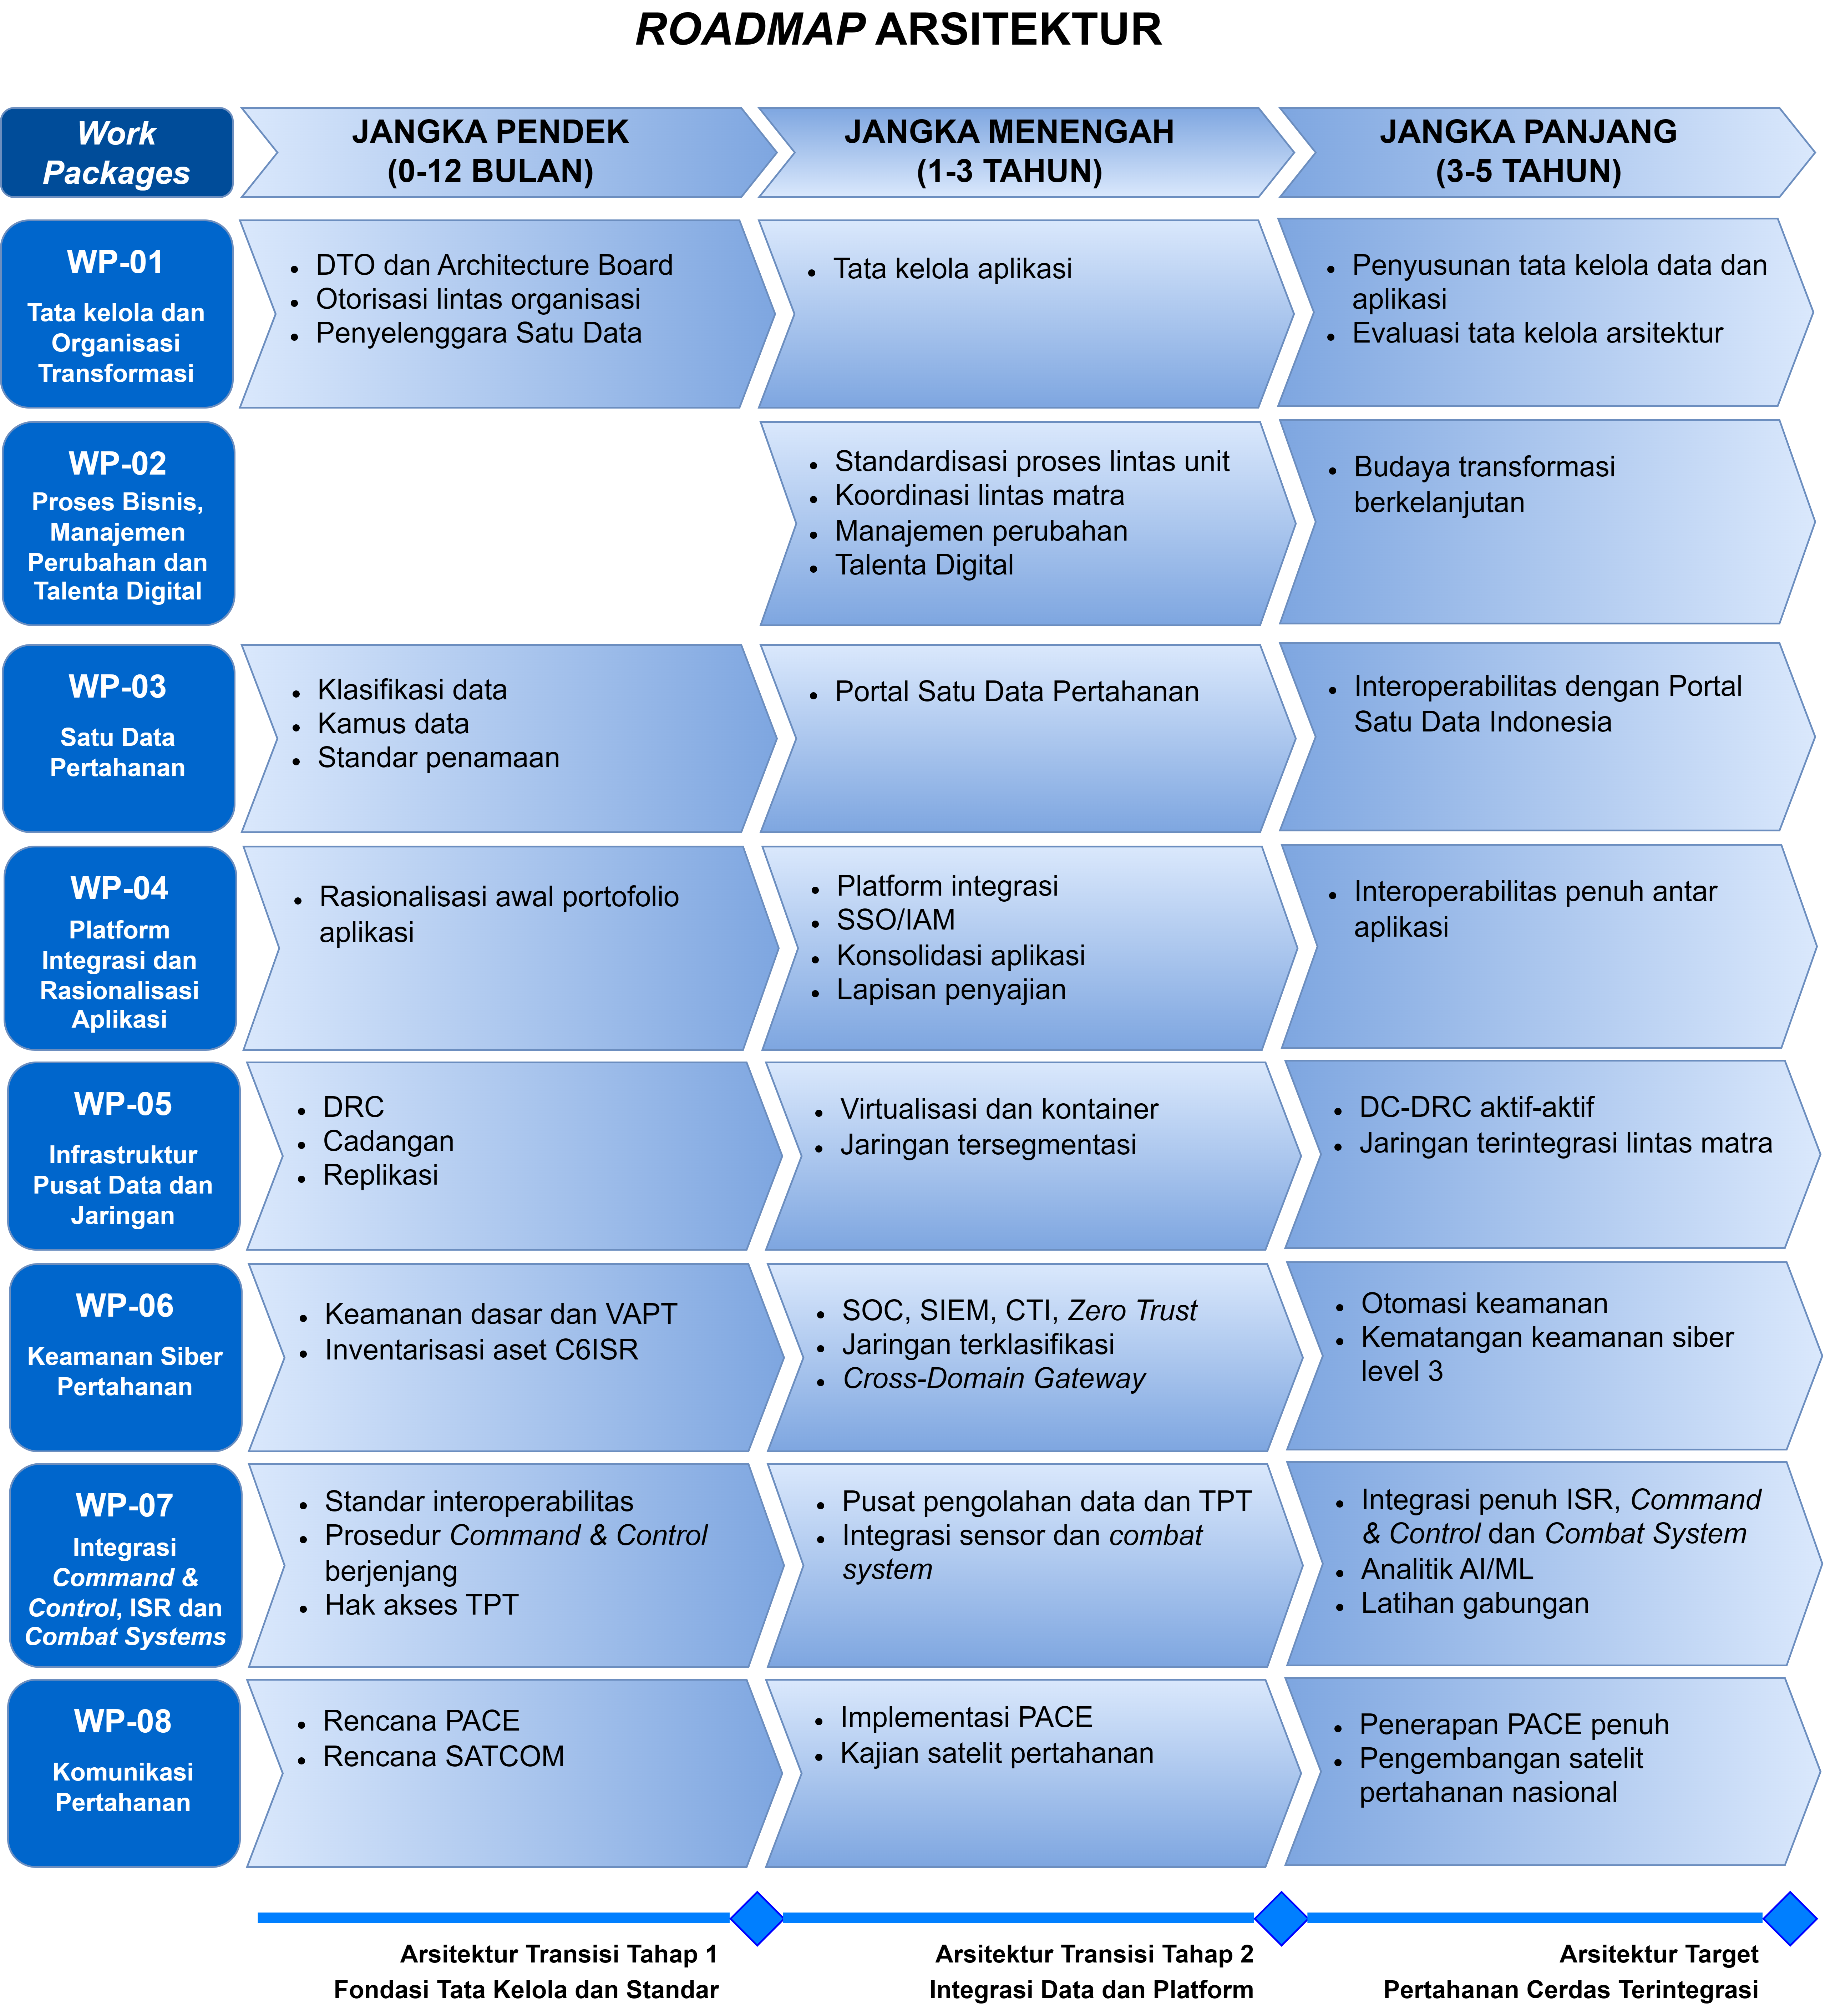
\includegraphics[width=0.89\linewidth,height=0.8\textheight,keepaspectratio]{images/Roadmap arsitektur terkonsolidasi.drawio.png}
\caption{\textit{Roadmap} Arsitektur}
\label{fig:IV.28}
\end{figure}

Gambar~\ref{fig:IV.28} menempatkan setiap paket pekerjaan pada tiga horizon waktu, sehingga \textit{roadmap} setiap fase tergabung dalam satu gambar. Penanda di bagian bawah menunjukkan saat tercapainya Arsitektur Transisi Tahap 1, Arsitektur Transisi Tahap 2, dan Arsitektur Target. WP-02 baru dimulai pada jangka menengah karena bergantung pada terbentuknya DTO, sedangkan WP-06 berjalan pada seluruh horizon sebagai pelindung paket lainnya.

\section{Fase Migration Planning}
\label{sec:IV.8}

Fase Migration Planning menyusun rencana implementasi dan migrasi berdasarkan paket pekerjaan, arsitektur transisi, dan \textit{roadmap} arsitektur. Fase ini menetapkan tata kelola implementasi, menilai manfaat dan kebutuhan sumber daya, memprioritaskan paket pekerjaan, menyusun jadwal tahun 2026–2030, serta menetapkan indikator keberhasilan.

\subsection{Tata Kelola Implementasi}
\label{sec:IV.8.1}

Rencana implementasi perlu terhubung dengan kerangka manajemen organisasi, yaitu tata kelola arsitektur, perencanaan dan penganggaran, serta pengawasan. Peran setiap pihak dalam tata kelola implementasi disajikan pada Tabel~\ref{tab:IV.37}.

\begingroup\small\setstretch{1.0}
\begin{longtable}{@{}>{\raggedright\arraybackslash\hspace{0pt}}p{0.214\linewidth}>{\raggedright\arraybackslash\hspace{0pt}}p{0.321\linewidth}>{\raggedright\arraybackslash\hspace{0pt}}p{0.402\linewidth}@{}}
\caption{Model Tata Kelola Implementasi}\label{tab:IV.37}\\
\toprule
\textbf{Peran} & \textbf{Pihak} & \textbf{Tanggung Jawab}\\
\midrule
\endfirsthead
\multicolumn{3}{@{}l}{\small\itshape \tablename\ \thetable{} (lanjutan)}\\
\toprule
\textbf{Peran} & \textbf{Pihak} & \textbf{Tanggung Jawab}\\
\midrule
\endhead
\bottomrule
\endlastfoot
Pengarah & Menteri Pertahanan; Sekretaris Jenderal & Menetapkan arah kebijakan serta menyetujui prioritas dan anggaran transformasi\\
Pengendali arsitektur & DTO dan \textit{Architecture Board} & Menetapkan standar, menilai kepatuhan proyek terhadap arsitektur, dan menetapkan kontrak arsitektur\\
Pengelola program & DTO (Bidang Strategi dan \textit{Roadmap} Transformasi Digital) & Mengoordinasikan jadwal, ketergantungan, dan pelaporan kemajuan paket pekerjaan\\
Perencana dan penganggar & Ditjen Perencanaan Pertahanan; Biro Perencanaan dan Keuangan & Menyelaraskan paket pekerjaan dengan dokumen perencanaan dan penganggaran pertahanan\\
Pelaksana & Pusat Data dan Informasi; Pusat Siber dan Intelijen Teknologi Pertahanan; satuan kerja terkait & Melaksanakan paket pekerjaan sesuai kontrak arsitektur\\
Mitra operasional & Mabes TNI dan ketiga matra & Melaksanakan dan memvalidasi paket pekerjaan C6ISR (WP-07 dan WP-08)\\
Pengawas & Inspektorat Jenderal & Mengawasi kepatuhan pelaksanaan terhadap peraturan perundang-undangan\\
\end{longtable}
\endgroup

Tabel~\ref{tab:IV.37} menunjukkan bahwa setiap proyek dalam paket pekerjaan dilaksanakan berdasarkan kontrak arsitektur (\textit{architecture contract}) antara \textit{Architecture Board} dan pelaksana. Kontrak tersebut memuat lingkup proyek, standar yang wajib dipenuhi, dan kriteria penerimaan.

\subsection{Nilai Manfaat dan Sumber Daya}
\label{sec:IV.8.2}

Nilai manfaat setiap paket pekerjaan ditentukan dari kontribusinya terhadap tujuan strategis pada Tabel~\ref{tab:IV.5}. Karena data anggaran rinci belum tersedia, kebutuhan biaya dikelompokkan ke dalam tiga kelas, yaitu rendah untuk penetapan regulasi dan penataan organisasi, sedang untuk pengembangan sistem dan perangkat lunak, serta tinggi untuk pembangunan infrastruktur fisik atau pengadaan skala besar. Hasilnya disajikan pada Tabel~\ref{tab:IV.38}.

\begingroup\small\setstretch{1.0}
\begin{longtable}{@{}>{\raggedright\arraybackslash\hspace{0pt}}p{0.097\linewidth}>{\raggedright\arraybackslash\hspace{0pt}}p{0.194\linewidth}>{\raggedright\arraybackslash\hspace{0pt}}p{0.453\linewidth}>{\raggedright\arraybackslash\hspace{0pt}}p{0.162\linewidth}@{}}
\caption{Nilai Manfaat dan Kebutuhan Sumber Daya Paket Pekerjaan}\label{tab:IV.38}\\
\toprule
\textbf{Paket} & \textbf{Tujuan Strategis (Tabel IV.5)} & \textbf{Sarana Penyampaian} & \textbf{Kelas Biaya}\\
\midrule
\endfirsthead
\multicolumn{4}{@{}l}{\small\itshape \tablename\ \thetable{} (lanjutan)}\\
\toprule
\textbf{Paket} & \textbf{Tujuan Strategis (Tabel IV.5)} & \textbf{Sarana Penyampaian} & \textbf{Kelas Biaya}\\
\midrule
\endhead
\bottomrule
\endlastfoot
\centering\arraybackslash WP-01 & \centering\arraybackslash 3, 6 & Penetapan regulasi dan penataan organisasi & \centering\arraybackslash Rendah\\
\centering\arraybackslash WP-02 & \centering\arraybackslash 1, 5 & Standardisasi proses, pelatihan, dan rekrutmen & \centering\arraybackslash Sedang\\
\centering\arraybackslash WP-03 & \centering\arraybackslash 1, 3, 6 & Penetapan regulasi data dan pengembangan sistem & \centering\arraybackslash Sedang\\
\centering\arraybackslash WP-04 & \centering\arraybackslash 1, 3, 5 & Pengembangan sistem dan penggabungan aplikasi & \centering\arraybackslash Sedang\\
\centering\arraybackslash WP-05 & \centering\arraybackslash 1, 4 & Pengadaan dan pembangunan infrastruktur & \centering\arraybackslash Tinggi\\
\centering\arraybackslash WP-06 & \centering\arraybackslash 2, 6 & Pengadaan perangkat keamanan dan pembentukan SOC & \centering\arraybackslash Sedang\\
\centering\arraybackslash WP-07 & \centering\arraybackslash 1, 3, 4 & Standardisasi, pengembangan sistem, dan integrasi alutsista bersama Mabes TNI & \centering\arraybackslash Tinggi\\
\centering\arraybackslash WP-08 & \centering\arraybackslash 1, 2, 4 & Sewa kapasitas, pengadaan perangkat komunikasi, dan pengembangan satelit & \centering\arraybackslash Tinggi\\
\end{longtable}
\endgroup

Tabel~\ref{tab:IV.38} menunjukkan bahwa WP-03, WP-04, WP-07, dan WP-08 mendukung tiga tujuan strategis sekaligus. Namun, WP-05, WP-07, dan WP-08 membutuhkan biaya tertinggi karena melibatkan infrastruktur fisik, integrasi alutsista, dan satelit.

\subsection{Prioritas Paket Pekerjaan}
\label{sec:IV.8.3}

Prioritas paket pekerjaan ditentukan berdasarkan empat kriteria dengan skor 1–3, yaitu:
\begin{enumerate}[label=\arabic*.]
\item Manfaat strategis, berdasarkan jumlah tujuan strategis yang didukung pada Tabel~\ref{tab:IV.38} (satu tujuan = 1, dua tujuan = 2, tiga tujuan = 3);
\item Biaya, berdasarkan kelas biaya pada Tabel~\ref{tab:IV.38} (tinggi = 1, sedang = 2, rendah = 3);
\item Risiko, berdasarkan tingkat kesiapan terendah pada Tabel~\ref{tab:IV.35} (rendah atau rendah–sedang = 1, sedang = 2, tinggi = 3); dan
\item Ketergantungan, berdasarkan jumlah paket yang bergantung pada paket tersebut pada Gambar~\ref{fig:IV.27} (tidak ada = 1, satu paket = 2, dua paket atau lebih = 3).
\end{enumerate}

Skor keempat kriteria dijumlahkan dengan rentang 4–12. Paket dengan skor 9–12 ditetapkan sebagai Prioritas I, skor 7–8 sebagai Prioritas II, dan skor 4–6 sebagai Prioritas III. Hasilnya disajikan pada Gambar~\ref{fig:IV.29}.
\begin{figure}[htbp]
\centering
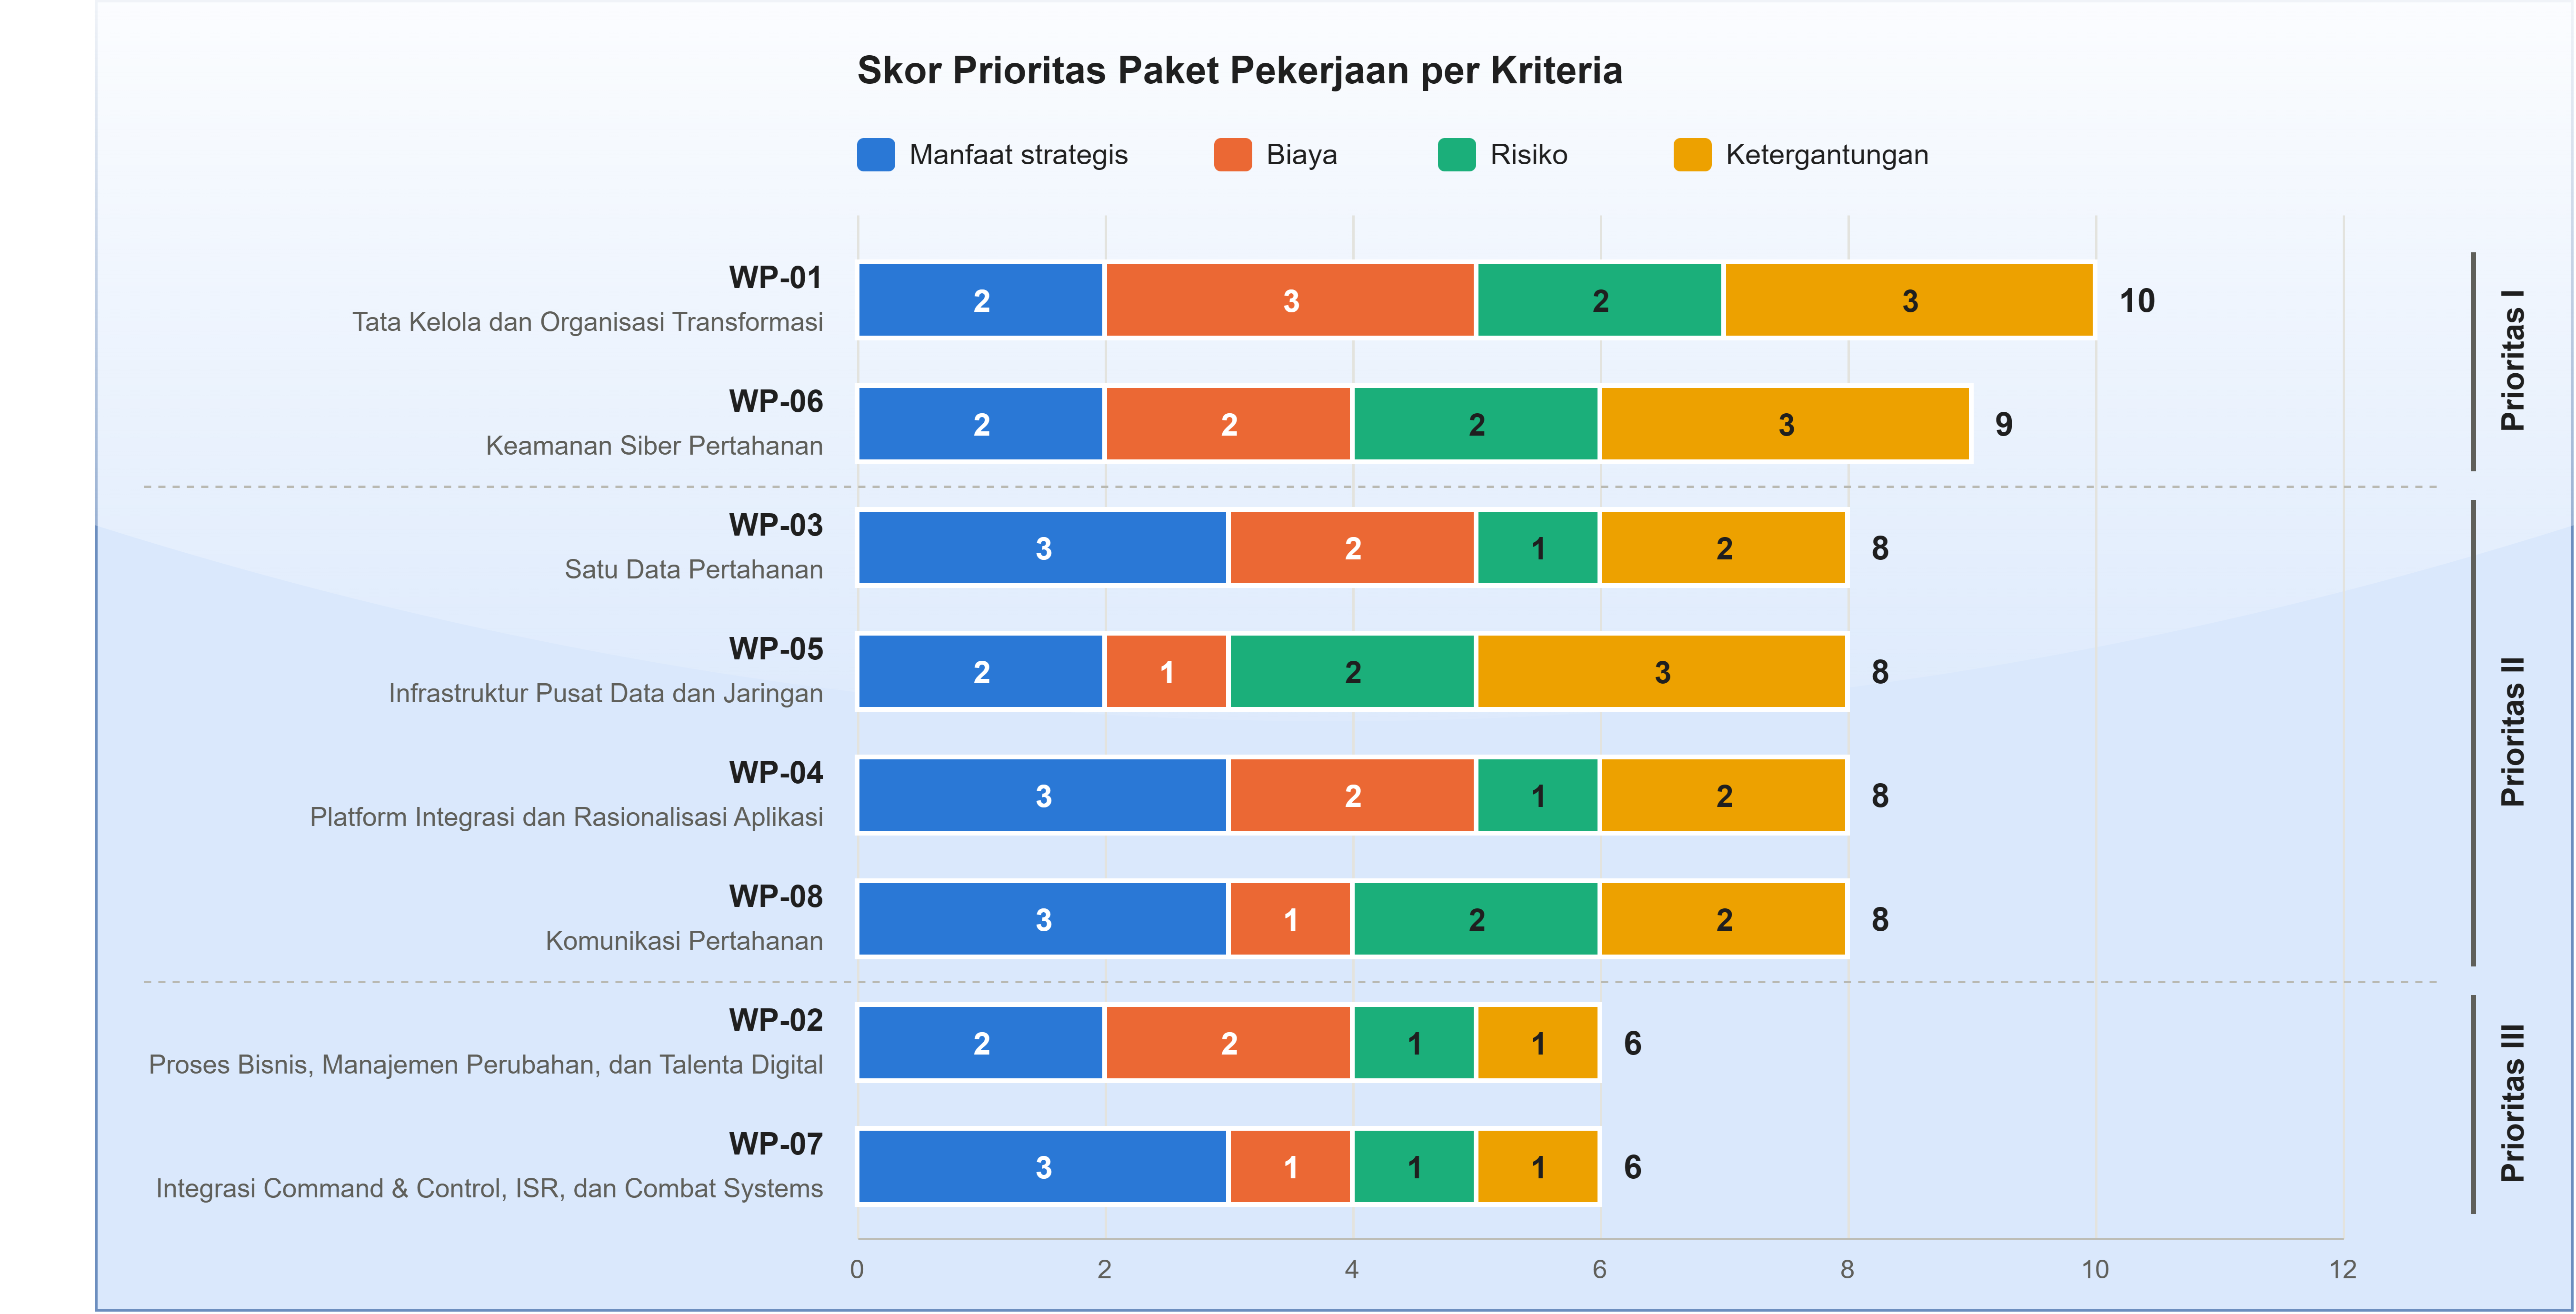
\includegraphics[width=0.99\linewidth,height=0.8\textheight,keepaspectratio]{images/Skor_Prioritas_Paket_Pekerjaan.drawio.png}
\caption{Skor Prioritas Paket Pekerjaan}
\label{fig:IV.29}
\end{figure}

Gambar~\ref{fig:IV.29} menunjukkan bahwa Prioritas I terdiri atas WP-01 dan WP-06 karena keduanya menjadi prasyarat atau pelindung bagi paket lainnya dengan biaya yang relatif terjangkau. Skor ketergantungan WP-06 dihitung dari perannya melindungi seluruh paket. Prioritas II terdiri atas WP-03, WP-05, WP-04, dan WP-08, dengan WP-03 dan WP-05 didahulukan sesuai ketergantungan pada Gambar~\ref{fig:IV.27}. Prioritas III terdiri atas WP-02 dan WP-07.

Prioritas menunjukkan urutan pemusatan sumber daya, bukan tingkat kepentingan. WP-07 memiliki manfaat strategis tertinggi sebagai inti C6ISR, tetapi berada pada Prioritas III karena biayanya tinggi, kesiapannya rendah, dan bergantung pada hampir seluruh paket lainnya.

\subsection{Rencana Implementasi dan Migrasi 2026–2030}
\label{sec:IV.8.4}

Berdasarkan prioritas tersebut, paket pekerjaan dijadwalkan pada tahun 2026–2030. Jangka pendek ditempatkan pada tahun 2026, jangka menengah pada 2027–2028, dan jangka panjang pada 2029–2030, sehingga target kematangan keamanan siber level 3 pada tahun 2029 berada dalam jangka panjang. Jadwal per semester disajikan pada Gambar~\ref{fig:IV.30}.
\begin{figure}[htbp]
\centering
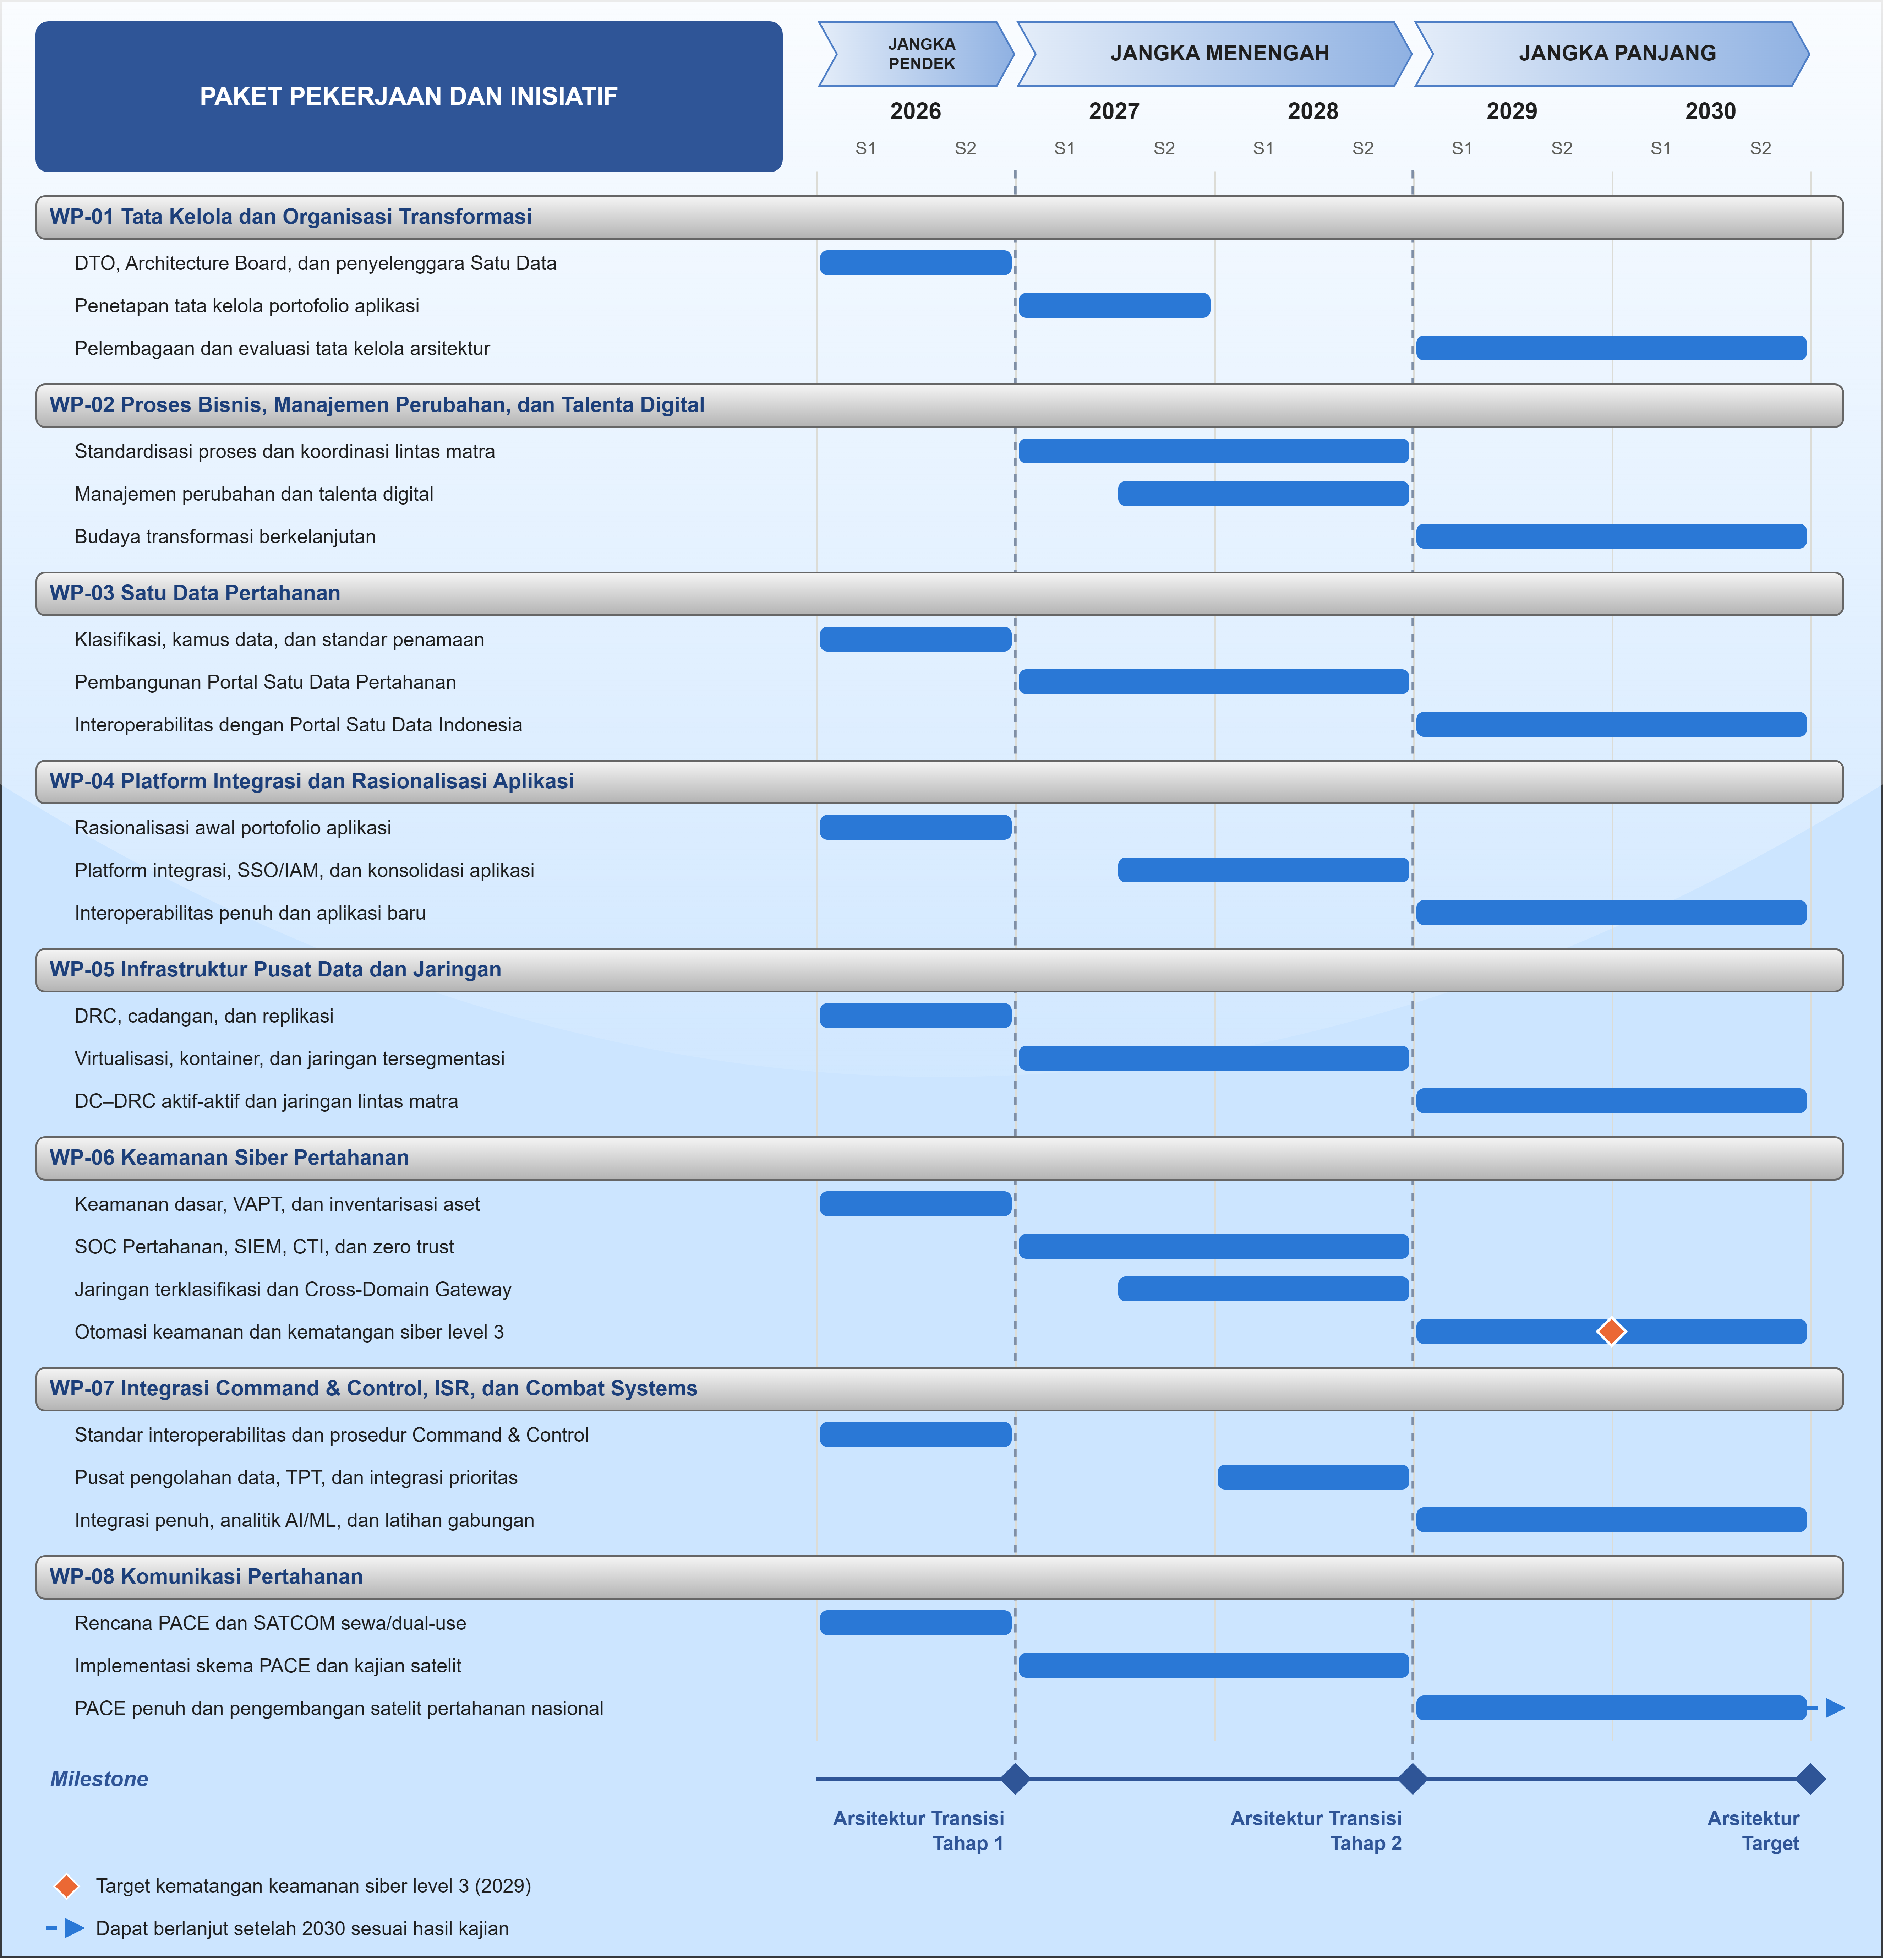
\includegraphics[width=0.89\linewidth,height=0.8\textheight,keepaspectratio]{images/Jadwal_Implementasi_dan_Migrasi.drawio.png}
\caption{Jadwal Implementasi dan Migrasi 2026–2030}
\label{fig:IV.30}
\end{figure}

Gambar~\ref{fig:IV.30} menunjukkan bahwa inisiatif dalam satu horizon tidak selalu dimulai bersamaan. Platform integrasi (WP-04) dimulai pada semester kedua 2027 setelah pembangunan Portal Satu Data Pertahanan dan virtualisasi berjalan, sedangkan pusat pengolahan data dan TPT (WP-07) dimulai pada 2028 setelah jaringan terklasifikasi (WP-06) mulai dibangun. Pengembangan satelit pertahanan dapat berlanjut setelah 2030 karena bergantung pada hasil kajian dan ketersediaan slot orbit.

Jadwal tersebut dilaksanakan dalam tiga tahap migrasi. Setiap tahap diakhiri dengan tinjauan \textit{Architecture Board} sebelum tahap berikutnya dimulai, sebagaimana disajikan pada Tabel~\ref{tab:IV.39}.

\begingroup\small\setstretch{1.0}
\begin{longtable}{@{}>{\raggedright\arraybackslash\hspace{0pt}}p{0.259\linewidth}>{\raggedright\arraybackslash\hspace{0pt}}p{0.130\linewidth}>{\raggedright\arraybackslash\hspace{0pt}}p{0.291\linewidth}>{\raggedright\arraybackslash\hspace{0pt}}p{0.227\linewidth}@{}}
\caption{Tahapan Migrasi}\label{tab:IV.39}\\
\toprule
\textbf{Tahap} & \textbf{Periode} & \textbf{Fokus Paket Pekerjaan} & \textbf{Titik Keputusan}\\
\midrule
\endfirsthead
\multicolumn{4}{@{}l}{\small\itshape \tablename\ \thetable{} (lanjutan)}\\
\toprule
\textbf{Tahap} & \textbf{Periode} & \textbf{Fokus Paket Pekerjaan} & \textbf{Titik Keputusan}\\
\midrule
\endhead
\bottomrule
\endlastfoot
Tahap 1: Fondasi Tata Kelola dan Standar & \centering\arraybackslash 2026 & WP-01 dan WP-06 (Prioritas I); inisiatif jangka pendek pada paket lainnya & Tinjauan Arsitektur Transisi Tahap 1\\
Tahap 2: Integrasi Data dan Platform & \centering\arraybackslash 2027–2028 & WP-03, WP-05, WP-04, dan WP-08 (Prioritas II); WP-02 dimulai & Tinjauan Arsitektur Transisi Tahap 2\\
Tahap 3: Pertahanan Cerdas Terintegrasi & \centering\arraybackslash 2029–2030 & WP-07 dan WP-02 (Prioritas III); penyelesaian seluruh paket & Evaluasi arsitektur target dan \textit{Request for Architecture Work} siklus berikutnya\\
\end{longtable}
\endgroup

Tabel~\ref{tab:IV.39} menunjukkan bahwa setiap tahap memiliki titik keputusan. Apabila suatu tahap belum tercapai, \textit{Architecture Board} dapat menyesuaikan jadwal tahap berikutnya tanpa mengubah arsitektur target.

\subsection{Indikator Keberhasilan}
\label{sec:IV.8.5}

Indikator keberhasilan disusun pada dua tingkat. Tingkat pertama adalah indikator capaian tahap, yaitu kondisi arsitektur transisi pada Tabel~\ref{tab:IV.36} yang digunakan \textit{Architecture Board} pada setiap titik keputusan. Tingkat kedua adalah indikator dampak yang mengaitkan setiap tantangan pada Tabel~\ref{tab:II.1} dengan nilai awal, target, dan paket pekerjaan yang menanganinya, sebagaimana disajikan pada Tabel~\ref{tab:IV.40}.

\begingroup\small\setstretch{1.0}
\begin{longtable}{@{}>{\raggedright\arraybackslash\hspace{0pt}}p{0.060\linewidth}>{\raggedright\arraybackslash\hspace{0pt}}p{0.133\linewidth}>{\raggedright\arraybackslash\hspace{0pt}}p{0.230\linewidth}>{\raggedright\arraybackslash\hspace{0pt}}p{0.166\linewidth}>{\raggedright\arraybackslash\hspace{0pt}}p{0.166\linewidth}>{\raggedright\arraybackslash\hspace{0pt}}p{0.091\linewidth}@{}}
\caption{Indikator Dampak Transformasi Digital Kemhan RI}\label{tab:IV.40}\\
\toprule
\textbf{No.} & \textbf{Dimensi} & \textbf{Indikator} & \textbf{Nilai Awal} & \textbf{Target} & \textbf{Paket}\\
\midrule
\endfirsthead
\multicolumn{6}{@{}l}{\small\itshape \tablename\ \thetable{} (lanjutan)}\\
\toprule
\textbf{No.} & \textbf{Dimensi} & \textbf{Indikator} & \textbf{Nilai Awal} & \textbf{Target} & \textbf{Paket}\\
\midrule
\endhead
\bottomrule
\endlastfoot
\centering\arraybackslash 1 & Tata kelola & Keberadaan DTO dan \textit{Architecture Board} & Belum ada & Ditetapkan (Tahap 1) & \centering\arraybackslash WP-01\\
\centering\arraybackslash 2 & Data & Persentase set data pada Portal Satu Data Pertahanan yang memiliki kamus data dan klasifikasi & Belum ada & 100\% & \centering\arraybackslash WP-03\\
\centering\arraybackslash 3 & Aplikasi & Jumlah aplikasi khusus & 71 aplikasi & 42 aplikasi terintegrasi & \centering\arraybackslash WP-04\\
\centering\arraybackslash 4 & Teknologi & Konfigurasi pusat data & Satu \textit{Data Center} tanpa DRC & \textit{Data Center} Utama dan DRC aktif-aktif & \centering\arraybackslash WP-05\\
\centering\arraybackslash 5 & Keamanan siber & Tingkat kematangan keamanan siber & Level 1–2 & Level 3 (2029) & \centering\arraybackslash WP-06\\
\centering\arraybackslash 6 & SDM & Ketersediaan katalog kompetensi dan analisis kesenjangan keterampilan digital & Belum ada & Tersedia dan diperbarui berkala & \centering\arraybackslash WP-02\\
\centering\arraybackslash 7 & Operasional & Ketersediaan TPT lintas matra & Belum ada & Beroperasi (Tahap 2) & \centering\arraybackslash WP-07\\
\centering\arraybackslash 8 & SPBE & Indeks SPBE Kemhan RI & 3,43, predikat Baik (2023) \cite{Pusdatin2024} & $\geq$ 3,5, predikat Sangat Baik & \centering\arraybackslash WP-01\newline s.d.\newline WP-06\\
\end{longtable}
\endgroup

Tabel~\ref{tab:IV.40} menunjukkan bahwa setiap tantangan pada Tabel~\ref{tab:II.1} memiliki indikator yang terukur. Indikator dampak diukur oleh Kemhan RI setelah implementasi, sehingga berada di luar cakupan evaluasi penelitian ini yang bersifat \textit{ex-ante}.

Dengan tersusunnya rencana implementasi dan migrasi, perancangan arsitektur pada penelitian ini selesai. Fase Implementation Governance dan Architecture Change Management dilaksanakan ketika implementasi berjalan, sehingga berada di luar cakupan penelitian ini.
